
% Compile with XeLaTeX.
\documentclass[14pt,a4paper]{extreport}
\usepackage{fontspec}
\usepackage{polyglossia}
\setmainlanguage{russian}
\setotherlanguage{english}
\setmainfont{Times New Roman}
\setmonofont{Courier New}
\newfontfamily\cyrillicfonttt{Courier New}
\usepackage[left=2cm,right=1cm,top=2cm,bottom=2cm]{geometry}
\usepackage{setspace}
\onehalfspacing
\usepackage{indentfirst}
\setlength{\parindent}{1.25cm}
\usepackage{graphicx}
\usepackage{float}
\usepackage{booktabs}
\usepackage{longtable}
\usepackage{array}
\setlength{\tabcolsep}{3pt}
\usepackage{amsmath,amssymb}
\usepackage{pdfpages}
\usepackage{eso-pic}
\usepackage{hyperref}
\usepackage{xurl}
\usepackage{caption}
\usepackage{enumitem}
\usepackage{titlesec}
\hypersetup{colorlinks=true,linkcolor=black,citecolor=black,urlcolor=blue}
\renewcommand{\bibname}{Список используемых источников}
\titleformat{\chapter}{\normalfont\bfseries\fontsize{18}{22}\selectfont}{\thechapter.}{1em}{}
\titleformat{\section}{\normalfont\bfseries\fontsize{16}{20}\selectfont}{\thesection}{1em}{}
\titleformat{\subsection}{\normalfont\bfseries\fontsize{14}{18}\selectfont}{\thesubsection}{1em}{}
\captionsetup{font=small,labelfont=bf}
\newcommand{\todo}[1]{\textbf{[Уточнить: #1]}}
\begin{document}

\begin{titlepage}
\begin{center}
ФЕДЕРАЛЬНОЕ ГОСУДАРСТВЕННОЕ АВТОНОМНОЕ ОБРАЗОВАТЕЛЬНОЕ УЧРЕЖДЕНИЕ\\
ВЫСШЕГО ОБРАЗОВАНИЯ\\
\textbf{«НАЦИОНАЛЬНЫЙ ИССЛЕДОВАТЕЛЬСКИЙ УНИВЕРСИТЕТ\\ «ВЫСШАЯ ШКОЛА ЭКОНОМИКИ»}\\[0.5cm]
Московский институт электроники и математики\\[2.2cm]

Раджабов Рустам Русланович\\[1.0cm]

\textbf{Разработка и сравнение моделей классификации удовлетворённости клиентов\\
на основе методов машинного обучения}\\[1.0cm]

Выпускная квалификационная работа студента образовательной программы бакалавриата\\
«Прикладная математика»\\
по направлению подготовки 01.03.04 «Прикладная математика»\\[2.0cm]
\end{center}

\begin{flushright}
Студент: Раджабов Рустам Русланович\\[0.8cm]
\rule{4cm}{0.4pt}\\[0.5cm]
Руководитель ВКР: Зонтов Юрий Владимирович
\end{flushright}

\vfill
\begin{center}
Москва 2026 г.
\end{center}
\end{titlepage}


\includepdf[
    pages=1,
    pagecommand={\thispagestyle{empty}\AddToShipoutPictureFG*{\put(383,130){\includegraphics[width=86.2pt]{файлы_по_отчету/signature_overlay.png}}}}
]{файлы_по_отчету/ТЗ.pdf}

\includepdf[
    pages=2,
    pagecommand={\thispagestyle{empty}\AddToShipoutPictureFG*{\put(383,746){\includegraphics[width=86.2pt]{файлы_по_отчету/signature_overlay.png}}}}
]{файлы_по_отчету/ТЗ.pdf}

\chapter*{Аннотация}
В выпускной квалификационной работе исследуется задача прогнозирования удовлетворенности пассажиров авиаперевозок на основе данных пассажирских опросов. Целью работы является построение и сравнительная оценка моделей машинного обучения, способных классифицировать пассажиров на удовлетворенных и неудовлетворенных, а также выявлять факторы, связанные с итоговой оценкой клиента. В работе рассмотрены Logistic Regression, KNN, Decision Tree, Random Forest, XGBoost и нейронная сеть. Для всех моделей использован единый pipeline обработки данных, включающий обработку пропусков, кодирование категориальных признаков и масштабирование числовых признаков. Качество моделей оценивалось не только по F1-macro, accuracy, precision и recall, но и через ROC-AUC, анализ порога классификации, матрицу ошибок, доверительные интервалы, кривые обучения, анализ устойчивости, анализ групповой справедливости и перестановочную важность признаков. Наилучшее качество среди рассмотренных моделей показал XGBoost, что согласуется с практикой применения градиентного бустинга на табличных данных. Практическая значимость работы состоит в возможности использовать полученные результаты как основу для системы поддержки принятия решений по улучшению пассажирского опыта.

\chapter*{Abstract}
This bachelor thesis studies the problem of airline passenger satisfaction prediction using passenger survey data. The goal of the study is to build and compare machine learning models that classify passengers as satisfied or dissatisfied and identify service factors associated with the final customer assessment. The study evaluates Logistic Regression, KNN, Decision Tree, Random Forest, XGBoost, and a neural network. A unified preprocessing pipeline is used for all models, including missing value handling, categorical feature encoding, and numerical feature scaling. Model performance is assessed not only by F1-macro, accuracy, precision, and recall, but also by ROC-AUC, threshold analysis, confusion matrices, confidence intervals, learning curves, robustness analysis, group fairness analysis, and permutation feature importance. XGBoost achieved the best overall performance, which is consistent with the strong empirical performance of gradient boosting methods on tabular data. The practical value of the study is that its results can support decision-making systems aimed at improving airline passenger experience.

\tableofcontents
\clearpage


\chapter{Введение}
\section{Предметная область}
Предметной областью работы является анализ пассажирского опыта в авиационной отрасли. Авиаперевозка включает не только сам перелет, но и последовательность процессов до и после него: покупку билета, прибытие в аэропорт, регистрацию, прохождение контроля безопасности, ожидание посадки, пользование сервисами терминала, получение багажа и выход из аэропорта. Каждый из этих этапов может влиять на итоговую удовлетворенность пассажира.

Объектом исследования являются данные пассажирских опросов, содержащие оценки отдельных элементов сервиса, сведения о типе перелета, характеристиках пассажира и процессе прохождения аэропортовых процедур. Предметом исследования являются методы машинного обучения и способы их оценки при решении задачи бинарной классификации удовлетворенности пассажиров. В данной работе пассажиры разделяются на два класса: удовлетворенные и неудовлетворенные. Такое разделение позволяет перейти от описательного анализа анкет к прикладной задаче прогнозирования клиентского опыта.

\section{Актуальность проблемы}
В последние годы транспортная отрасль активно переходит к использованию методов анализа данных и систем искусственного интеллекта для повышения качества обслуживания клиентов. Авиакомпании, аэропорты и регуляторы рассматривают данные как один из ключевых ресурсов для повышения операционной эффективности, персонализации сервиса и улучшения пассажирского опыта.

Данный тезис подтверждается отраслевыми документами и материалами международных организаций. Международная организация гражданской авиации ICAO рассматривает искусственный интеллект и big data analytics как значимые инструменты для развития безопасной, эффективной и устойчивой авиации. IATA указывает, что данные становятся основой трансформации авиационной отрасли, включая повышение операционной эффективности, устойчивости и качества клиентского опыта. ACI World связывает цифровую трансформацию аэропортов с использованием real-time data, smart analytics, пассажирских опросов, benchmarking, passenger segmentation и journey mapping для улучшения качества обслуживания пассажиров.

При этом применение современных систем машинного обучения в авиационной отрасли продолжает развиваться не только с точки зрения качества предсказаний, но и с точки зрения надежности, интерпретируемости, устойчивости и безопасности таких систем. Например, EASA в документе \textit{Artificial Intelligence Roadmap 2.0} рассматривает вопросы доверия к AI-системам, explainability, safety, data governance и регулирования искусственного интеллекта в авиации. В документе \textit{Artificial Intelligence Concept Paper Issue 2} отдельно выделяются learning assurance, AI explainability и ethics-based assessment как важные элементы безопасного и надежного применения ML-систем в авиационной среде.

Дополнительную актуальность работе придает тот факт, что современные ML-системы должны оцениваться не только по итоговой метрике качества классификации, но и по ряду дополнительных характеристик: устойчивости к шуму и искажению данных, вычислительной эффективности, интерпретируемости результатов, справедливости модели по отношению к различным группам пользователей, а также стабильности качества при изменении порога классификации. Необходимость такой расширенной оценки подтверждается современными подходами к управлению рисками искусственного интеллекта. Например, NIST AI Risk Management Framework рассматривает оценку AI-систем через характеристики trustworthy AI, а не только через точность предсказаний. Среди таких характеристик NIST выделяет validity and reliability, robustness, transparency, explainability and interpretability, fairness и bias management.

Отдельной проблемой исследований в данной предметной области является проверяемость используемых данных. Во многих альтернативных учебных и прикладных работах по прогнозированию удовлетворенности пассажиров используется датасет \textit{Airline Passenger Satisfaction}, опубликованный на Kaggle пользователем Teejmahal20 \cite{kaggle-old}. В описании этого набора указано, что он был очищен и модифицирован на основе другого Kaggle-датасета пользователя John D, который является одним из исходных источников распространения данного набора \cite{john-customer-satisfaction}. Однако на страницах этих датасетов не приведены первичные документы, владелец данных, методика сбора опросов или ссылка на организацию, проводившую исследование. Поэтому проверить, что данные действительно получены из реального пассажирского опроса, невозможно.

В ходе исследования было установлено, что указанный набор данных широко переиспользуется в учебных материалах и проектах по анализу данных, включая программу Google Data Analytics и учебные проекты IIT Roorkee \cite{coursera-google-da,iit-roorkee-project}. При этом такие повторные использования не раскрывают первичный источник данных и не решают проблему верификации. В обсуждении исходного Kaggle-набора другие участники также поднимали вопрос о происхождении данных, однако автор не предоставил подтверждающих материалов \cite{kaggle-source-discussion}. Проверка сайтов соответствующих организаций и поиск связанных материалов также не позволили найти сведения о процедуре сбора, структуре анкеты и владельце исходных данных. Следовательно, популярность этого датасета не является свидетельством его подлинности.

В данной работе поэтому используется другой источник: данные пассажирских опросов Министерства транспорта Бразилии \cite{brazil-data}. В отличие от распространенного Kaggle-набора, этот источник является верифицируемым, поскольку данные опубликованы на государственном портале открытых данных, представлены в виде первичных файлов и сопровождаются материалами, позволяющими объяснить происхождение признаков и методологические особенности опроса.

Таким образом, задача сравнительного исследования моделей машинного обучения для прогнозирования удовлетворенности пассажиров представляет как практический, так и исследовательский интерес.

\section{Цель работы}
Целью работы является построение и сравнительное исследование моделей машинного обучения для прогнозирования удовлетворенности пассажиров авиаперевозок на основе данных пассажирских опросов. Модели должны по набору признаков пассажира и оценок отдельных элементов сервиса определять, относится ли пассажир к классу удовлетворенных или неудовлетворенных.

Дополнительной целью является не только выбор модели с наилучшим качеством классификации, но и анализ ее применимости в практическом сценарии. Поэтому модели сравниваются не только по стандартным метрикам качества, но и по устойчивости, интерпретируемости, поведению на разных группах пассажиров, чувствительности к порогу классификации и вычислительной эффективности.

\section{Постановка задачи}
Для достижения цели работы необходимо решить следующие задачи:
\begin{enumerate}
    \item исследовать исходные источники данных об удовлетворенности пассажиров и выбрать проверяемый набор данных;
    \item сформировать сбалансированный датасет для бинарной классификации удовлетворенности пассажиров;
    \item реализовать единый pipeline предобработки данных, включающий обработку пропусков, кодирование категориальных признаков и масштабирование числовых признаков;
    \item обучить и настроить несколько моделей машинного обучения: Logistic Regression, KNN, Decision Tree, Random Forest, XGBoost и Neural Network;
    \item сравнить модели по F1 метрикам, accuracy, balanced accuracy, precision, recall и ROC-AUC;
    \item провести расширенный анализ моделей: кривые обучения, анализ справедливости модели, анализ ошибок модели, анализ порога классификации, анализ производительности, анализ устойчивости, перестановочная важность признаков;
    \item определить наиболее подходящую модель и показать возможные сценарии практического применения моделей.
\end{enumerate}

\section{Научная новизна и практическая значимость}
Научная новизна работы заключается в двух аспектах. Во-первых, работа проводится на верифицируемом датасете, в отличие от альтернативных работ, которые выполняются на неверифицируемом датасете. Во-вторых, в работе проводится комплексное сравнительное исследование нескольких классов моделей применительно к задаче прогнозирования удовлетворенности пассажиров. В отличие от простого сравнения моделей только по accuracy или F1-score, в работе используется расширенная схема оценки качества, включающая кросс-валидацию, анализ доверительных интервалов метрик, ROC-AUC, анализ порога классификации, матрицу ошибок, анализ ошибок, кривые обучения, перестановочную важность признаков, анализ устойчивости модели и анализ групповой справедливости.

Практическая значимость работы состоит в том, что результаты исследования могут использоваться как основа для построения системы поддержки принятия решений в авиакомпании или аэропорту. Такая система может помогать выявлять неудовлетворенных пассажиров, определять наиболее значимые факторы сервиса и выбирать направления улучшения обслуживания с учетом ожидаемого влияния на удовлетворенность клиентов.


\chapter{Используемые модели машинного обучения}
\section{Logistic Regression}
Логистическая регрессия является линейной моделью для оценки апостериорной вероятности класса. В соответствии с изложением в \cite{hastie}, для бинарной классификации логарифм отношения вероятностей двух классов задается линейной функцией признаков. Пусть объект описывается вектором признаков $x \in \mathbb{R}^{d}$, а целевая переменная принимает значения $y \in \{0,1\}$. Тогда вероятность положительного класса записывается через логистическую функцию:
\begin{equation}
P(y=1 \mid x)=\sigma(w^{T}x+b)=\frac{1}{1+\exp(-(w^{T}x+b))}.
\end{equation}
Решение принимается сравнением вероятности с порогом $t$:
\begin{equation}
\hat{y}=\mathbb{I}\{P(y=1\mid x)\geq t\}.
\end{equation}
Параметры модели обучаются минимизацией логистической функции потерь:
\begin{equation}
L(w,b)=-\frac{1}{n}\sum_{i=1}^{n}\left[y_i\log p_i+(1-y_i)\log(1-p_i)\right]+\lambda\|w\|_2^2.
\end{equation}
В данной работе логистическая регрессия используется как интерпретируемая линейная базовая модель. Она позволяет оценить, насколько задача прогнозирования удовлетворенности решается линейной комбинацией признаков после стандартизации числовых переменных и one-hot encoding категориальных признаков.

\section{KNN}
Метод $k$ ближайших соседей относится к непараметрическим методам классификации: как описано в \cite{hastie}, прогноз для нового объекта строится на основе ответов обучающих объектов, расположенных ближе всего к нему в пространстве признаков. Для нового объекта $x$ находятся $k$ объектов обучающей выборки, наиболее близких к нему по выбранной метрике расстояния. При евклидовой метрике расстояние между объектами $x$ и $z$ равно
\begin{equation}
\rho_2(x,z)=\sqrt{\sum_{j=1}^{d}(x_j-z_j)^2}.
\end{equation}
Классификация может выполняться обычным голосованием:
\begin{equation}
\hat{y}=\arg\max_{c}\sum_{i\in N_k(x)}\mathbb{I}\{y_i=c\},
\end{equation}
или голосованием с весами, зависящими от расстояния:
\begin{equation}
\hat{y}=\arg\max_{c}\sum_{i\in N_k(x)}\frac{\mathbb{I}\{y_i=c\}}{\rho(x,x_i)+\varepsilon}.
\end{equation}
KNN чувствителен к масштабу признаков, поэтому числовые признаки стандартизируются. После one-hot encoding пространство признаков становится высокоразмерным, что может ухудшать качество расстояний; поэтому в работе отдельно подбиралось число соседей и тип метрики.

\section{Decision Tree}
Дерево решений строит иерархическое разбиение пространства признаков на области, внутри которых объекты получают один и тот же прогноз. В изложении \cite{hastie} классификационные деревья строятся рекурсивным бинарным разбиением: в каждом внутреннем узле выбирается признак и порог, которые улучшают чистоту дочерних узлов. Для классификации часто используется критерий Джини:
\begin{equation}
G(S)=1-\sum_{c=1}^{C}p_c^2,
\end{equation}
где $p_c$ --- доля объектов класса $c$ в узле $S$. Качество разбиения оценивается уменьшением impurity:
\begin{equation}
\Delta G=G(S)-\frac{|S_L|}{|S|}G(S_L)-\frac{|S_R|}{|S|}G(S_R).
\end{equation}
Дерево решений хорошо интерпретируется, но склонно к переобучению. Поэтому в работе подбирались параметры ограничения сложности: максимальная глубина дерева, минимальное число объектов в листе и минимальное число объектов для разбиения узла.

\section{Random Forest}
Random Forest представляет собой ансамбль деревьев решений. Идея метода состоит в том, чтобы заменить одно дерево, чувствительное к составу обучающей выборки, набором разных деревьев и затем усреднить их ответы. Согласно \cite{hastie}, Random Forest основан на bagging для деревьев решений и дополнительной рандомизации признаков.

Bagging означает, что каждое дерево обучается не на исходной выборке целиком, а на bootstrap-выборке. Такая выборка формируется случайным выбором объектов с возвращением: один и тот же объект может попасть в обучающую подвыборку несколько раз, а часть объектов не попадет в нее вообще. Поэтому разные деревья получают немного разные обучающие данные и строят разные разбиения пространства признаков. Если обозначить отдельное дерево как $h_b(x)$, где $b=1,\ldots,B$, то ансамбль содержит $B$ таких деревьев.

Вторая часть метода связана со случайным выбором признаков. В обычном дереве решений на каждом split проверяются все доступные признаки и выбирается разбиение с наибольшим уменьшением impurity. В Random Forest при каждом split рассматривается только случайное подмножество признаков. Это ограничение делает деревья менее похожими друг на друга: даже если в данных есть несколько очень сильных признаков, они не всегда доступны при выборе очередного разбиения, поэтому разные деревья вынуждены использовать разные комбинации признаков.

Сочетание bootstrap-выборок и случайных подмножеств признаков уменьшает корреляцию между деревьями. Это важно, потому что усреднение хорошо снижает дисперсию только тогда, когда отдельные модели ошибаются не полностью одинаково. Одиночное дерево может сильно переобучиться на локальные особенности обучающей выборки, а ансамбль деревьев делает прогноз более стабильным за счет голосования большого числа независимее построенных деревьев.

Итоговый прогноз в задаче классификации определяется голосованием деревьев:
\begin{equation}
\hat{y}=\arg\max_{c}\sum_{b=1}^{B}\mathbb{I}\{h_b(x)=c\}.
\end{equation}
Вероятность класса может оцениваться как средняя доля голосов:
\begin{equation}
\hat{P}(y=c\mid x)=\frac{1}{B}\sum_{b=1}^{B}\mathbb{I}\{h_b(x)=c\}.
\end{equation}
На практике качество Random Forest зависит от числа деревьев, максимальной глубины, минимального числа объектов в листе и числа признаков, доступных при split. Увеличение числа деревьев обычно стабилизирует ансамбль, но повышает вычислительные затраты. Ограничение глубины и минимального размера листа снижает переобучение отдельных деревьев, а параметр \texttt{max\_features} управляет силой рандомизации признаков. В работе Random Forest используется как сильная нелинейная ансамблевая модель для табличных данных, способная учитывать взаимодействия между признаками и при этом быть устойчивее одиночного дерева.

\section{XGBoost}
XGBoost относится к градиентному бустингу над деревьями решений. В отличие от Random Forest, где деревья строятся независимо и затем усредняются, в бустинге деревья добавляются последовательно. Каждое новое дерево строится так, чтобы исправлять ошибки уже построенной композиции. Поэтому модель постепенно уточняет прогноз: первые деревья описывают наиболее общие закономерности, а последующие деревья фокусируются на объектах, которые предыдущие шаги предсказывали хуже.

В оригинальной статье \cite{xgboost} XGBoost рассматривается как регуляризованная реализация градиентного бустинга. Регуляризация ограничивает сложность отдельных деревьев и величину весов в листьях, что снижает риск переобучения. Кроме того, XGBoost поддерживает стохастические приемы обучения: можно использовать не все строки и не все признаки при построении отдельных деревьев. Это делает модель более устойчивой и особенно полезной для табличных данных с большим числом признаков после one-hot encoding.

Для рассматриваемой задачи XGBoost важен как сильная нелинейная модель, способная учитывать взаимодействия между оценками сервиса, характеристиками поездки и категориальными признаками пассажира. При этом модель требует аккуратного подбора гиперпараметров: числа деревьев, глубины деревьев, learning rate, доли используемых признаков и коэффициентов регуляризации. Без таких ограничений бустинг может подстроиться под шум или редкие комбинации признаков.

\section{Neural Networks}
Нейронная сеть задает нелинейное преобразование признаков через последовательность слоев. В соответствии с общим описанием feed-forward neural networks в \cite{hastie}, каждый скрытый слой получает признаки или выход предыдущего слоя, применяет к ним обучаемое преобразование и передает результат дальше. Благодаря нелинейным функциям активации сеть может моделировать более сложные зависимости, чем линейная модель.

В работе используется полносвязная нейронная сеть с двумя скрытыми слоями. После preprocessing входной вектор содержит стандартизированные числовые признаки и one-hot encoded категориальные признаки. Первый скрытый слой строит промежуточное представление этих признаков, второй слой уточняет его, а выходной слой преобразует полученное представление в вероятности классов удовлетворенности. Обучение сети заключается в постепенной настройке весов так, чтобы предсказанные вероятности лучше соответствовали правильным классам на обучающих данных.

Нейронные сети обладают высокой гибкостью, но на табличных данных не всегда превосходят ансамбли деревьев. После one-hot encoding число признаков возрастает, и сеть может начать запоминать редкие категории или шумные сочетания признаков. Поэтому в работе используются механизмы регуляризации: dropout, который случайно отключает часть нейронов во время обучения, и weight decay, который ограничивает величину весов. Нейронная сеть рассматривается как дополнительная нелинейная модель для сравнения с классическими алгоритмами машинного обучения.


\chapter{Датасет}
\section{Выбор источника данных}
В начале работы рассматривался датасет \textit{Airline Passenger Satisfaction}, опубликованный на Kaggle. Его описание, популярность на платформе и использование в ряде научных работ создавали впечатление, что он может быть основан на реальном опросе пассажиров. Однако при первичном обучении моделей были получены подозрительно высокие значения метрик: для Random Forest и XGBoost F1-macro превышал 0.96, а для Decision Tree и KNN также находился около 0.94--0.95. Полученные значения метрик оказались необычно высокими для задачи прогнозирования субъективной клиентской удовлетворенности и поэтому были рассмотрены как диагностический сигнал, требующий дополнительной проверки данных.

Дальнейшее исследование источника не позволило установить источник данных. Датасет также встречался у другого автора Kaggle, где утверждалось, что данные были получены в рамках бизнес-соревнования. При этом подтверждающих первичных материалов, описывающих процедуру сбора, структуру опроса и владельца данных, найти не удалось. Поэтому этот набор не был использован как основной источник для исследования.

В качестве основного источника была выбрана коллекция пассажирских опросов Министерства транспорта Бразилии, опубликованная на государственном портале открытых данных. В отличие от Kaggle-датасета, этот источник является проверяемым: данные представлены в виде первичных файлов за разные периоды, а сопроводительные материалы позволяют понять структуру анкет, происхождение признаков и причины возникновения части пропусков.

\section{Формирование итогового набора}
Первичные файлы опросов были опубликованы на португальском языке и имели неодинаковую структуру в разные годы и кварталы. Поэтому перед обучением моделей данные были приведены к единому виду. Для этого использовался скрипт \path{build_balanced_passenger_survey_dataset.py}, который лежит в github репозитории. Этот скрипт объединяет файлы опросов, группирует их по структуре колонок, применяет соответствующие парсеры, нормализует названия колонок и значений, переводит признаки и категории, удаляет технические и нерелевантные поля, а затем формирует единую таблицу для моделирования.

Отдельная часть обработки была связана с пропусками. В исходных анкетах не каждый вопрос применим к каждому пассажиру: например, часть вопросов зависит от процесса обслуживания, маршрута или конкретного сценария поездки. Поэтому такие отсутствующие значения нельзя считать обычными случайными пропусками. Если вопрос не был применим согласно методологии опроса, для числового признака создавался индикатор вида \path{feature_is_applicable}. Само числовое значение в этом случае заполнялось нулем, а индикатор принимал значение 0. Такой ноль не смешивается с реальными ответами, поскольку рейтинговые признаки имеют шкалу 1--5, а временные признаки положительны. Для категориальных признаков one-hot encoding будет выделять Not Applicable в отдельную колонку. Если же вопрос был применим, но ответ отсутствовал, значение оставалось пропуском и далее обрабатывалось внутри ML pipeline через \texttt{SimpleImputer}. Для категориальных признаков неприменимость вопроса сохранялась как отдельная категория.

\section{Целевая переменная и балансировка}
Целевая переменная была сформирована на основе общей оценки удовлетворенности пассажира. Для постановки бинарной задачи оценки 1--3 были отнесены к классу неудовлетворенных пассажиров, а оценки 4--5 --- к классу удовлетворенных пассажиров. Такая постановка соответствует практической задаче раннего выявления пассажиров, опыт которых нельзя считать положительным.

При объединении опросов за 2021--2025 годы было получено 415391 наблюдение. Распределение исходной оценки удовлетворенности было сильно несбалансированным: оценка 1 --- 1311 наблюдений, оценка 2 --- 3177, оценка 3 --- 24269, оценка 4 --- 174036, оценка 5 --- 211596. Таким образом, положительных оценок было существенно больше, чем отрицательных и нейтральных.

Чтобы модели не обучались преимущественно на доминирующем классе, была сформирована сбалансированная выборка. Все 28757 наблюдений класса неудовлетворенных пассажиров были сохранены, а из класса удовлетворенных пассажиров была случайно выбрана такая же по размеру подвыборка. Итоговый датасет содержит 57514 наблюдений и используется далее для бинарной классификации удовлетворенности.

\section{Структура итогового датасета}
Итоговый датасет содержит 144 признака без целевой переменной: 121 числовой и 23 категориальных. Дополнительно сформировано 59 индикаторов применимости вопросов. Такая структура позволяет сохранить информацию о методологических пропусках и одновременно использовать стандартный pipeline машинного обучения для числовых и категориальных признаков.

Дублирующиеся профили анализировались отдельно. Было выявлено, что значительная часть совпадающих строк относится к процессу Disembarkation. Это объясняется природой данных: для данного процесса активно только ограниченное число колонок, а многие ответы являются низкокардинальными категориальными или рейтинговыми значениями. Поэтому совпадение полных профилей в такой группе не является достаточным основанием считать данные аномальными.

Категориальные признаки имеют умеренную cardinality: наиболее разнообразные признаки включают цель поездки, транспорт до аэропорта, канал покупки билета, месяц и способ высадки. Поэтому one-hot encoding является вычислительно приемлемым и не приводит к чрезмерному росту размерности признакового пространства.


\chapter{Обучение моделей}
\section{Общая схема обучения}
Все модели обучались в единой экспериментальной схеме. Сначала данные очищались от признаков, которые могли приводить к утечке целевой переменной, например исходная колонка общей удовлетворенности и текстовые комментарии. Затем данные делились на часть для кросс-валидации и отложенную выборку, используемую для дополнительных анализов: fairness analysis, error analysis и robustness check.

Для обработки признаков использовался \texttt{sklearn Pipeline}. Числовые признаки заполнялись медианой и стандартизировались. Категориальные признаки заполнялись наиболее частым значением и кодировались через one-hot encoding. Для нейронной сети дополнительно выполнялось приведение матрицы признаков к \texttt{float32}. Подбор гиперпараметров выполнялся по F1-macro с 5-fold stratified cross-validation. Для небольших сеток использовался GridSearchCV, а для более дорогих моделей --- RandomizedSearchCV.

\section{Подбор гиперпараметров}
Так как итоговый датасет был сбалансирован по целевому классу, дополнительное взвешивание классов в большинстве моделей не использовалось. Это важно: параметр \texttt{class\_weight} нужен прежде всего для компенсации дисбаланса, а после undersampling положительного класса оба класса представлены одинаково. Поэтому для Logistic Regression, Decision Tree и Random Forest базовым решением было использовать \texttt{class\_weight=None}, чтобы не смещать границу классификации искусственно.

Основной метрикой подбора была F1-macro. Эта метрика усредняет качество по классам и поэтому подходит для задачи, где одинаково важны ошибки на удовлетворенных и неудовлетворенных пассажирах. Для небольших пространств параметров применялся полный перебор GridSearchCV, а для Random Forest, XGBoost и Neural Network --- RandomizedSearchCV, поскольку полный перебор всех комбинаций был бы вычислительно слишком дорогим.

\subsection{Logistic Regression}
Для Logistic Regression подбирался параметр \texttt{C}, управляющий силой L2-регуляризации. Малые значения \texttt{C} соответствуют более сильной регуляризации, большие --- более гибкой модели. Диапазон был выбран вокруг умеренной регуляризации, поскольку после one-hot encoding число признаков возрастает, и слишком слабая регуляризация может привести к переобучению на редких категориях. Лучшее значение \texttt{C=0.1} подтверждает, что линейной модели полезно ограничение сложности.

\scriptsize
\begin{longtable}{>{\raggedright\arraybackslash}p{0.25\textwidth}>{\raggedright\arraybackslash}p{0.40\textwidth}>{\raggedright\arraybackslash}p{0.18\textwidth}}
\caption{Сетка гиперпараметров Logistic Regression}\label{tab:lr_hyperparameters}\\
\toprule
Гиперпараметр & Диапазон поиска & Выбрано \\
\midrule
\endfirsthead
\toprule
Гиперпараметр & Диапазон поиска & Выбрано \\
\midrule
\endhead
\path{C} & \path{[0.01, 0.03, 0.1, 0.3, 1, 3, 10]} & 0.1 \\
\bottomrule
\end{longtable}
\normalsize

\subsection{Decision Tree}
Для Decision Tree подбирались ограничения сложности дерева: \path{max_depth}, \path{min_samples_leaf} и \path{min_samples_split}. Параметр \path{max_depth} задает максимальную глубину дерева, то есть ограничивает число последовательных разбиений от корня до листа. Чем больше глубина, тем более сложные зависимости может описать дерево, но тем выше риск переобучения. Параметр \path{min_samples_leaf} задает минимальное число объектов в конечном листе: если значение слишком мало, дерево может создавать листья под отдельные редкие группы наблюдений. Параметр \path{min_samples_split} определяет минимальное число объектов в узле, необходимое для дальнейшего разбиения.

Одиночное дерево легко переобучается, особенно на данных с большим числом one-hot признаков и повторяющимися профилями пассажиров. Поэтому диапазоны включали глубокие, но ограниченные деревья, а также достаточно крупные минимальные размеры листьев и разбиений. Лучшее дерево использовало глубину 16, \texttt{min\_samples\_leaf=20} и \texttt{min\_samples\_split=300}, что снижает чувствительность к шумным локальным группам.

\scriptsize
\begin{longtable}{>{\raggedright\arraybackslash}p{0.25\textwidth}>{\raggedright\arraybackslash}p{0.40\textwidth}>{\raggedright\arraybackslash}p{0.18\textwidth}}
\caption{Сетка гиперпараметров Decision Tree}\label{tab:dt_hyperparameters}\\
\toprule
Гиперпараметр & Диапазон поиска & Выбрано \\
\midrule
\endfirsthead
\toprule
Гиперпараметр & Диапазон поиска & Выбрано \\
\midrule
\endhead
\path{max_depth} & \path{[14, 16, 18, 20, 24]} & 16 \\
\path{min_samples_leaf} & \path{[10, 20, 30, 50]} & 20 \\
\path{min_samples_split} & \path{[100, 200, 300, 500]} & 300 \\
\bottomrule
\end{longtable}
\normalsize

\subsection{Random Forest}
Для Random Forest подбирались параметры, определяющие размер и разнообразие ансамбля. Параметр \path{n_estimators} задает число деревьев в лесу: большее число деревьев обычно делает прогноз стабильнее, но увеличивает время обучения и предсказания. Параметр \path{max_depth} ограничивает глубину каждого дерева, а \path{min_samples_split} и \path{min_samples_leaf} выполняют ту же регуляризующую роль, что и в одиночном дереве решений. Параметр \path{max_features} задает долю или число признаков, доступных дереву при выборе очередного split; чем меньше это значение, тем сильнее различаются деревья между собой. Параметр \path{bootstrap=True} означает, что каждое дерево обучается на bootstrap-выборке, а \path{class_weight=None} означает отсутствие дополнительного взвешивания классов.

Число деревьев проверялось в диапазоне, достаточном для стабилизации ансамбля, но без чрезмерного роста времени обучения. Параметр \texttt{max\_features} особенно важен после one-hot encoding: ограничение числа признаков на каждом split повышает разнообразие деревьев. Лучшая конфигурация использовала 500 деревьев, глубину 14, \texttt{min\_samples\_leaf=5} и \texttt{max\_features=0.3}, что соответствует регуляризованному ансамблю.

\scriptsize
\begin{longtable}{>{\raggedright\arraybackslash}p{0.25\textwidth}>{\raggedright\arraybackslash}p{0.40\textwidth}>{\raggedright\arraybackslash}p{0.18\textwidth}}
\caption{Сетка гиперпараметров Random Forest}\label{tab:rf_hyperparameters}\\
\toprule
Гиперпараметр & Диапазон поиска & Выбрано \\
\midrule
\endfirsthead
\toprule
Гиперпараметр & Диапазон поиска & Выбрано \\
\midrule
\endhead
\path{n_estimators} & \path{[500, 700, 900]} & 500 \\
\path{max_depth} & \path{[6, 8, 10, 12, 14, 16]} & 14 \\
\path{min_samples_split} & \path{[10, 20, 50, 100]} & 20 \\
\path{min_samples_leaf} & \path{[5, 10, 15, 20, 30]} & 5 \\
\path{max_features} & \path{[0.2, 0.3, 0.4, "sqrt"]} & 0.3 \\
\path{bootstrap} & \path{[True]} & True \\
\path{class_weight} & \path{[None]} & None \\
\bottomrule
\end{longtable}
\normalsize

\subsection{KNN}
Для KNN ключевым параметром было число соседей \path{n_neighbors}. Этот параметр определяет, сколько ближайших объектов обучающей выборки участвуют в голосовании при классификации нового объекта. Малые значения делают модель чувствительной к локальному шуму, а слишком большие могут чрезмерно сглаживать границу между классами. Параметр \path{weights} определяет схему голосования: при \path{uniform} все соседи имеют одинаковый вес, а при \path{distance} более близкие соседи получают больший вес. Параметр \path{metric} задает способ расчета расстояния между объектами, например евклидову или манхэттенскую метрику.

Диапазон числа соседей был сдвинут к более крупным значениям, потому что при 57514 наблюдениях слишком малые \texttt{k} чувствительны к шуму, редким категориям и повторяющимся профилям. После первичного поиска был выполнен уточняющий поиск с большими значениями \texttt{k}; оптимальным стало \texttt{n\_neighbors=41}, уже не на границе диапазона. Это показывает, что дальнейшее увеличение числа соседей не улучшает качество. Лучшим оказалось обычное голосование с евклидовой метрикой.

\scriptsize
\begin{longtable}{>{\raggedright\arraybackslash}p{0.25\textwidth}>{\raggedright\arraybackslash}p{0.40\textwidth}>{\raggedright\arraybackslash}p{0.18\textwidth}}
\caption{Сетка гиперпараметров KNN}\label{tab:knn_hyperparameters}\\
\toprule
Гиперпараметр & Диапазон поиска & Выбрано \\
\midrule
\endfirsthead
\toprule
Гиперпараметр & Диапазон поиска & Выбрано \\
\midrule
\endhead
\path{n_neighbors} & \path{[31, 41, 51, 61, 81, 101]} & 41 \\
\path{weights} & \path{["uniform", "distance"]} & uniform \\
\path{metric} & \path{["euclidean", "manhattan"]} & euclidean \\
\bottomrule
\end{longtable}
\normalsize

\subsection{XGBoost}
Для XGBoost совместно подбирались параметры, управляющие числом шагов бустинга, сложностью отдельных деревьев и регуляризацией. Параметр \path{n_estimators} задает число деревьев, последовательно добавляемых в ансамбль. Параметр \path{learning_rate} определяет вклад каждого нового дерева: меньшие значения делают обучение более плавным, но обычно требуют большего числа деревьев. Параметр \path{max_depth} ограничивает глубину отдельных деревьев и тем самым контролирует сложность взаимодействий между признаками. Параметр \path{subsample} задает долю строк, используемых при построении каждого дерева, а \path{colsample_bytree} --- долю признаков. Параметры \path{reg_lambda} и \path{reg_alpha} отвечают за L2- и L1-регуляризацию весов листьев.

В первичных запусках некоторые лучшие значения находились на границах сетки, поэтому диапазоны были уточнены: увеличено число деревьев, добавлены параметры регуляризации и расширена проверка доли признаков. Лучшая конфигурация использовала 800 деревьев, неглубокие деревья глубины 5, \path{learning_rate=0.05} и \path{colsample_bytree=0.4}. Это означает, что модели полезно видеть все строки, но строить отдельные деревья на ограниченной доле признаков, что снижает переобучение на one-hot признаках.

\scriptsize
\begin{longtable}{>{\raggedright\arraybackslash}p{0.25\textwidth}>{\raggedright\arraybackslash}p{0.40\textwidth}>{\raggedright\arraybackslash}p{0.18\textwidth}}
\caption{Сетка гиперпараметров XGBoost}\label{tab:xgb_hyperparameters}\\
\toprule
Гиперпараметр & Диапазон поиска & Выбрано \\
\midrule
\endfirsthead
\toprule
Гиперпараметр & Диапазон поиска & Выбрано \\
\midrule
\endhead
\path{n_estimators} & \path{[600, 800, 1000]} & 800 \\
\path{max_depth} & \path{[5, 7, 9]} & 5 \\
\path{learning_rate} & \path{[0.015, 0.03, 0.05]} & 0.05 \\
\path{subsample} & \path{[0.9, 1.0]} & 1.0 \\
\path{colsample_bytree} & \path{[0.4, 0.6, 0.8]} & 0.4 \\
\path{reg_lambda} & \path{[0.3, 1, 3]} & 1 \\
\path{reg_alpha} & \path{[0, 0.1, 0.3]} & 0.1 \\
\bottomrule
\end{longtable}
\normalsize

\subsection{Neural Network}
Для Neural Network подбирались параметры архитектуры и обучения. Параметры \path{hidden1} и \path{hidden2} задают число нейронов в первом и втором скрытых слоях: чем они больше, тем выше емкость модели и риск переобучения. Параметры \path{dropout1} и \path{dropout2} задают долю нейронов, случайно отключаемых во время обучения в соответствующих слоях; это снижает зависимость модели от отдельных признаков и уменьшает переобучение. Параметр \path{lr} задает learning rate, то есть размер шага оптимизатора при обновлении весов. Параметр \path{batch_size} определяет число объектов, используемых на одном шаге градиентного спуска, а \path{weight_decay} задает L2-штраф на веса сети.

Первичный поиск показал, что более крупная сеть не дает прироста качества, поэтому уточняющий диапазон был смещен к компактным архитектурам. Лучшая конфигурация использовала 64 нейрона в первом скрытом слое и 16 во втором, а также достаточно сильную регуляризацию: \texttt{dropout1=0.40}, \texttt{dropout2=0.10} и \texttt{weight\_decay=0.001}. Это согласуется с природой табличных данных после one-hot encoding: сеть обладает достаточной гибкостью, но без регуляризации быстро начинает подстраиваться под шум.

\scriptsize
\begin{longtable}{>{\raggedright\arraybackslash}p{0.25\textwidth}>{\raggedright\arraybackslash}p{0.40\textwidth}>{\raggedright\arraybackslash}p{0.18\textwidth}}
\caption{Сетка гиперпараметров Neural Network}\label{tab:nn_hyperparameters}\\
\toprule
Гиперпараметр & Диапазон поиска & Выбрано \\
\midrule
\endfirsthead
\toprule
Гиперпараметр & Диапазон поиска & Выбрано \\
\midrule
\endhead
\path{hidden1} & \path{[32, 64, 96]} & 64 \\
\path{hidden2} & \path{[16, 32, 64]} & 16 \\
\path{dropout1} & \path{[0.25, 0.30, 0.35, 0.40]} & 0.40 \\
\path{dropout2} & \path{[0.00, 0.05, 0.10]} & 0.10 \\
\path{lr} & \path{[0.0001, 0.0002, 0.0003]} & 0.0003 \\
\path{batch_size} & \path{[1024, 2048, 4096]} & 1024 \\
\path{weight_decay} & \path{[0.0005, 0.001, 0.002]} & 0.001 \\
\bottomrule
\end{longtable}
\normalsize

\section{Полученные метрики}

\scriptsize
\begin{longtable}{lllllll}
\caption{Кросс-валидационные метрики лучших конфигураций}\label{tab:cv_metrics}\\
\toprule
Модель & CV F1-macro & Std F1 & CV accuracy & CV precision macro & CV recall macro & Тип поиска \\
\midrule
\endfirsthead
\toprule
Модель & CV F1-macro & Std F1 & CV accuracy & CV precision macro & CV recall macro & Тип поиска \\
\midrule
\endhead
Logistic Regression & 0.810 & 0.005 & 0.811 & 0.815 & 0.811 & grid \\
Decision Tree & 0.802 & 0.004 & 0.802 & 0.804 & 0.802 & grid \\
Random Forest & 0.810 & 0.003 & 0.810 & 0.813 & 0.810 & randomized \\
KNN & 0.800 & 0.005 & 0.800 & 0.802 & 0.800 & grid \\
XGBoost & 0.819 & 0.004 & 0.819 & 0.822 & 0.819 & randomized \\
Neural Network & 0.815 & 0.004 & 0.815 & 0.817 & 0.815 & randomized \\
\bottomrule
\end{longtable}
\normalsize

\scriptsize
\begin{longtable}{llllllllll}
\caption{Метрики на отложенной выборке}\label{tab:holdout_metrics}\\
\toprule
Модель & Accuracy & Balanced acc. & F1-macro & F1-weighted & F1-micro & Precision weighted & Recall weighted & Sensitivity & Specificity \\
\midrule
\endfirsthead
\toprule
Модель & Accuracy & Balanced acc. & F1-macro & F1-weighted & F1-micro & Precision weighted & Recall weighted & Sensitivity & Specificity \\
\midrule
\endhead
Logistic Regression & 0.811 & 0.811 & 0.810 & 0.810 & 0.811 & 0.816 & 0.811 & 0.874 & 0.747 \\
Decision Tree & 0.804 & 0.804 & 0.804 & 0.804 & 0.804 & 0.807 & 0.804 & 0.853 & 0.756 \\
Random Forest & 0.810 & 0.810 & 0.810 & 0.810 & 0.810 & 0.814 & 0.810 & 0.864 & 0.756 \\
KNN & 0.801 & 0.801 & 0.800 & 0.800 & 0.801 & 0.803 & 0.801 & 0.843 & 0.758 \\
XGBoost & 0.822 & 0.822 & 0.821 & 0.821 & 0.822 & 0.825 & 0.822 & 0.874 & 0.769 \\
Neural Network & 0.814 & 0.814 & 0.814 & 0.814 & 0.814 & 0.817 & 0.814 & 0.859 & 0.769 \\
\bottomrule
\end{longtable}
\normalsize

По результатам сравнения наилучшее качество показал XGBoost. Это ожидаемо для табличных данных со смешанными числовыми и категориальными признаками: градиентный бустинг эффективно моделирует нелинейные зависимости и взаимодействия признаков. Нейронная сеть заняла второе место, однако не превзошла XGBoost, что также согласуется с практикой: для табличных данных бустинговые модели часто оказываются сильнее MLP без специализированной архитектуры. Random Forest и Logistic Regression дали близкие результаты, но логистическая регрессия остается более простой и интерпретируемой моделью. Decision Tree и KNN показали более низкое качество, что связано соответственно с ограниченной устойчивостью одиночного дерева и проблемами расстояний в высокоразмерном one-hot пространстве.

\section{Кривые обучения}

\scriptsize
\begin{longtable}{llllll}
\caption{Сводка по кривым обучения}\label{tab:learning_curves_summary}\\
\toprule
Модель & Первый train size & Valid F1 в начале & Последний train size & Valid F1 в конце & Train F1 в конце \\
\midrule
\endfirsthead
\toprule
Модель & Первый train size & Valid F1 в начале & Последний train size & Valid F1 в конце & Train F1 в конце \\
\midrule
\endhead
Logistic Regression & 4140 & 0.805 & 41409 & 0.810 & 0.812 \\
Decision Tree & 4140 & 0.780 & 41409 & 0.802 & 0.808 \\
Random Forest & 4140 & 0.799 & 41409 & 0.810 & 0.834 \\
KNN & 4140 & 0.783 & 41409 & 0.800 & 0.806 \\
XGBoost & 4140 & 0.803 & 41409 & 0.818 & 0.842 \\
Neural Network & 4140 & 0.798 & 41409 & 0.814 & 0.827 \\
\bottomrule
\end{longtable}
\normalsize
\begin{figure}[H]
\centering
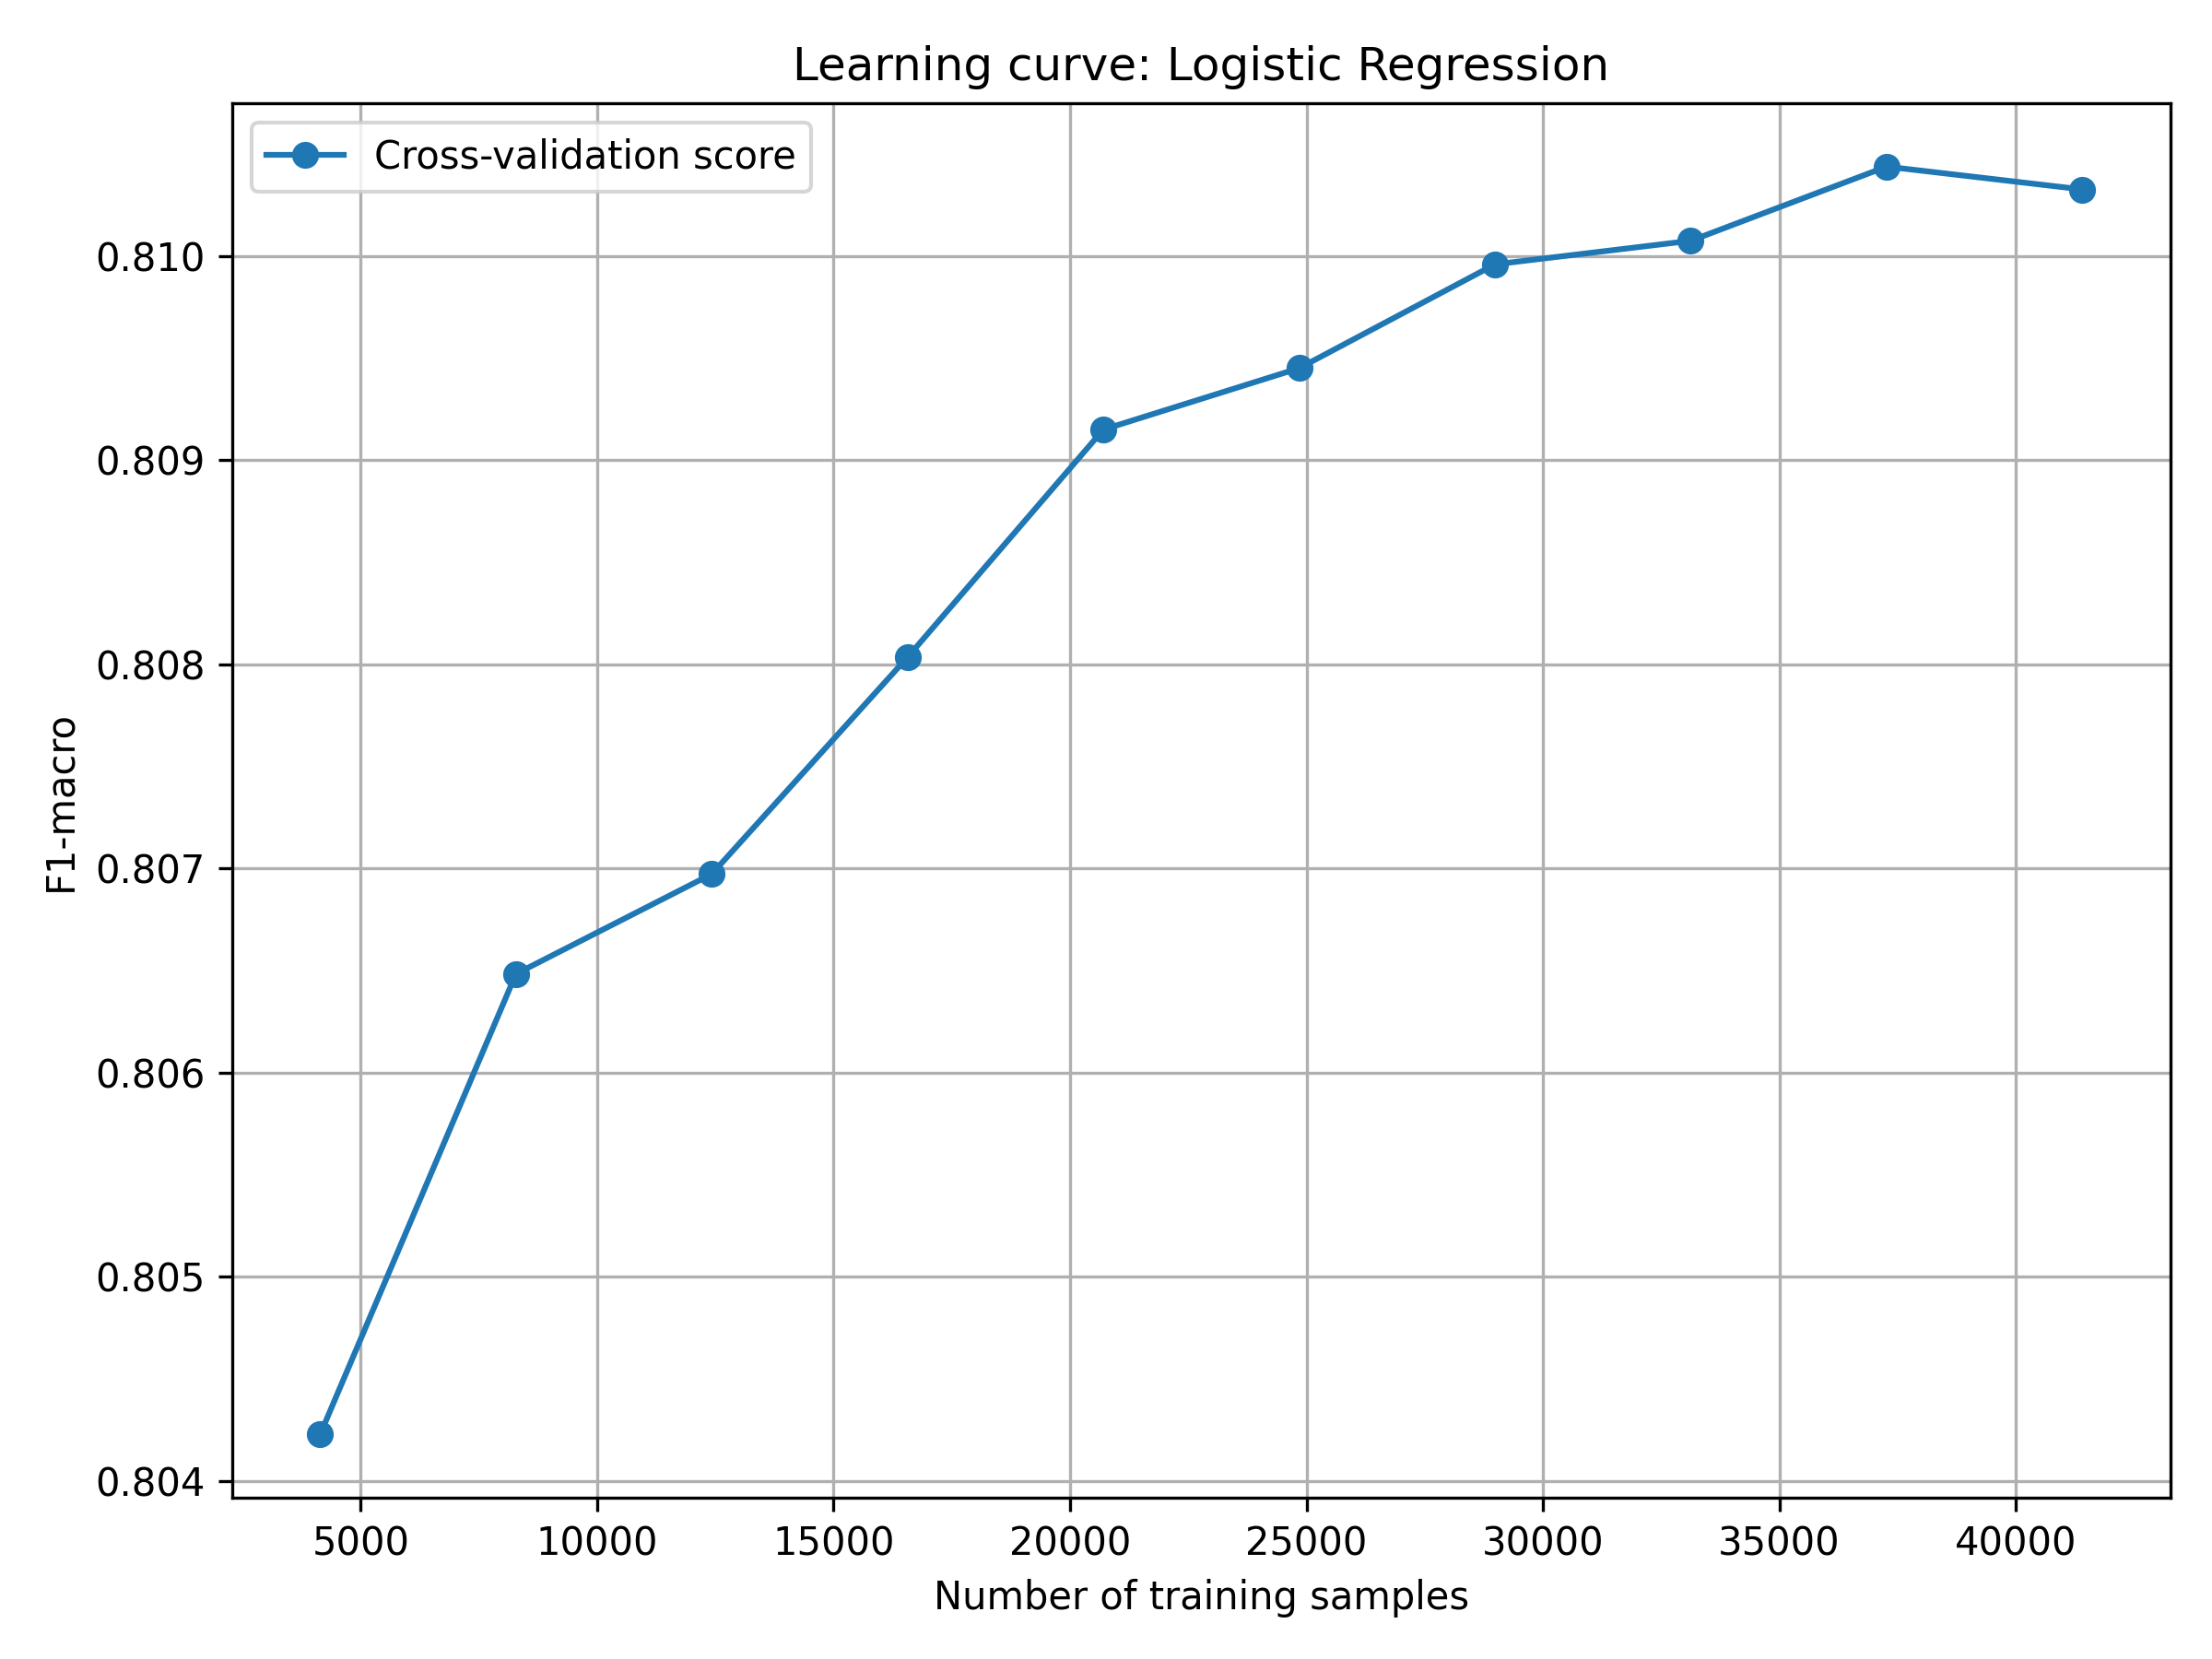
\includegraphics[width=0.82\textwidth]{logistic_regression_images/logistic_regression_learning_curve.png}
\caption{Кривая обучения: Logistic Regression}
\end{figure}
\begin{figure}[H]
\centering
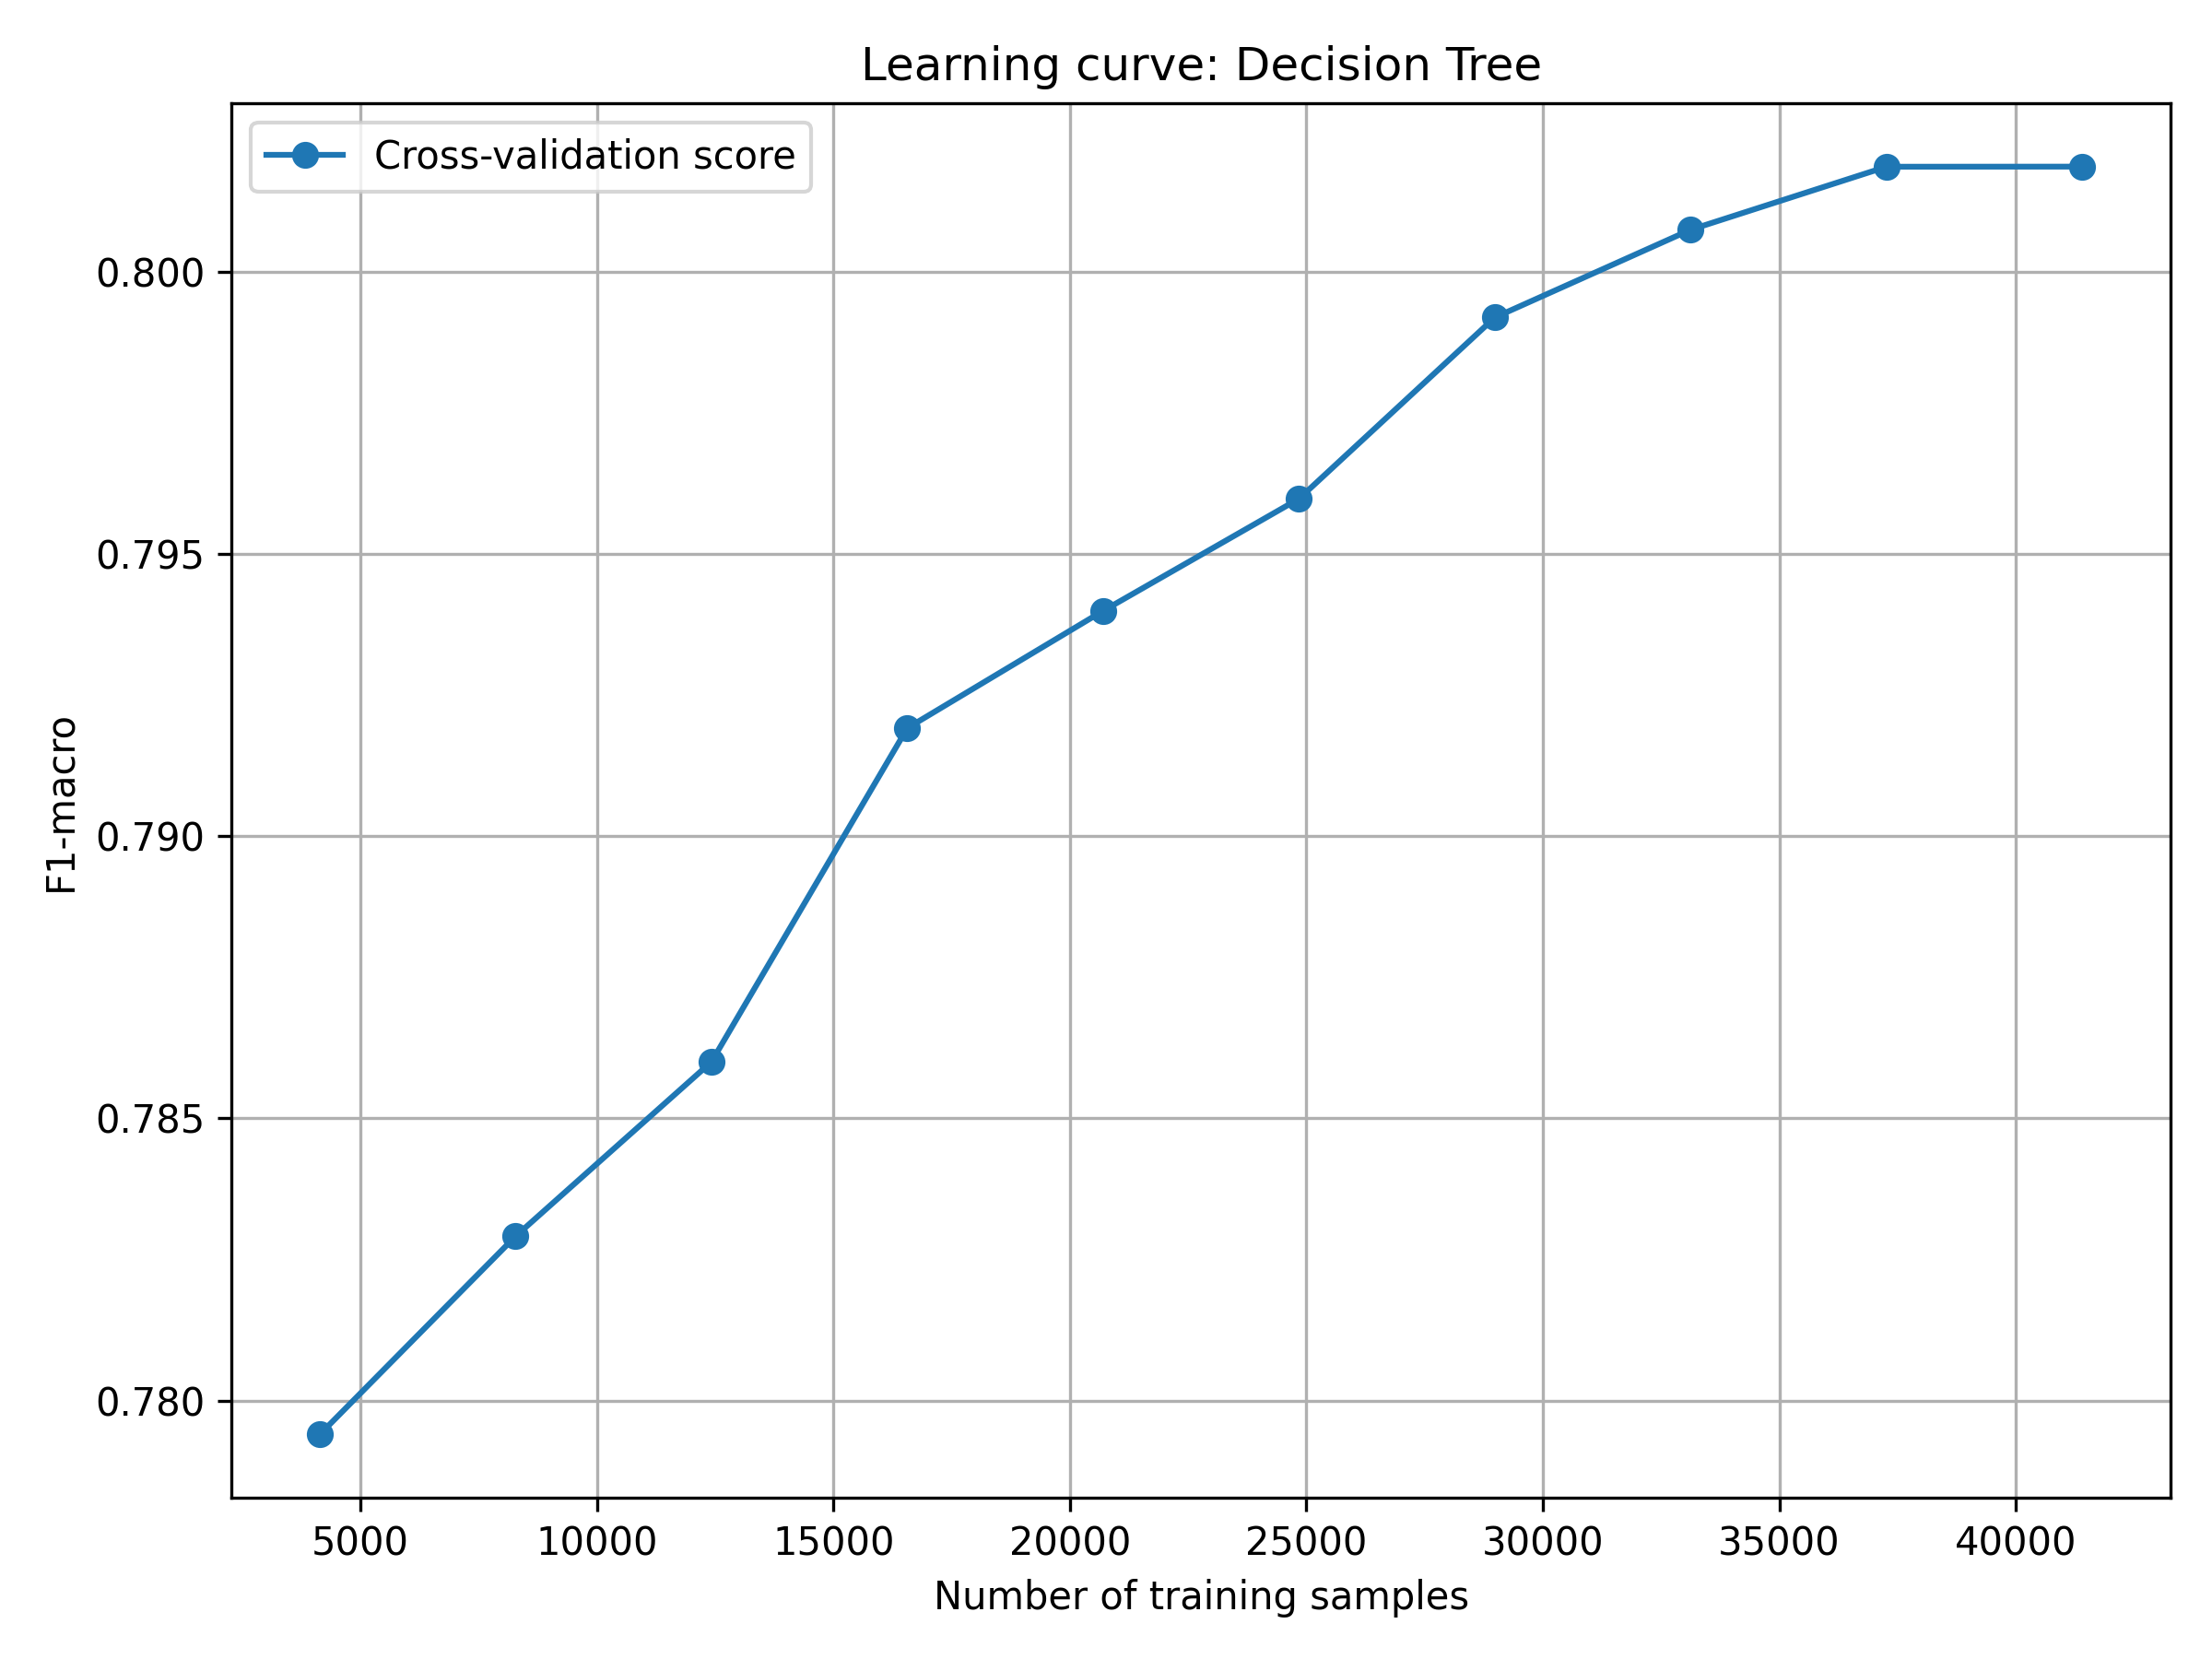
\includegraphics[width=0.82\textwidth]{decision_tree_images/decision_tree_learning_curve.png}
\caption{Кривая обучения: Decision Tree}
\end{figure}
\begin{figure}[H]
\centering
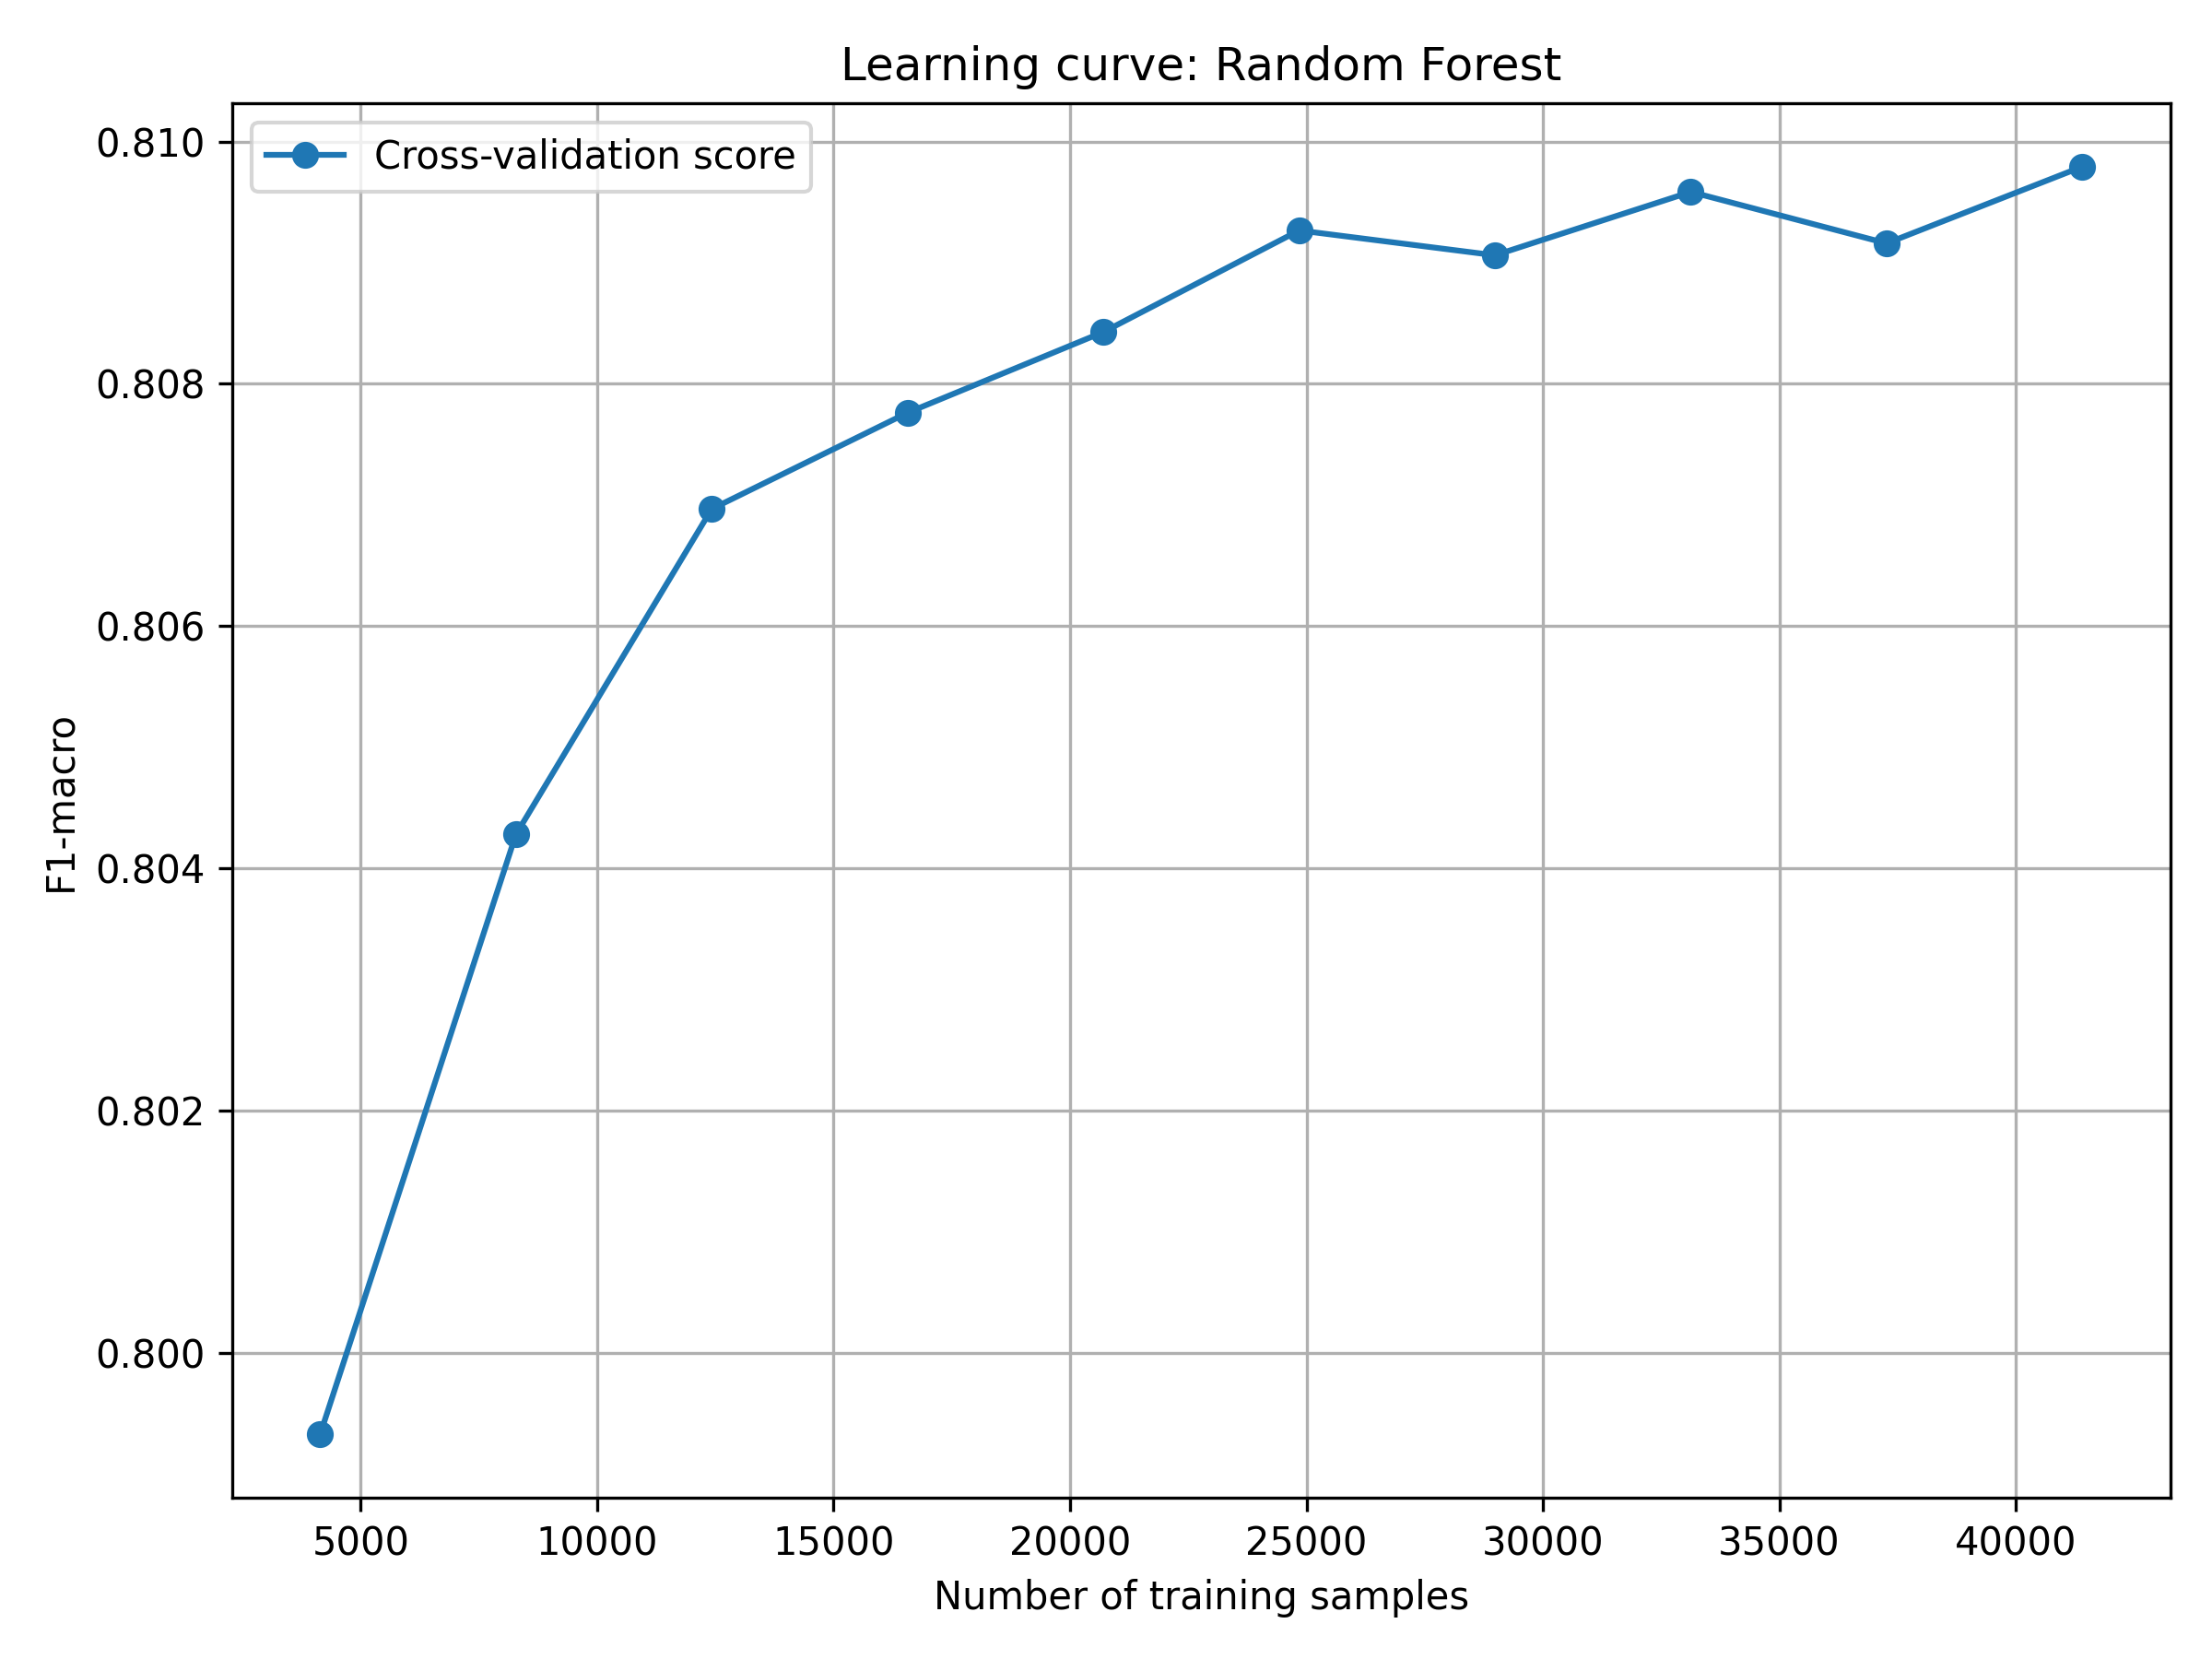
\includegraphics[width=0.82\textwidth]{random_forest_images/random_forest_learning_curve.png}
\caption{Кривая обучения: Random Forest}
\end{figure}
\begin{figure}[H]
\centering
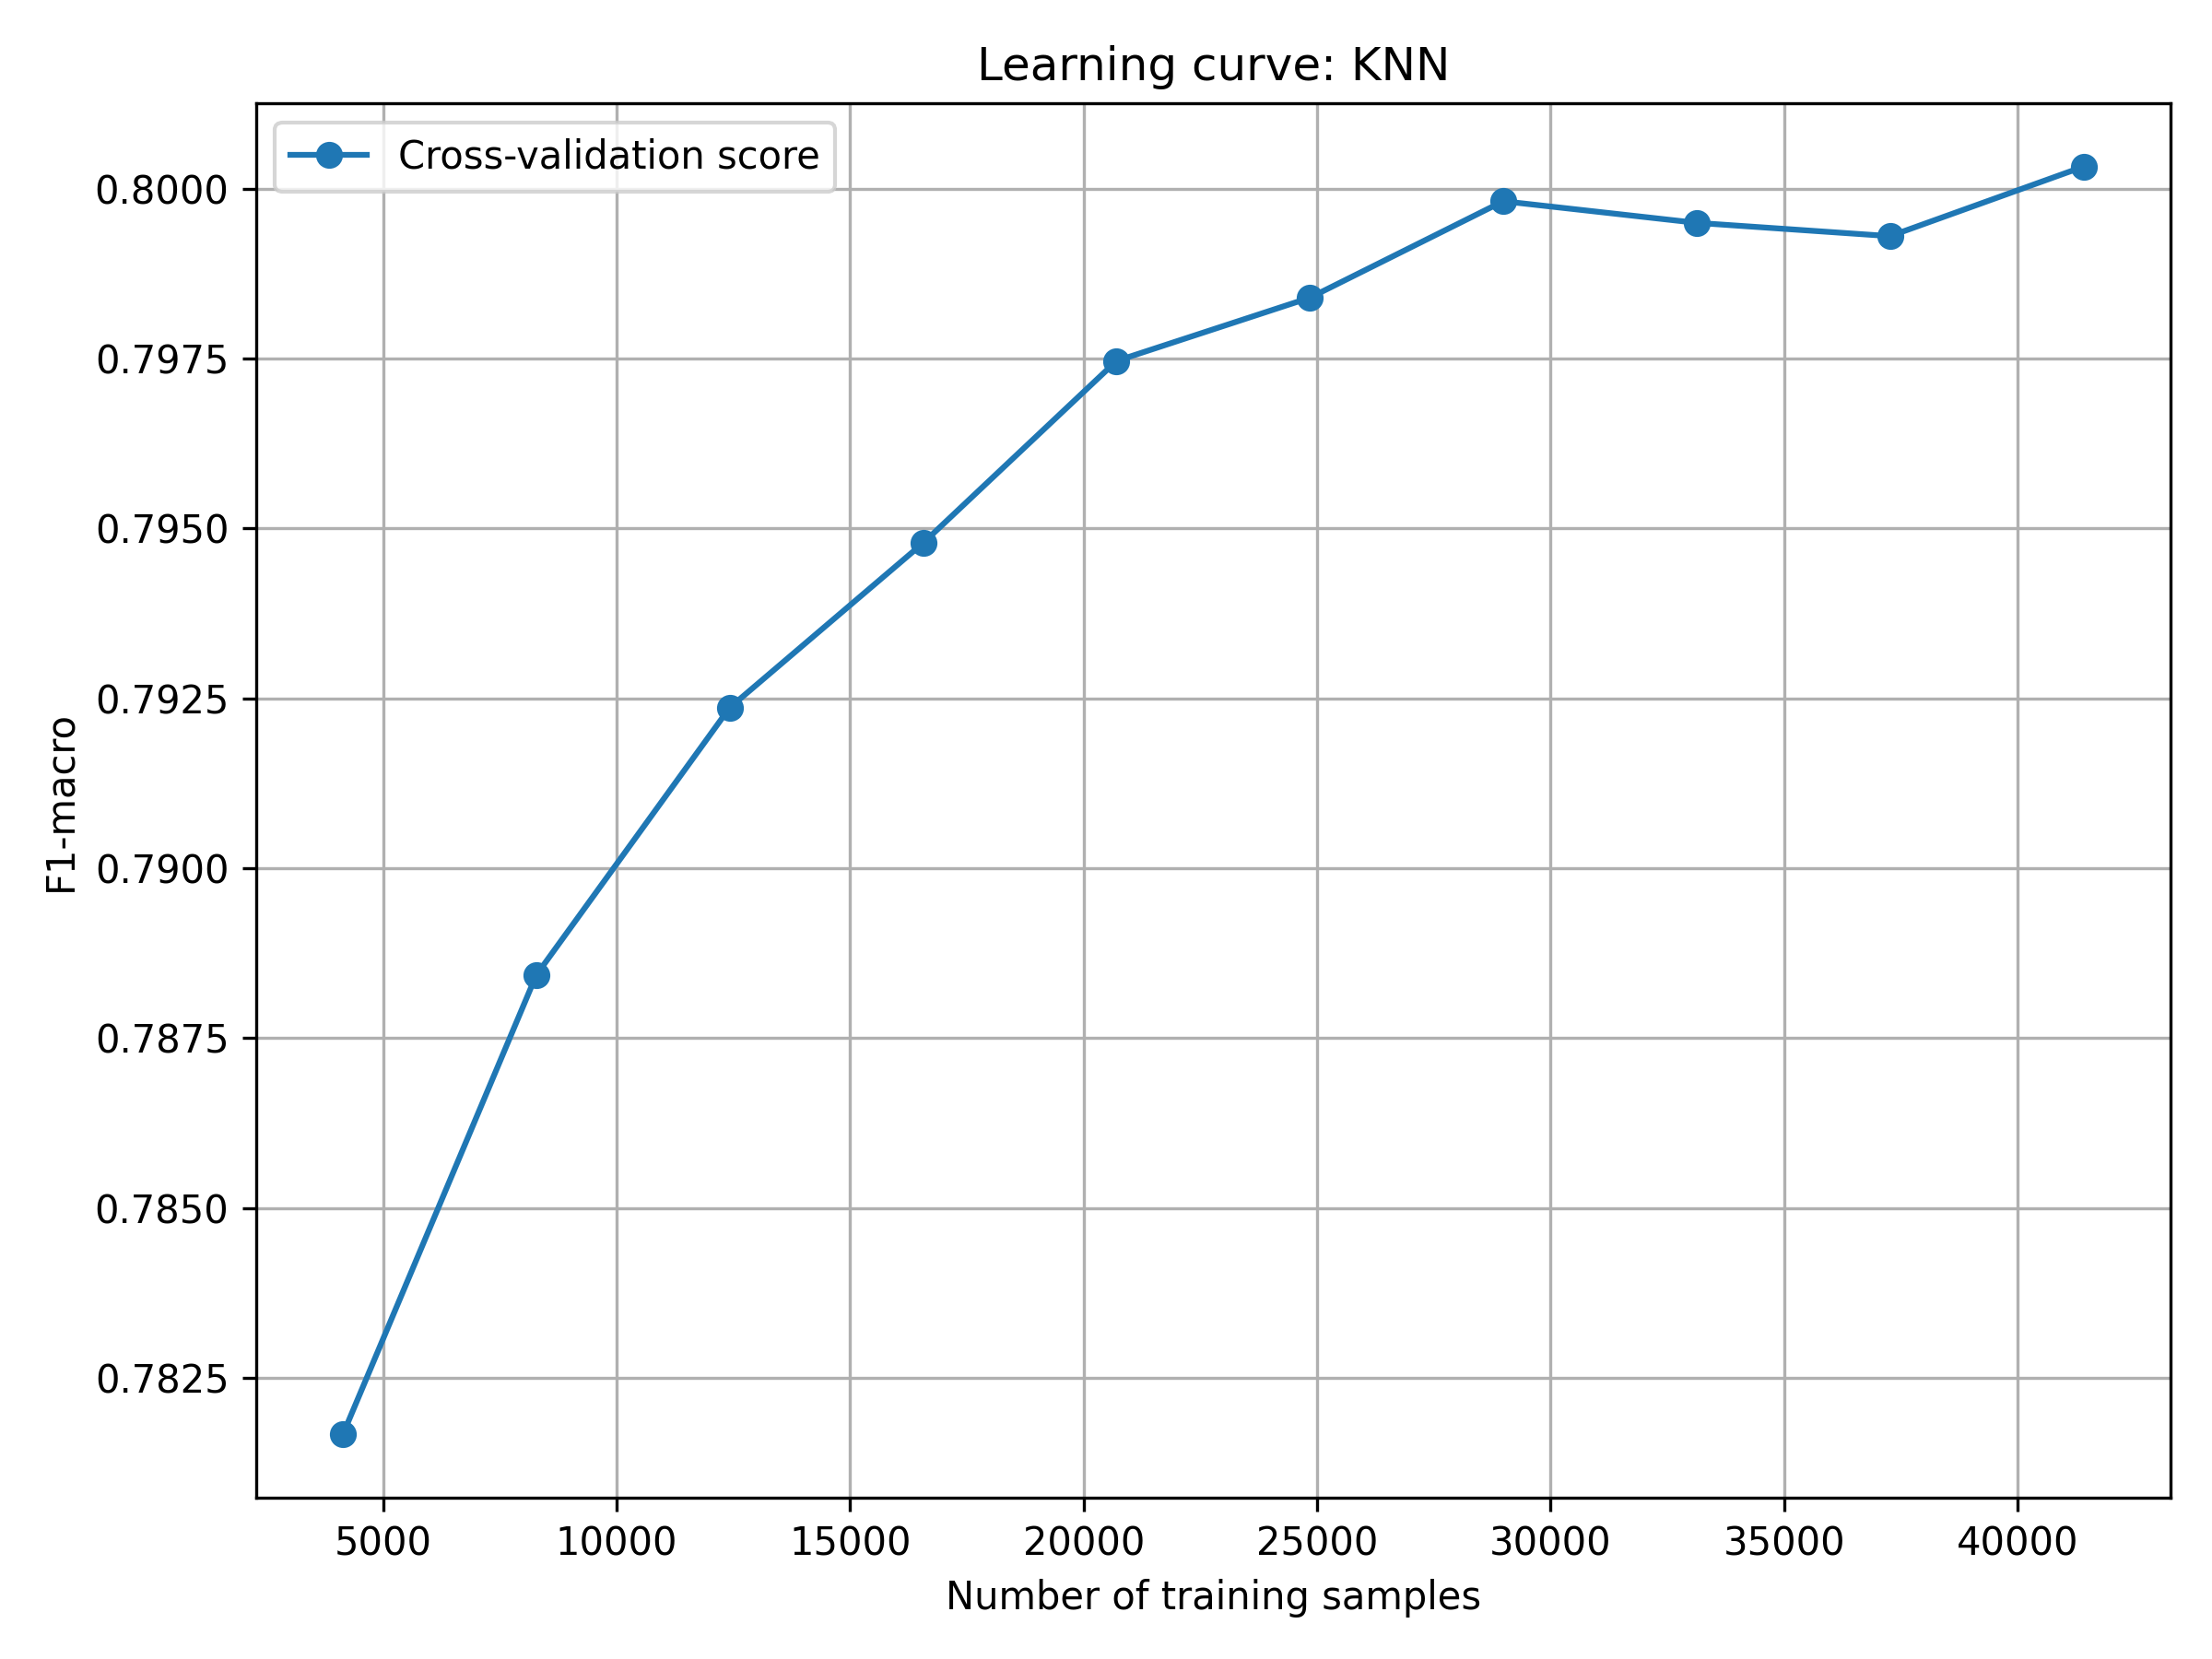
\includegraphics[width=0.82\textwidth]{knn_images/knn_learning_curve.png}
\caption{Кривая обучения: KNN}
\end{figure}
\begin{figure}[H]
\centering
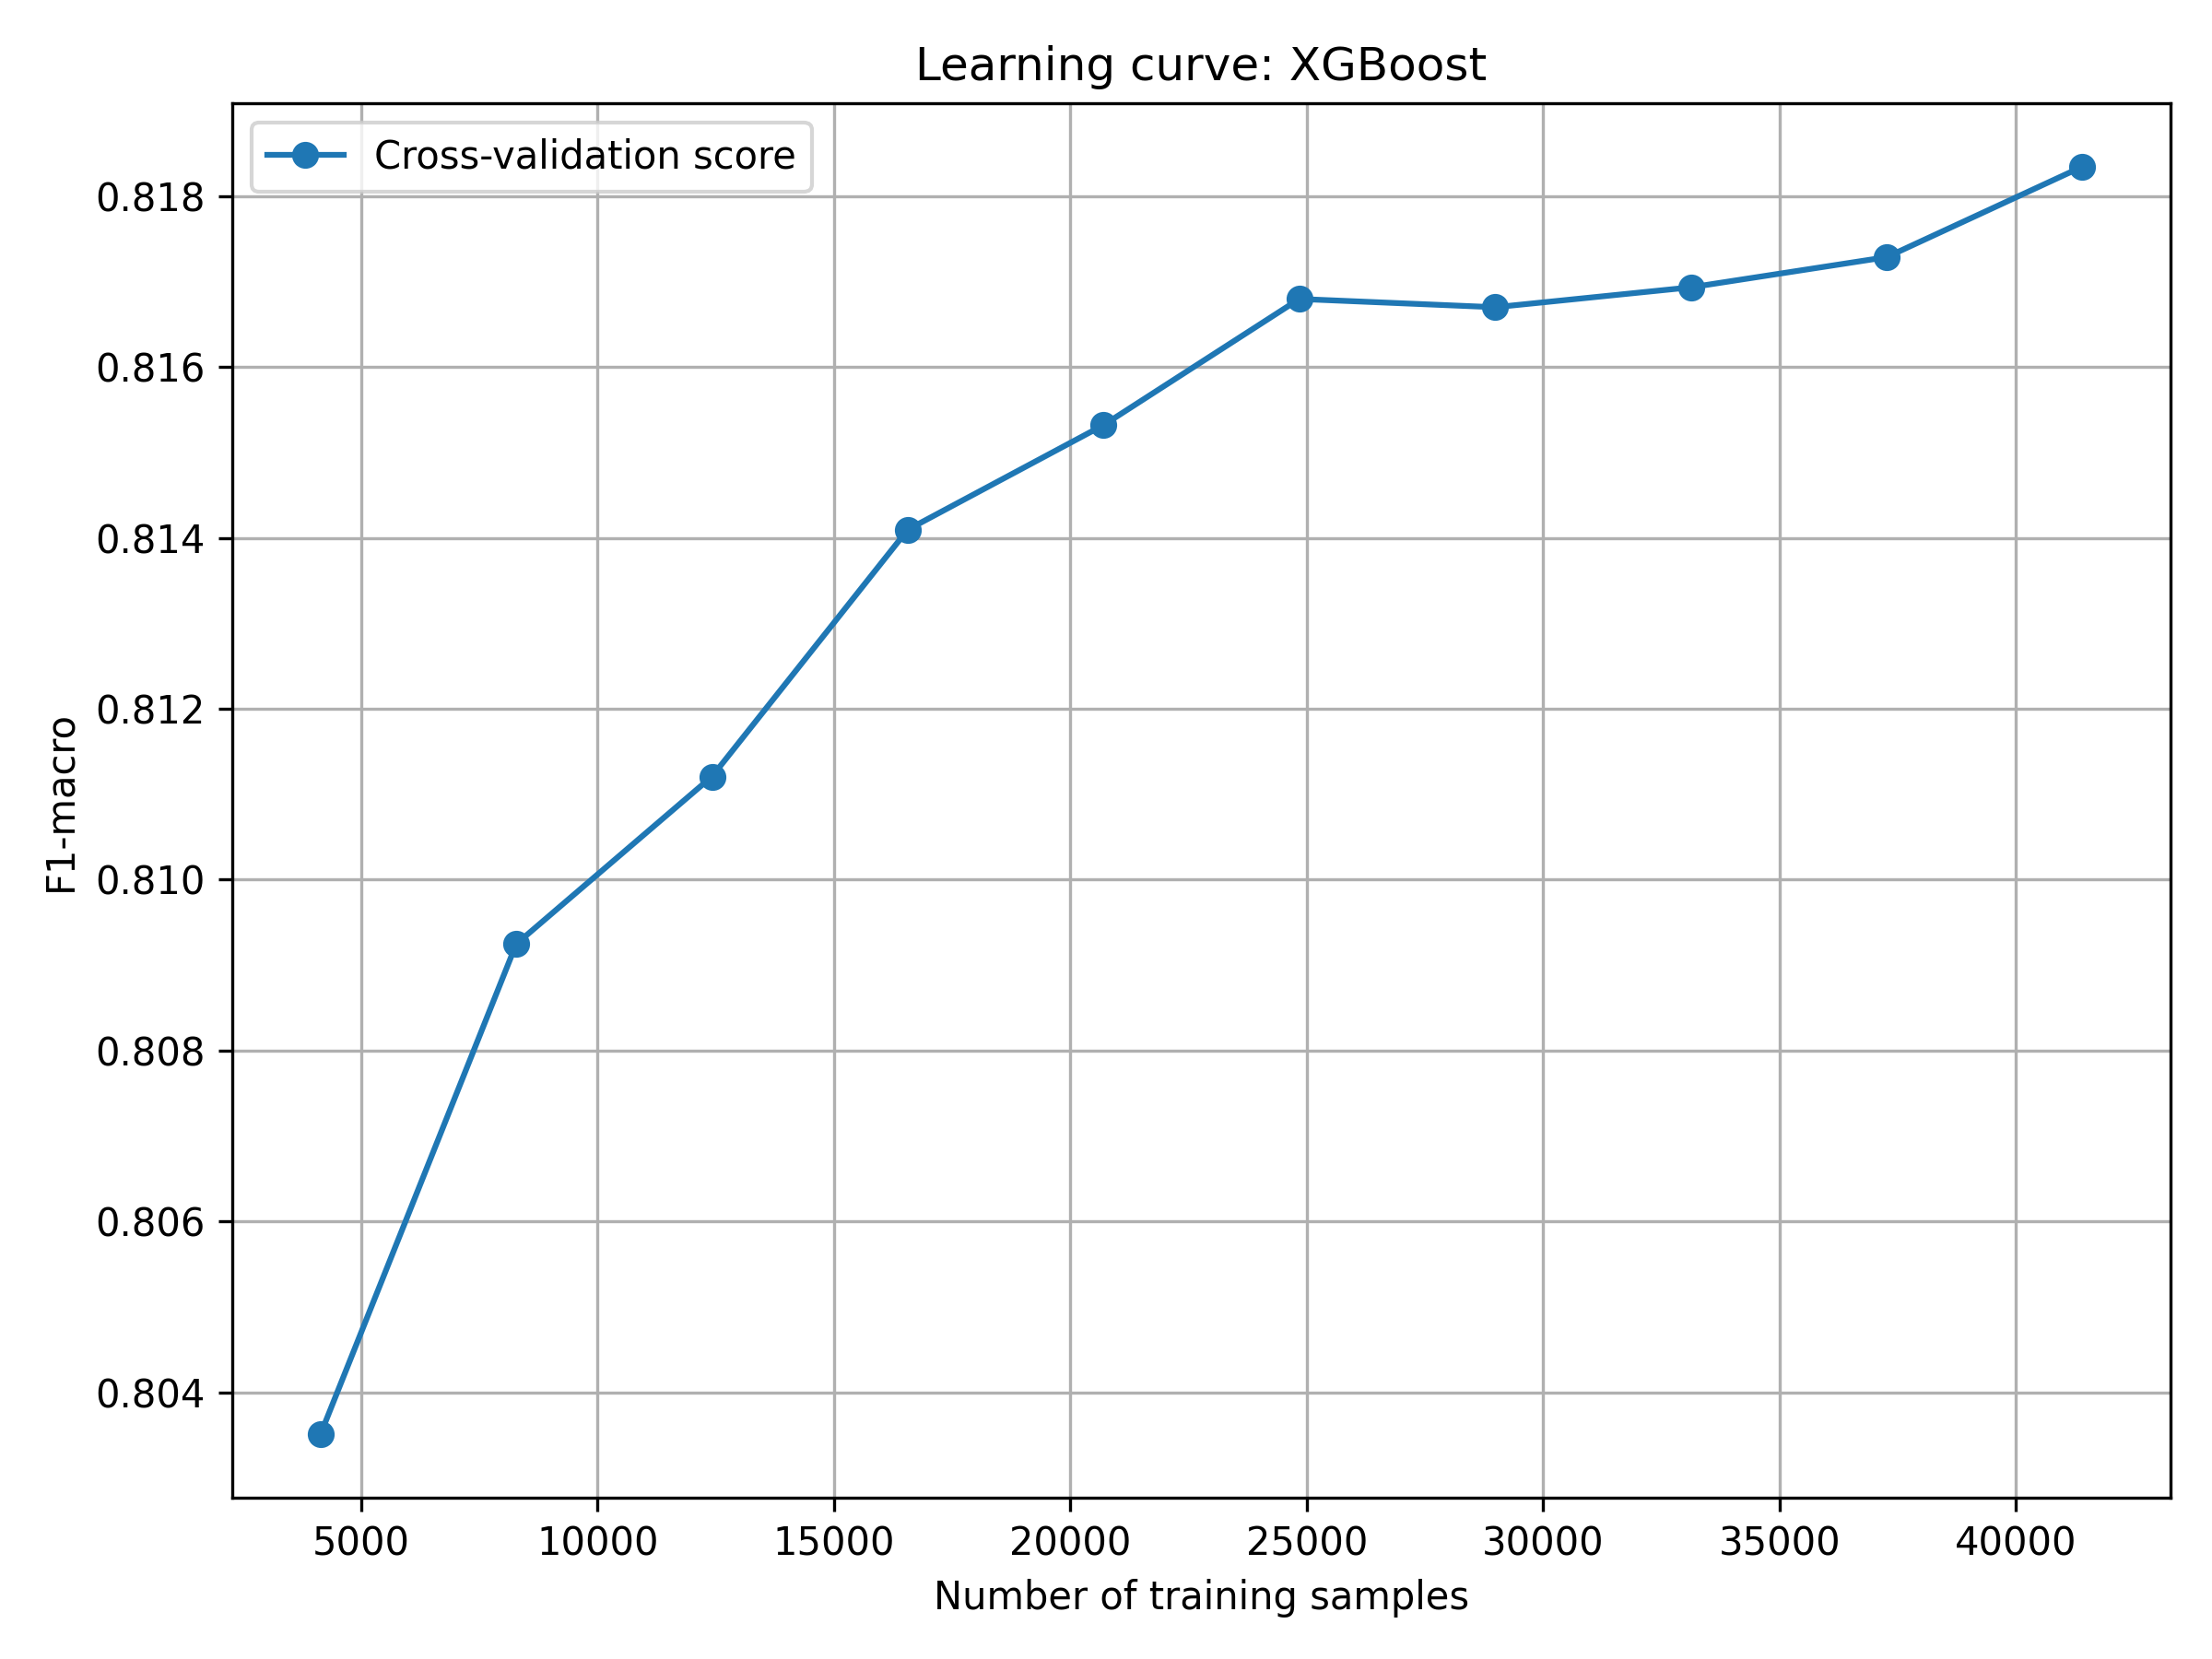
\includegraphics[width=0.82\textwidth]{xgboost_images/xgboost_learning_curve.png}
\caption{Кривая обучения: XGBoost}
\end{figure}
\begin{figure}[H]
\centering
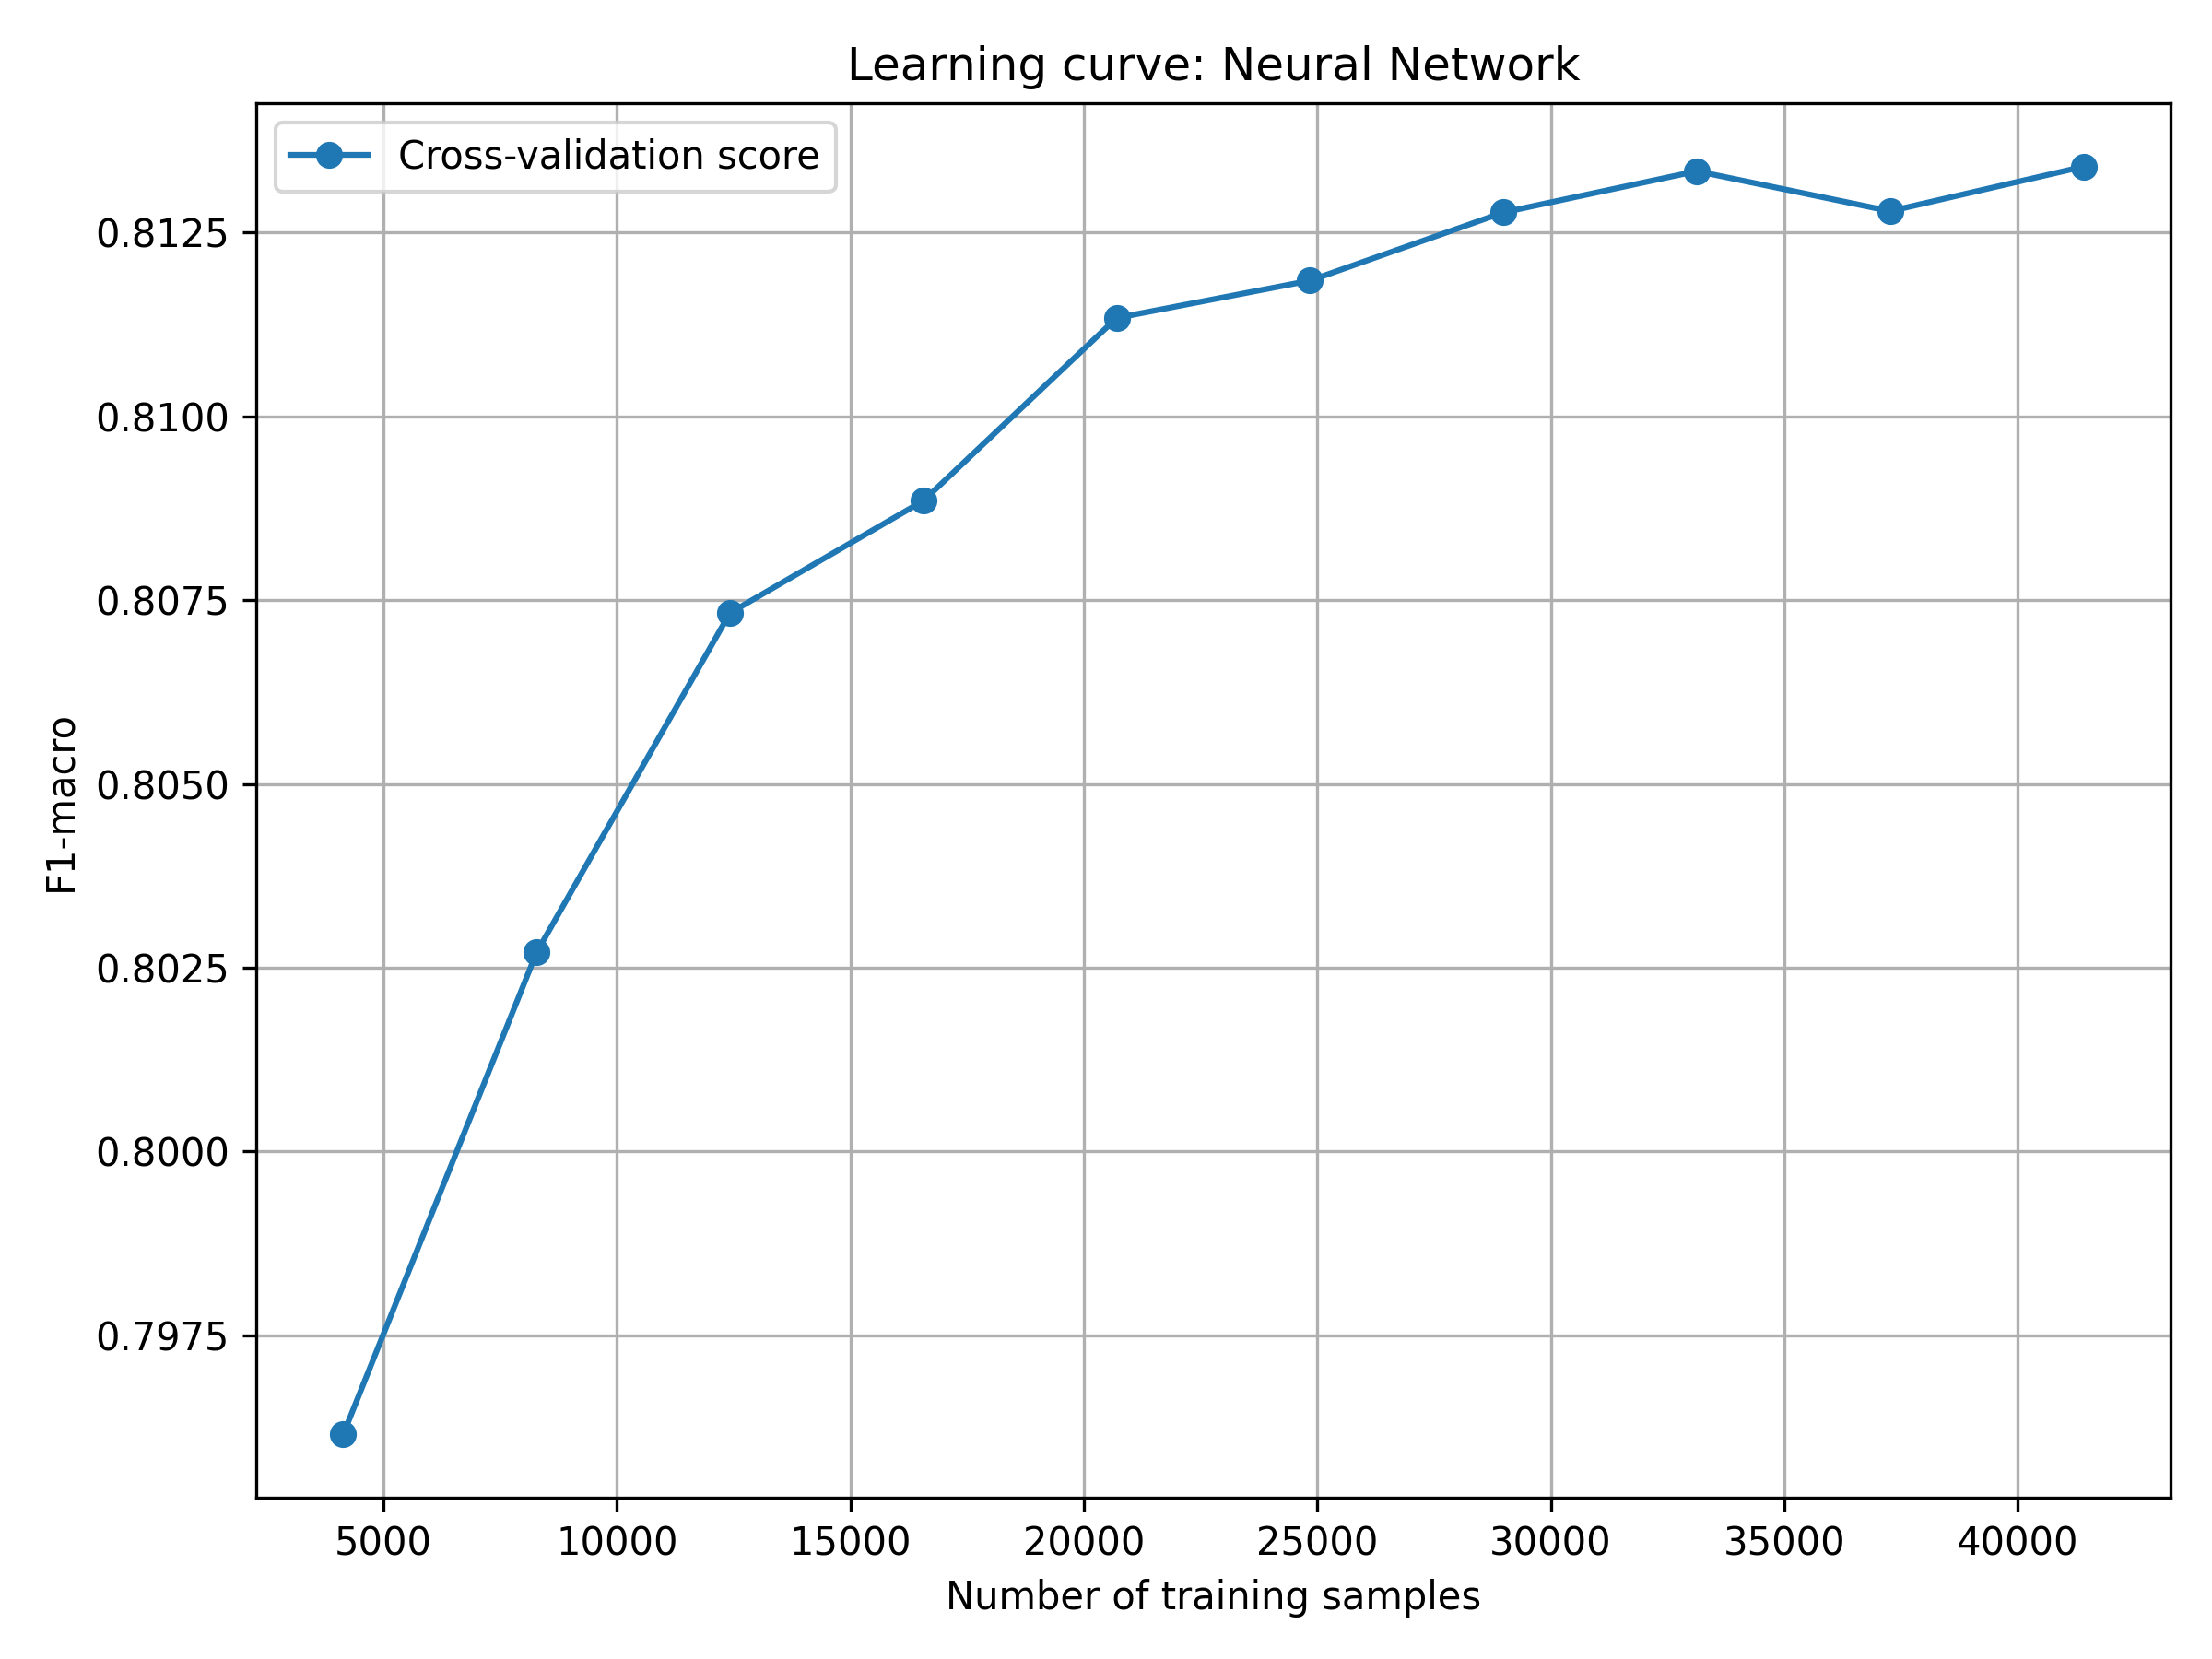
\includegraphics[width=0.82\textwidth]{neural_network_images/neural_network_learning_curve.png}
\caption{Кривая обучения: Neural Network}
\end{figure}

Кривые обучения позволяют оценить, выигрывает ли модель от увеличения объема обучающих данных и насколько велик разрыв между train- и validation-качеством. Для XGBoost и Random Forest заметен более высокий train F1, что указывает на большую емкость ансамблей. При этом validation F1 у XGBoost продолжает расти при увеличении обучающей выборки, поэтому модель выигрывает от дополнительного объема данных. Для логистической регрессии разрыв между train и validation меньше, что характерно для регуляризованной линейной модели. Decision Tree и KNN имеют более низкий итоговый validation F1: одиночному дереву не хватает устойчивости ансамбля, а KNN хуже использует высокоразмерное пространство после one-hot encoding.

\section{Анализ справедливости модели}

\scriptsize
\begin{longtable}{lllll}
\caption{Наибольшие разрывы качества между группами}\label{tab:fairness_gaps}\\
\toprule
Модель & Атрибут & F1 gap & Error rate gap & Recall positive gap \\
\midrule
\endfirsthead
\toprule
Модель & Атрибут & F1 gap & Error rate gap & Recall positive gap \\
\midrule
\endhead
Logistic Regression & trip\_purpose & 0.141 & 0.142 & 0.103 \\
Logistic Regression & age\_group & 0.094 & 0.089 & 0.125 \\
Logistic Regression & process & 0.072 & 0.067 & 0.024 \\
Decision Tree & trip\_purpose & 0.129 & 0.130 & 0.114 \\
Decision Tree & age\_group & 0.085 & 0.083 & 0.085 \\
Decision Tree & process & 0.064 & 0.060 & 0.037 \\
Random Forest & trip\_purpose & 0.148 & 0.147 & 0.138 \\
Random Forest & age\_group & 0.091 & 0.089 & 0.089 \\
Random Forest & process & 0.080 & 0.075 & 0.043 \\
KNN & age\_group & 0.085 & 0.085 & 0.101 \\
KNN & trip\_purpose & 0.083 & 0.079 & 0.089 \\
KNN & process & 0.066 & 0.061 & 0.064 \\
XGBoost & trip\_purpose & 0.153 & 0.153 & 0.172 \\
XGBoost & age\_group & 0.094 & 0.090 & 0.092 \\
XGBoost & process & 0.085 & 0.081 & 0.025 \\
Neural Network & trip\_purpose & 0.138 & 0.140 & 0.079 \\
Neural Network & age\_group & 0.092 & 0.089 & 0.121 \\
Neural Network & process & 0.073 & 0.071 & 0.007 \\
\bottomrule
\end{longtable}
\normalsize
\begin{figure}[H]
\centering
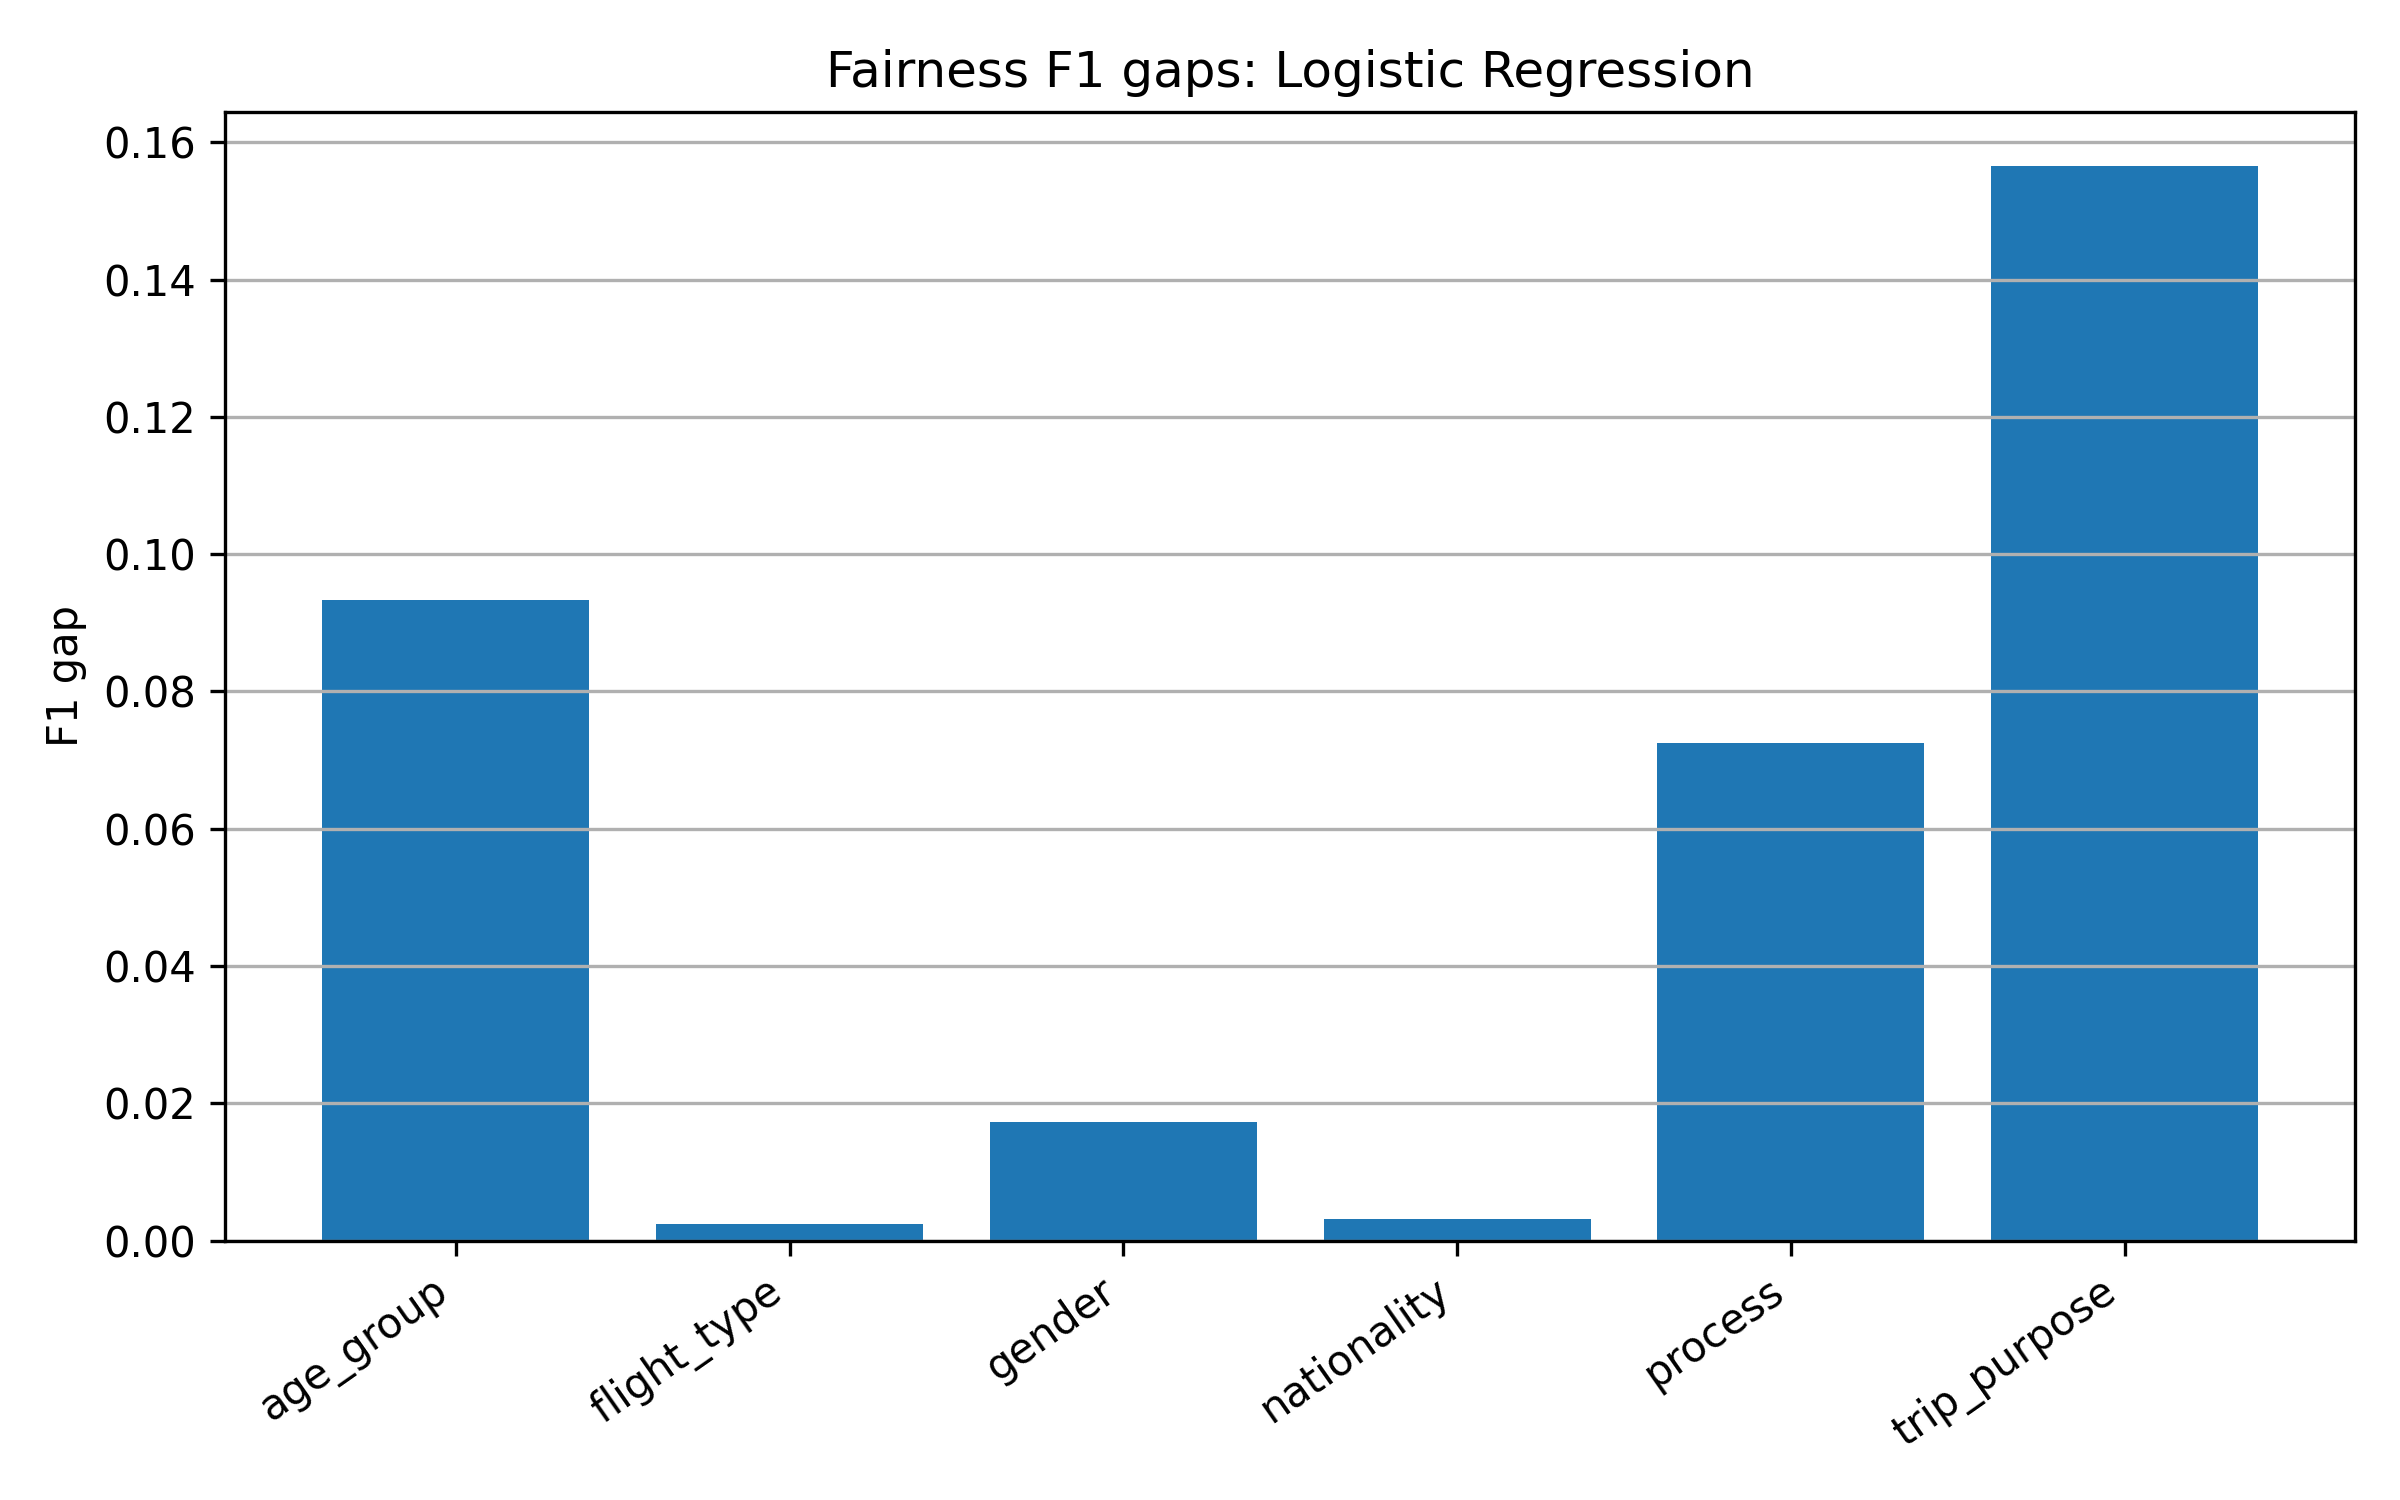
\includegraphics[width=0.82\textwidth]{logistic_regression_images/logistic_regression_fairness_f1_gaps.png}
\caption{Fairness gaps по F1-macro: Logistic Regression}
\end{figure}
\begin{figure}[H]
\centering
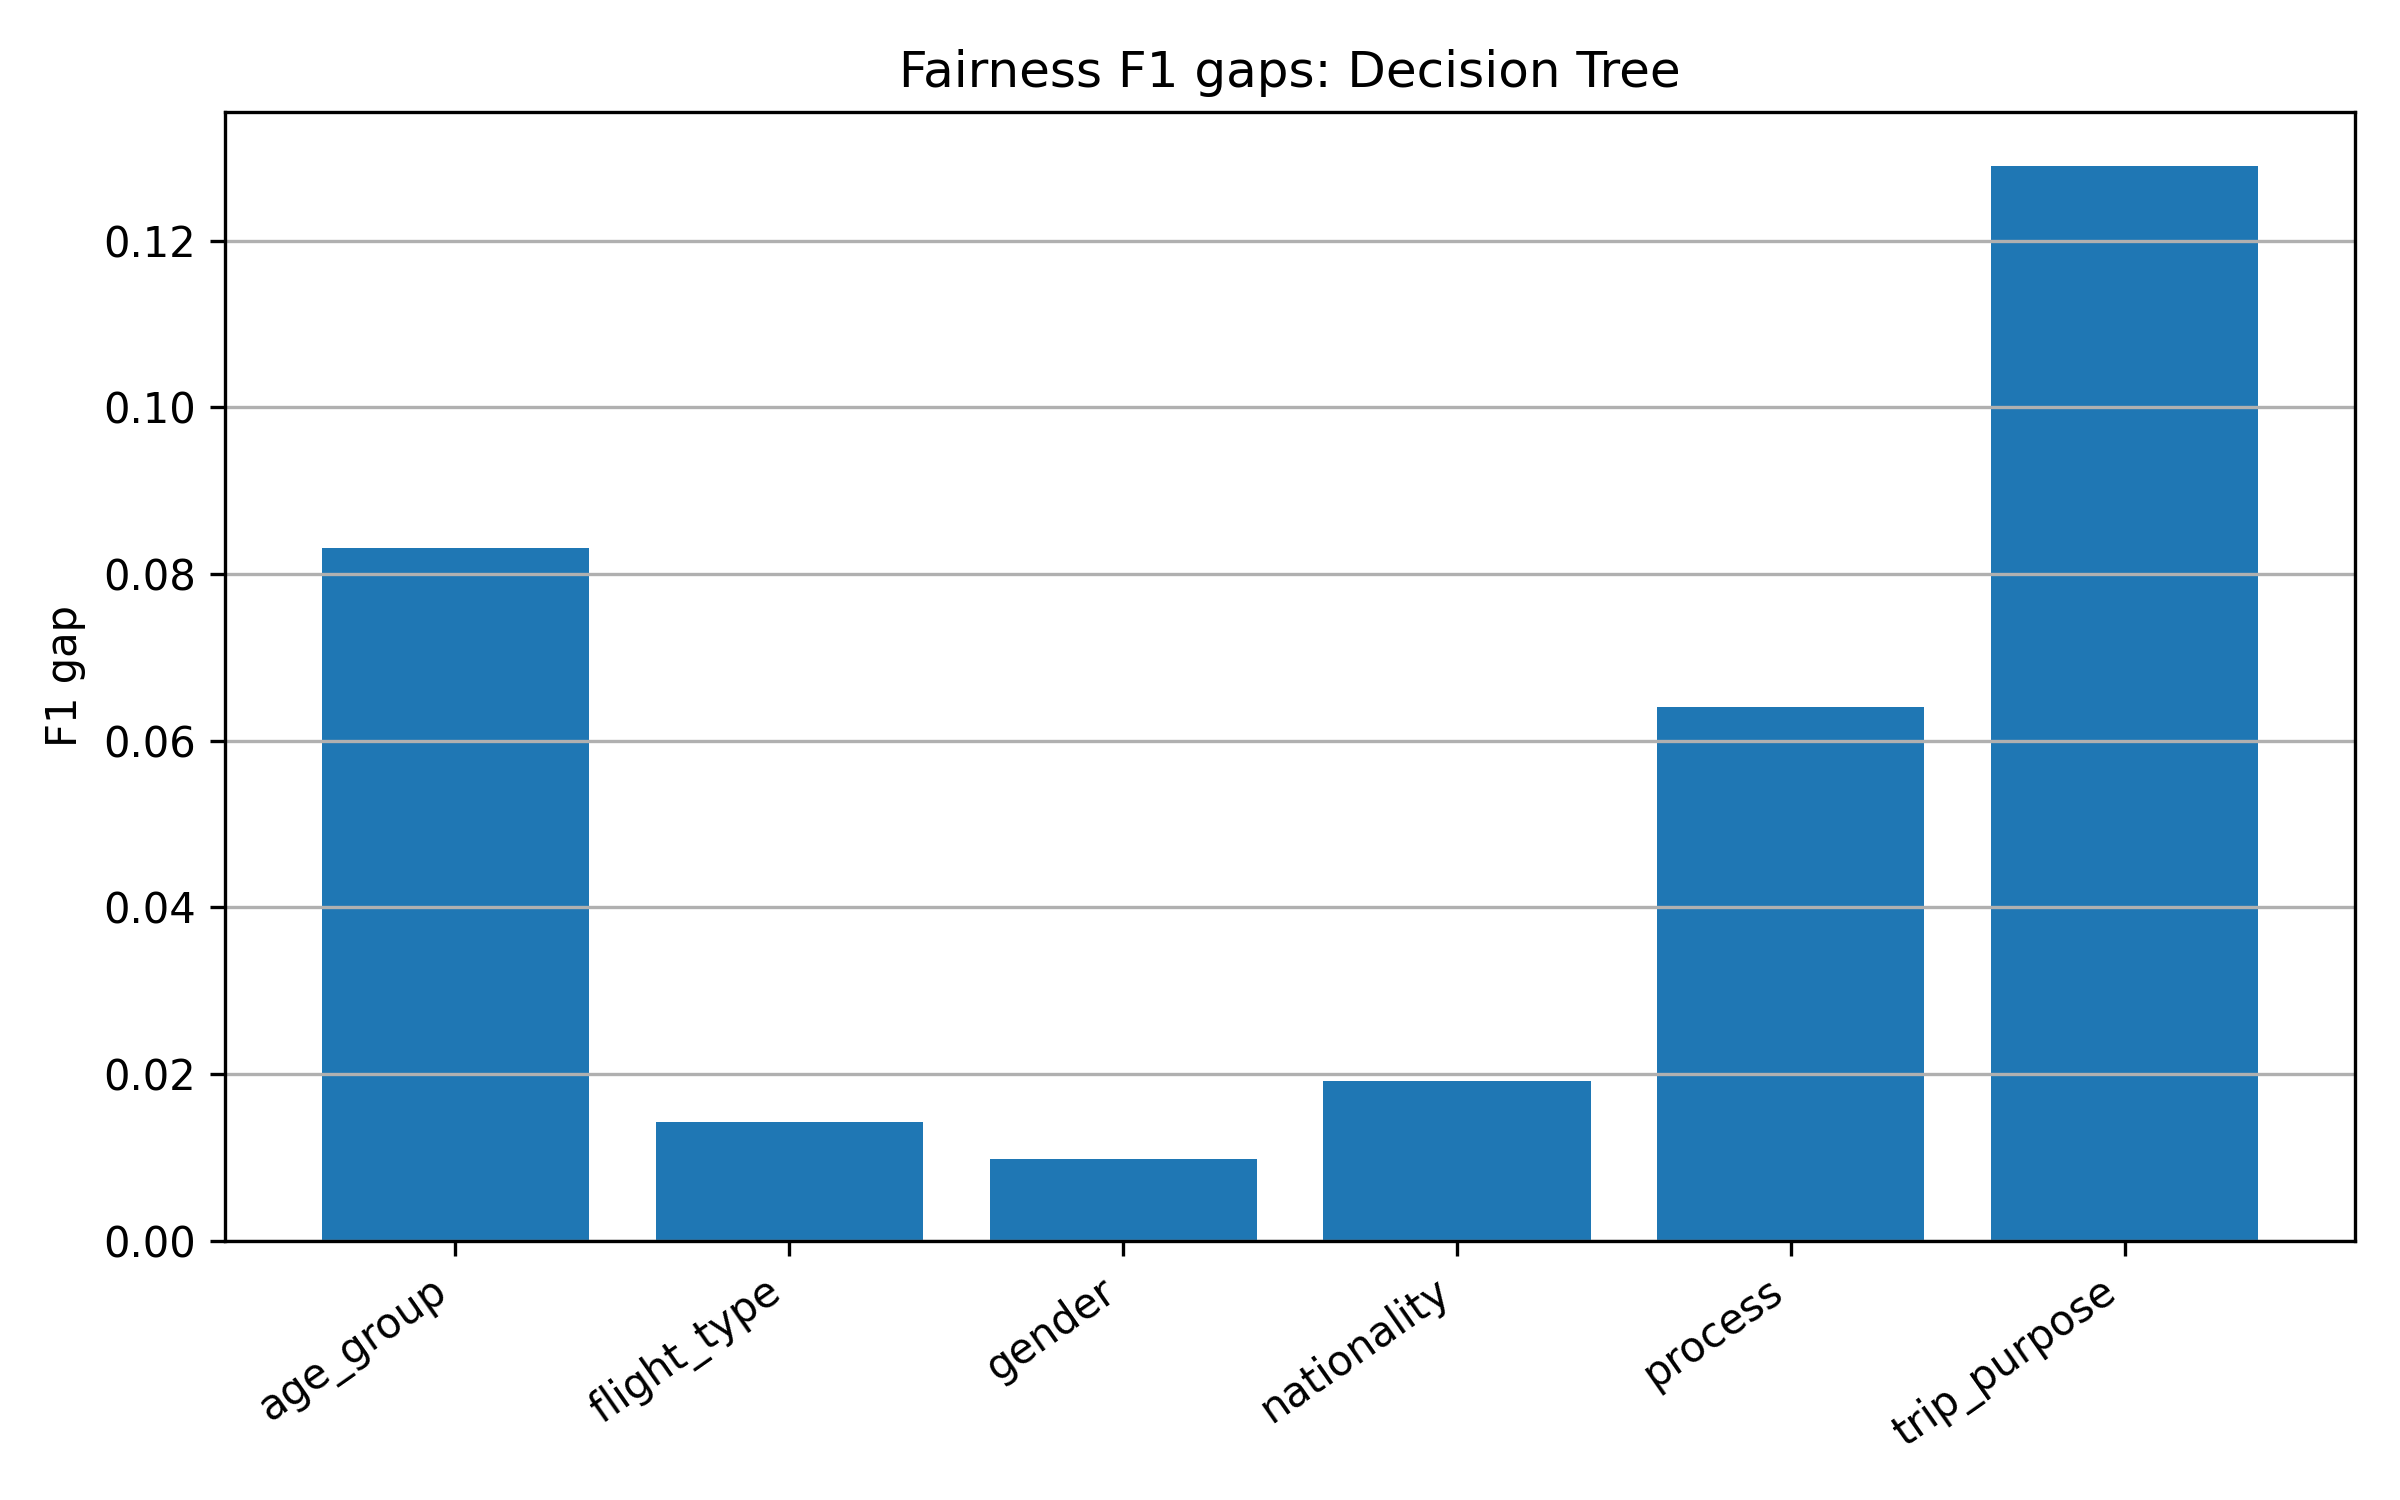
\includegraphics[width=0.82\textwidth]{decision_tree_images/decision_tree_fairness_f1_gaps.png}
\caption{Fairness gaps по F1-macro: Decision Tree}
\end{figure}
\begin{figure}[H]
\centering
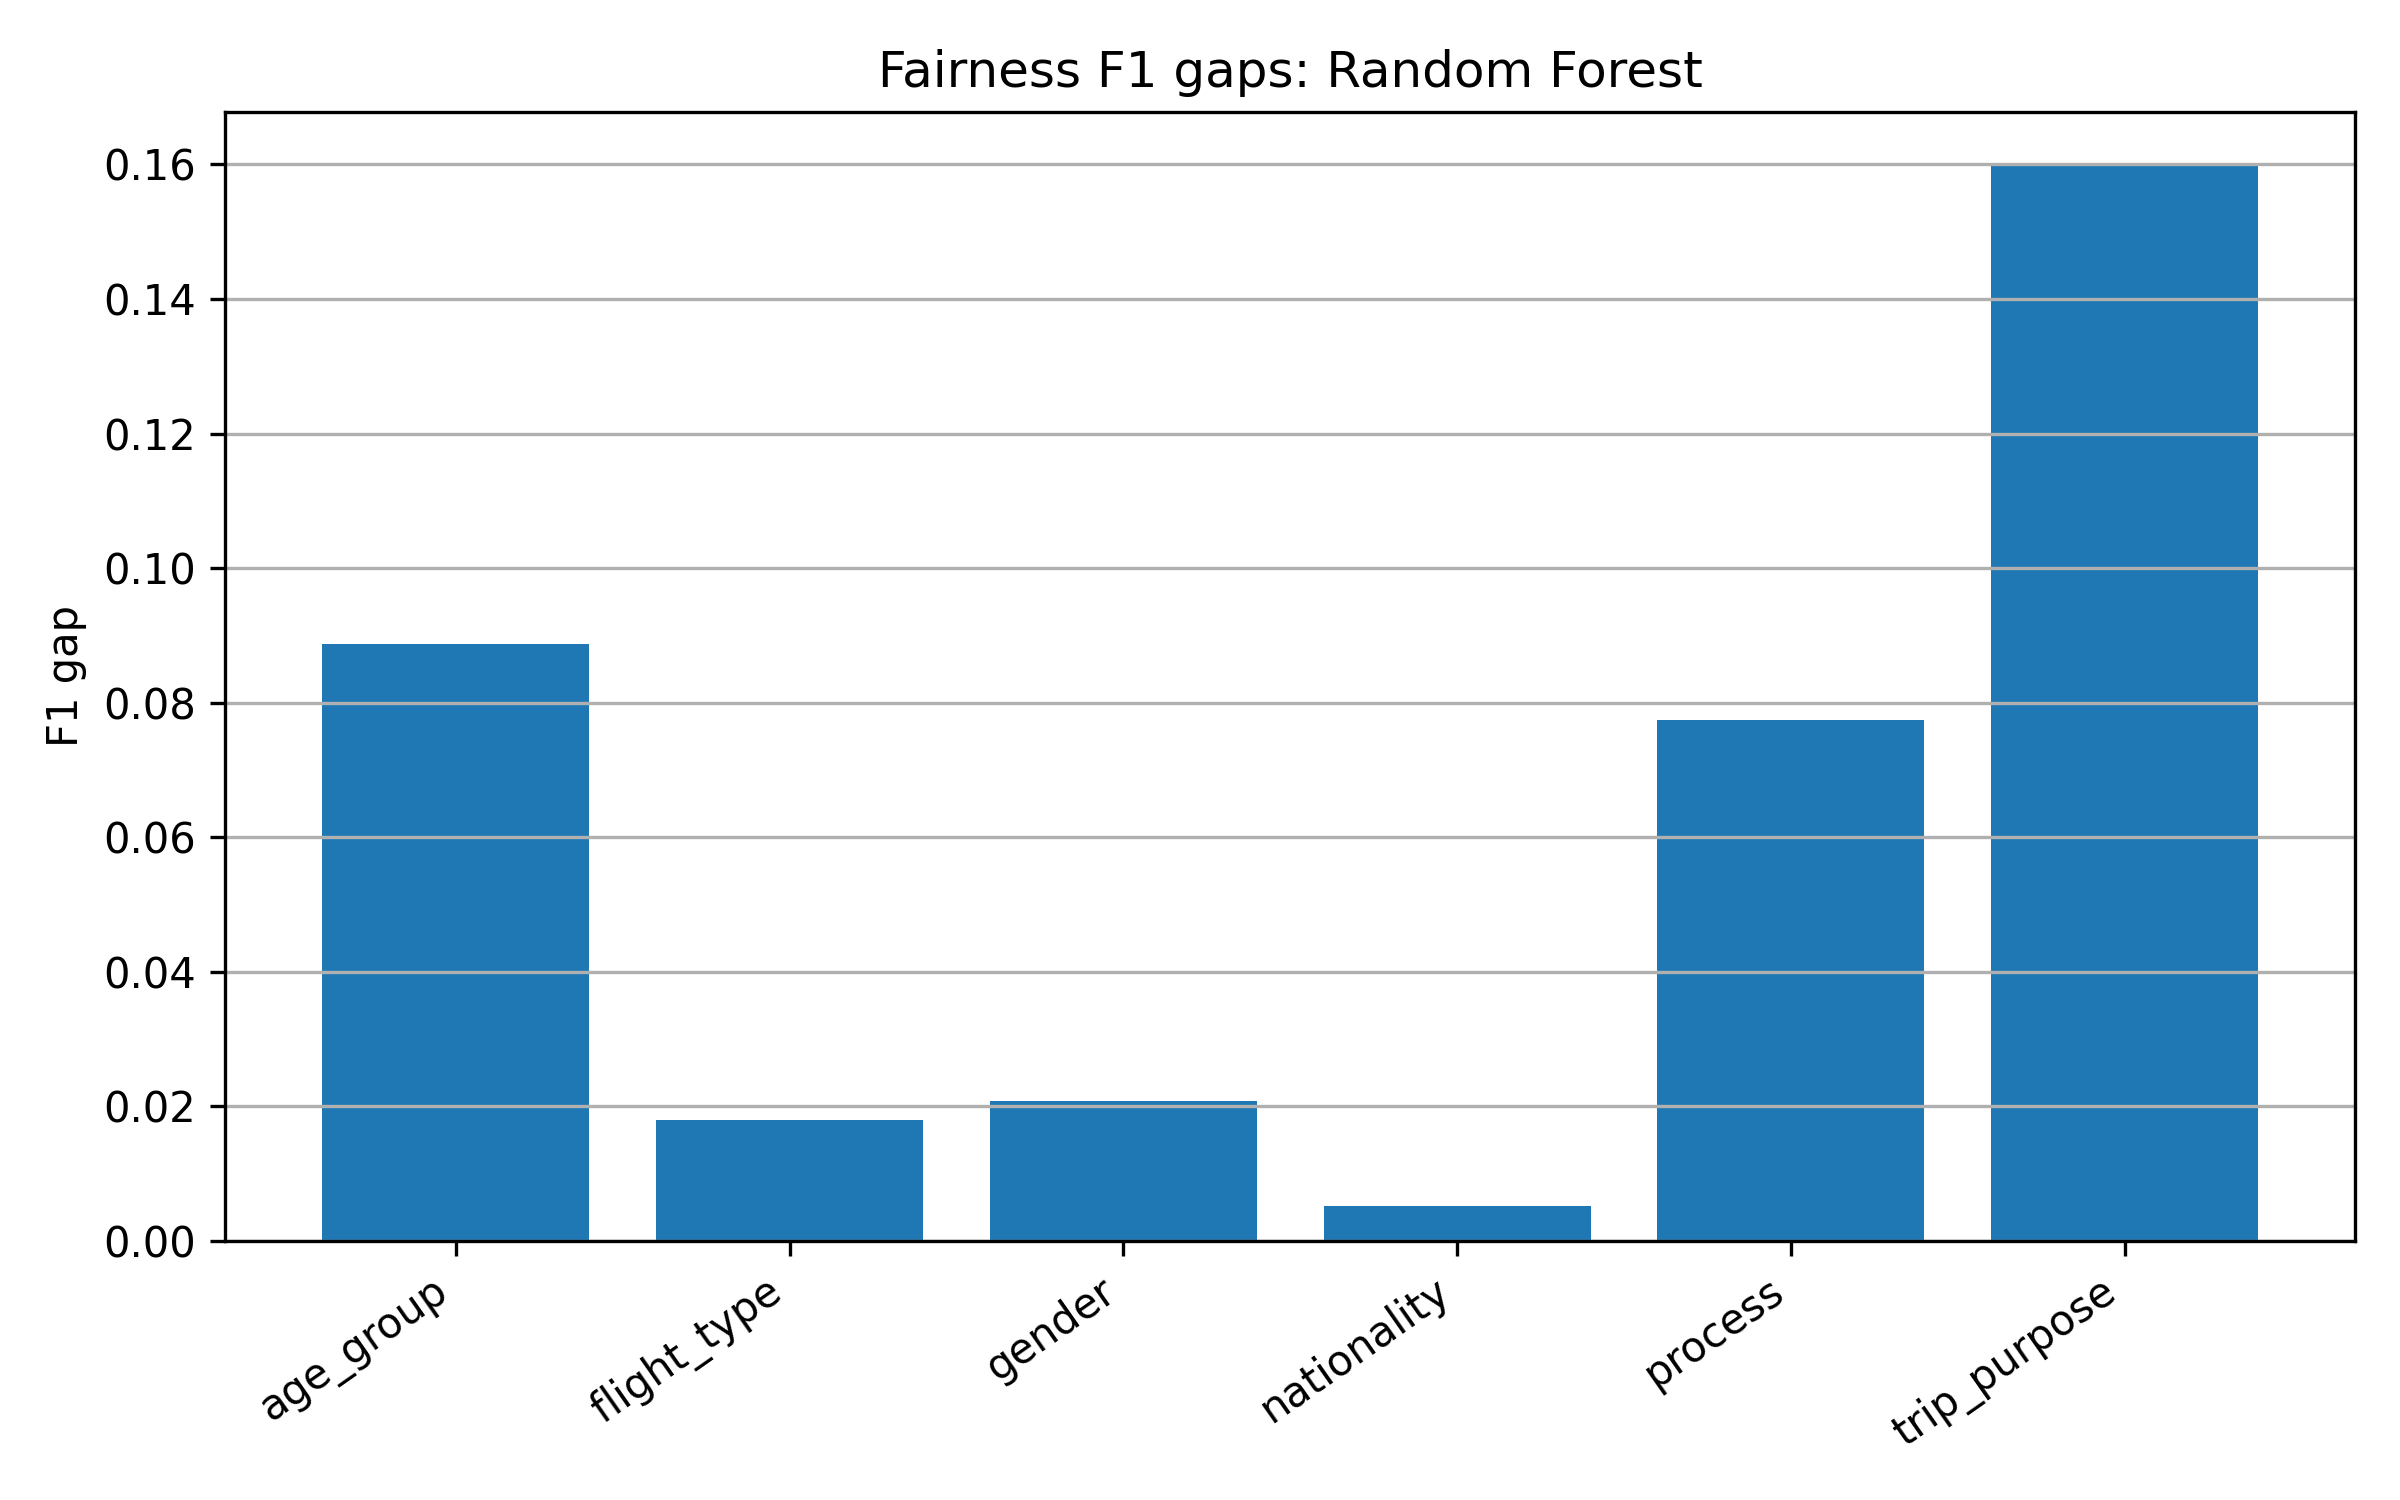
\includegraphics[width=0.82\textwidth]{random_forest_images/random_forest_fairness_f1_gaps.png}
\caption{Fairness gaps по F1-macro: Random Forest}
\end{figure}
\begin{figure}[H]
\centering
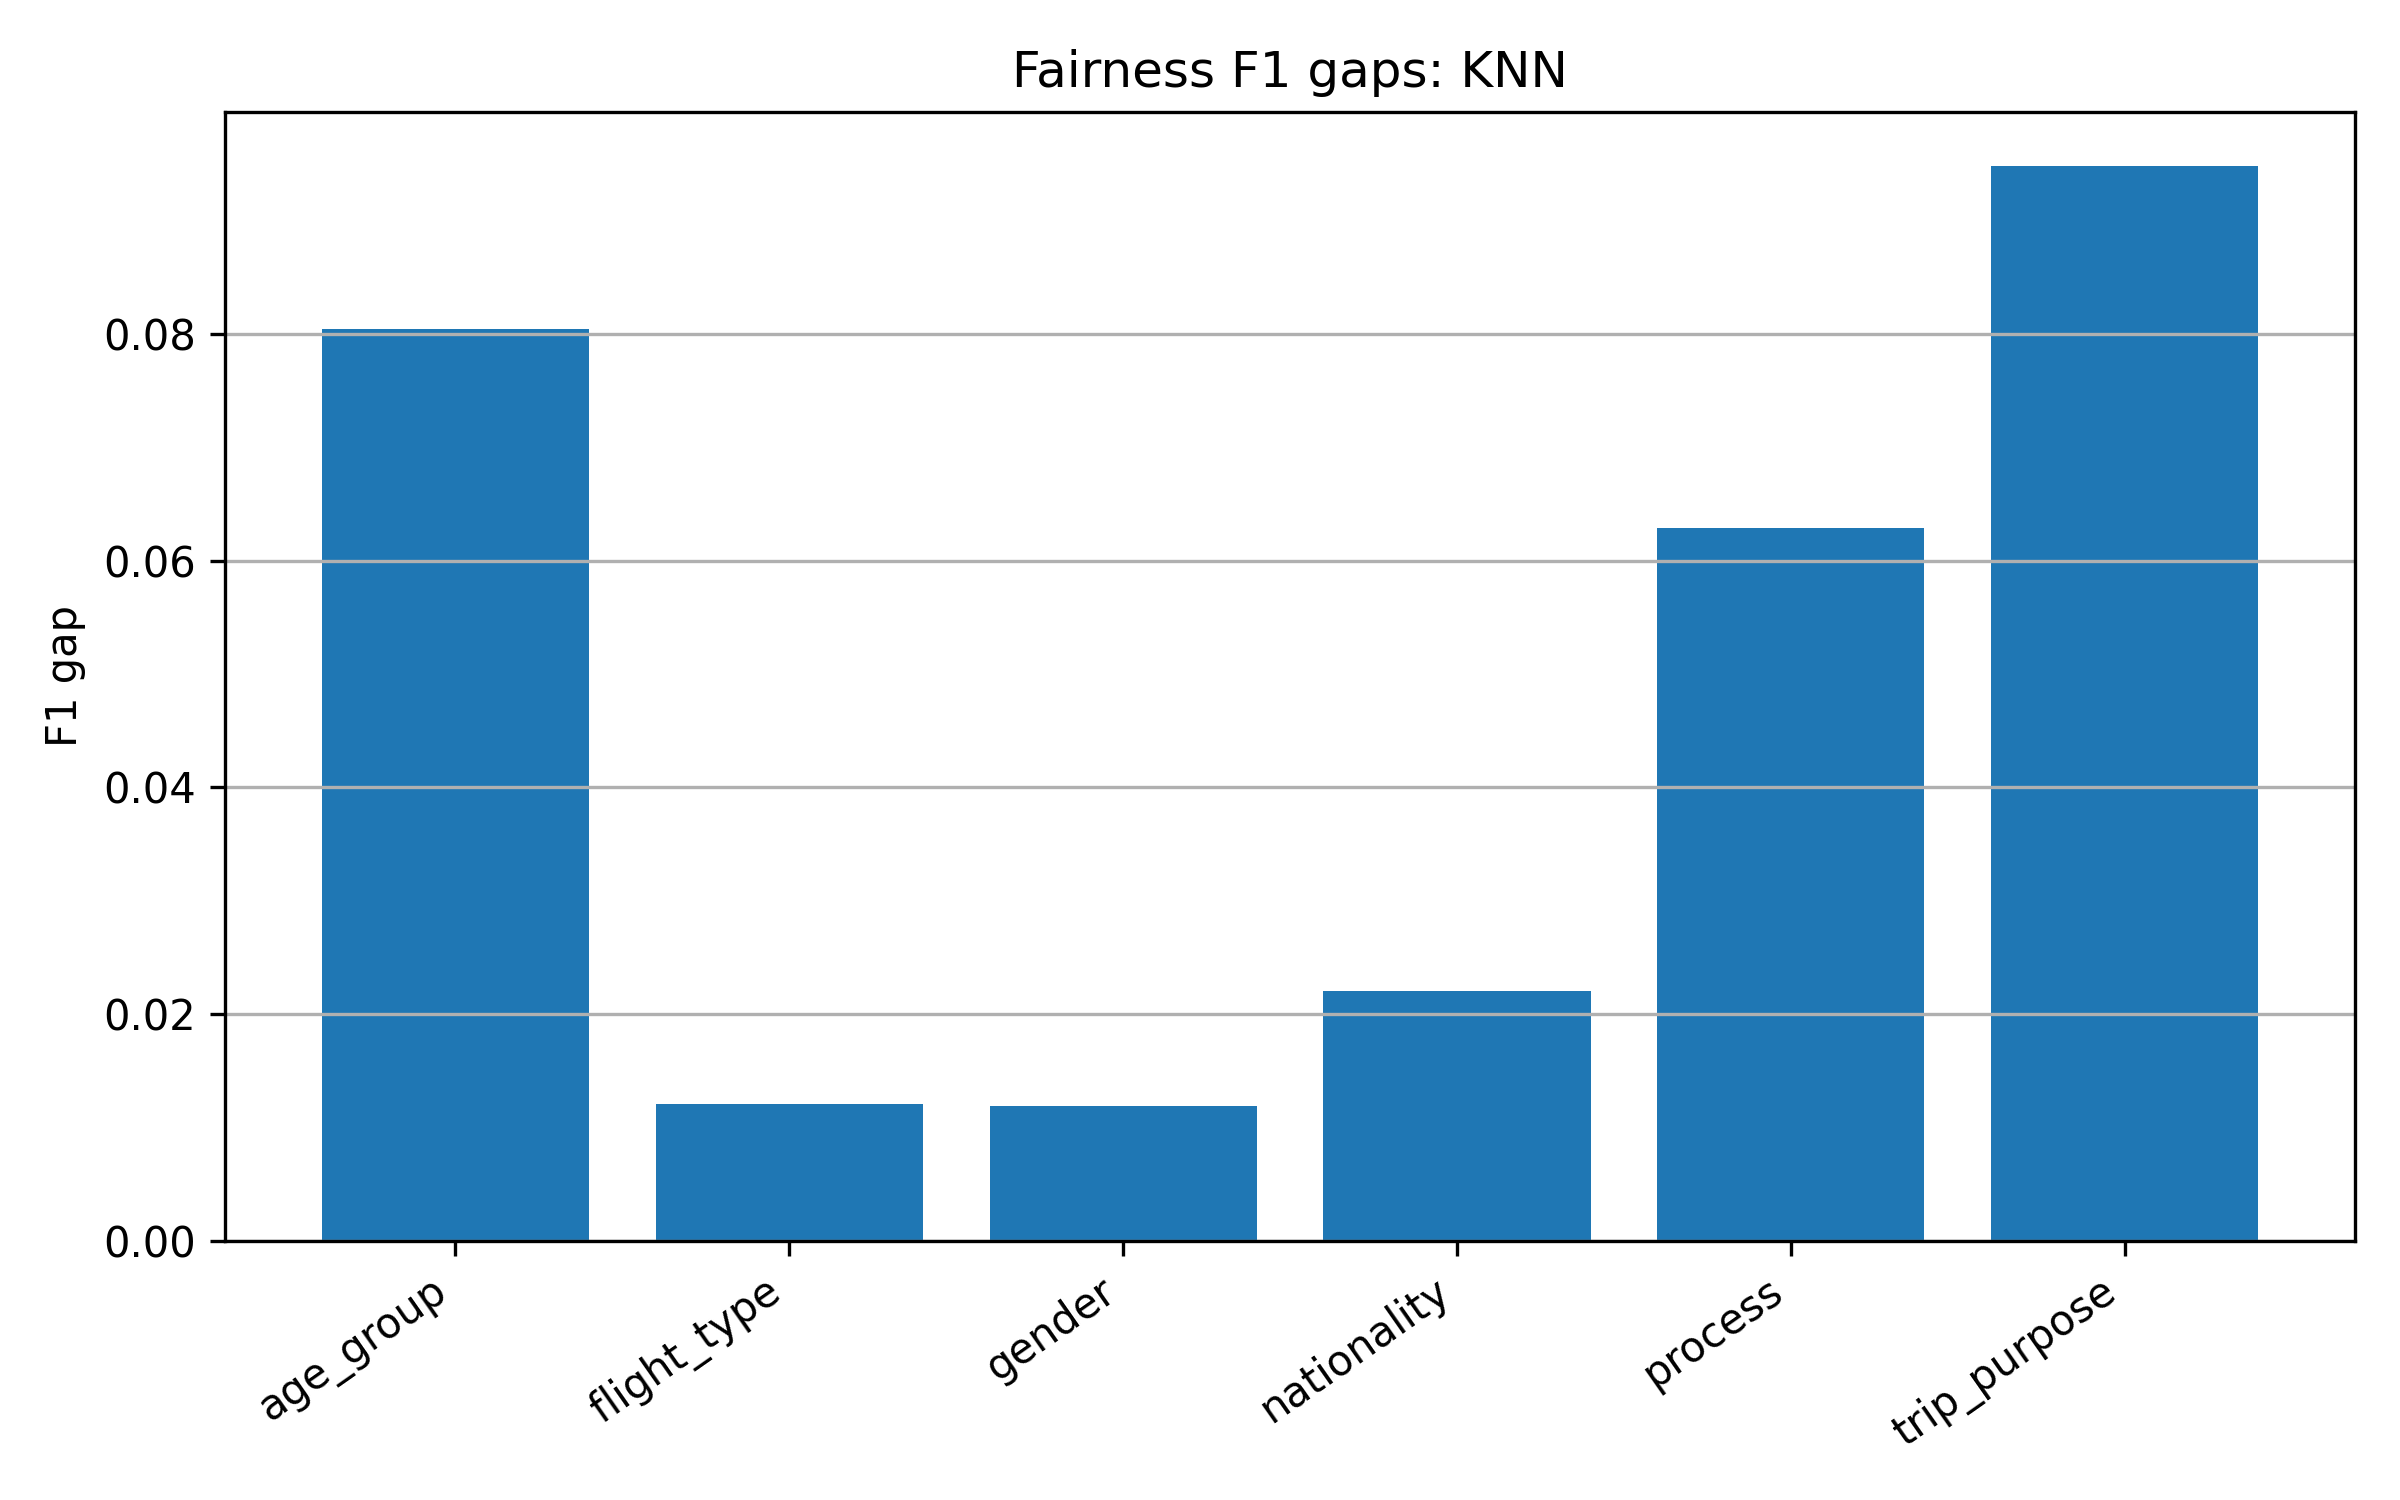
\includegraphics[width=0.82\textwidth]{knn_images/knn_fairness_f1_gaps.png}
\caption{Fairness gaps по F1-macro: KNN}
\end{figure}
\begin{figure}[H]
\centering
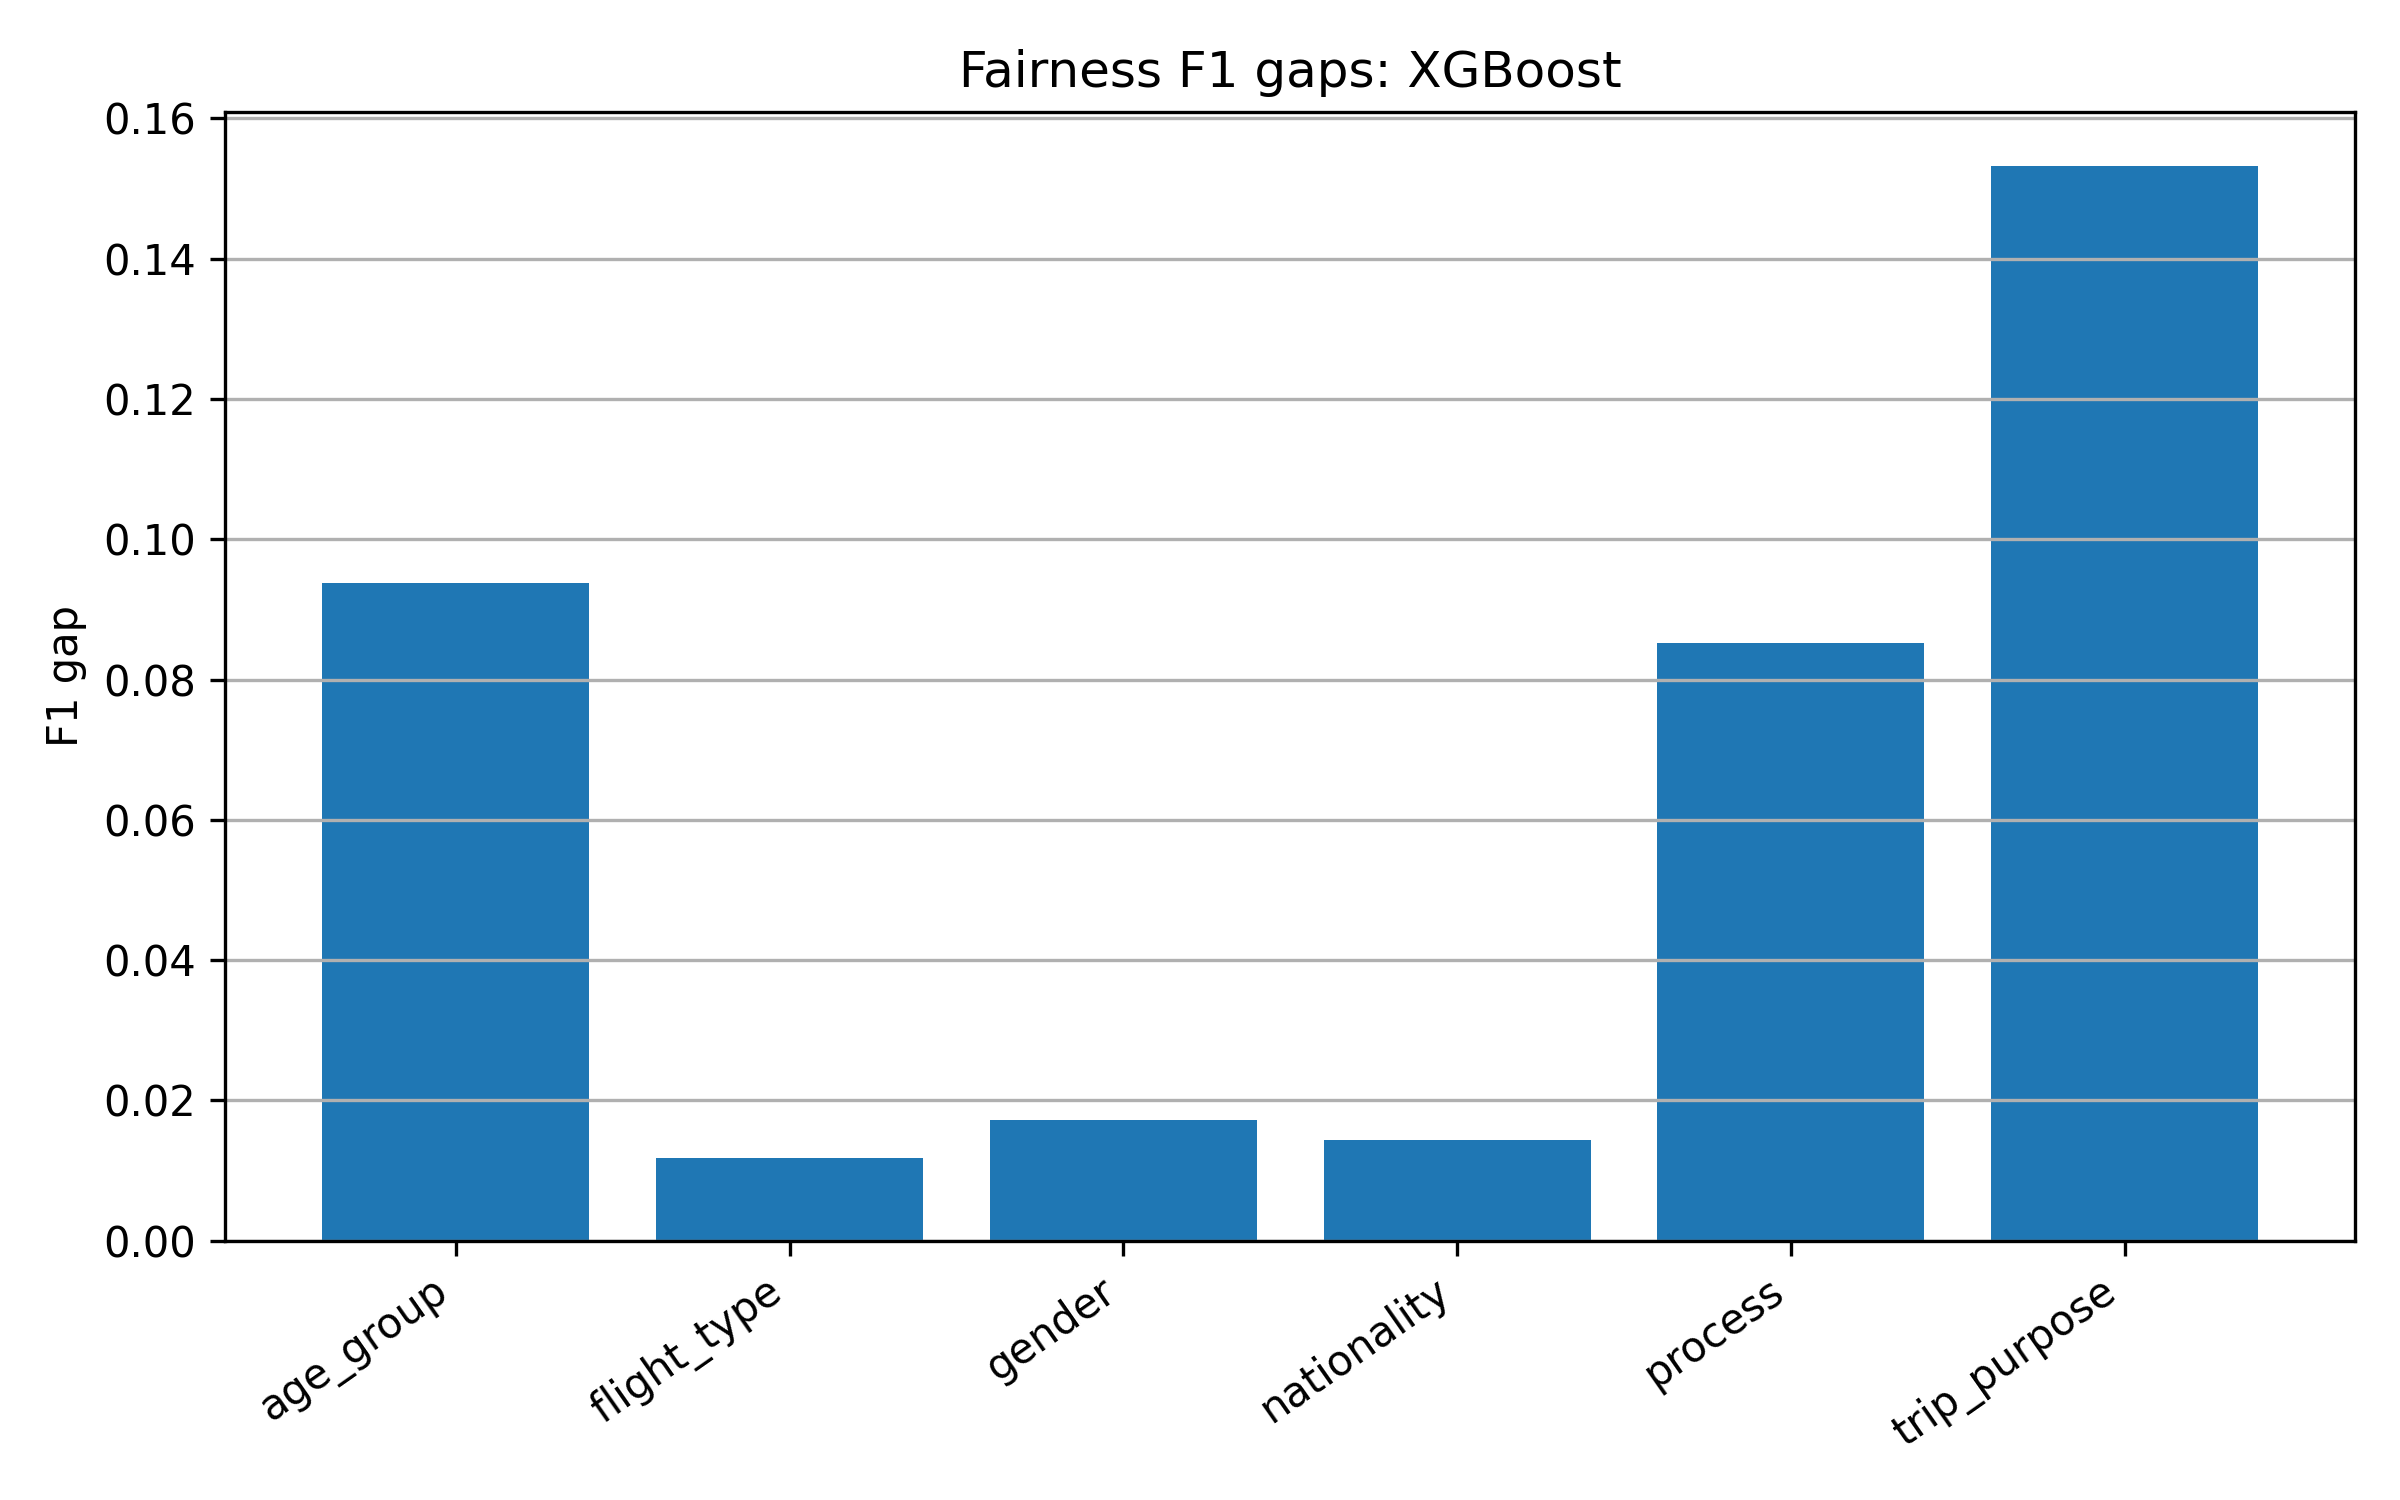
\includegraphics[width=0.82\textwidth]{xgboost_images/xgboost_fairness_f1_gaps.png}
\caption{Fairness gaps по F1-macro: XGBoost}
\end{figure}
\begin{figure}[H]
\centering
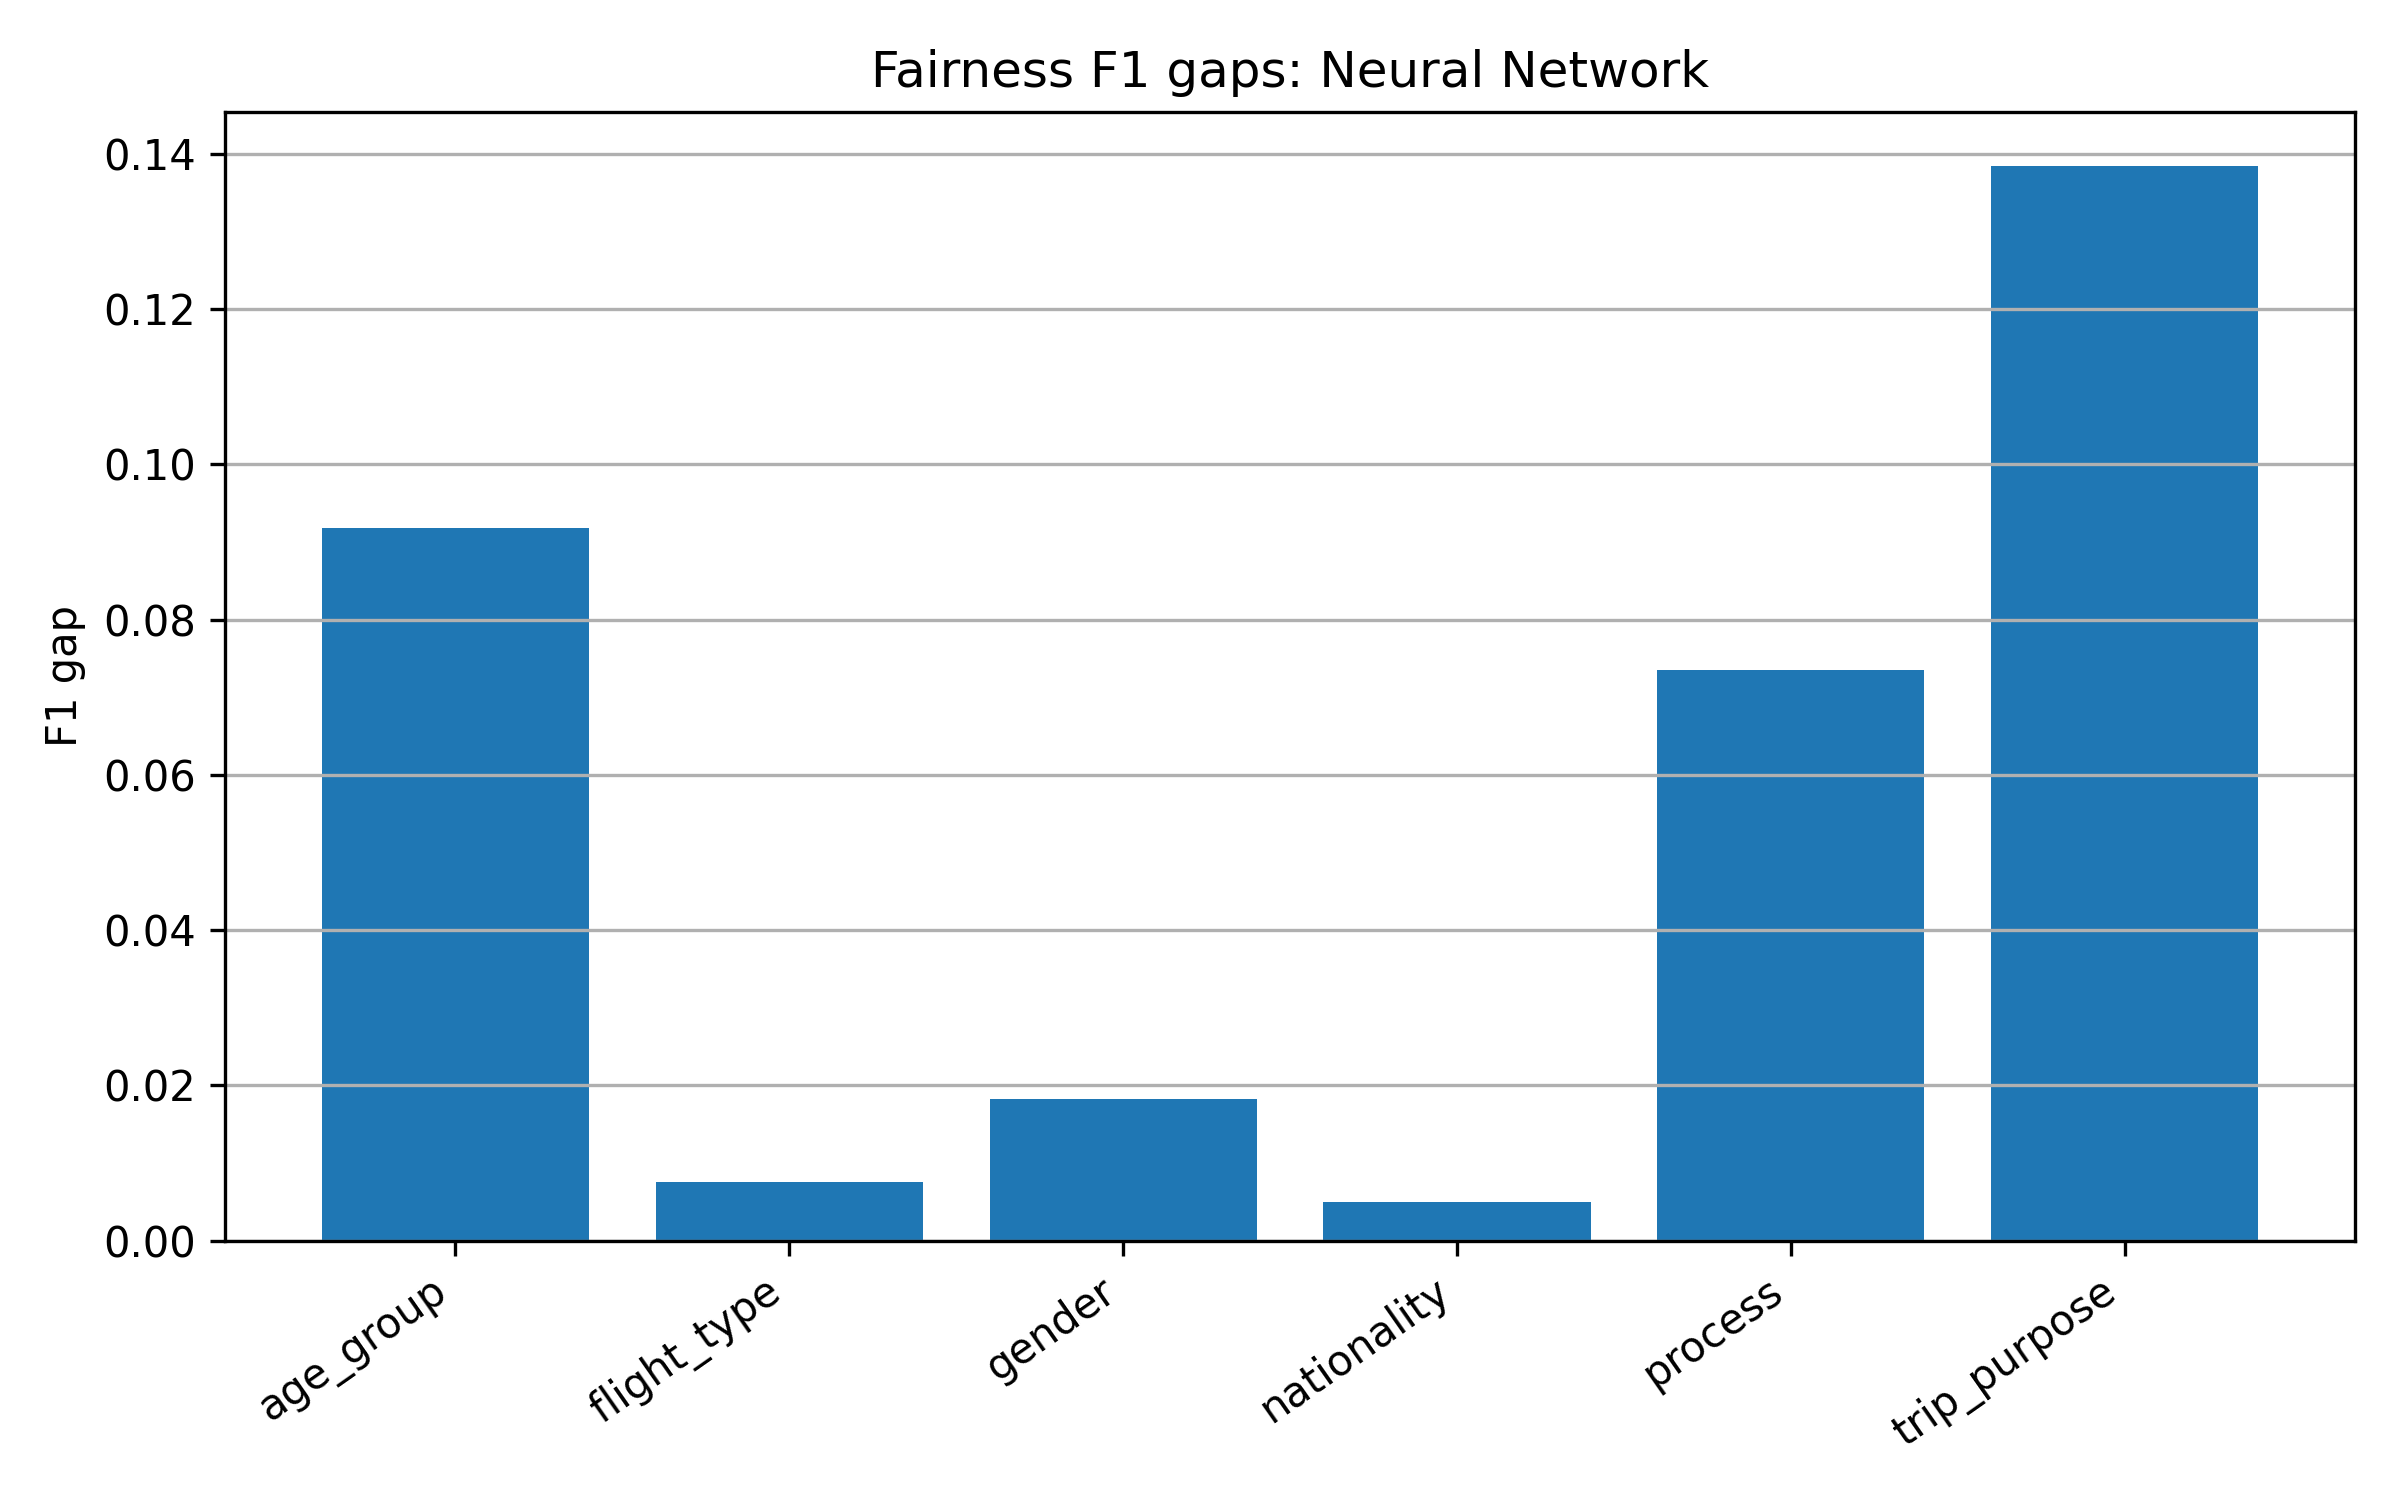
\includegraphics[width=0.82\textwidth]{neural_network_images/neural_network_fairness_f1_gaps.png}
\caption{Fairness gaps по F1-macro: Neural Network}
\end{figure}

Наиболее заметные различия качества наблюдаются по цели поездки, возрастным группам и типу процесса обслуживания. Это может быть связано с тем, что пассажиры разных групп проходят разные этапы аэропортового сервиса и имеют разные ожидания от перелета. Например, бизнес-пассажиры и туристы могут по-разному реагировать на ожидание, навигацию и комфорт терминала. При практическом внедрении модели такие различия требуют дополнительного мониторинга: итоговая модель не должна оцениваться только по среднему F1, поскольку одинаковое среднее качество может скрывать заметные провалы на отдельных группах пассажиров.

\section{Анализ ошибок модели}

\scriptsize
\begin{longtable}{lllll}
\caption{Матрицы ошибок в числовом виде}\label{tab:confusion_matrices}\\
\toprule
Модель & TN & FP & FN & TP \\
\midrule
\endfirsthead
\toprule
Модель & TN & FP & FN & TP \\
\midrule
\endhead
Logistic Regression & 2148 & 728 & 362 & 2514 \\
Decision Tree & 2174 & 702 & 424 & 2452 \\
Random Forest & 2175 & 701 & 391 & 2485 \\
KNN & 2180 & 696 & 451 & 2425 \\
XGBoost & 2213 & 663 & 362 & 2514 \\
Neural Network & 2213 & 663 & 405 & 2471 \\
\bottomrule
\end{longtable}
\normalsize
\begin{figure}[H]
\centering
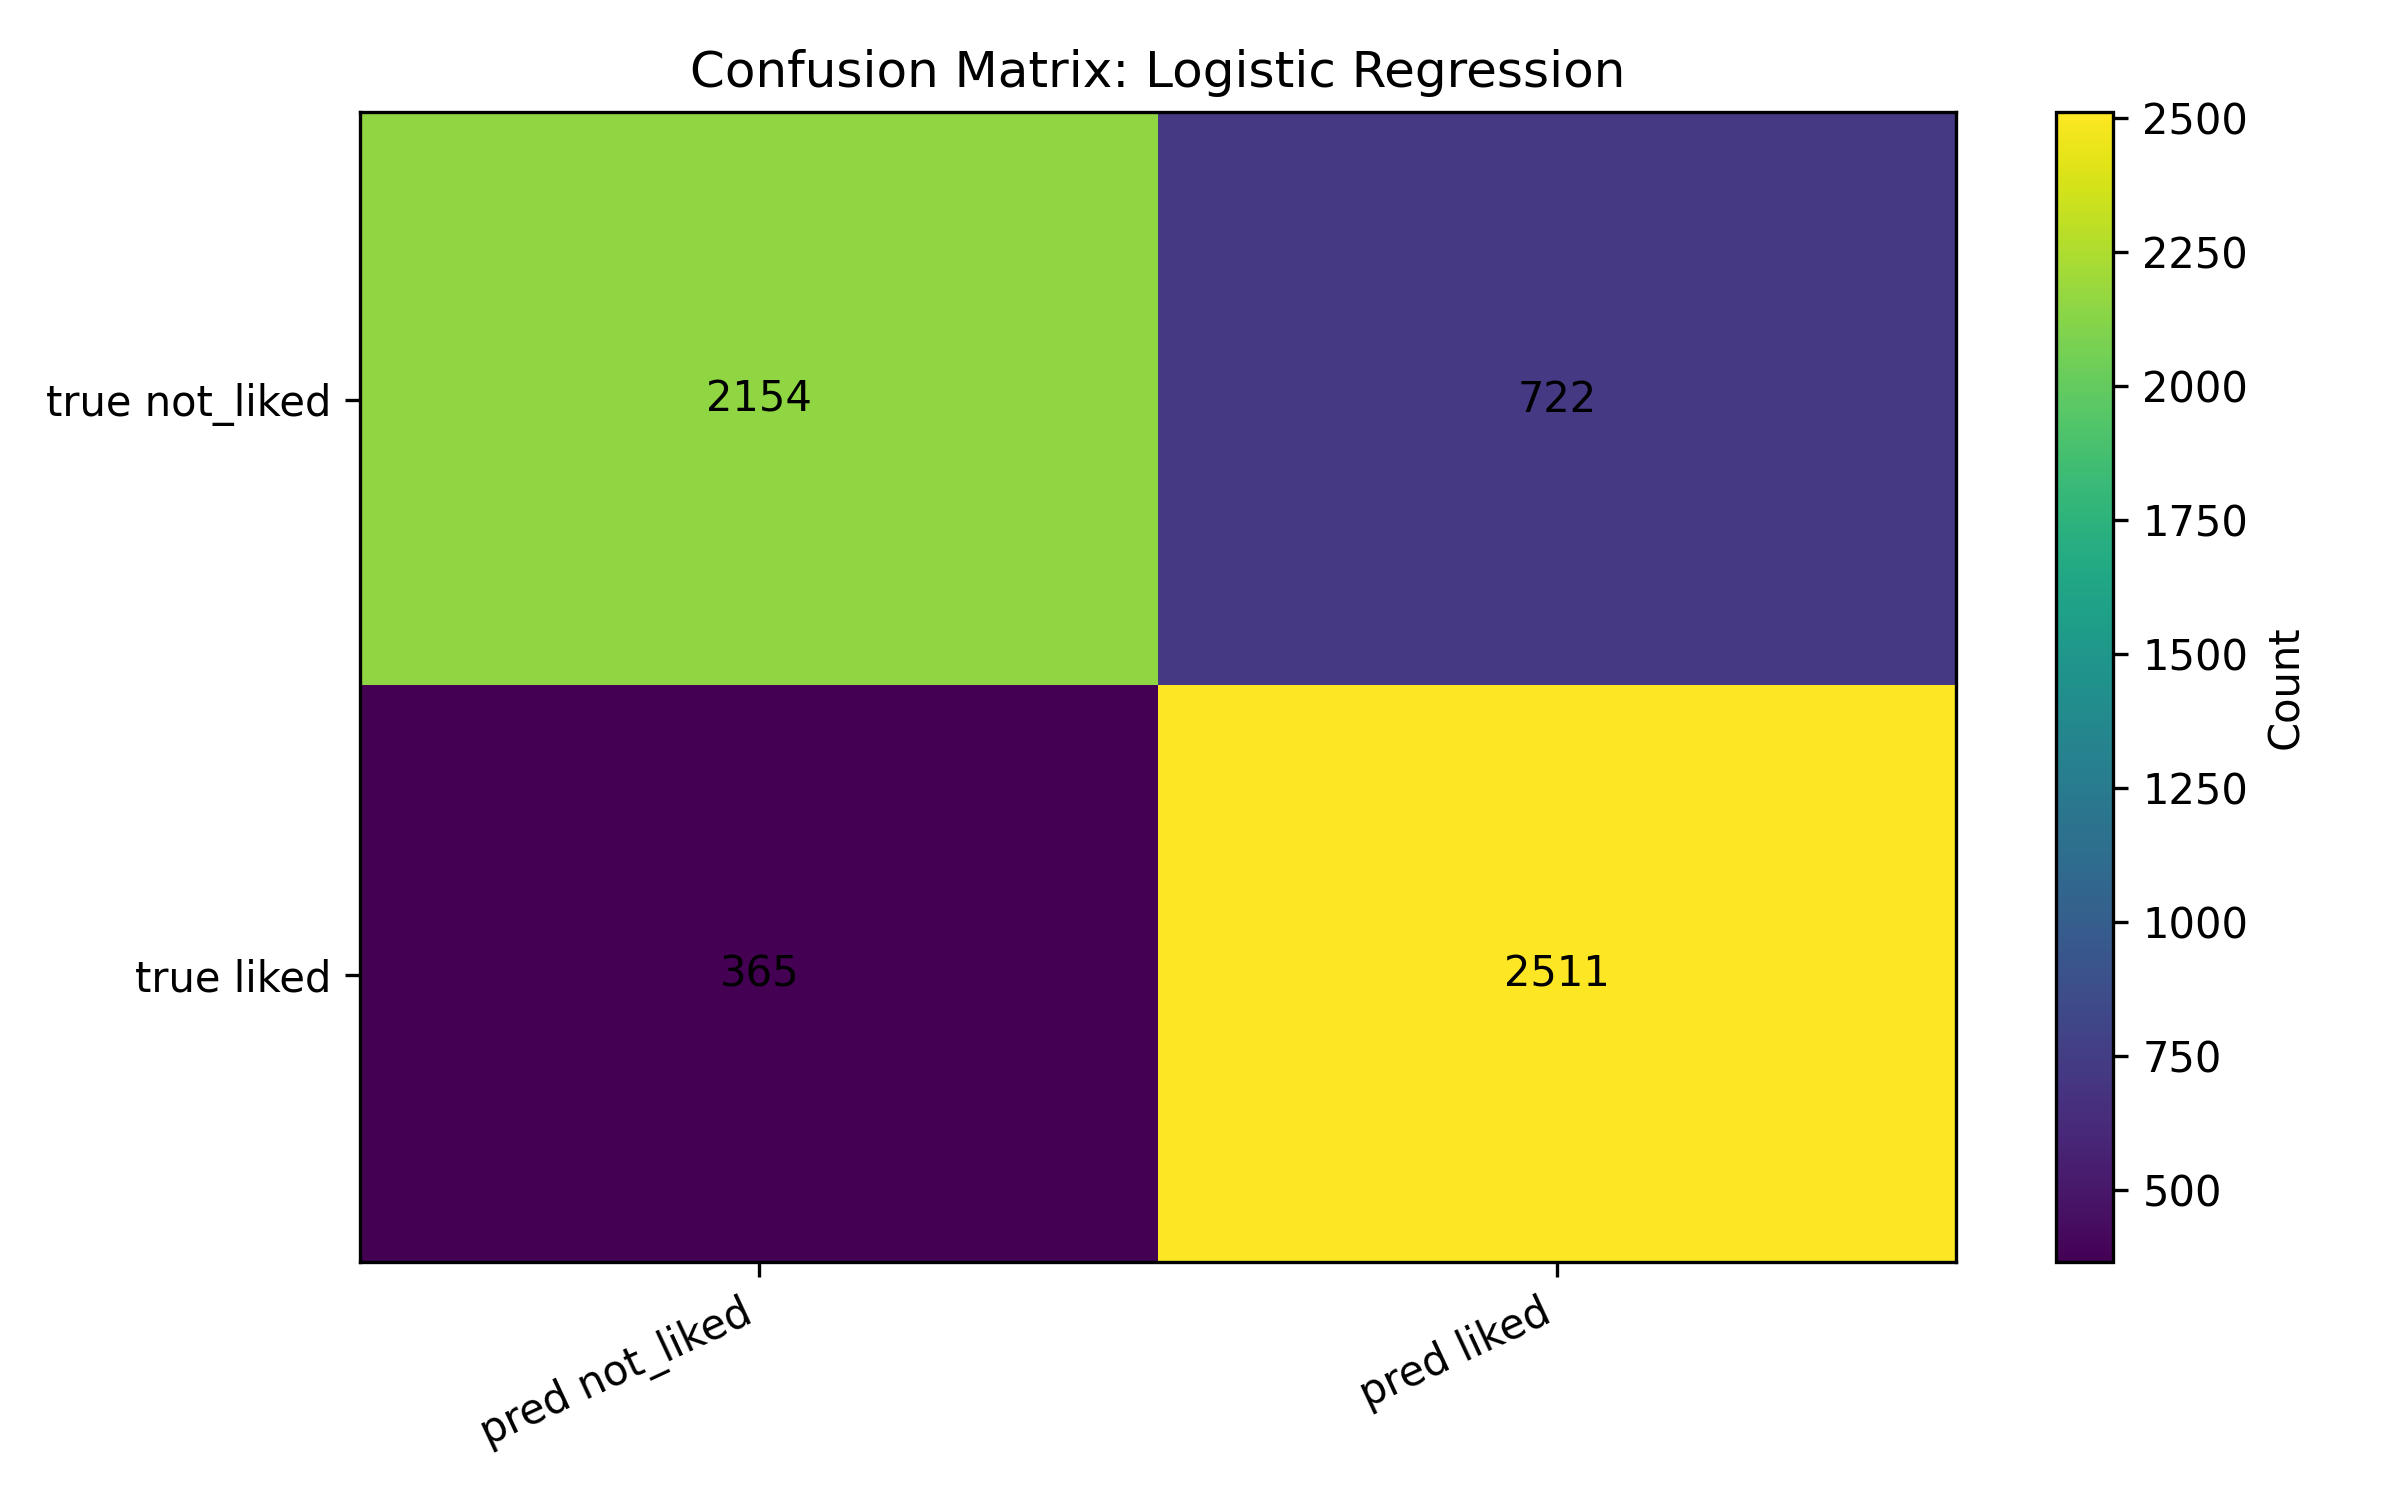
\includegraphics[width=0.82\textwidth]{logistic_regression_images/logistic_regression_confusion_matrix.png}
\caption{Матрица ошибок: Logistic Regression}
\end{figure}
\begin{figure}[H]
\centering
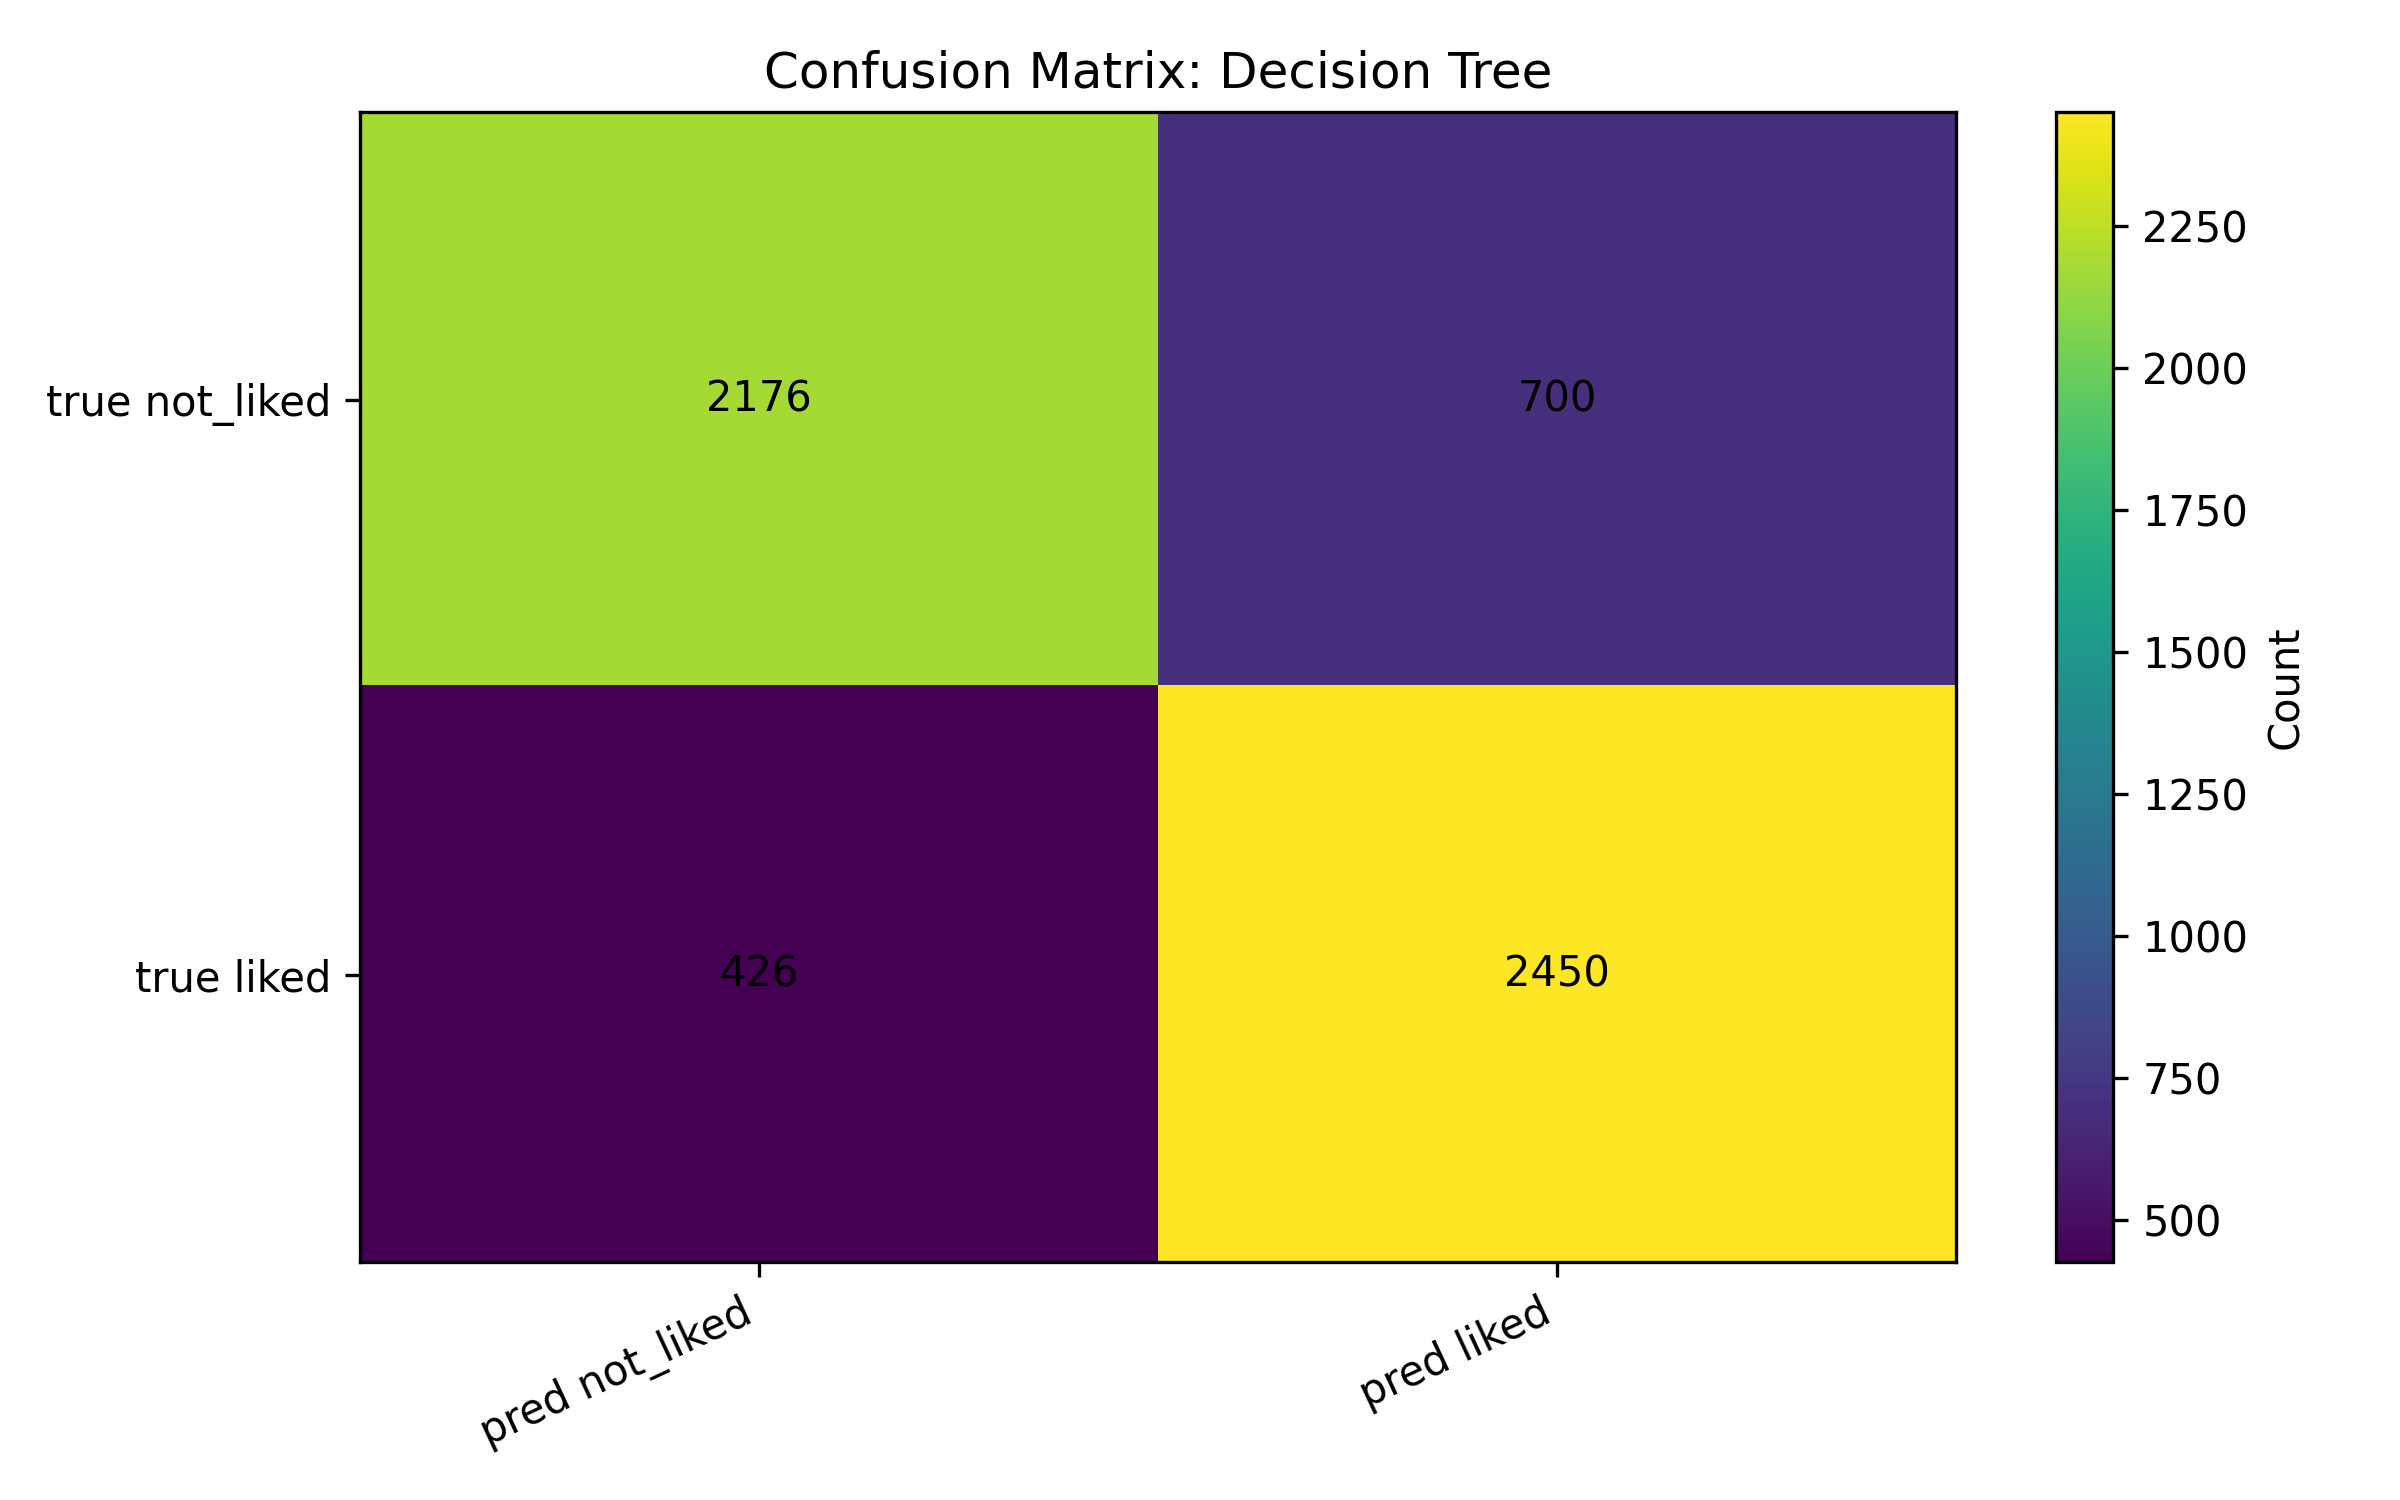
\includegraphics[width=0.82\textwidth]{decision_tree_images/decision_tree_confusion_matrix.png}
\caption{Матрица ошибок: Decision Tree}
\end{figure}
\begin{figure}[H]
\centering
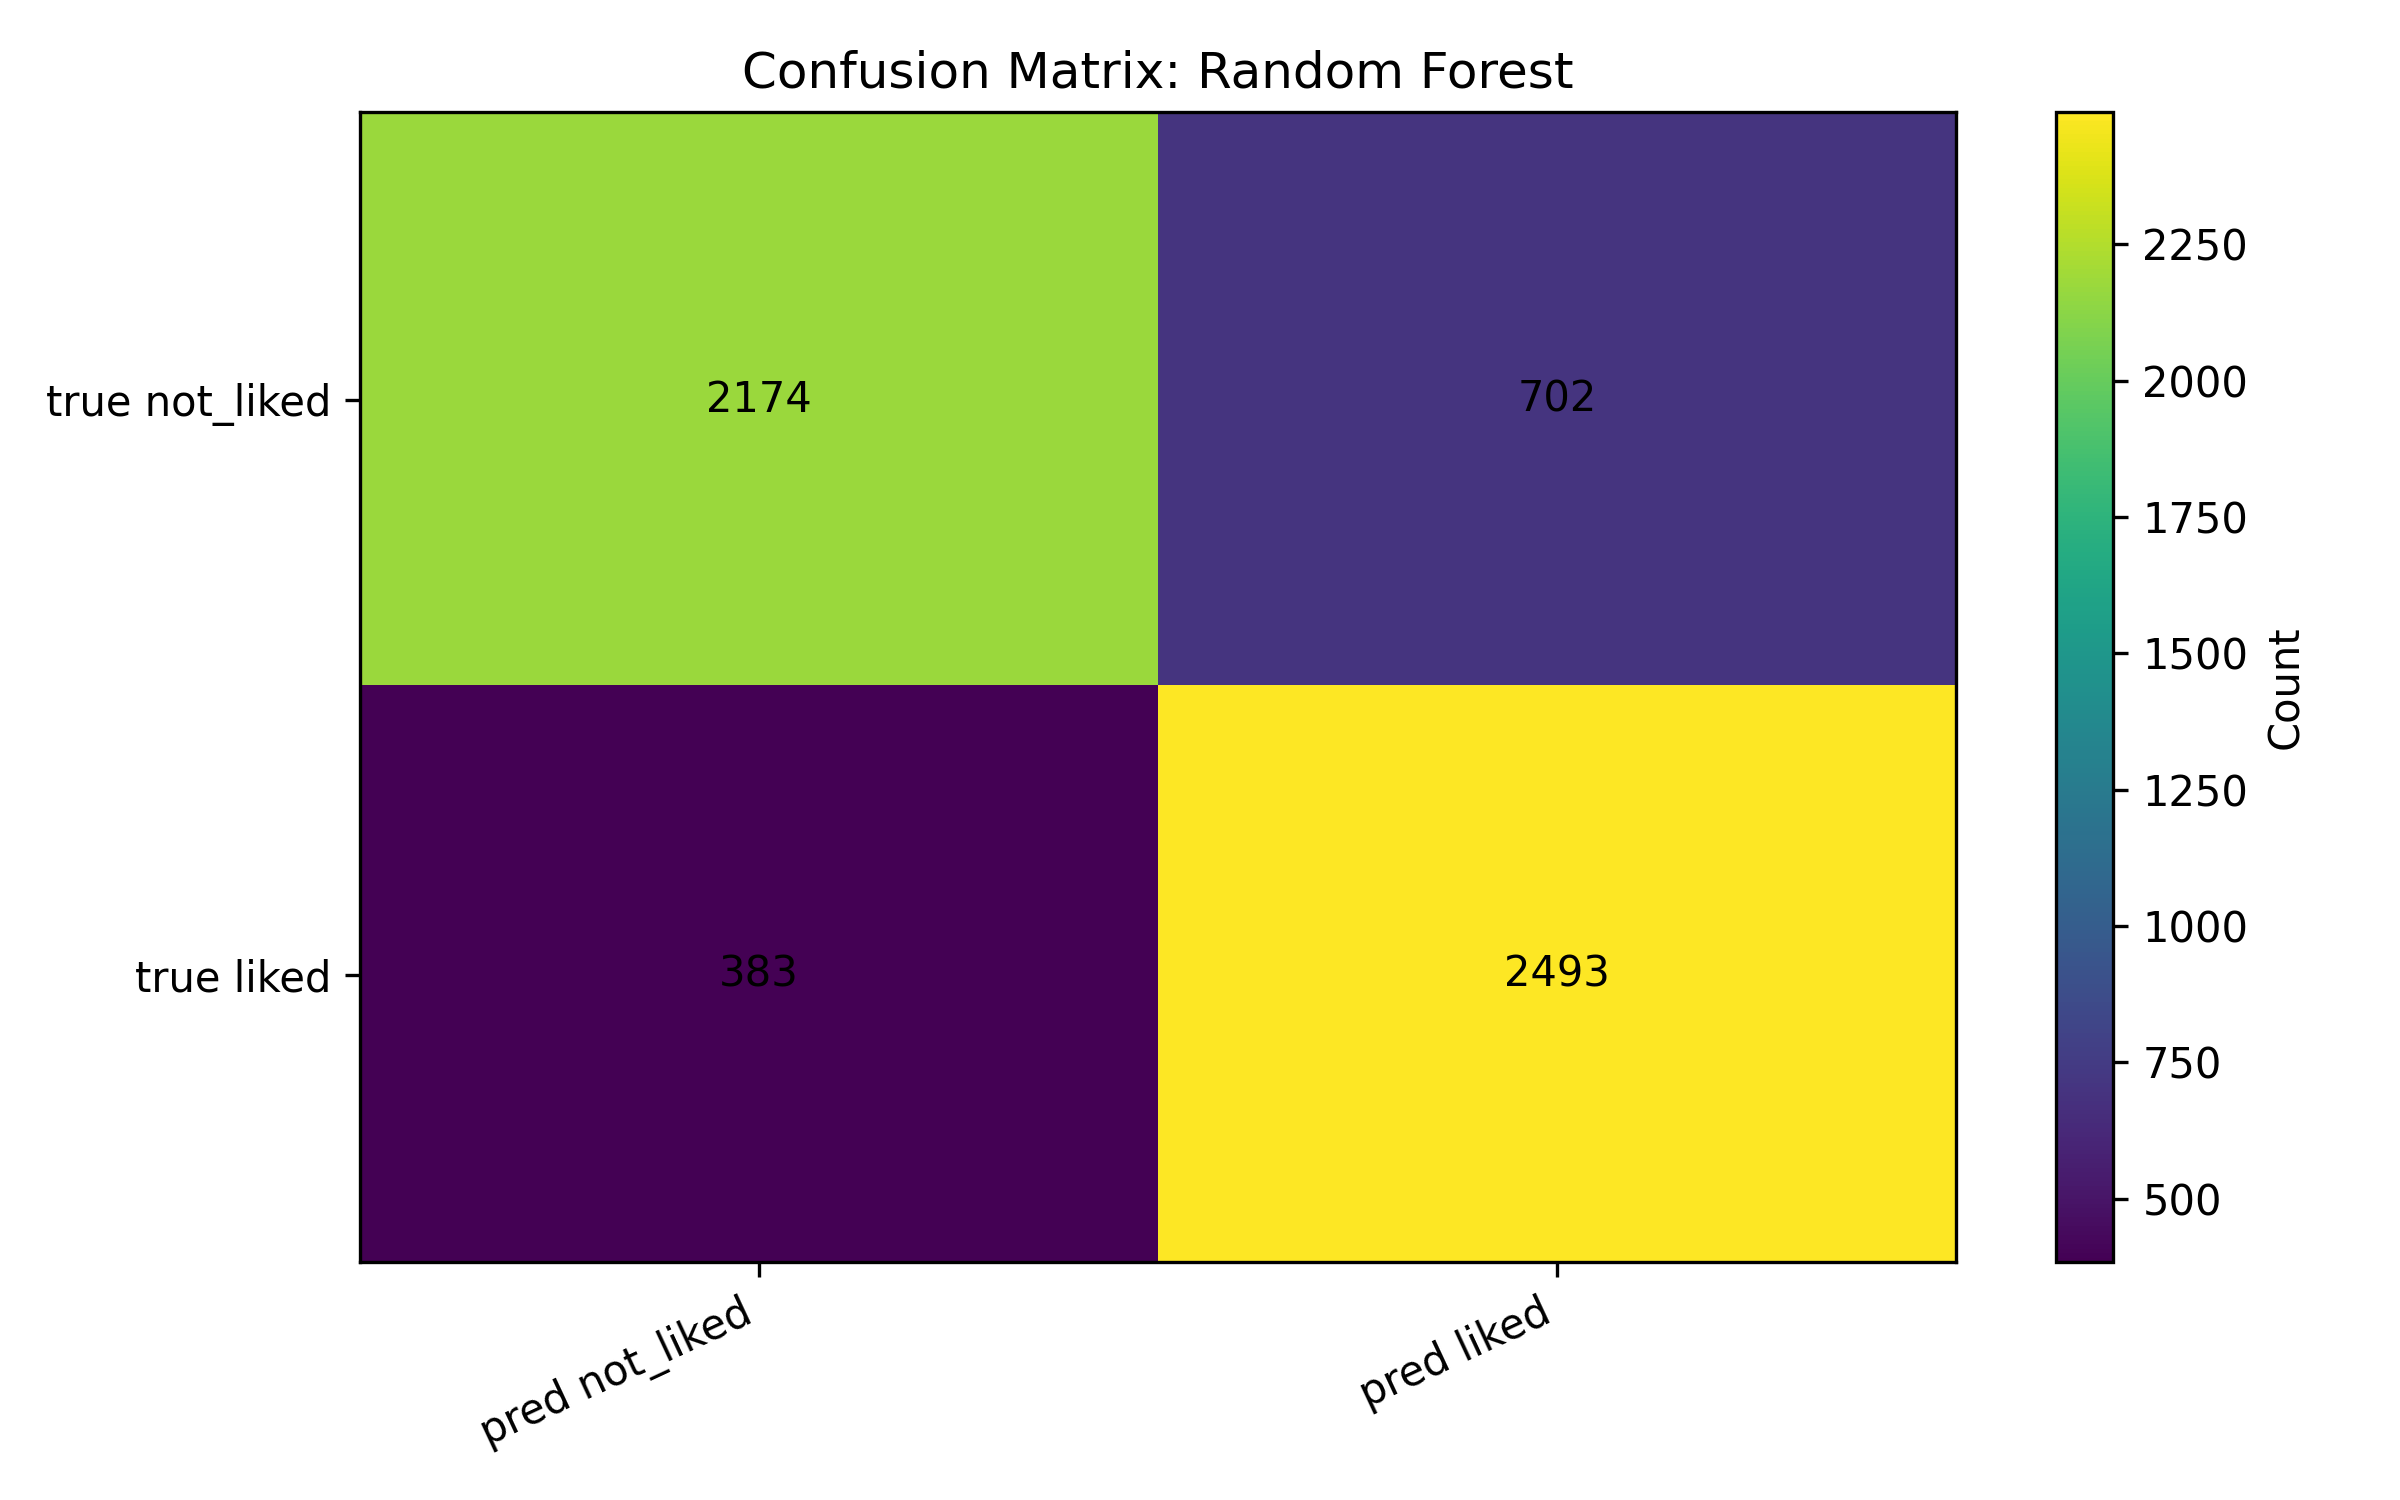
\includegraphics[width=0.82\textwidth]{random_forest_images/random_forest_confusion_matrix.png}
\caption{Матрица ошибок: Random Forest}
\end{figure}
\begin{figure}[H]
\centering
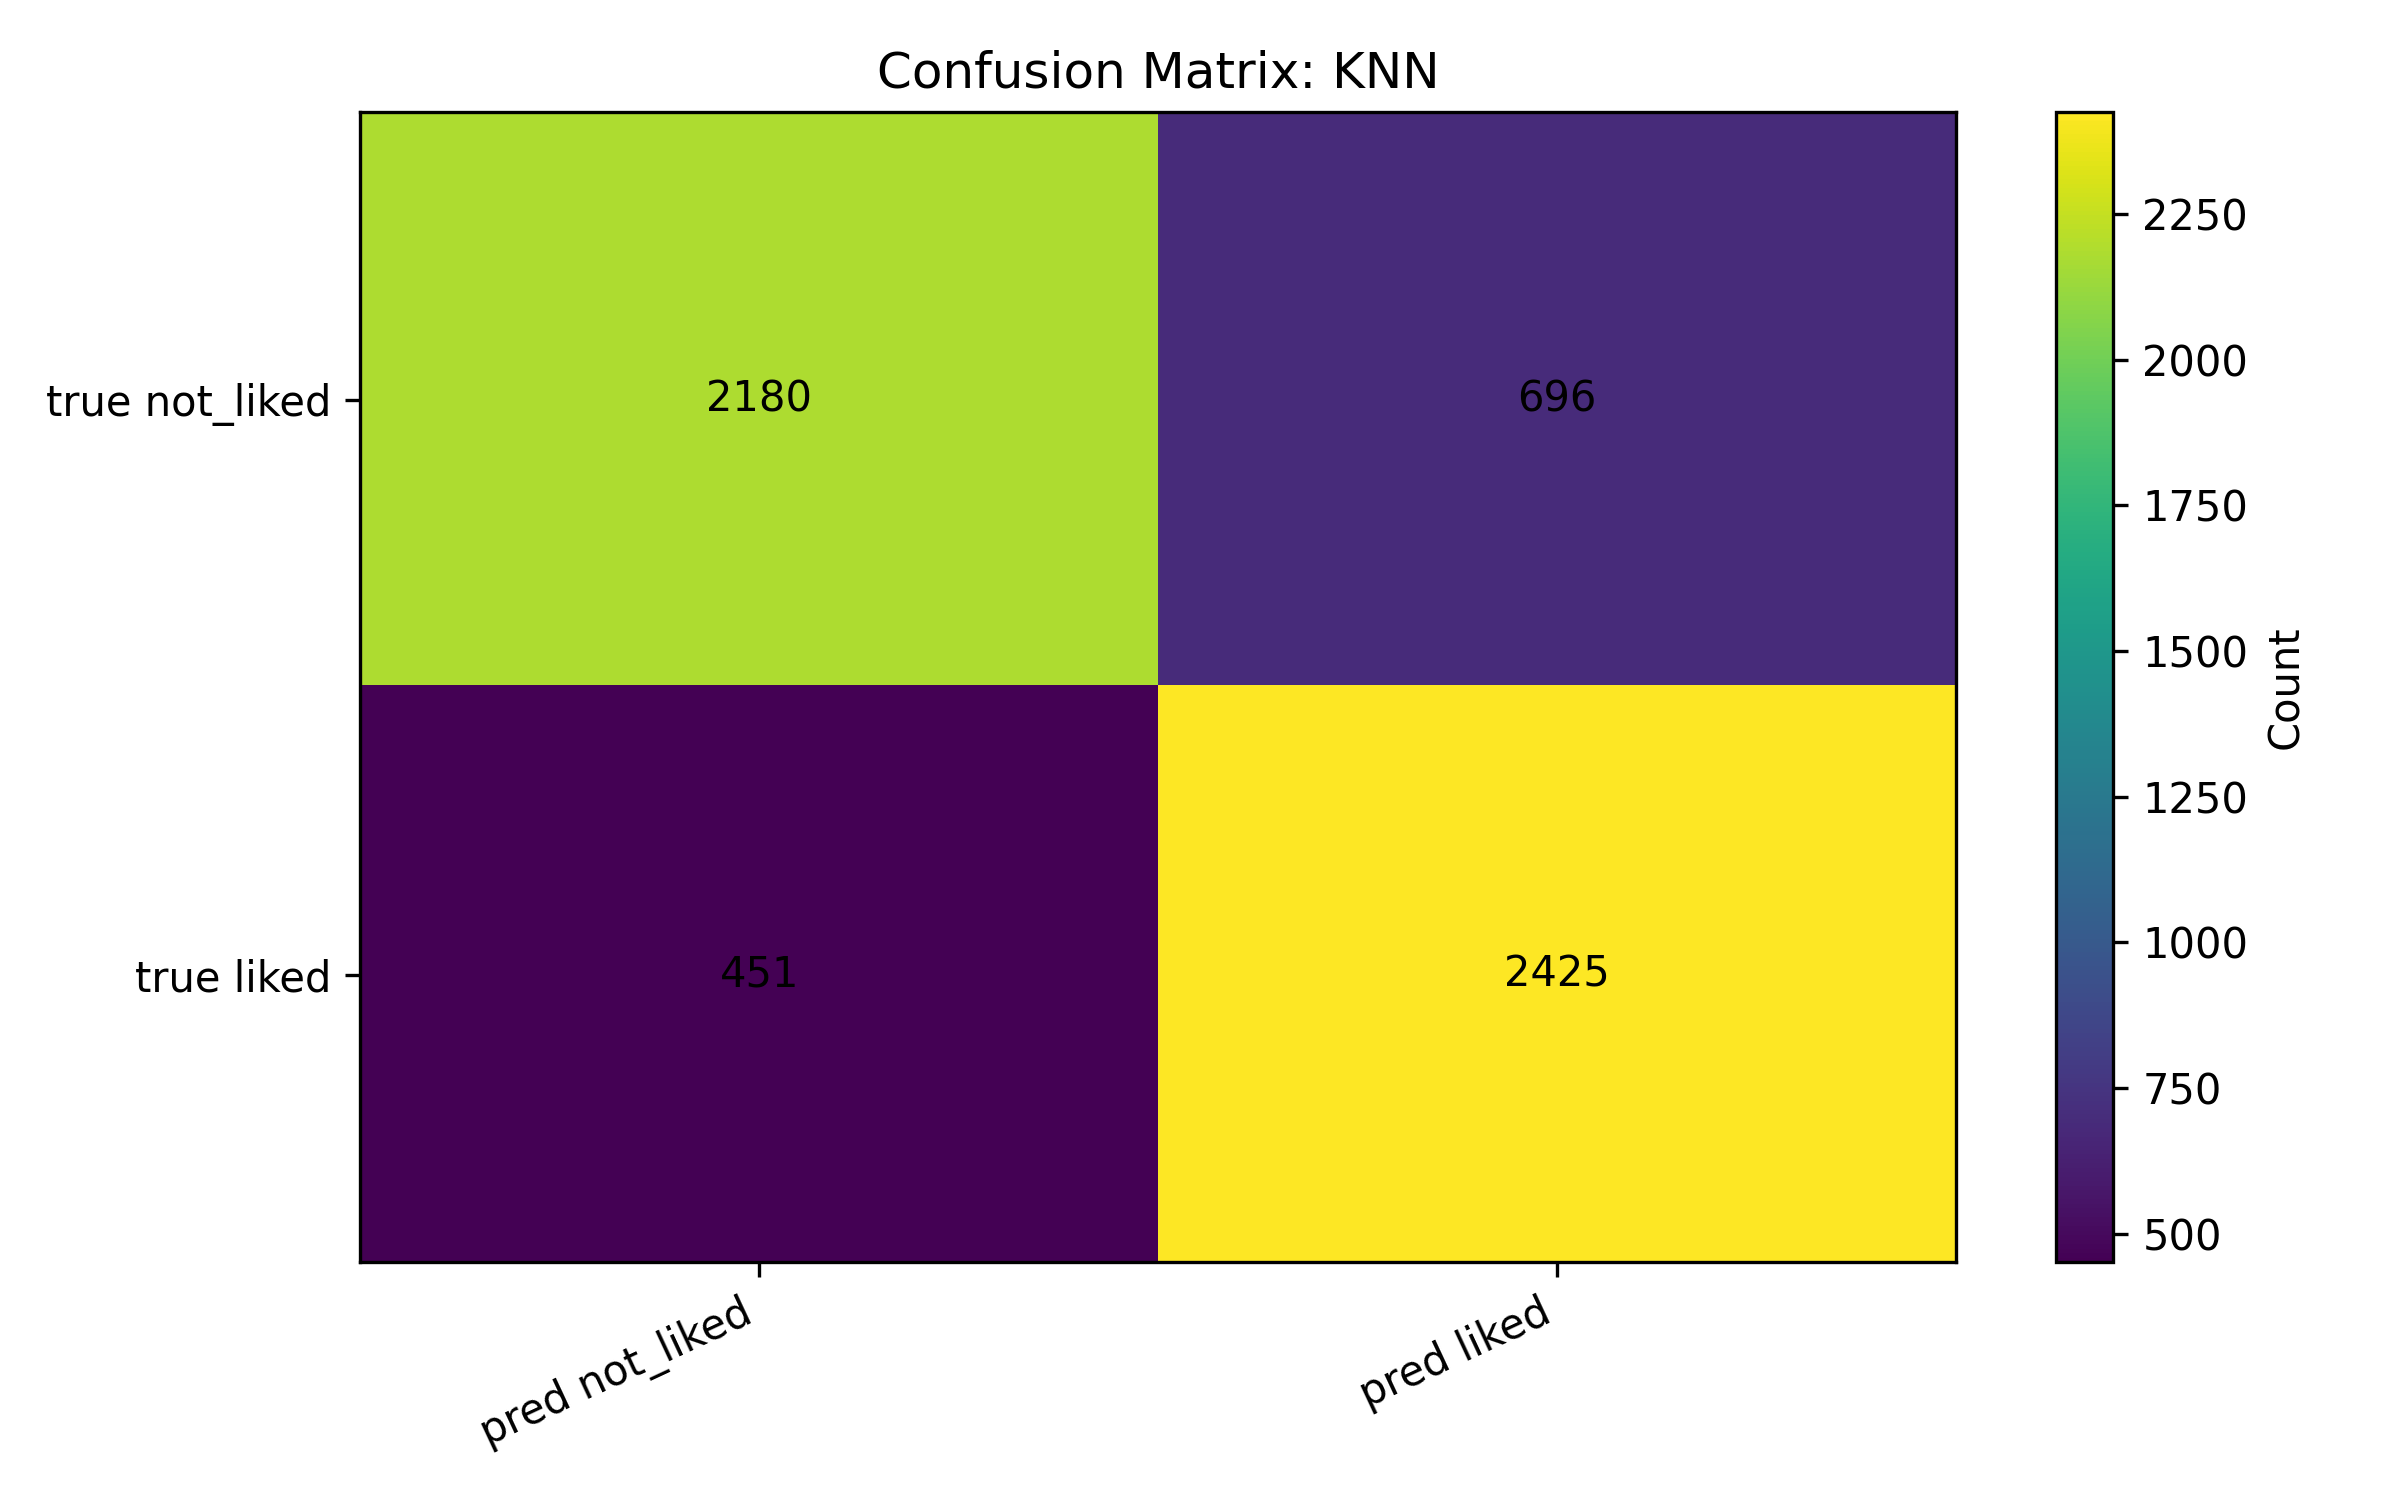
\includegraphics[width=0.82\textwidth]{knn_images/knn_confusion_matrix.png}
\caption{Матрица ошибок: KNN}
\end{figure}
\begin{figure}[H]
\centering
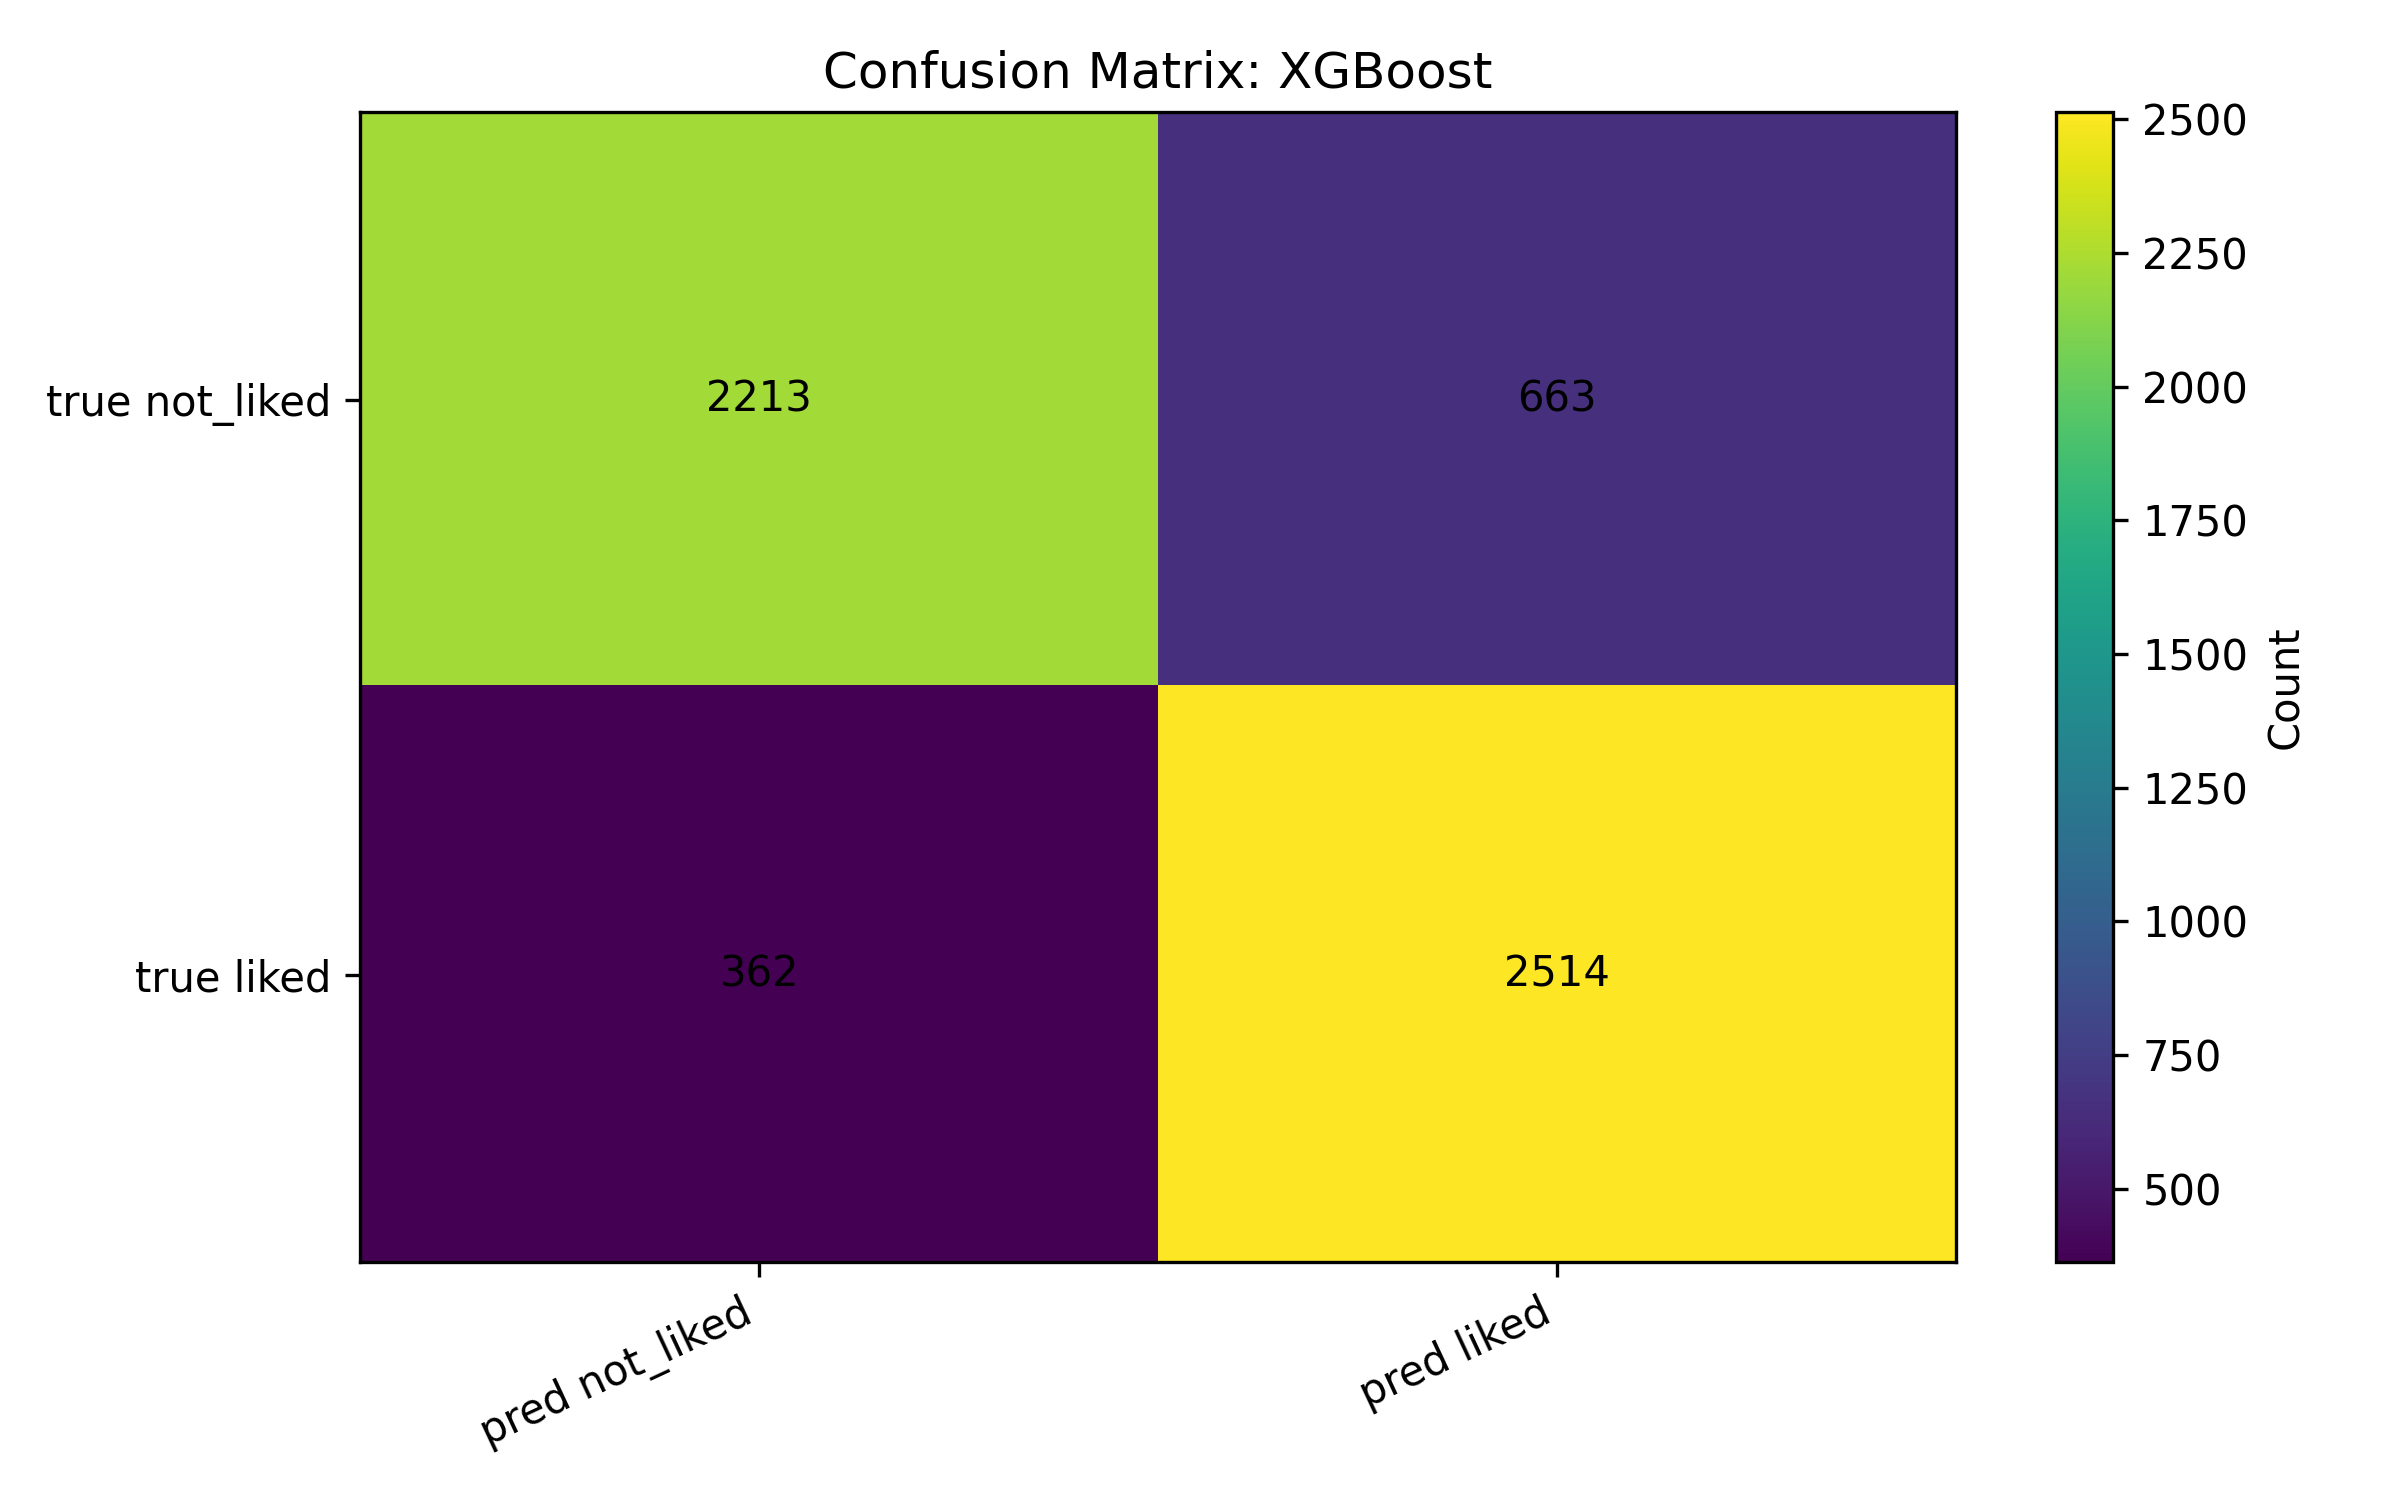
\includegraphics[width=0.82\textwidth]{xgboost_images/xgboost_confusion_matrix.png}
\caption{Матрица ошибок: XGBoost}
\end{figure}
\begin{figure}[H]
\centering
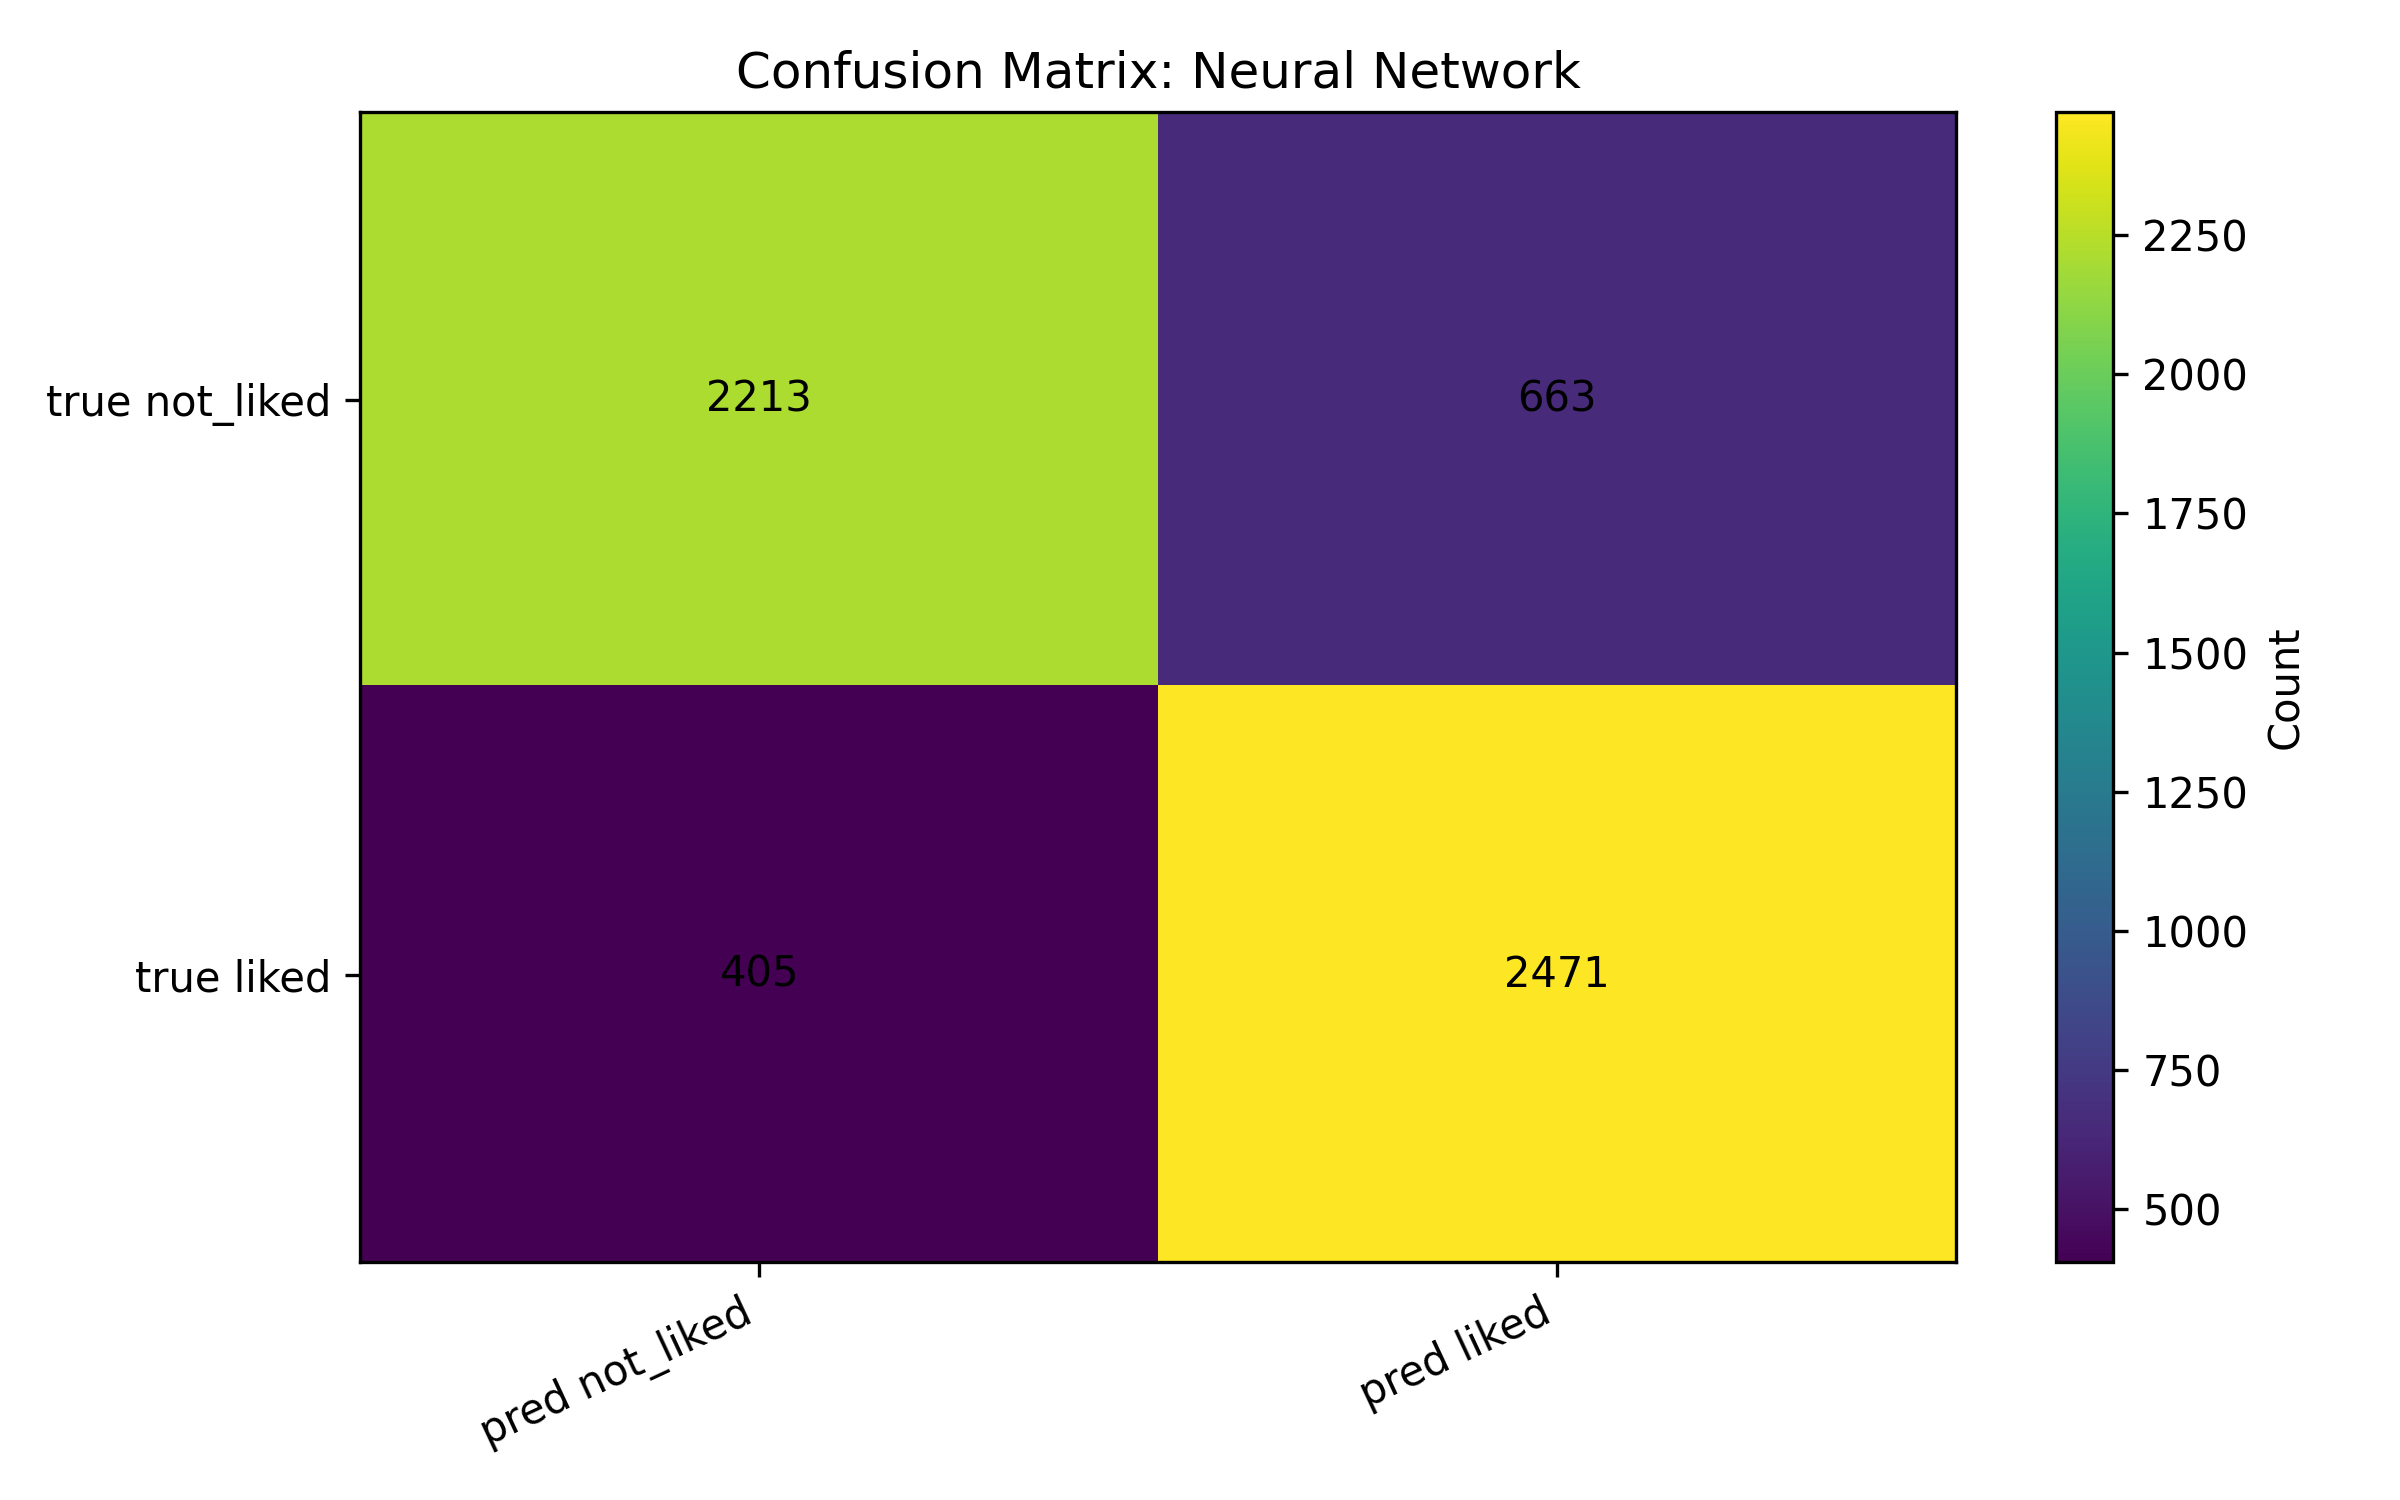
\includegraphics[width=0.82\textwidth]{neural_network_images/neural_network_confusion_matrix.png}
\caption{Матрица ошибок: Neural Network}
\end{figure}

Матрица ошибок показывает баланс между false positive и false negative. В данной задаче оба типа ошибок важны: false negative означает, что неудовлетворенный пассажир не был выявлен, а false positive означает, что ресурсы улучшения сервиса могут быть направлены на пассажира, который фактически удовлетворен. XGBoost имеет наименьшее суммарное число ошибок среди рассмотренных моделей, что согласуется с его лучшим F1-macro. Logistic Regression и Random Forest дают близкое число ошибок, но распределяют их немного по-разному. KNN чаще ошибается на положительном классе, что может быть следствием сложности выбора устойчивых соседей в пространстве смешанных признаков.

\section{Анализ порога классификации}

\scriptsize
\begin{longtable}{lllllll}
\caption{Лучшие пороги классификации по F1-macro}\label{tab:thresholds}\\
\toprule
Модель & Порог & F1-macro & Accuracy & Sensitivity & Specificity & Pred. positive rate \\
\midrule
\endfirsthead
\toprule
Модель & Порог & F1-macro & Accuracy & Sensitivity & Specificity & Pred. positive rate \\
\midrule
\endhead
Logistic Regression & 0.55 & 0.813 & 0.813 & 0.845 & 0.781 & 0.532 \\
Decision Tree & 0.50 & 0.804 & 0.804 & 0.853 & 0.756 & 0.548 \\
Random Forest & 0.50 & 0.810 & 0.810 & 0.864 & 0.756 & 0.554 \\
KNN & 0.55 & 0.801 & 0.801 & 0.816 & 0.787 & 0.515 \\
XGBoost & 0.50 & 0.821 & 0.822 & 0.874 & 0.769 & 0.552 \\
Neural Network & 0.50 & 0.814 & 0.814 & 0.859 & 0.769 & 0.545 \\
\bottomrule
\end{longtable}
\normalsize
\begin{figure}[H]
\centering
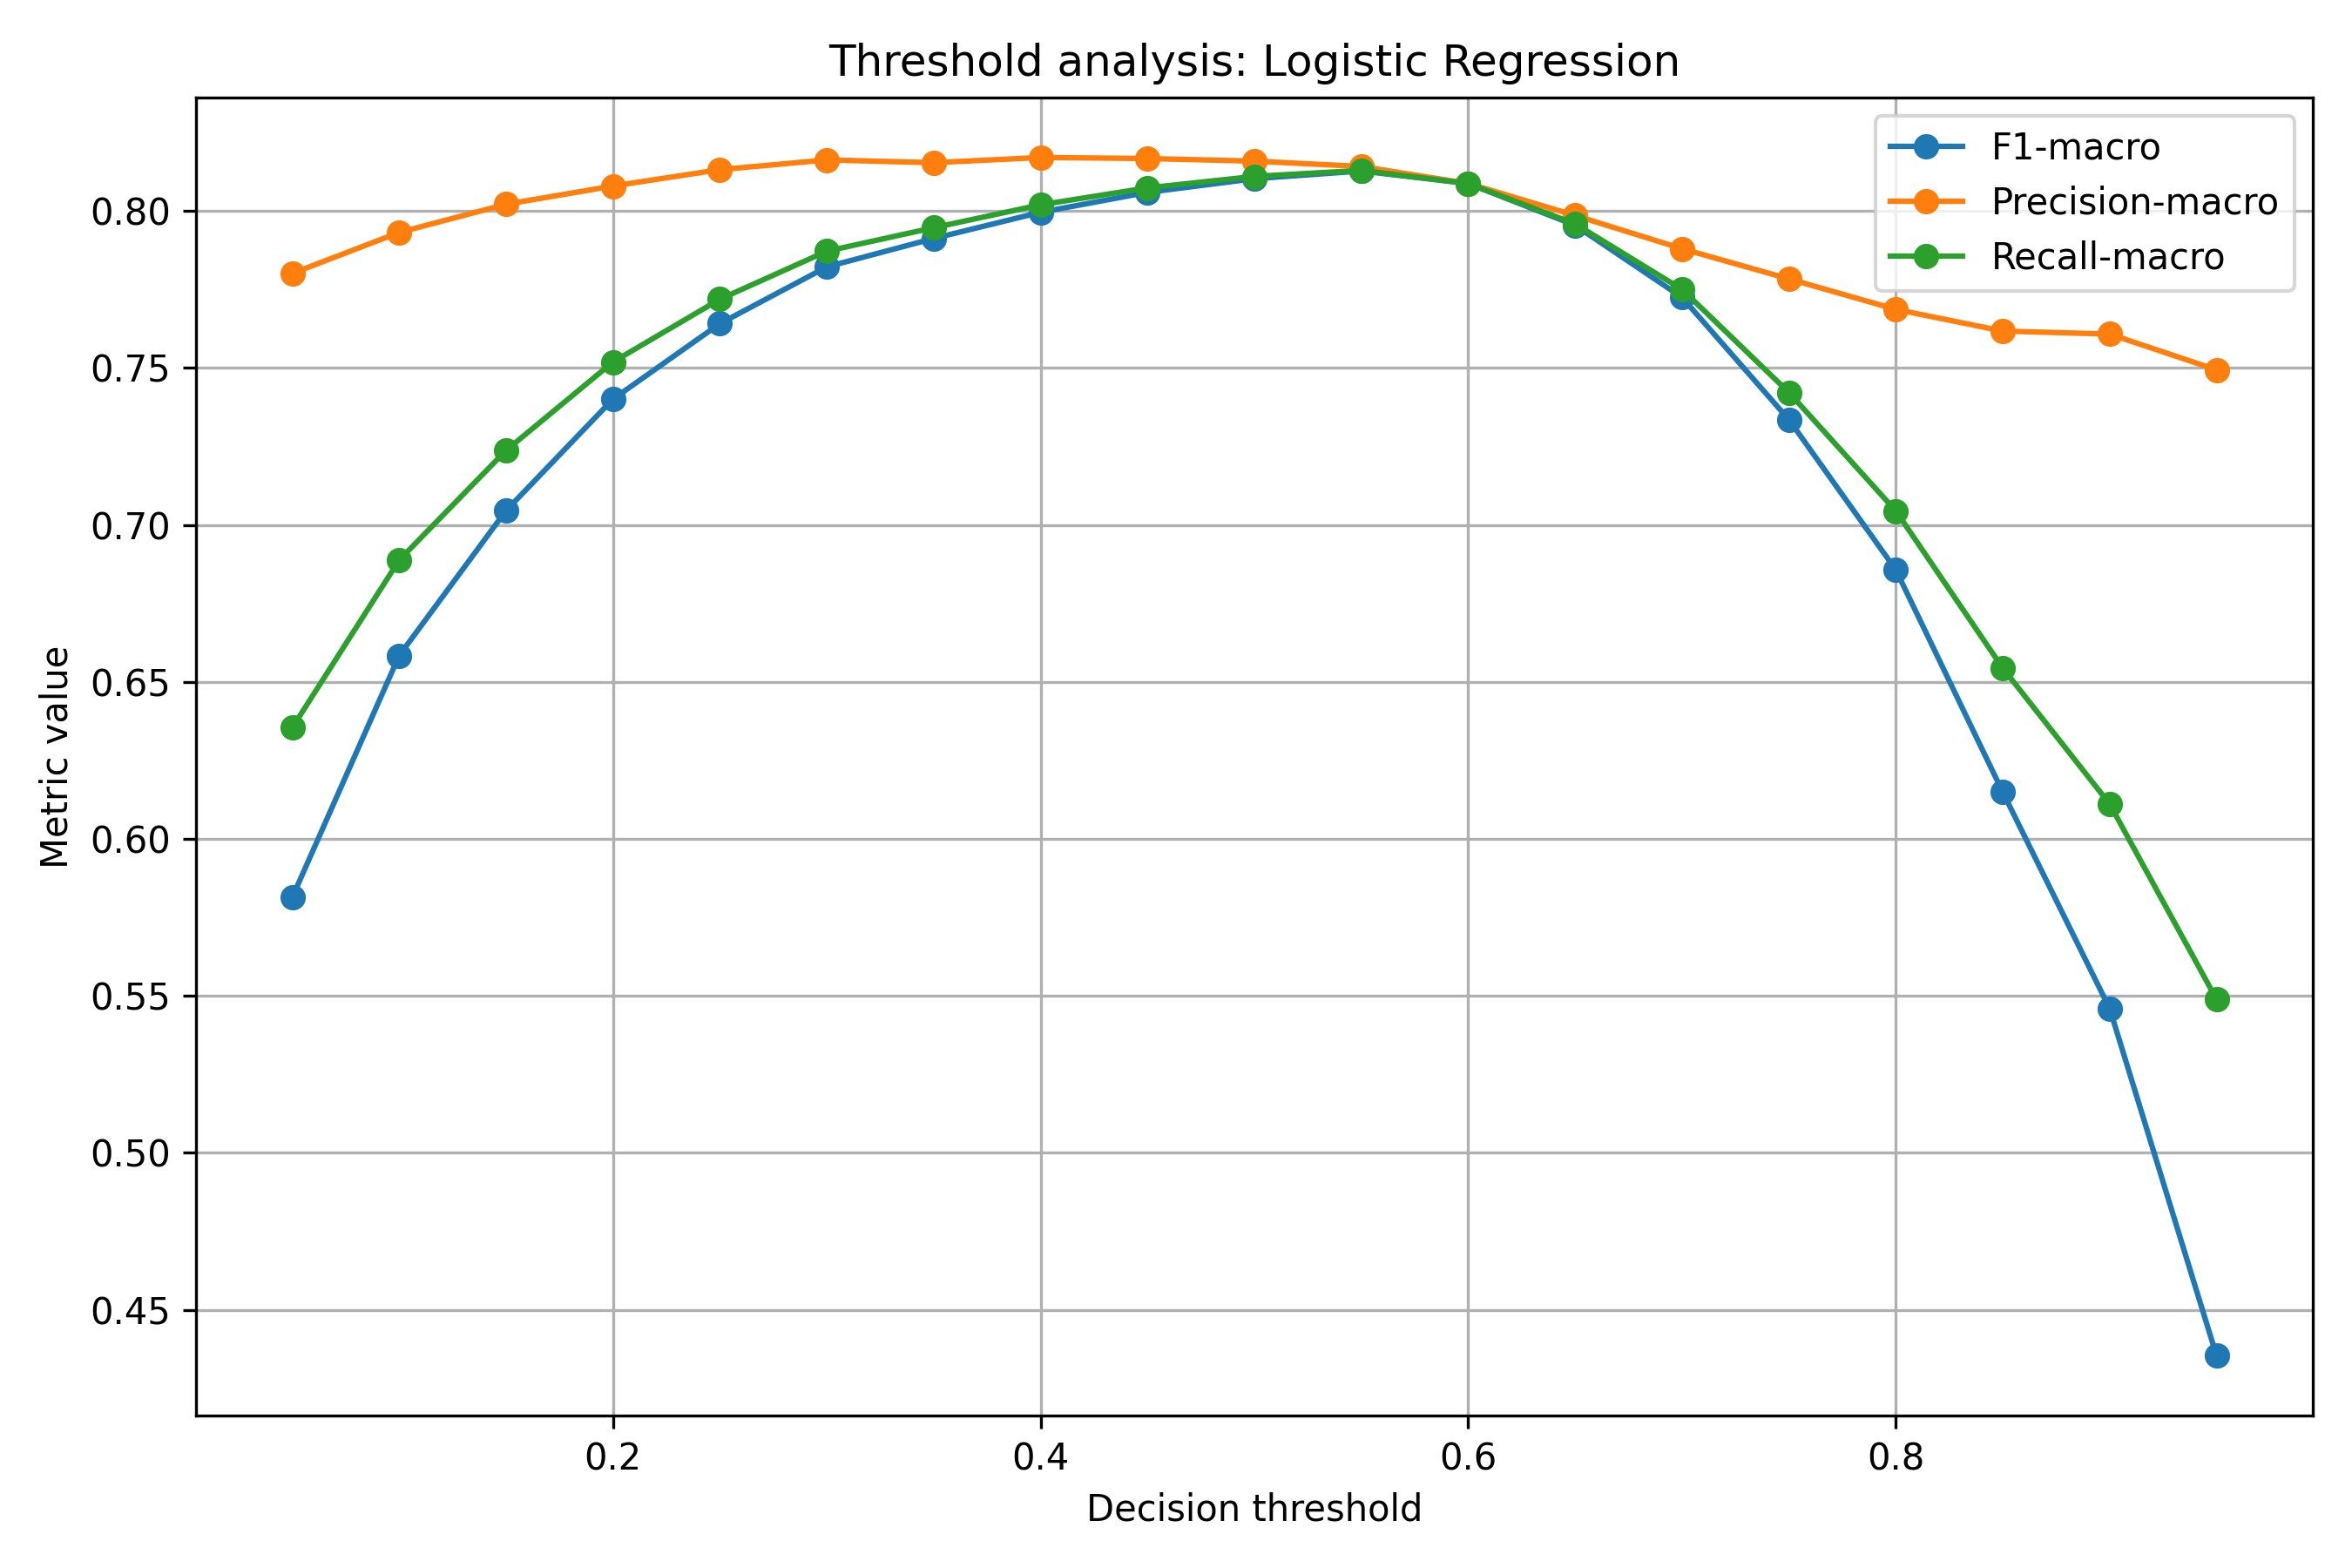
\includegraphics[width=0.82\textwidth]{logistic_regression_images/logistic_regression_threshold_analysis.png}
\caption{Анализ порога классификации: Logistic Regression}
\end{figure}
\begin{figure}[H]
\centering
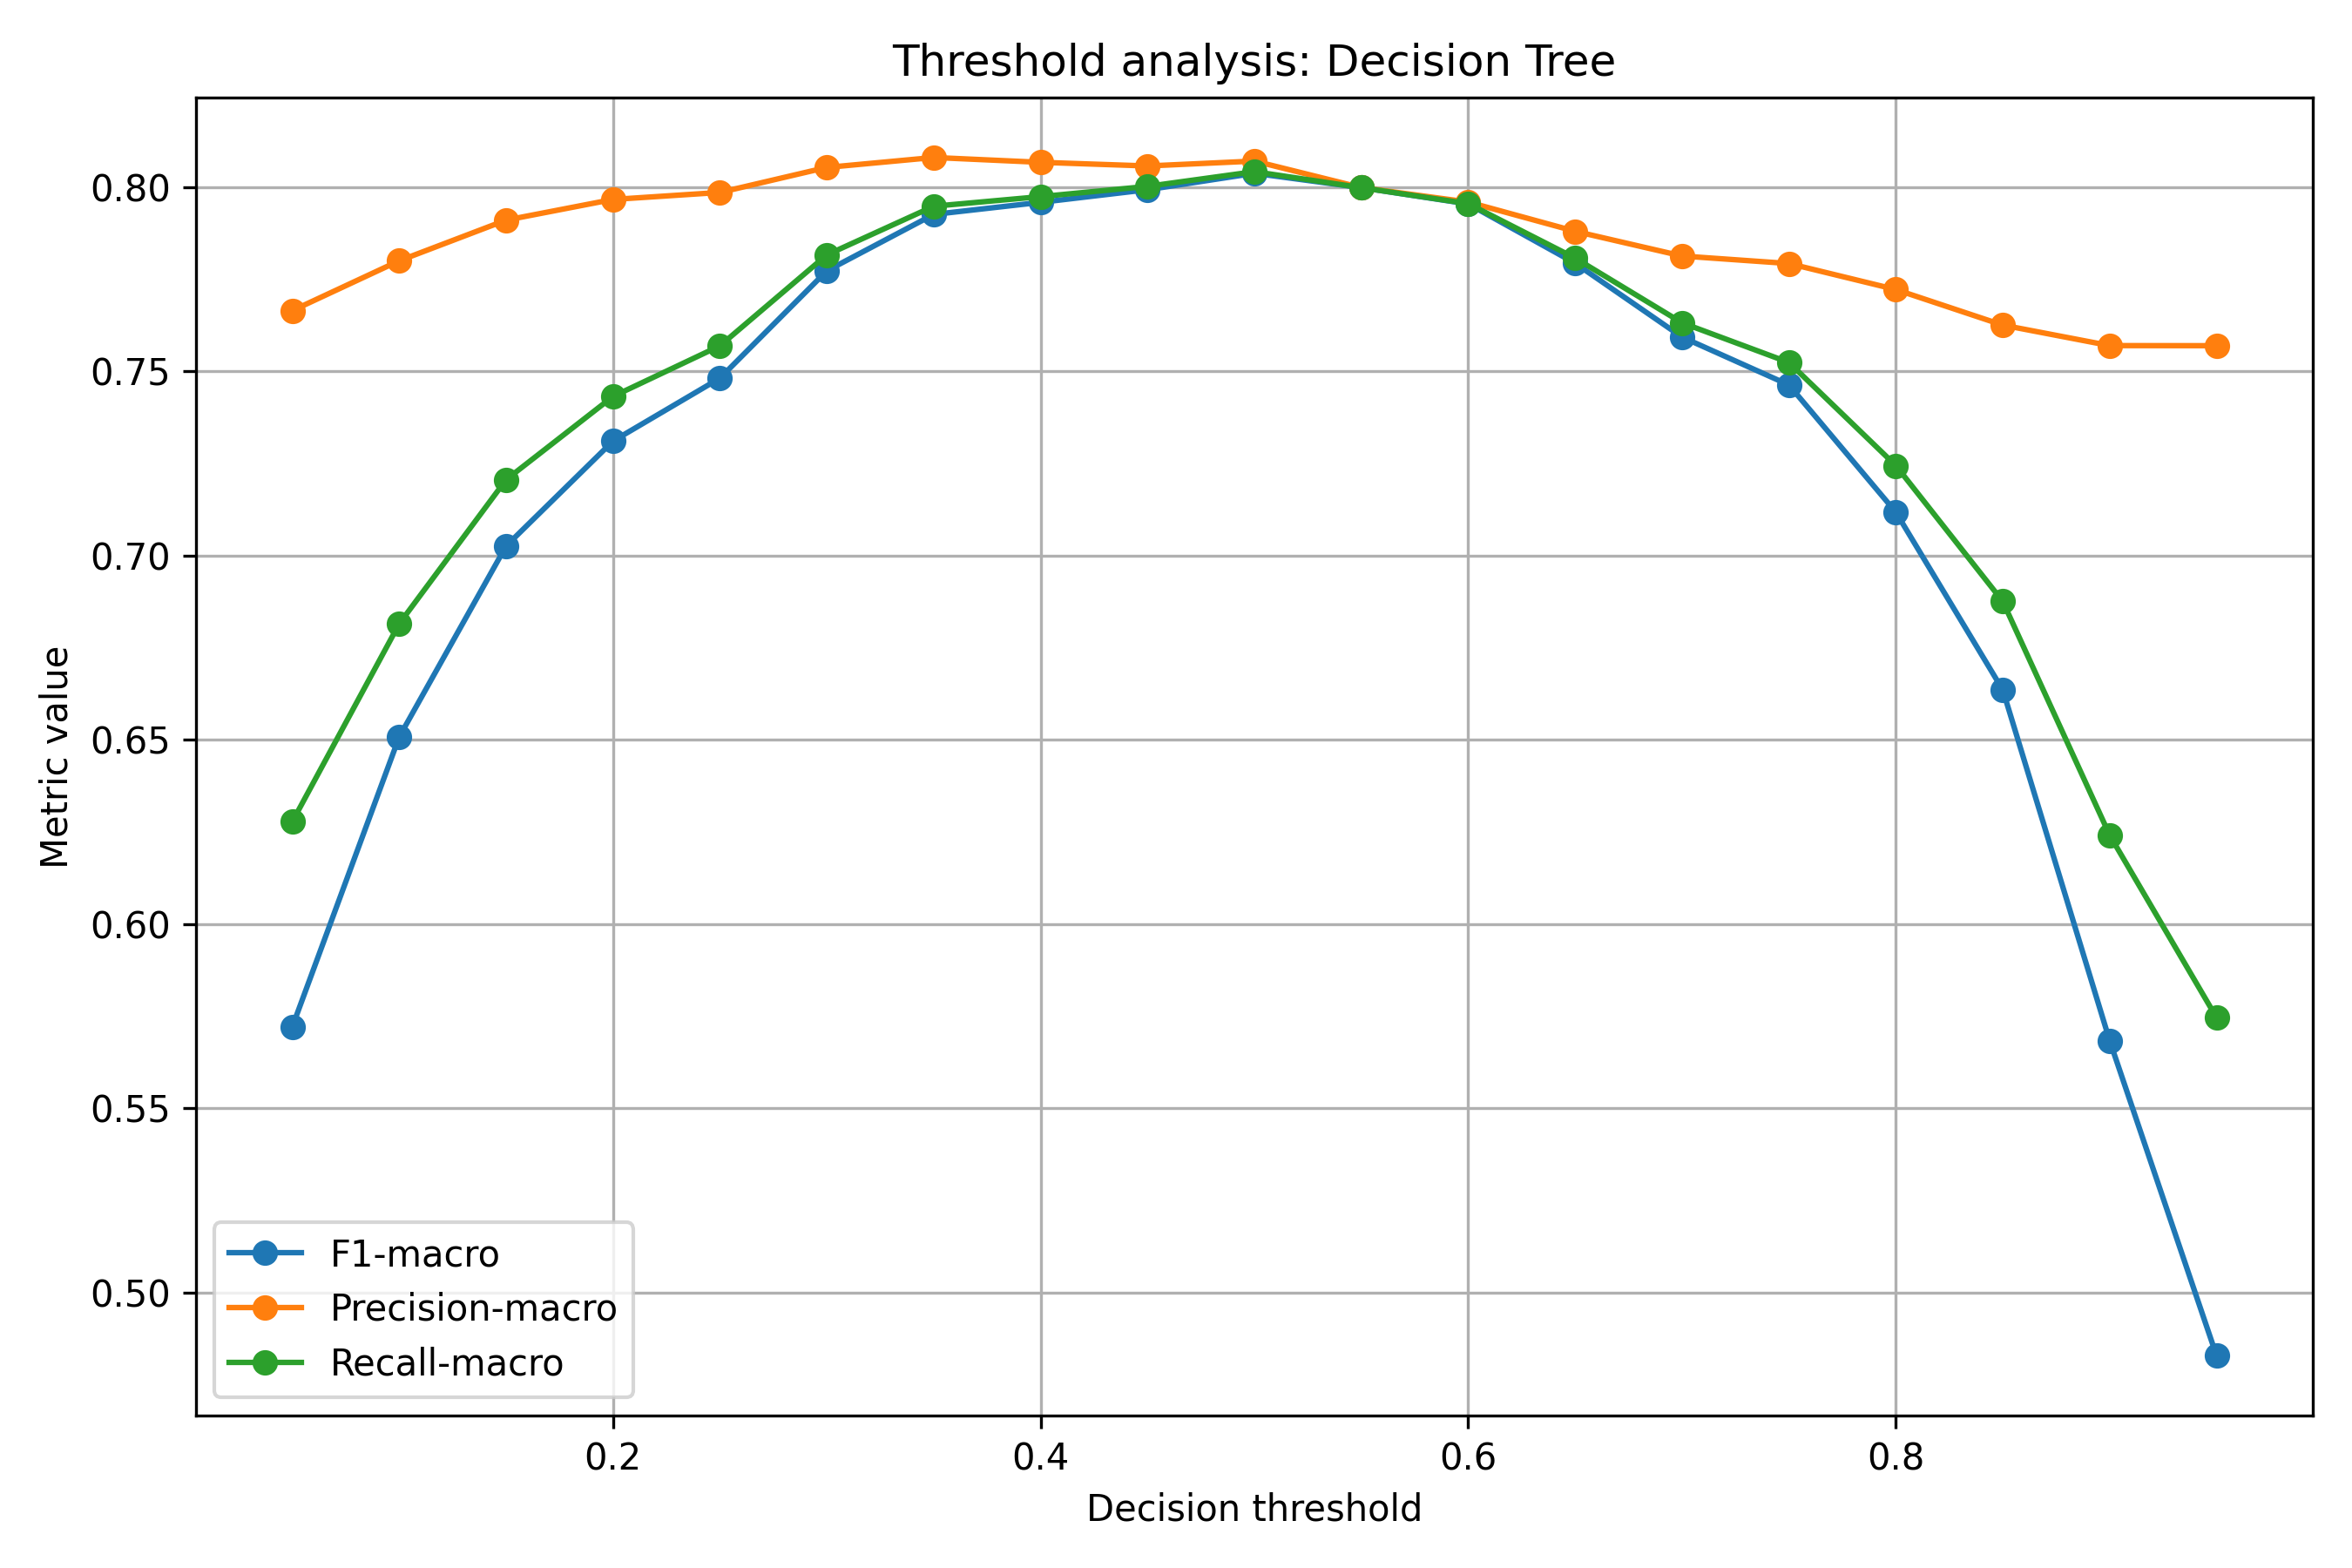
\includegraphics[width=0.82\textwidth]{decision_tree_images/decision_tree_threshold_analysis.png}
\caption{Анализ порога классификации: Decision Tree}
\end{figure}
\begin{figure}[H]
\centering
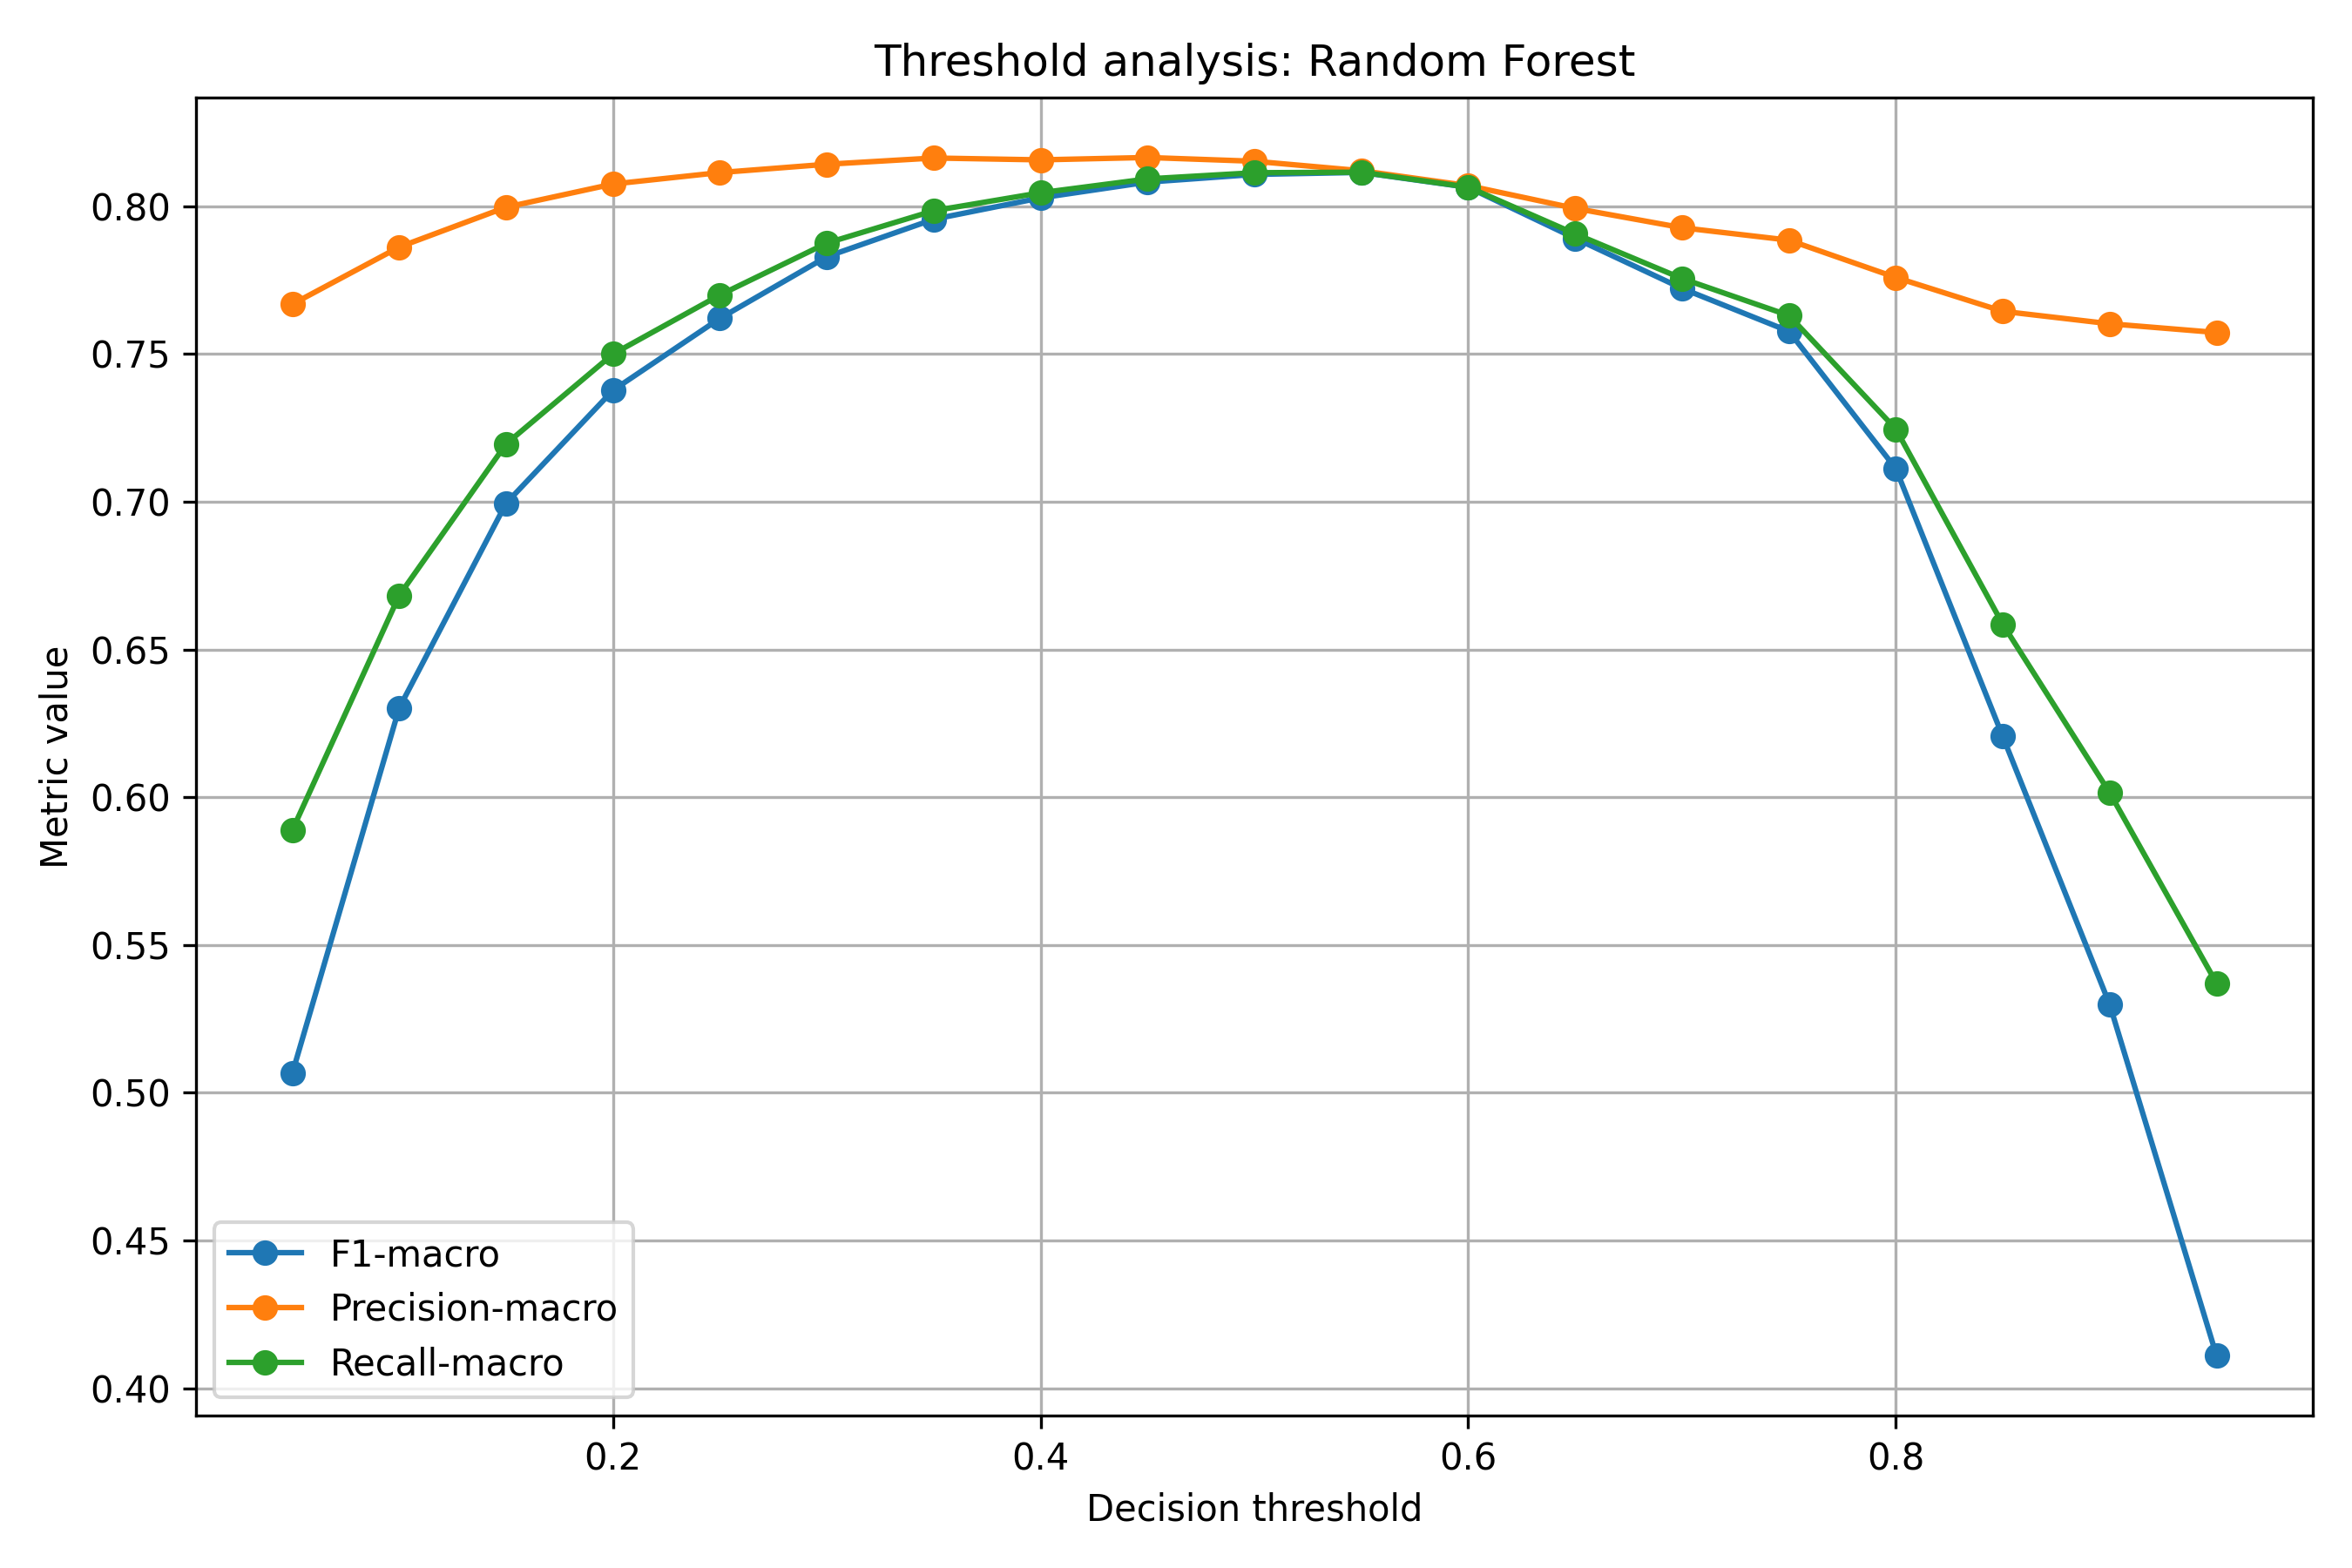
\includegraphics[width=0.82\textwidth]{random_forest_images/random_forest_threshold_analysis.png}
\caption{Анализ порога классификации: Random Forest}
\end{figure}
\begin{figure}[H]
\centering
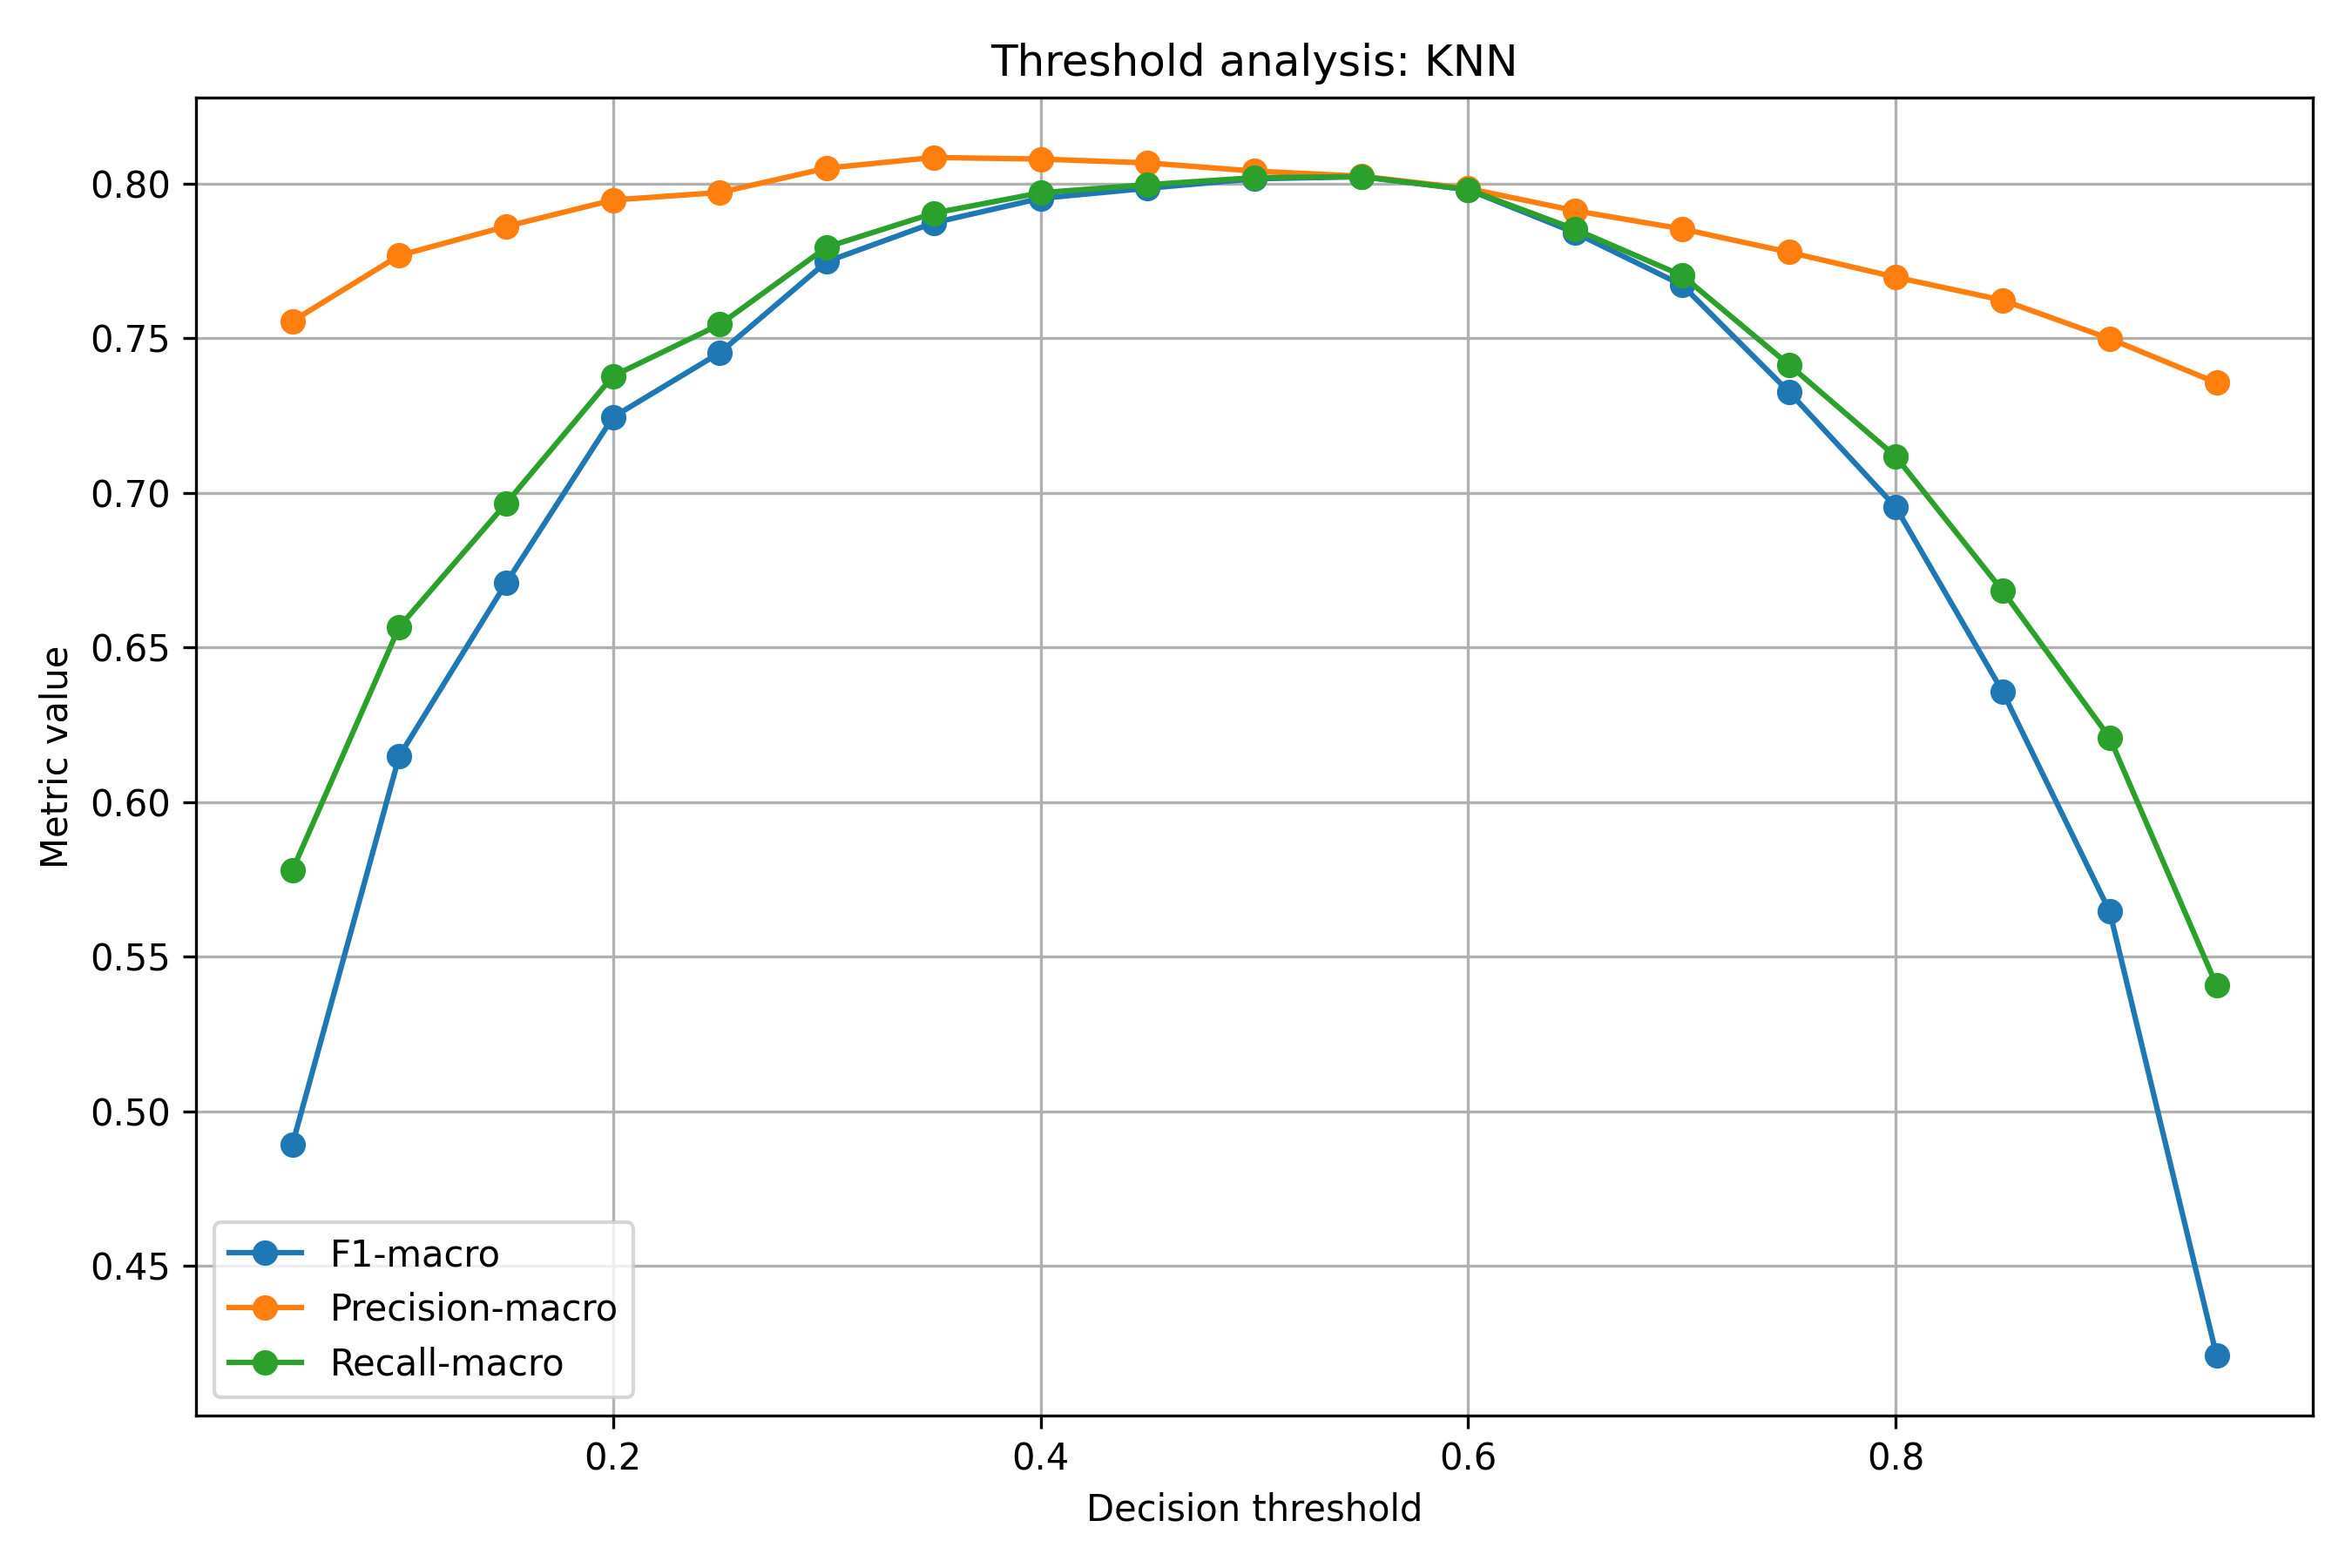
\includegraphics[width=0.82\textwidth]{knn_images/knn_threshold_analysis.png}
\caption{Анализ порога классификации: KNN}
\end{figure}
\begin{figure}[H]
\centering
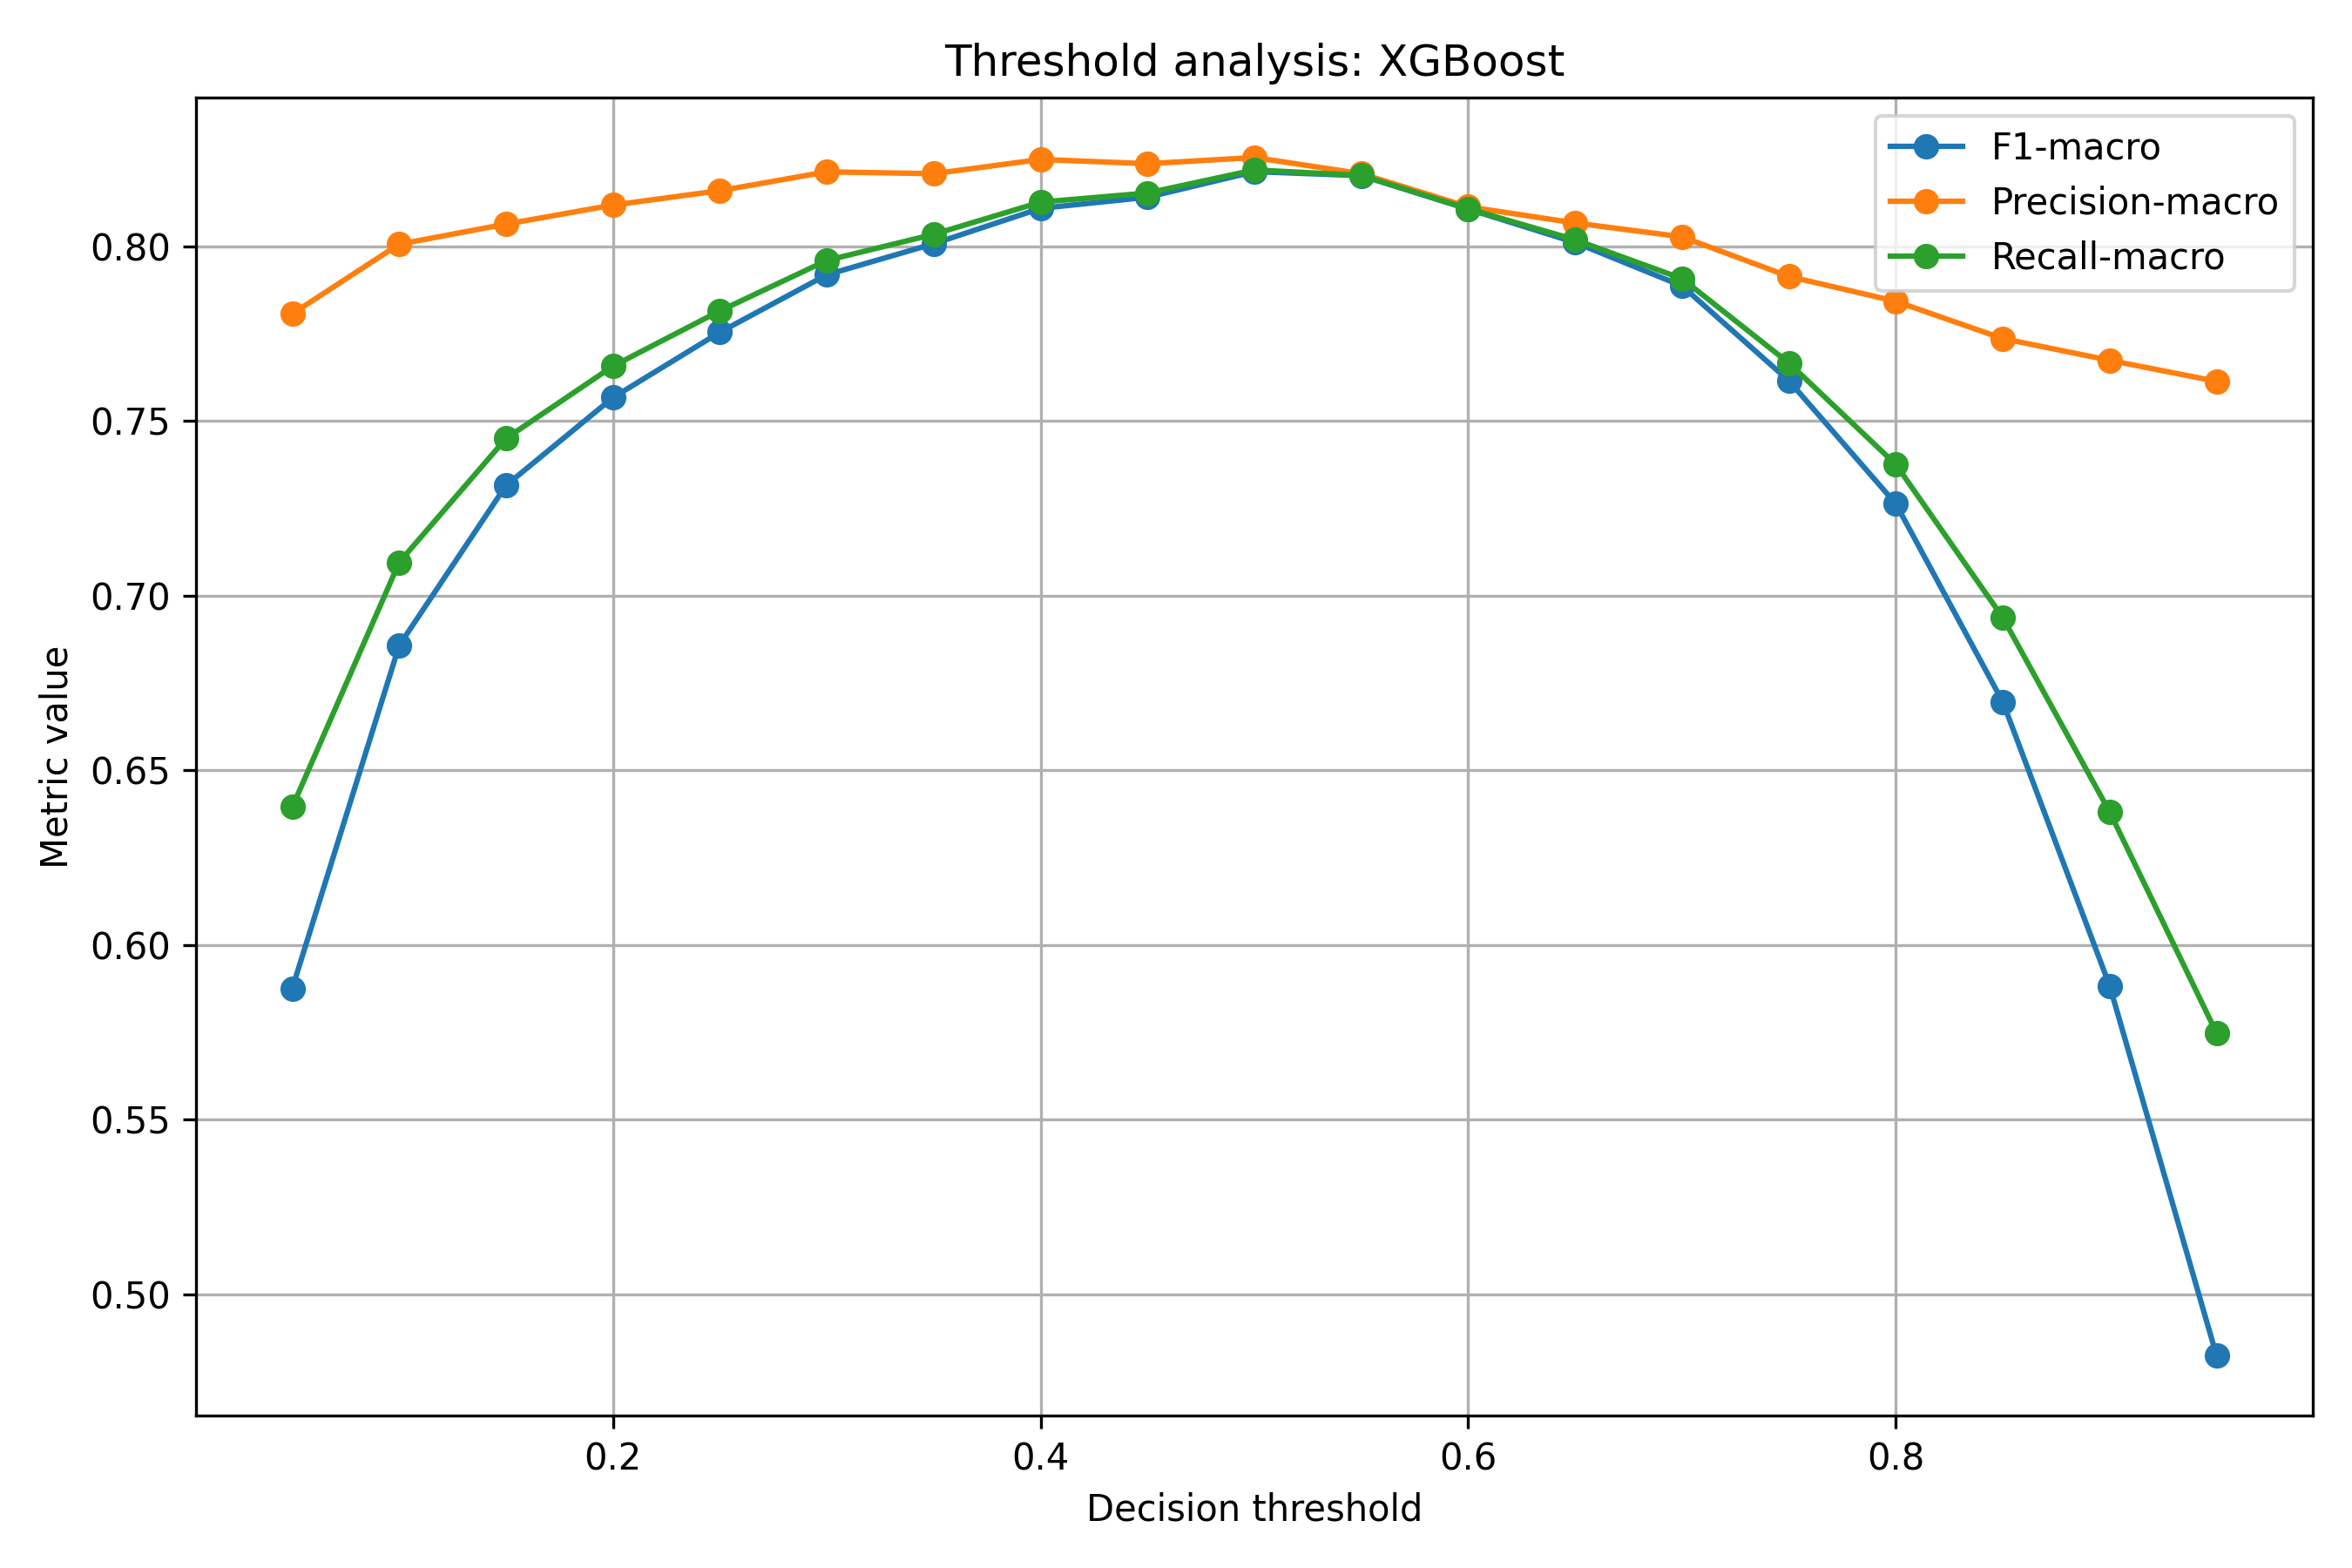
\includegraphics[width=0.82\textwidth]{xgboost_images/xgboost_threshold_analysis.png}
\caption{Анализ порога классификации: XGBoost}
\end{figure}
\begin{figure}[H]
\centering
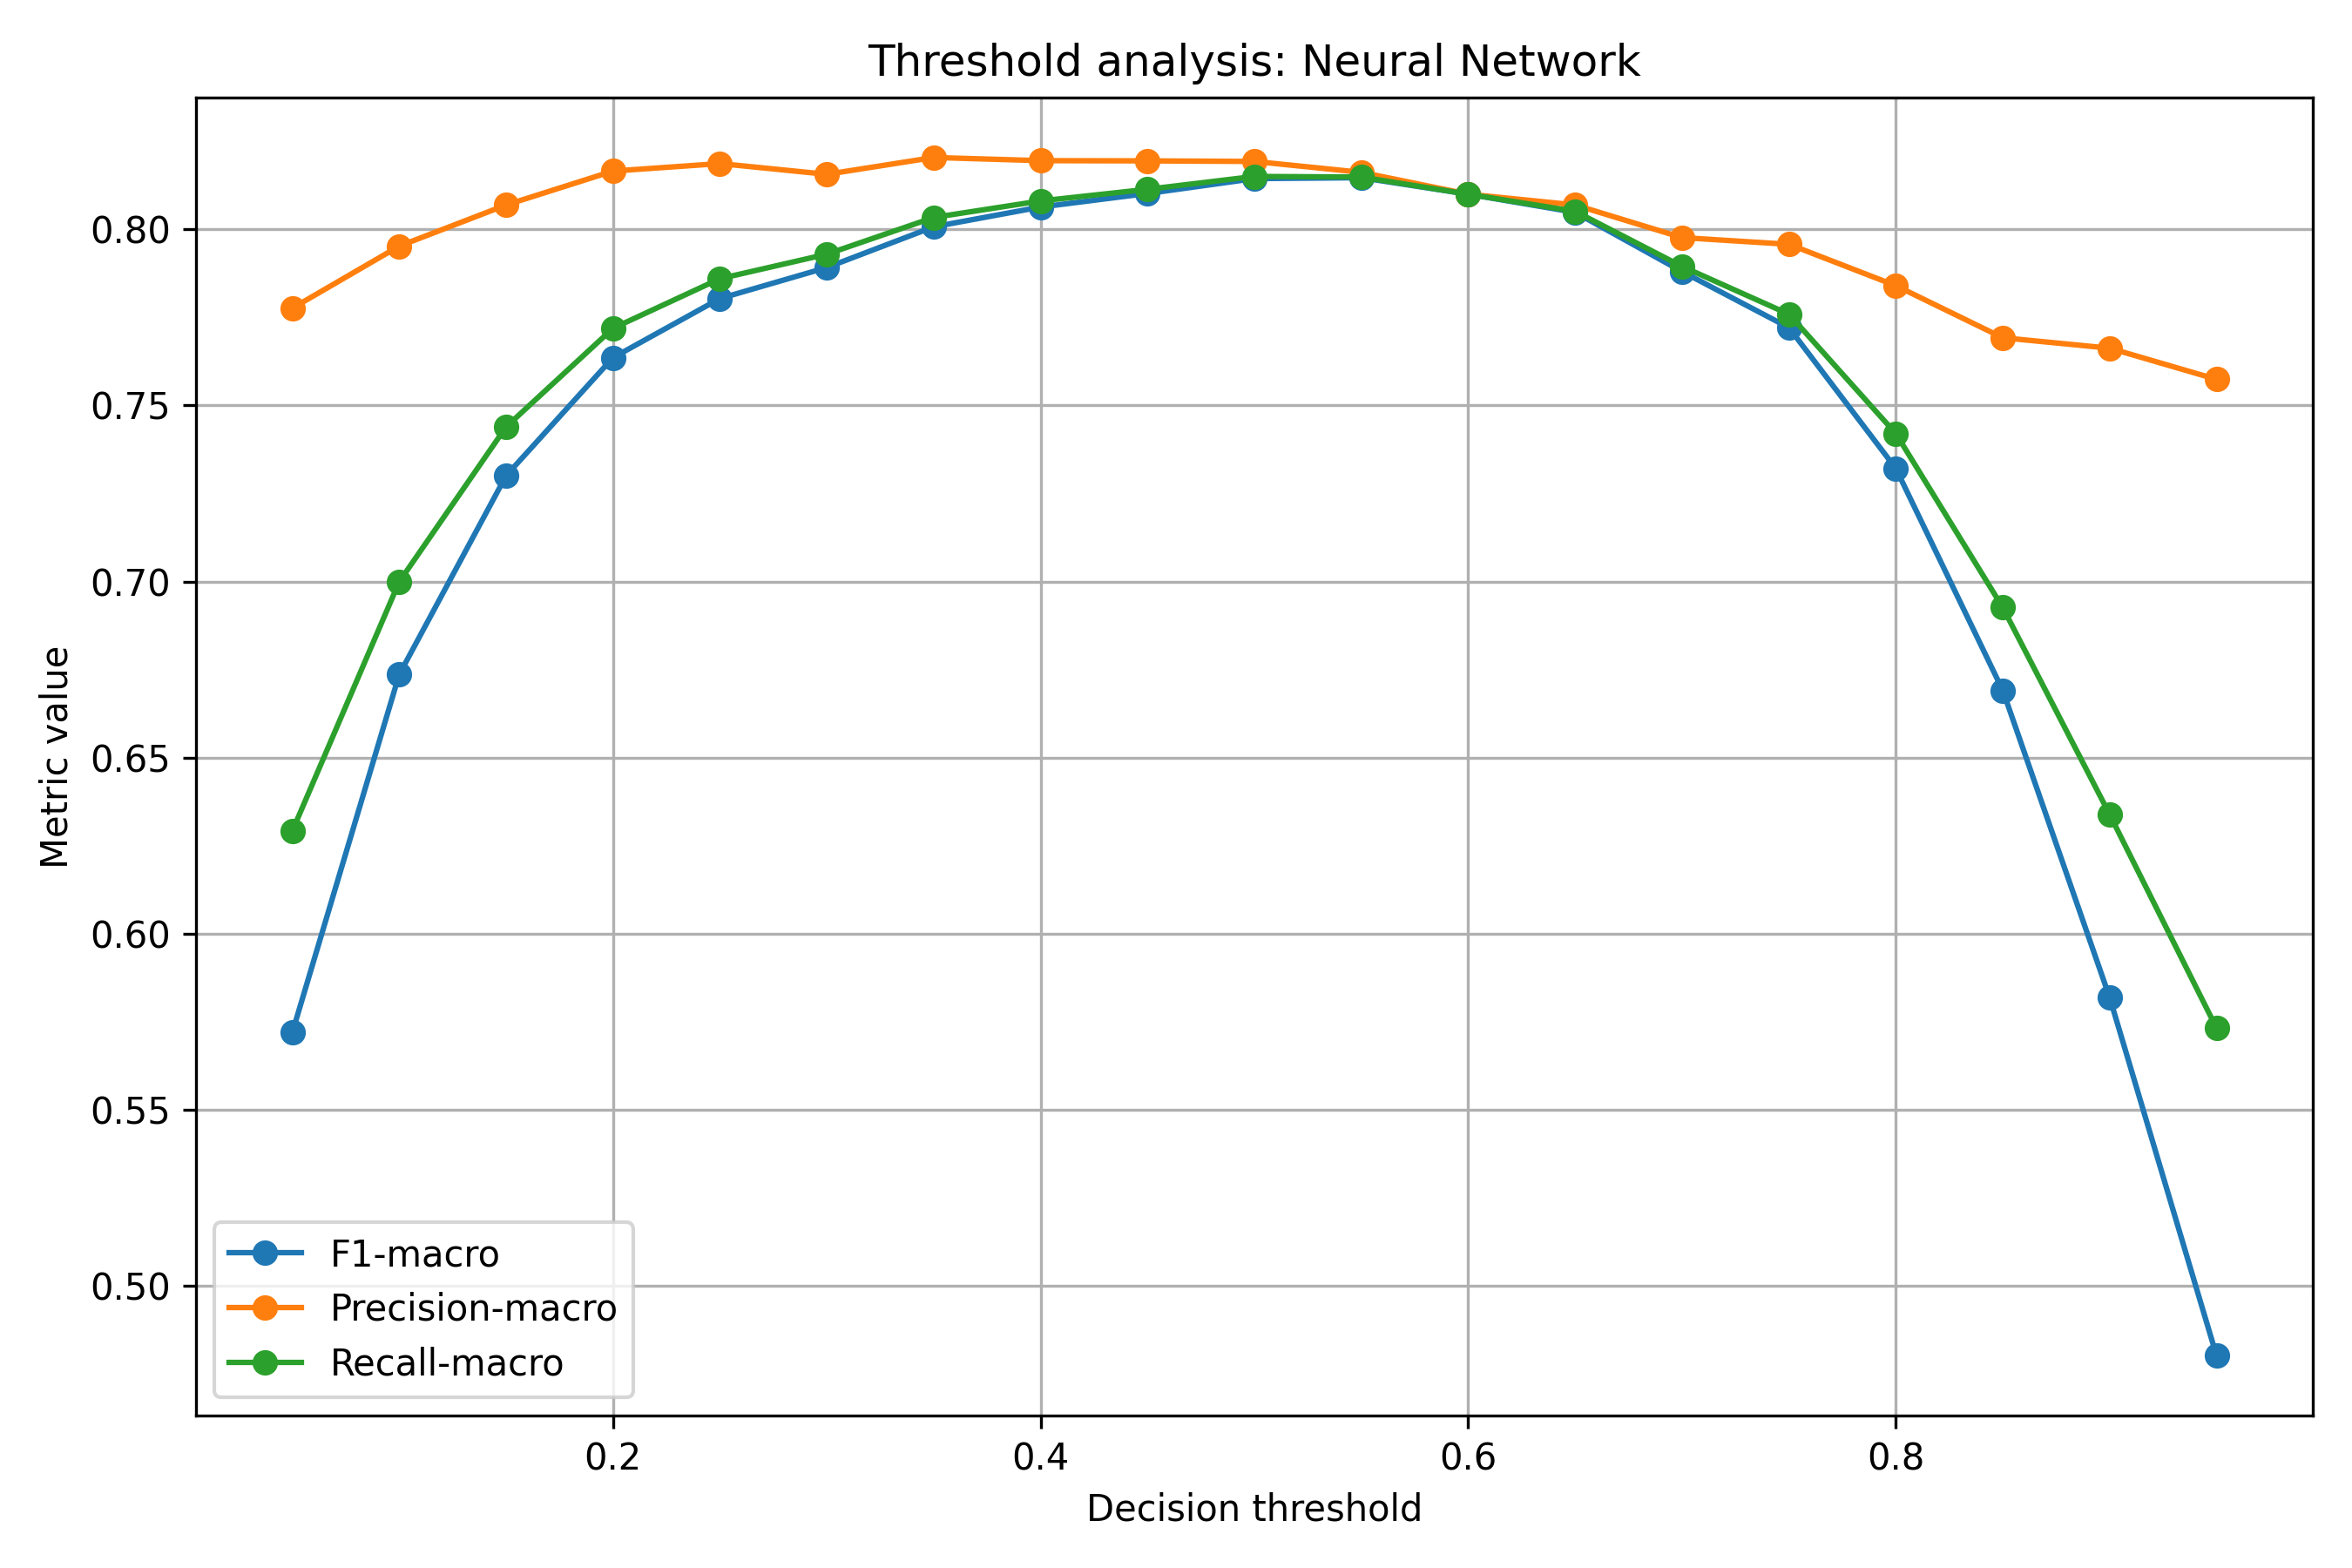
\includegraphics[width=0.82\textwidth]{neural_network_images/neural_network_threshold_analysis.png}
\caption{Анализ порога классификации: Neural Network}
\end{figure}

Анализ порога классификации показывает, что стандартный порог 0.5 не всегда является оптимальным. Для Logistic Regression и KNN лучший F1-macro достигается при пороге 0.55, то есть этим моделям полезно немного строже относиться к положительному классу. Для Decision Tree, Random Forest, XGBoost и Neural Network оптимальным в проведенном эксперименте остался порог 0.5. Изменение порога позволяет управлять компромиссом между sensitivity и specificity, что особенно важно при практическом использовании модели для раннего выявления неудовлетворенных клиентов. Если компании важнее не пропустить недовольного пассажира, порог можно снижать, принимая рост false positive как плату за более высокий recall проблемных случаев.

\section{Устойчивость к шуму}

\scriptsize
\begin{longtable}{llllll}
\caption{Сводка robustness check}\label{tab:robustness}\\
\toprule
Модель & Baseline F1 & Худший тест & Уровень & F1 при искажении & Падение F1 \\
\midrule
\endfirsthead
\toprule
Модель & Baseline F1 & Худший тест & Уровень & F1 при искажении & Падение F1 \\
\midrule
\endhead
Logistic Regression & 0.810 & missing\_values & 0.05 & 0.795 & 0.015 \\
Decision Tree & 0.804 & missing\_values & 0.05 & 0.796 & 0.008 \\
Random Forest & 0.810 & missing\_values & 0.05 & 0.808 & 0.002 \\
KNN & 0.800 & missing\_values & 0.05 & 0.796 & 0.004 \\
XGBoost & 0.821 & numeric\_noise & 0.10 & 0.753 & 0.068 \\
Neural Network & 0.814 & missing\_values & 0.05 & 0.798 & 0.016 \\
\bottomrule
\end{longtable}
\normalsize
\begin{figure}[H]
\centering
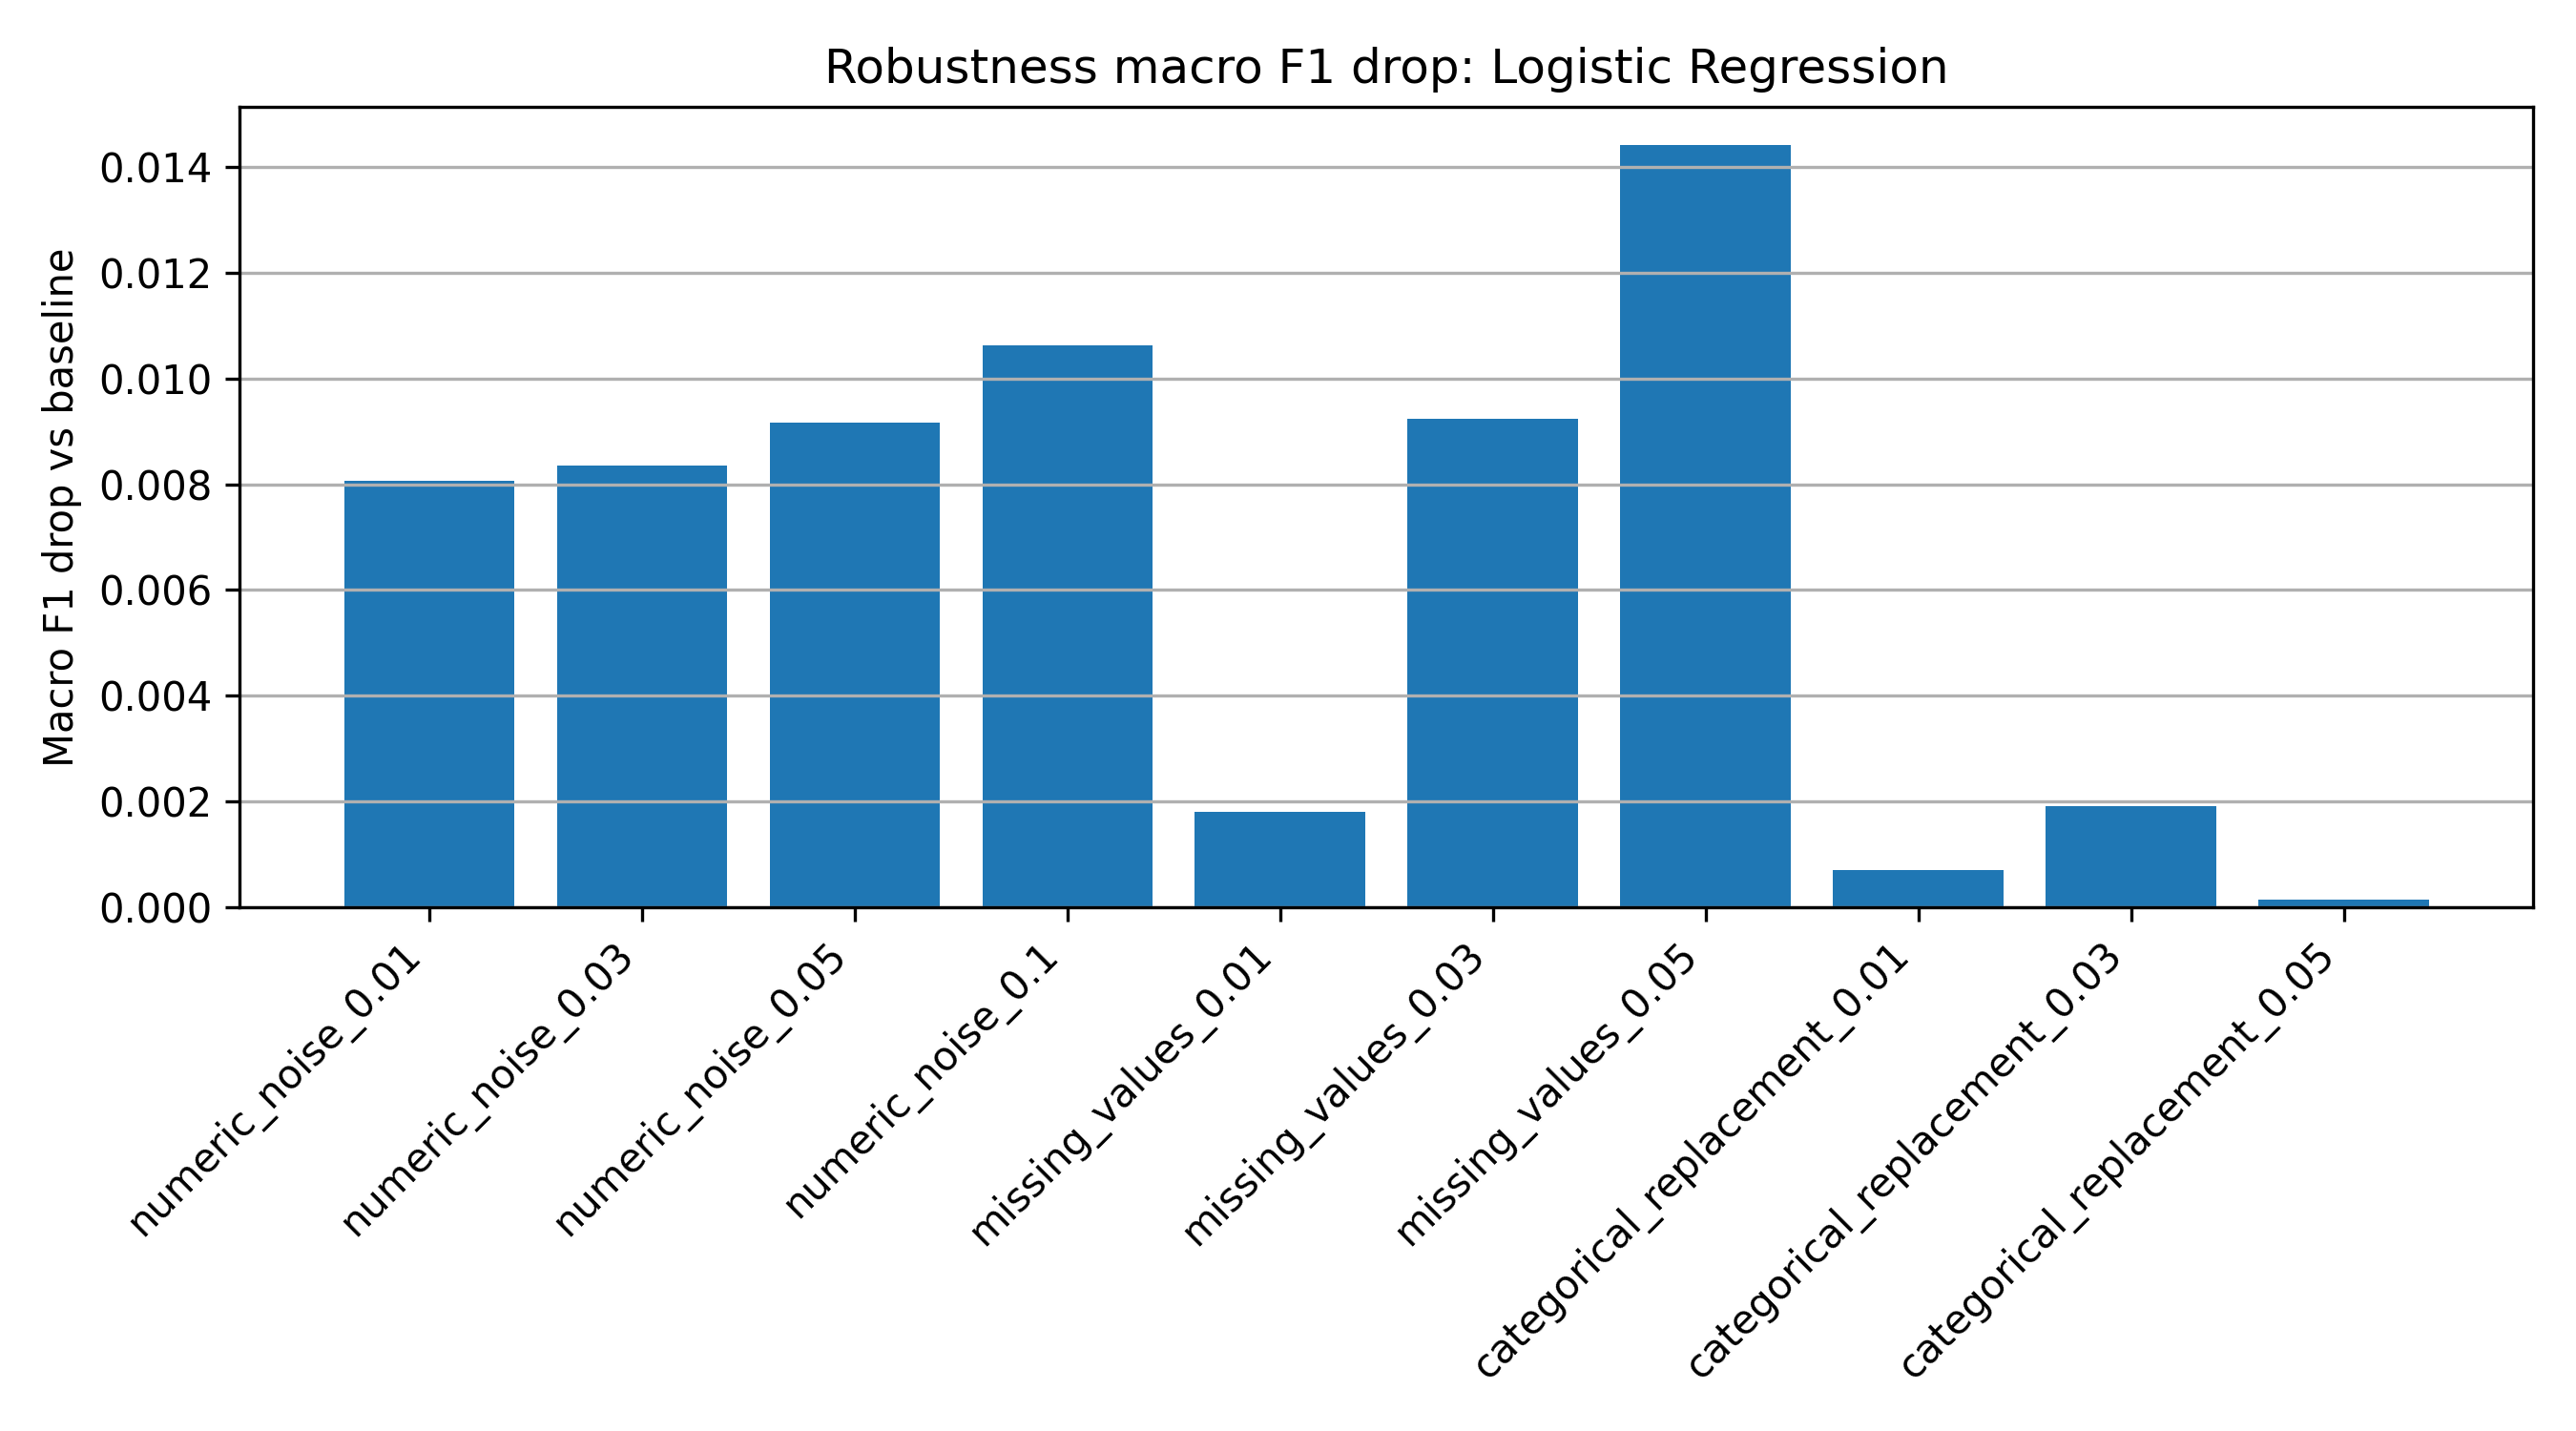
\includegraphics[width=0.82\textwidth]{logistic_regression_images/logistic_regression_robustness_f1_drop.png}
\caption{Падение F1-macro при искажениях: Logistic Regression}
\end{figure}
\begin{figure}[H]
\centering
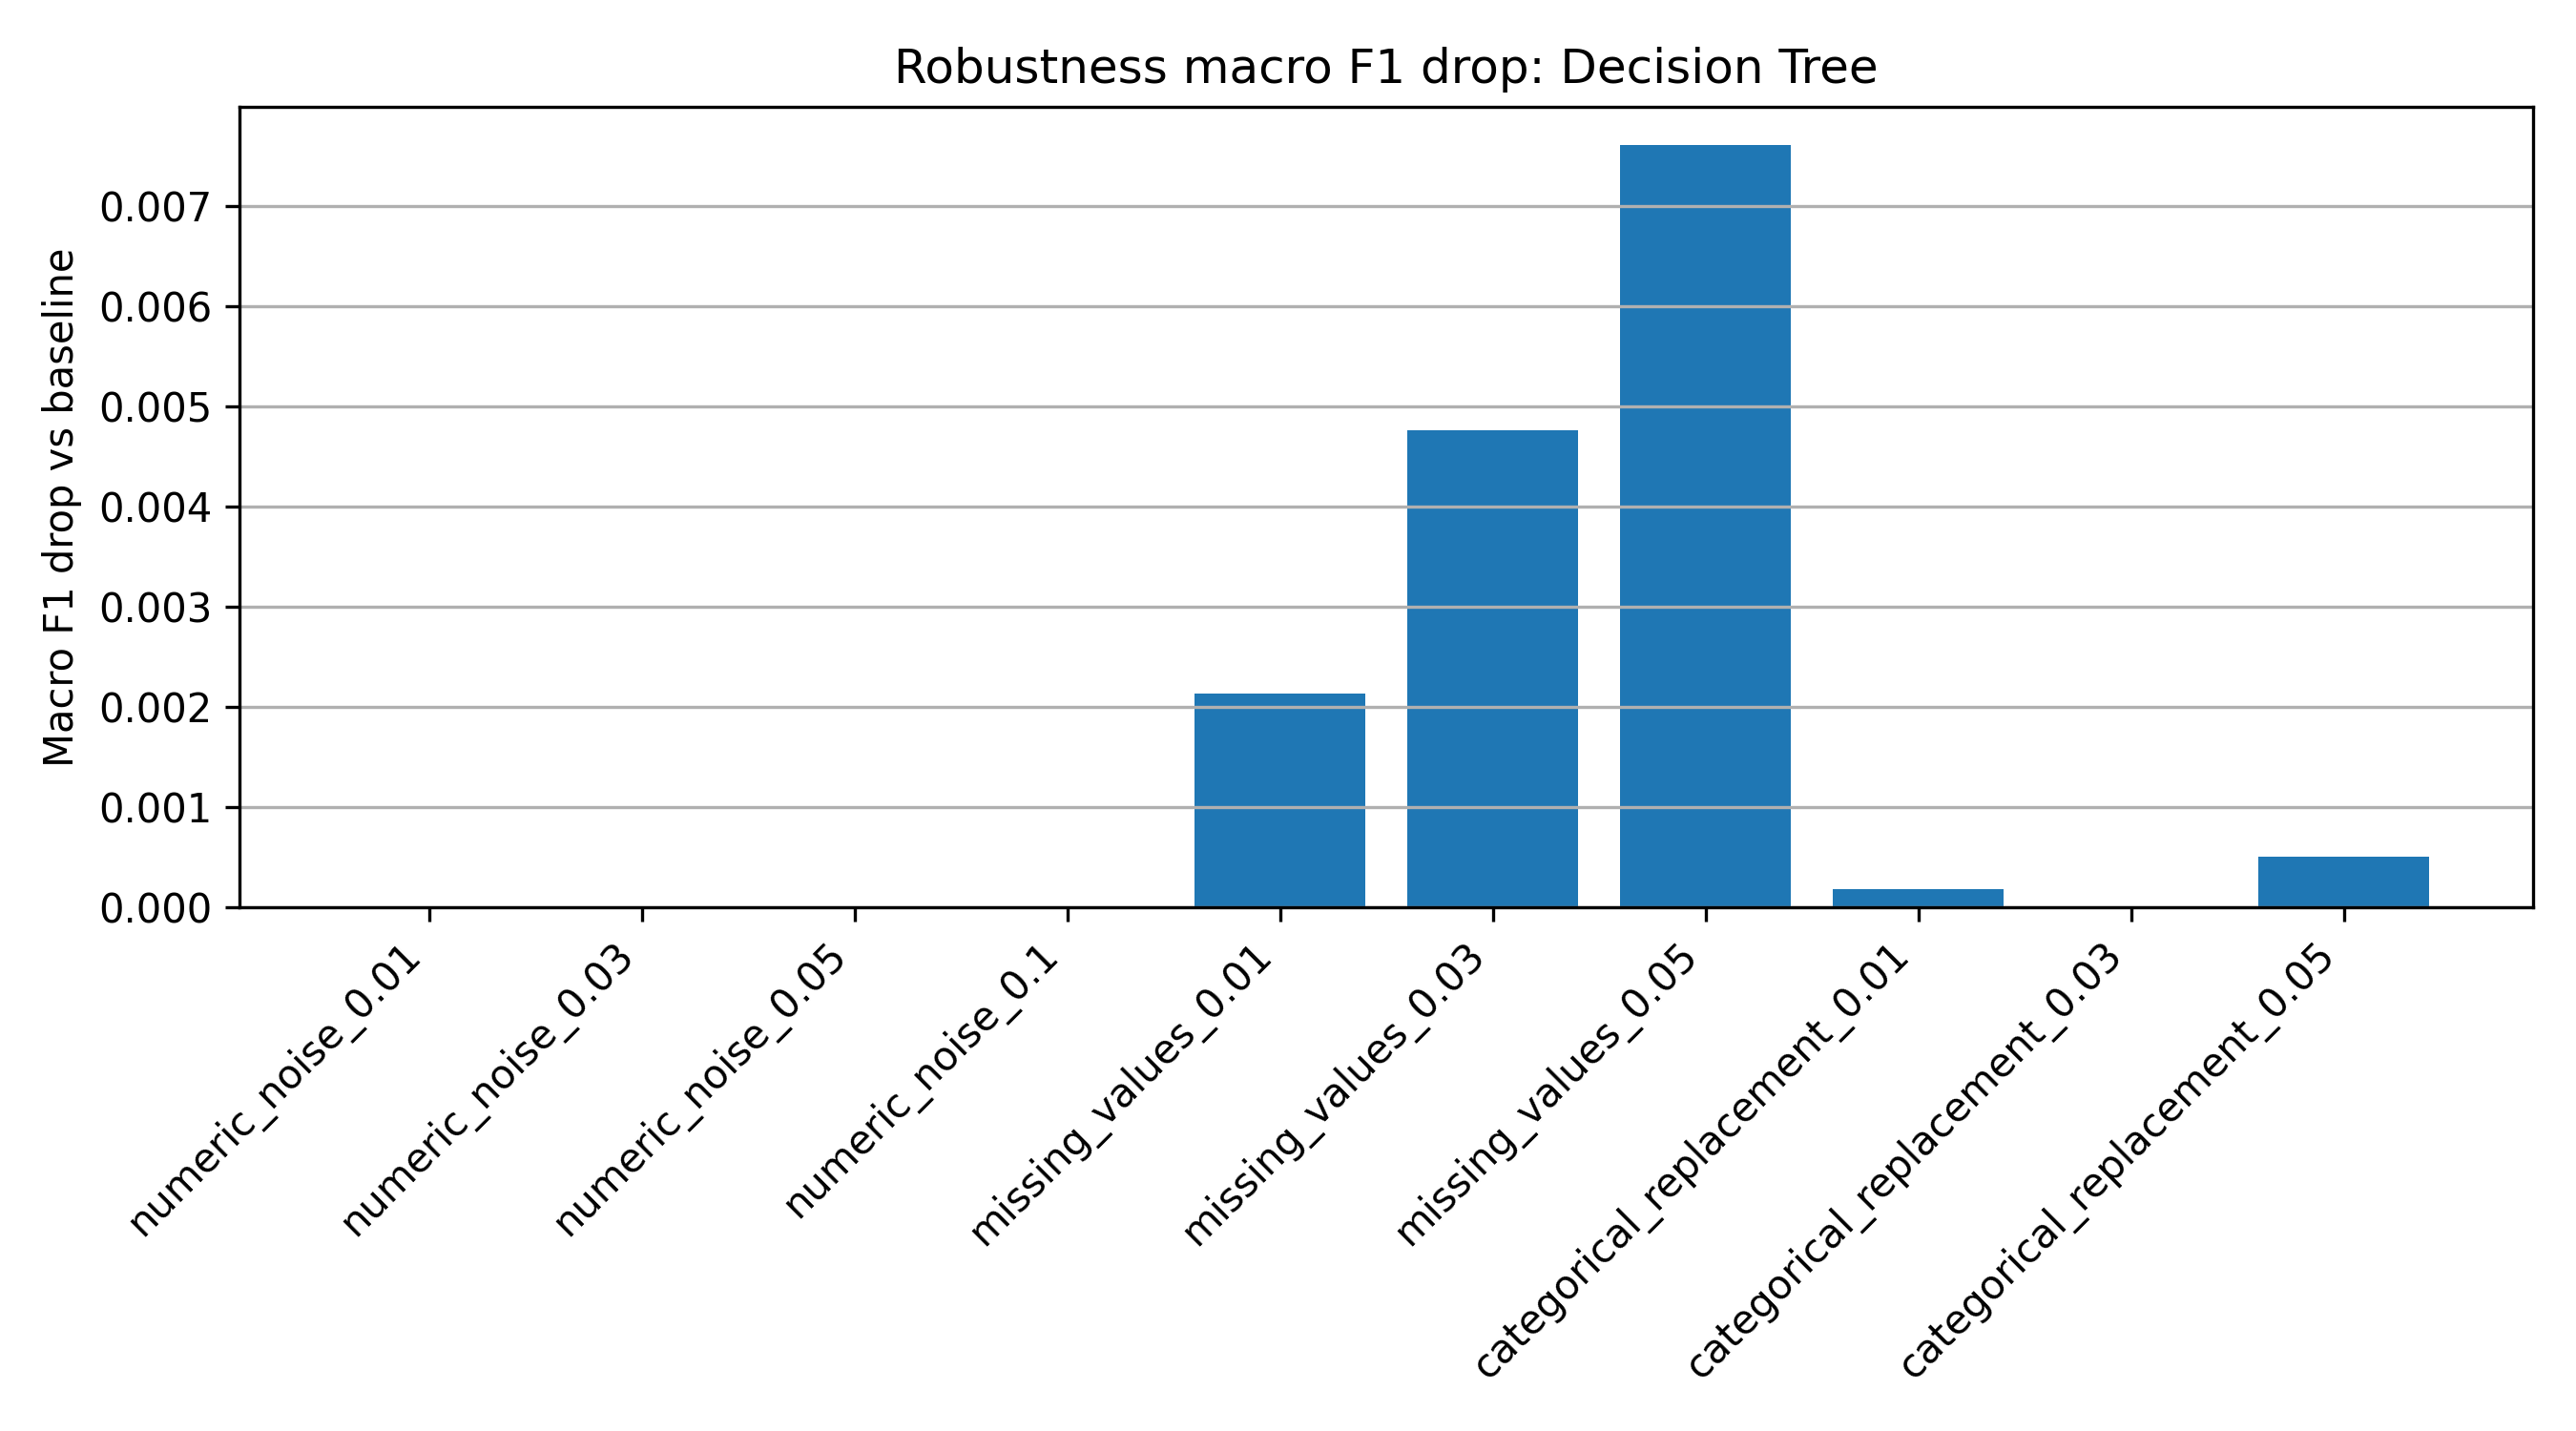
\includegraphics[width=0.82\textwidth]{decision_tree_images/decision_tree_robustness_f1_drop.png}
\caption{Падение F1-macro при искажениях: Decision Tree}
\end{figure}
\begin{figure}[H]
\centering
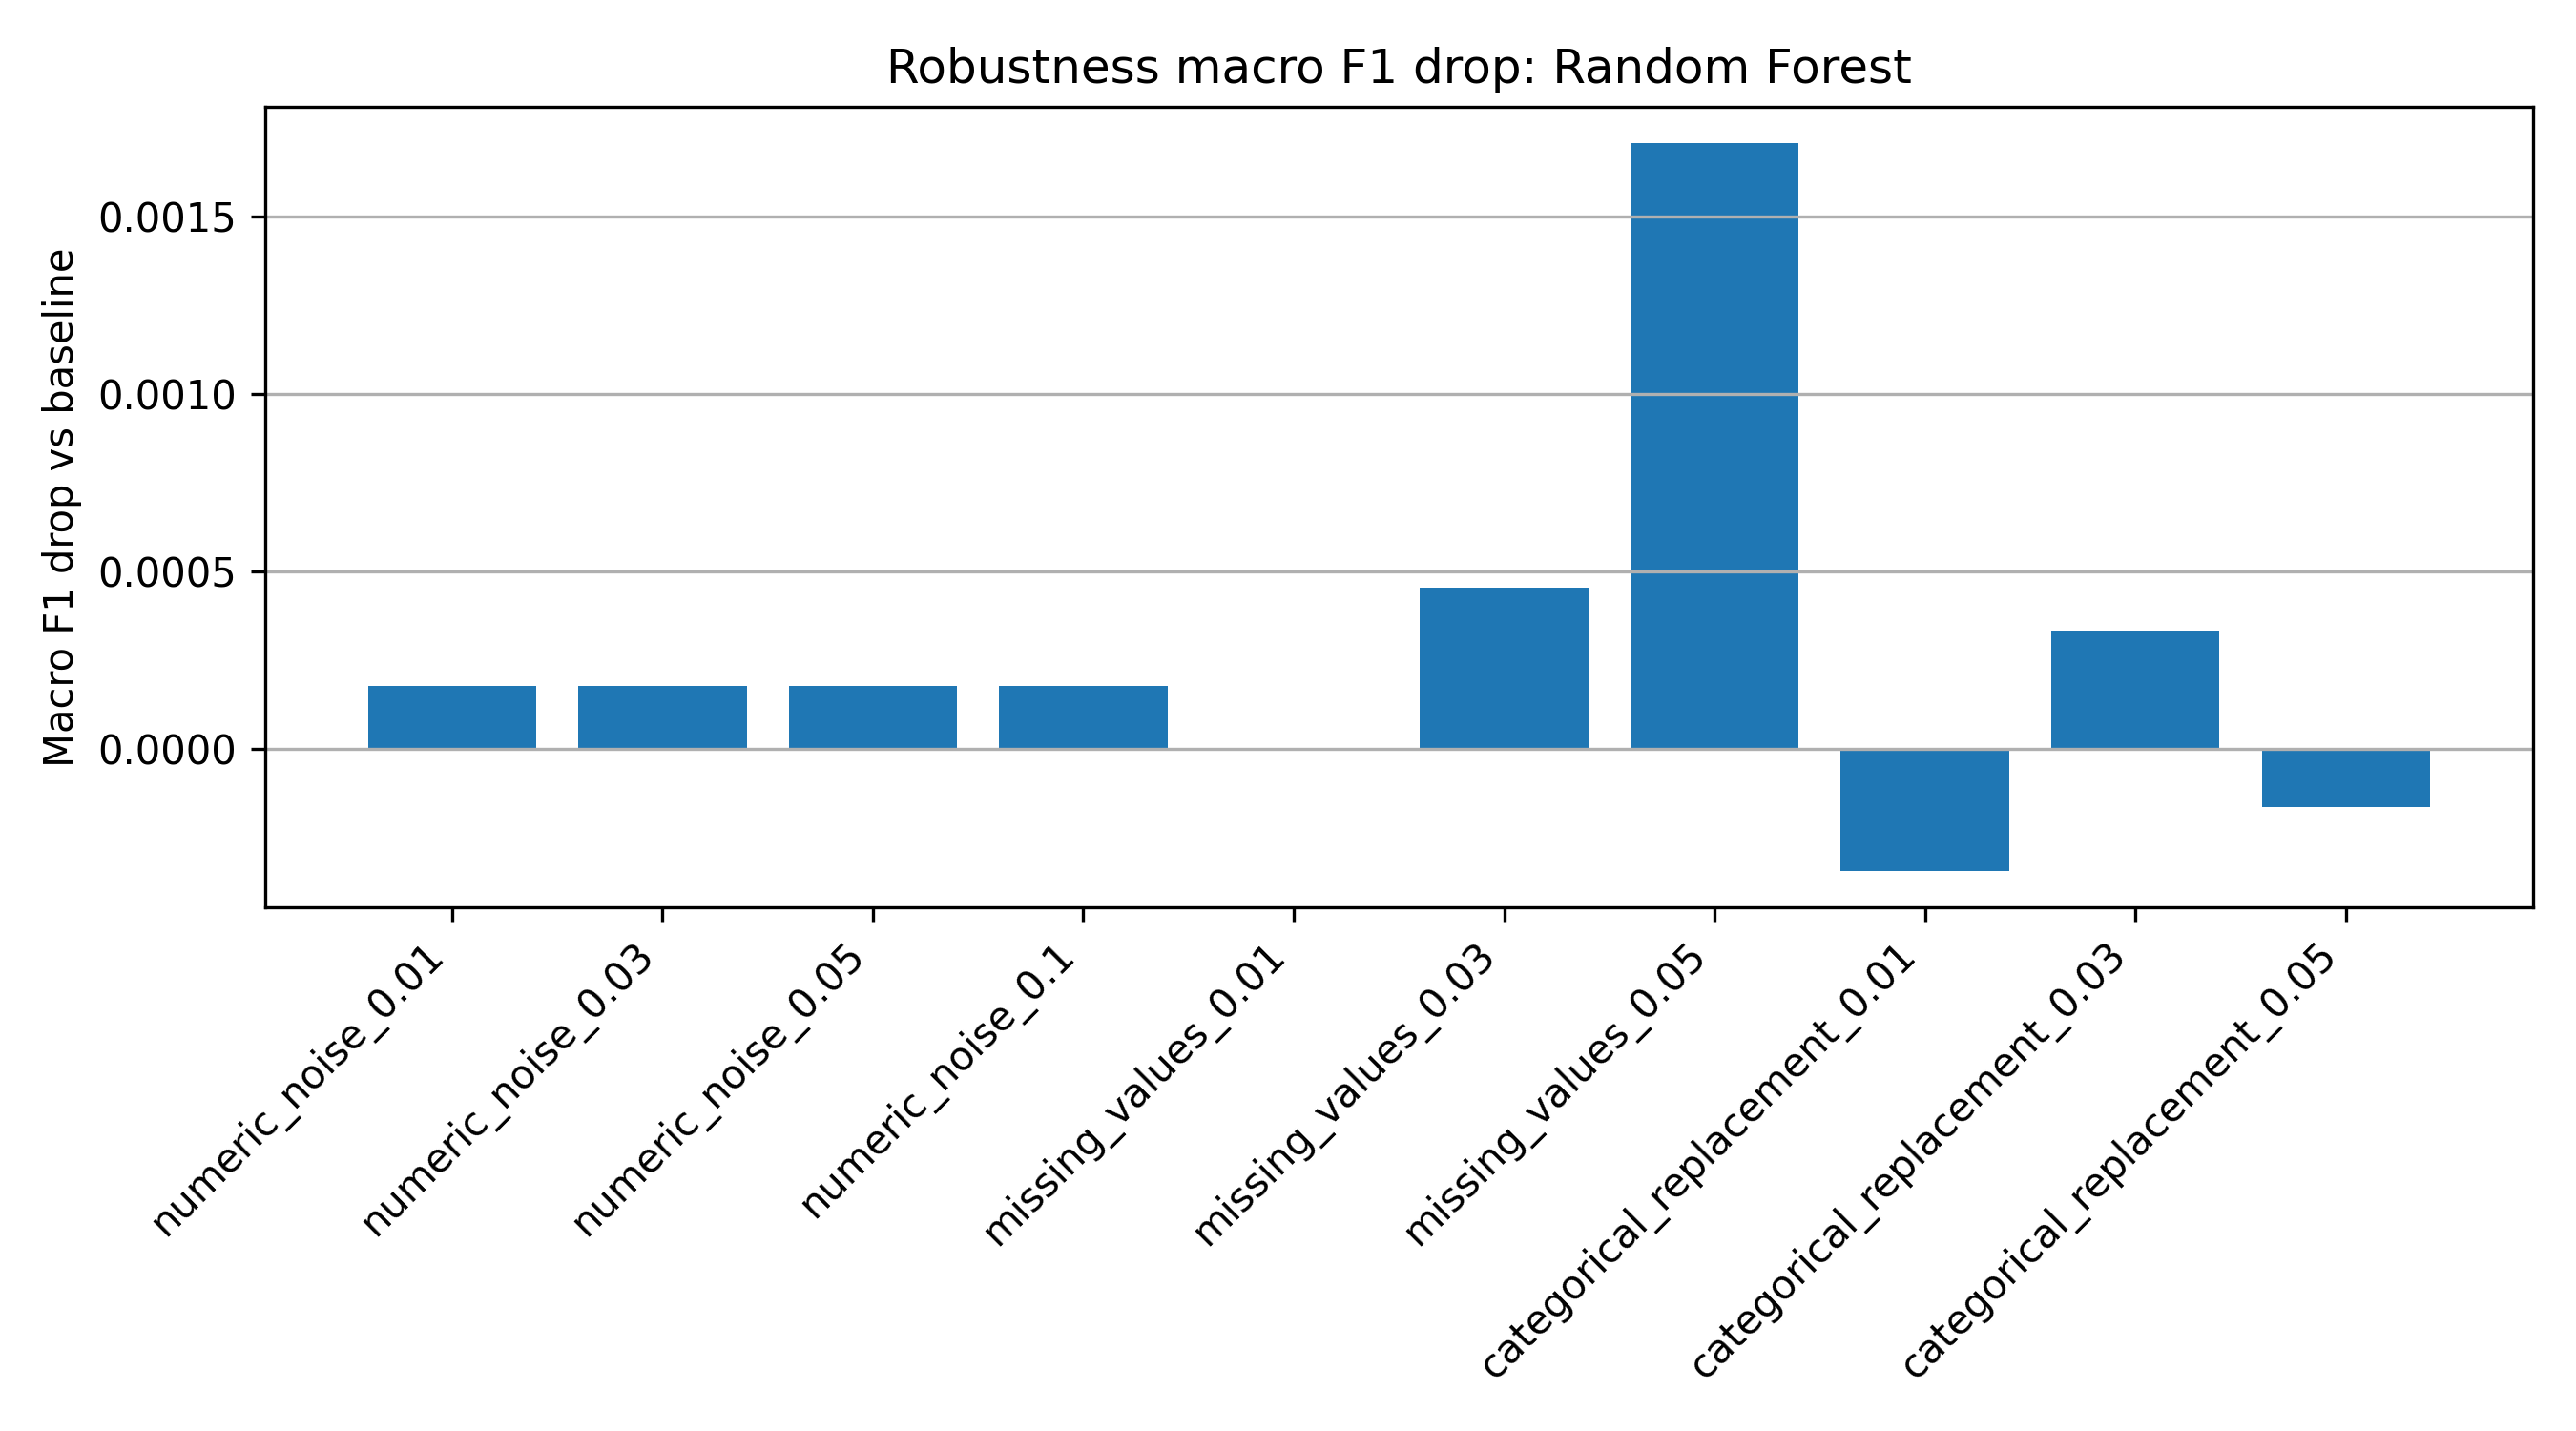
\includegraphics[width=0.82\textwidth]{random_forest_images/random_forest_robustness_f1_drop.png}
\caption{Падение F1-macro при искажениях: Random Forest}
\end{figure}
\begin{figure}[H]
\centering
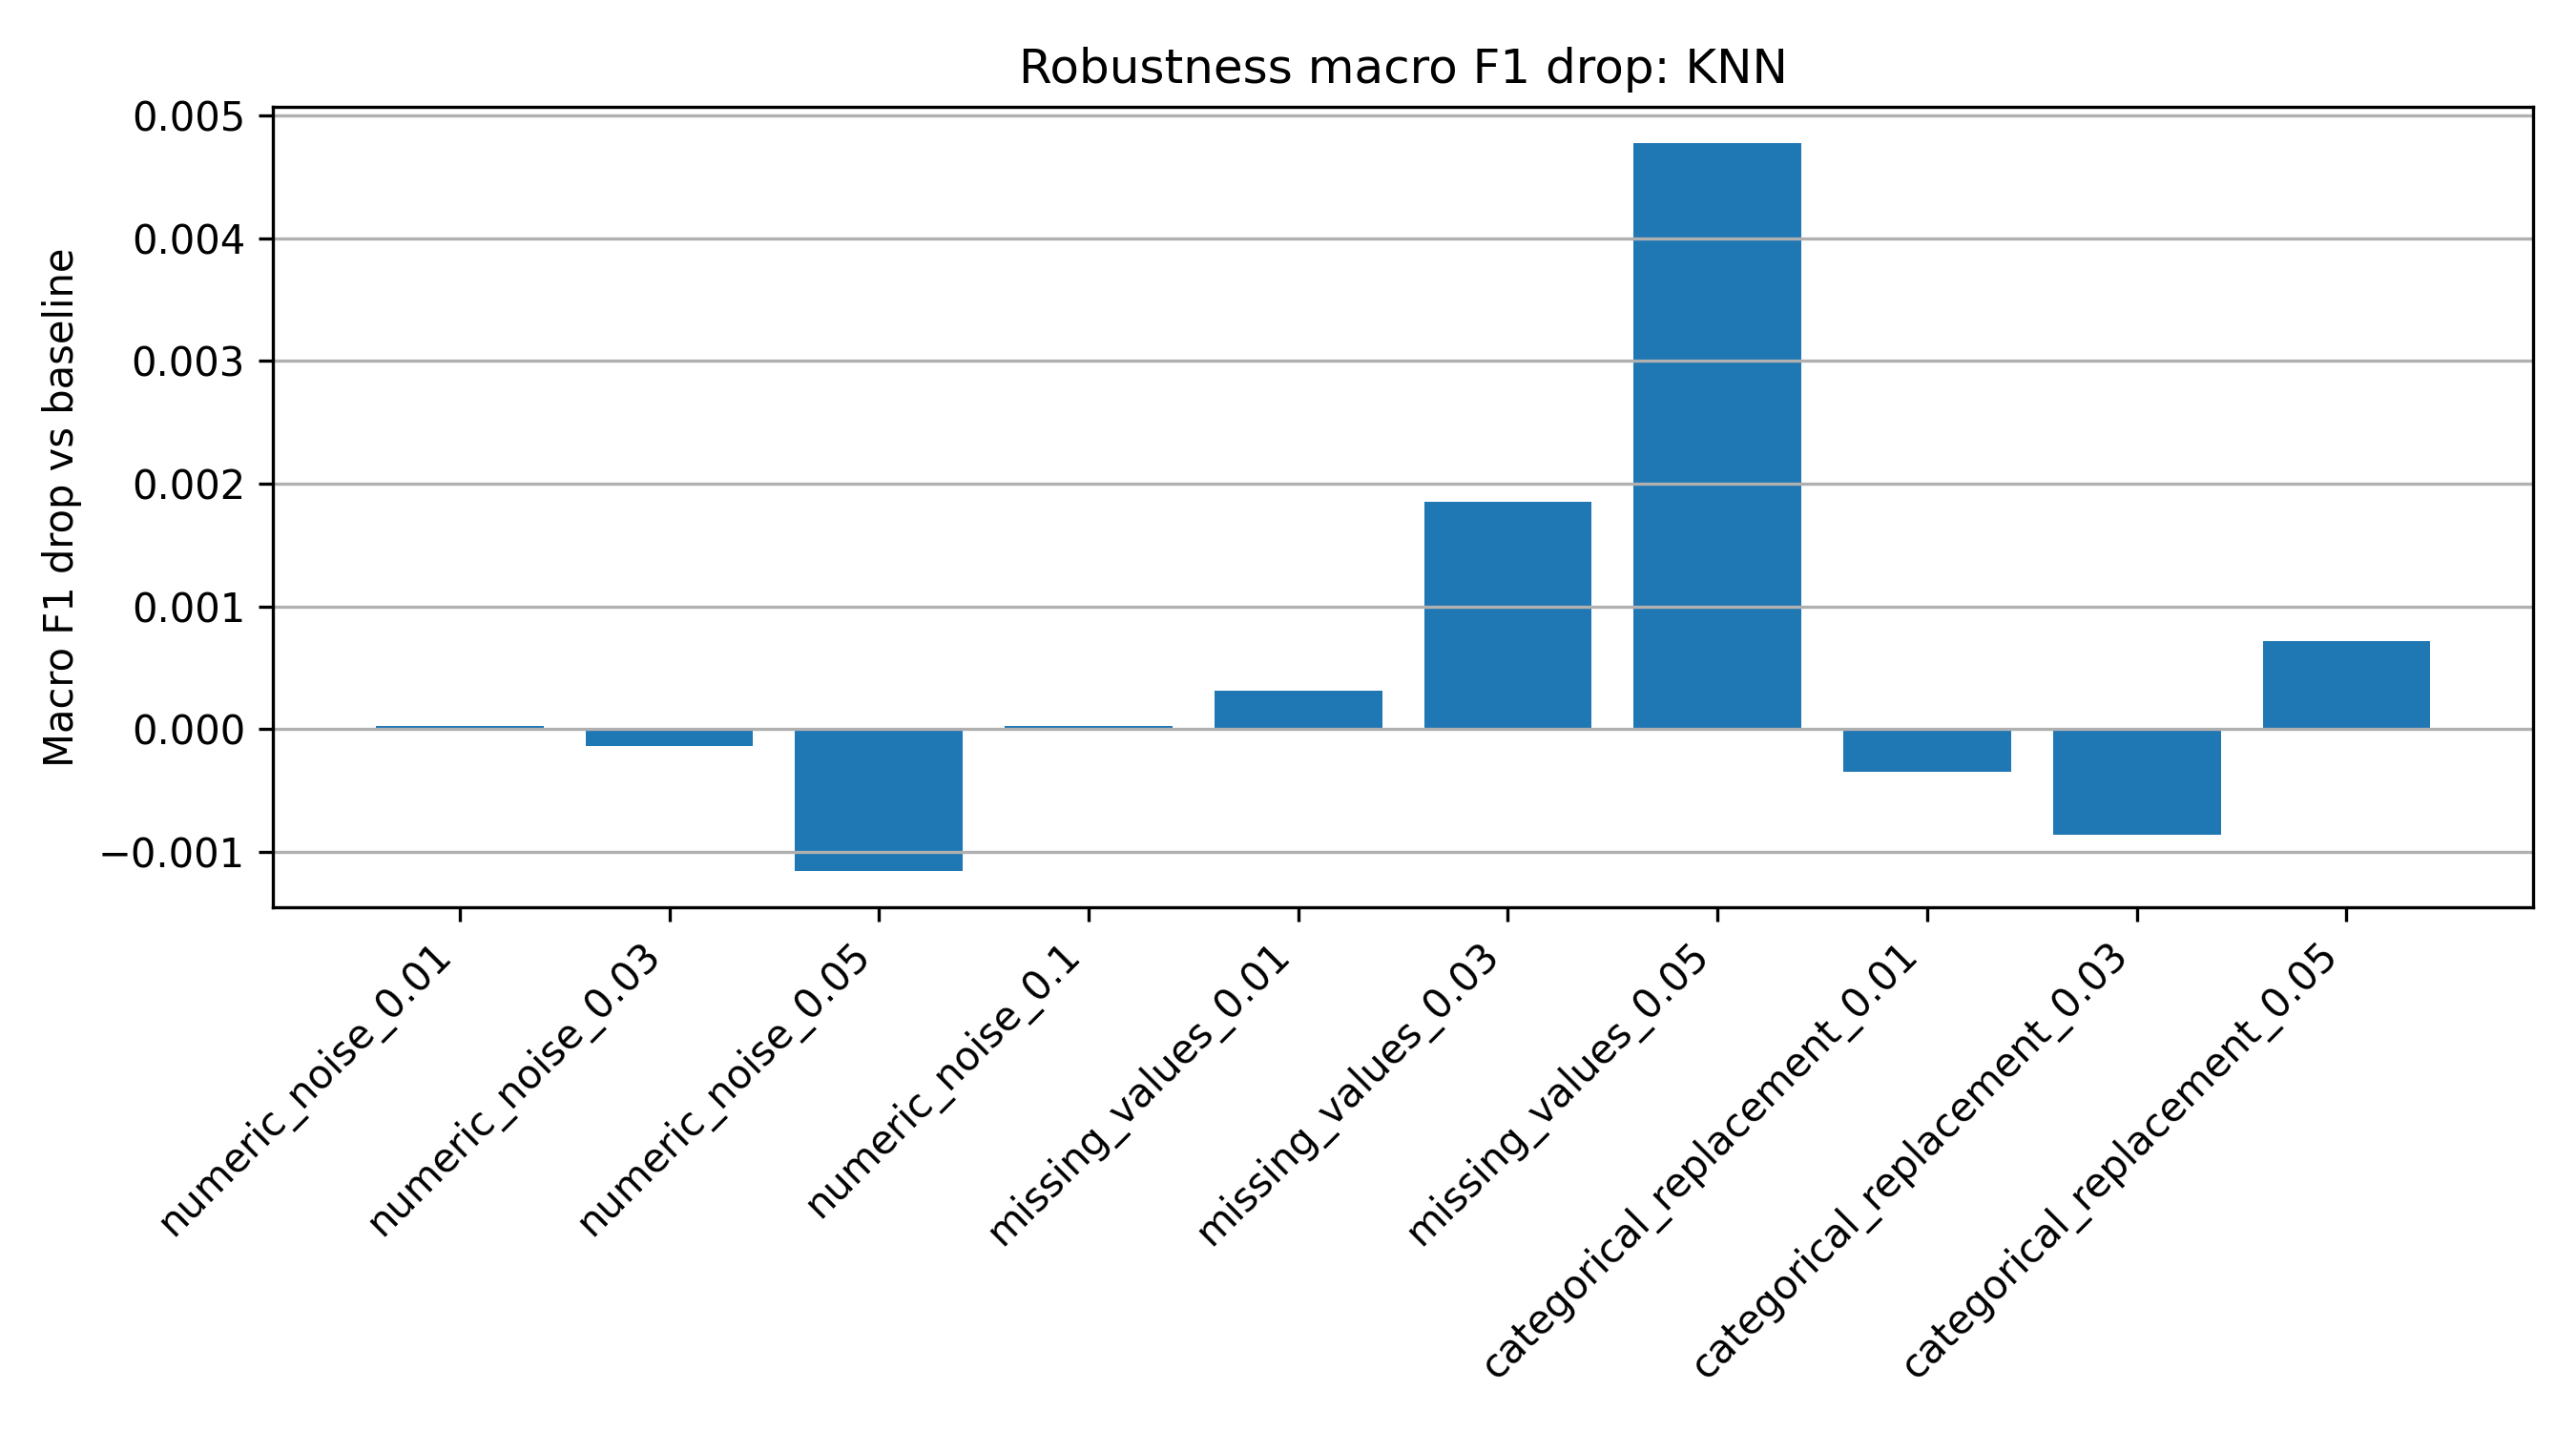
\includegraphics[width=0.82\textwidth]{knn_images/knn_robustness_f1_drop.png}
\caption{Падение F1-macro при искажениях: KNN}
\end{figure}
\begin{figure}[H]
\centering
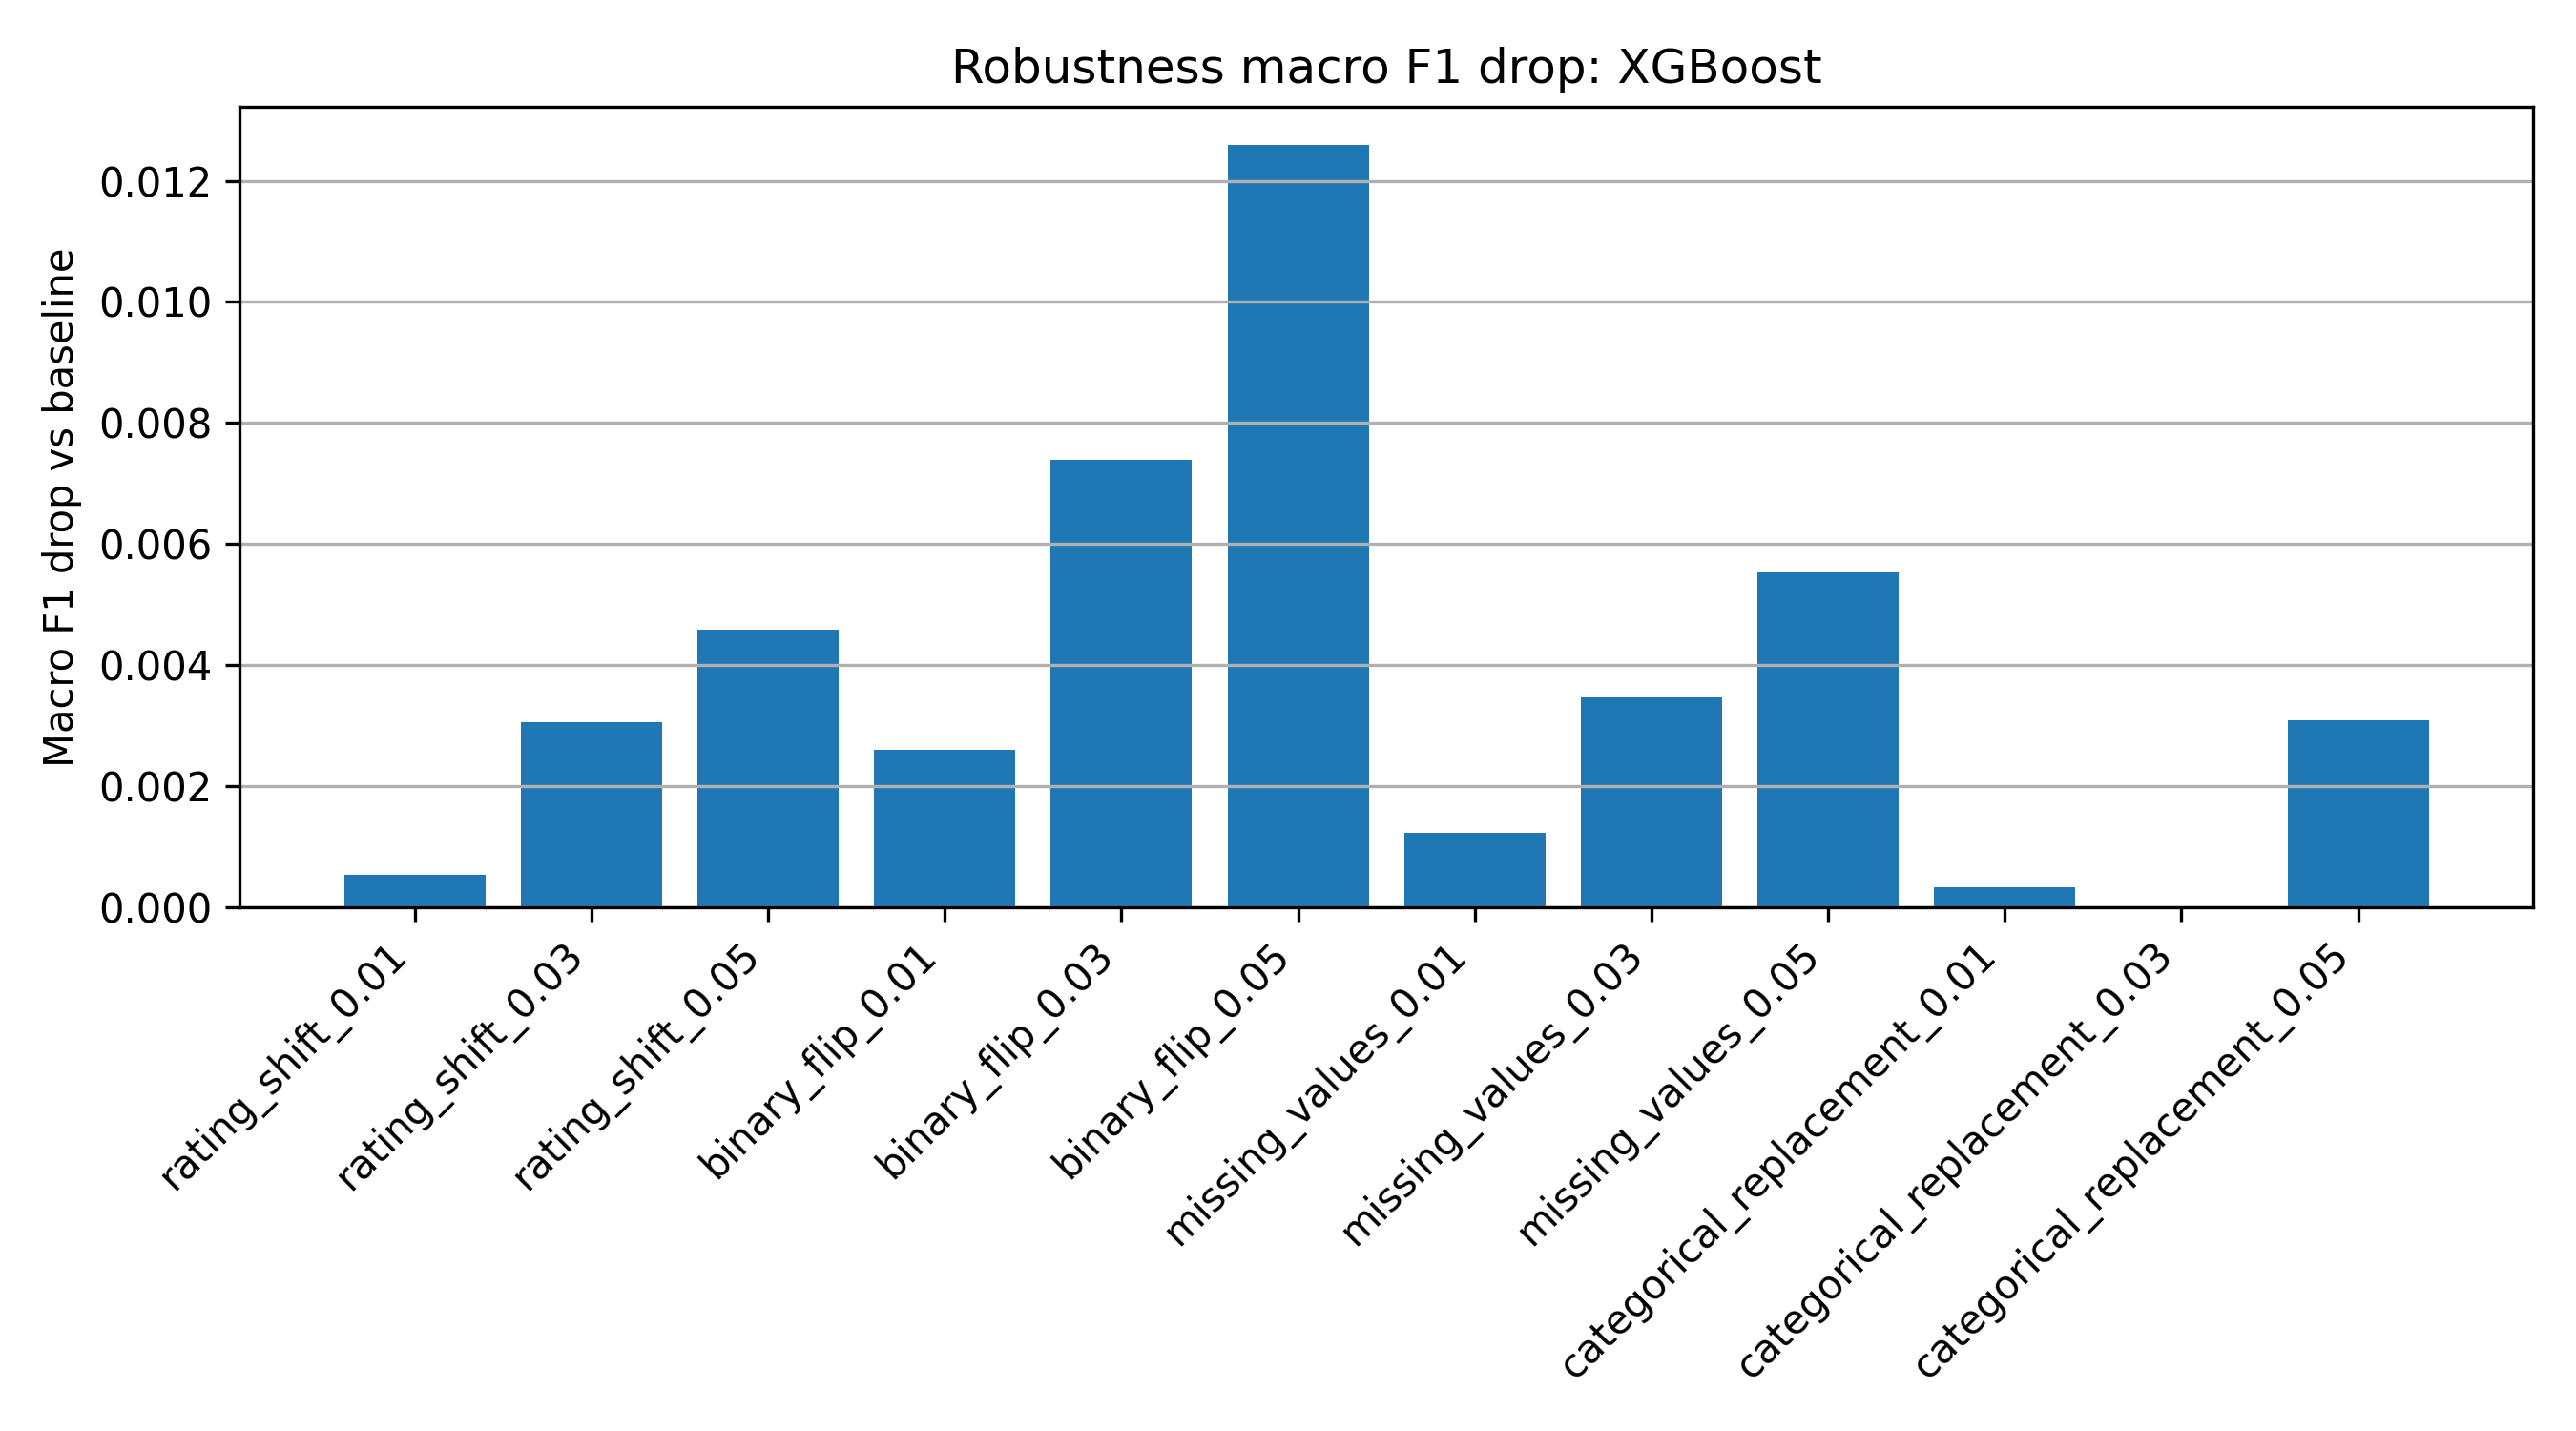
\includegraphics[width=0.82\textwidth]{xgboost_images/xgboost_robustness_f1_drop.png}
\caption{Падение F1-macro при искажениях: XGBoost}
\end{figure}
\begin{figure}[H]
\centering
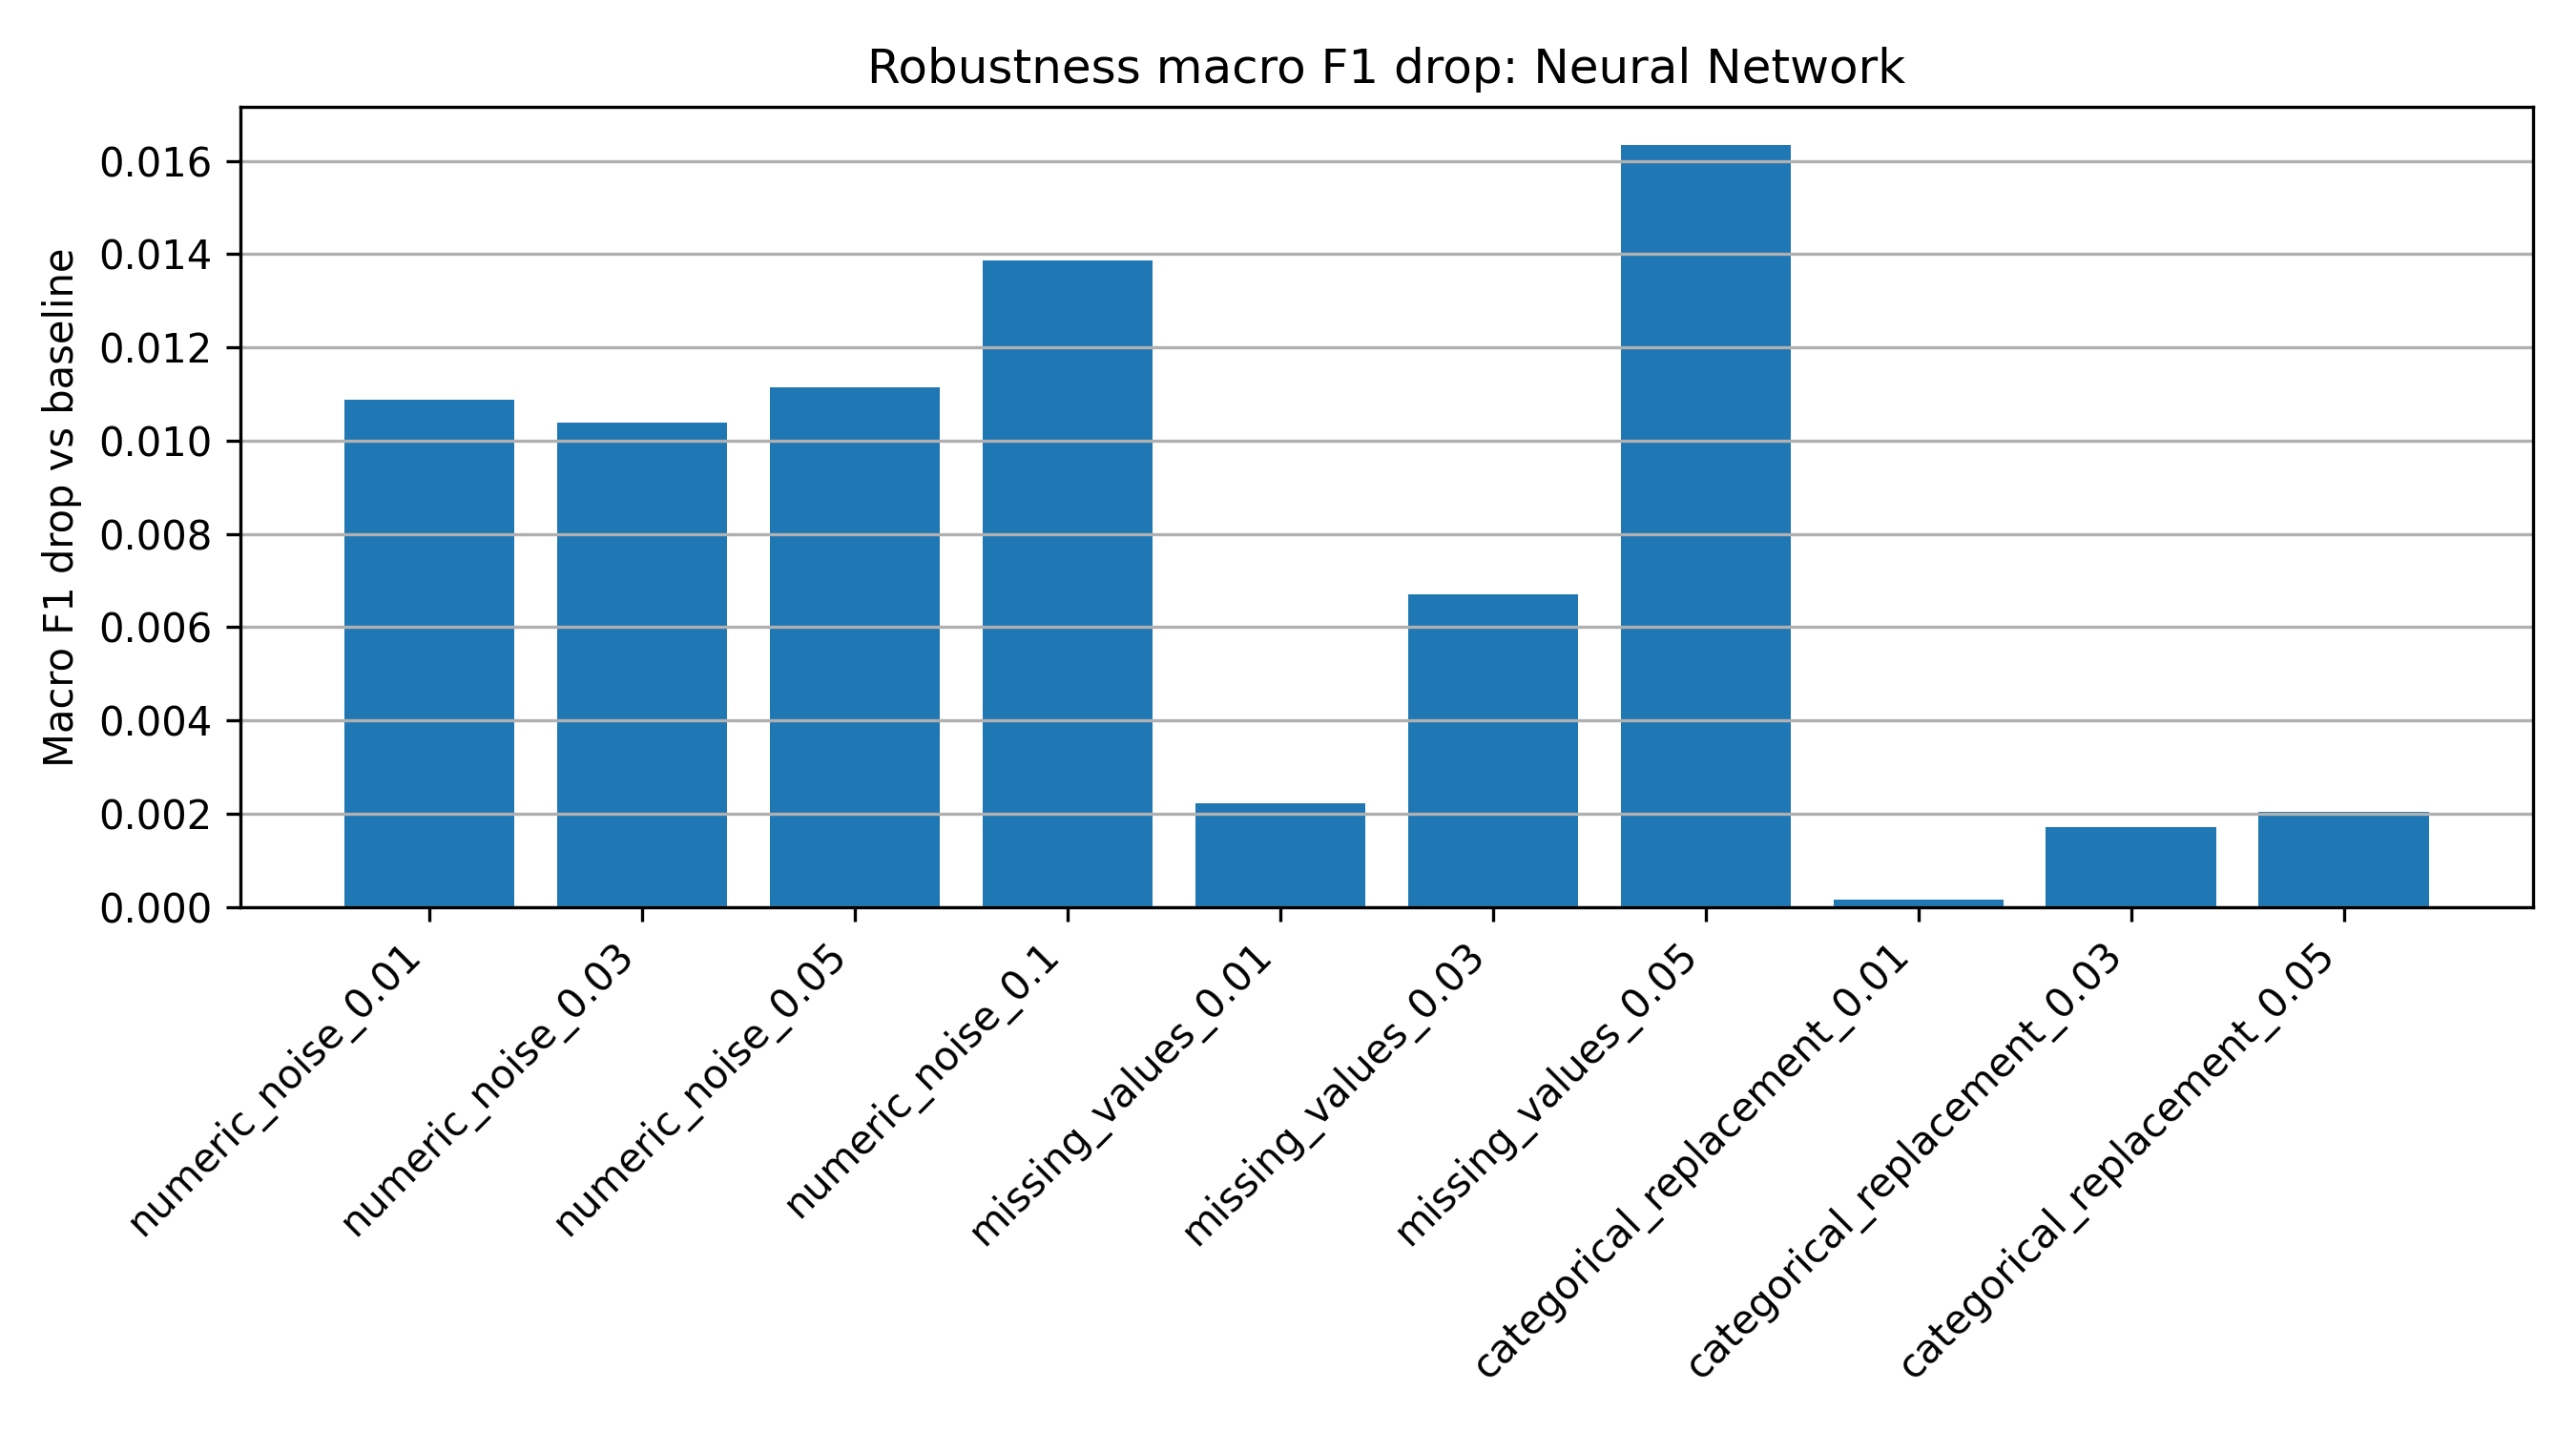
\includegraphics[width=0.82\textwidth]{neural_network_images/neural_network_robustness_f1_drop.png}
\caption{Падение F1-macro при искажениях: Neural Network}
\end{figure}

Проверка устойчивости показывает, насколько качество модели сохраняется при небольших числовых шумах или искажениях категориальных признаков. Наиболее устойчивым в данном эксперименте оказался Random Forest: падение F1-macro в худшем тесте было минимальным. Это ожидаемо для bagging-ансамбля, поскольку усреднение деревьев снижает чувствительность к отдельным искаженным признакам. XGBoost показал лучшее базовое качество, но оказался чувствительнее к числовому шуму, что может быть связано с использованием последовательного бустинга, где деревья уточняют ошибки предыдущих шагов. Более устойчивые модели предпочтительнее для производственного применения, поскольку реальные данные часто содержат ошибки ввода, пропуски и распределительные сдвиги.

\section{Производительность}

\scriptsize
\begin{longtable}{lllllll}
\caption{Сравнение времени обучения и скоринга лучших конфигураций}\label{tab:performance}\\
\toprule
Модель & Тип поиска & CV splits & Mean fit, c & Mean score, c & Score на объект, мс & Mean CV F1 \\
\midrule
\endfirsthead
\toprule
Модель & Тип поиска & CV splits & Mean fit, c & Mean score, c & Score на объект, мс & Mean CV F1 \\
\midrule
\endhead
Logistic Regression & grid & 5 & 1.419 & 0.061 & 0.0059 & 0.810 \\
Decision Tree & grid & 5 & 0.810 & 0.059 & 0.0057 & 0.802 \\
Random Forest & randomized & 5 & 11.482 & 0.312 & 0.0302 & 0.810 \\
KNN & grid & 5 & 0.441 & 1.027 & 0.0991 & 0.800 \\
XGBoost & randomized & 5 & 2.039 & 0.122 & 0.0118 & 0.819 \\
Neural Network & randomized & 5 & 46.768 & 0.241 & 0.0232 & 0.815 \\
\bottomrule
\end{longtable}
\normalsize

В файлах \texttt{models\_performance.csv} сохранены параметры и качество кросс-валидации, а тайминги лучших конфигураций берутся из файлов \texttt{*\_cv\_search\_results.csv}, где \texttt{mean\_fit\_time} отражает среднее время обучения на одном CV-fold, а \texttt{mean\_score\_time} --- среднее время получения предсказаний и расчета scorer на validation-fold. Значение ``Score на объект'' рассчитано как \texttt{mean\_score\_time}, деленное на примерный размер validation-fold.

Самой быстрой по обучению среди рассмотренных моделей оказалась KNN, однако это связано с ленивой природой метода: модель почти не обучает параметры, но переносит основную вычислительную нагрузку на этап предсказания. Поэтому KNN имеет худшее среднее время скоринга на объект. Decision Tree и Logistic Regression дают быстрые обучение и скоринг, но уступают лучшим моделям по качеству. XGBoost показывает лучший компромисс: он существенно качественнее простых моделей, быстрее Random Forest и значительно быстрее нейронной сети на этапе обучения. Neural Network оказалась самой дорогой по времени обучения из-за многократных эпох оптимизации, при этом по качеству она не превзошла XGBoost.

\section{Перестановочная важность признаков}

\scriptsize
\begin{longtable}{lllll}
\caption{Топ-5 признаков по permutation importance для каждой модели}\label{tab:permutation_importance}\\
\toprule
Модель & Ранг & Признак & Importance mean & Importance std \\
\midrule
\endfirsthead
\toprule
Модель & Ранг & Признак & Importance mean & Importance std \\
\midrule
\endhead
Logistic Regression & 1 & location\_and\_movement & 0.0312 & 0.0021 \\
Logistic Regression & 2 & curbside\_dropoff\_ease & 0.0159 & 0.0020 \\
Logistic Regression & 3 & boarding\_lounge\_comfort & 0.0074 & 0.0018 \\
Logistic Regression & 4 & overall\_airport\_cleanliness & 0.0073 & 0.0008 \\
Logistic Regression & 5 & ticket\_purchase\_process & 0.0039 & 0.0008 \\
Decision Tree & 1 & location\_and\_movement & 0.1239 & 0.0045 \\
Decision Tree & 2 & overall\_airport\_cleanliness & 0.0412 & 0.0035 \\
Decision Tree & 3 & boarding\_lounge\_comfort & 0.0174 & 0.0005 \\
Decision Tree & 4 & thermal\_comfort & 0.0142 & 0.0018 \\
Decision Tree & 5 & food\_beverage\_quality\_variety & 0.0060 & 0.0007 \\
Random Forest & 1 & location\_and\_movement & 0.0289 & 0.0025 \\
Random Forest & 2 & overall\_airport\_cleanliness & 0.0253 & 0.0010 \\
Random Forest & 3 & boarding\_lounge\_comfort & 0.0060 & 0.0019 \\
Random Forest & 4 & flight\_information\_display\_availability & 0.0027 & 0.0004 \\
Random Forest & 5 & restrooms & 0.0019 & 0.0011 \\
KNN & 1 & location\_and\_movement & 0.0054 & 0.0024 \\
KNN & 2 & overall\_airport\_cleanliness & 0.0033 & 0.0003 \\
KNN & 3 & thermal\_comfort & 0.0028 & 0.0009 \\
KNN & 4 & seat\_availability & 0.0028 & 0.0004 \\
KNN & 5 & ticket\_purchase\_process & 0.0023 & 0.0015 \\
XGBoost & 1 & location\_and\_movement & 0.0409 & 0.0034 \\
XGBoost & 2 & overall\_airport\_cleanliness & 0.0242 & 0.0021 \\
XGBoost & 3 & boarding\_lounge\_comfort & 0.0084 & 0.0018 \\
XGBoost & 4 & power\_outlet\_availability & 0.0075 & 0.0013 \\
XGBoost & 5 & security\_screening\_process & 0.0045 & 0.0014 \\
Neural Network & 1 & location\_and\_movement & 0.0485 & 0.0016 \\
Neural Network & 2 & curbside\_dropoff\_ease & 0.0239 & 0.0033 \\
Neural Network & 3 & overall\_airport\_cleanliness & 0.0180 & 0.0023 \\
Neural Network & 4 & boarding\_lounge\_comfort & 0.0122 & 0.0025 \\
Neural Network & 5 & thermal\_comfort & 0.0062 & 0.0007 \\
\bottomrule
\end{longtable}
\normalsize
\begin{figure}[H]
\centering
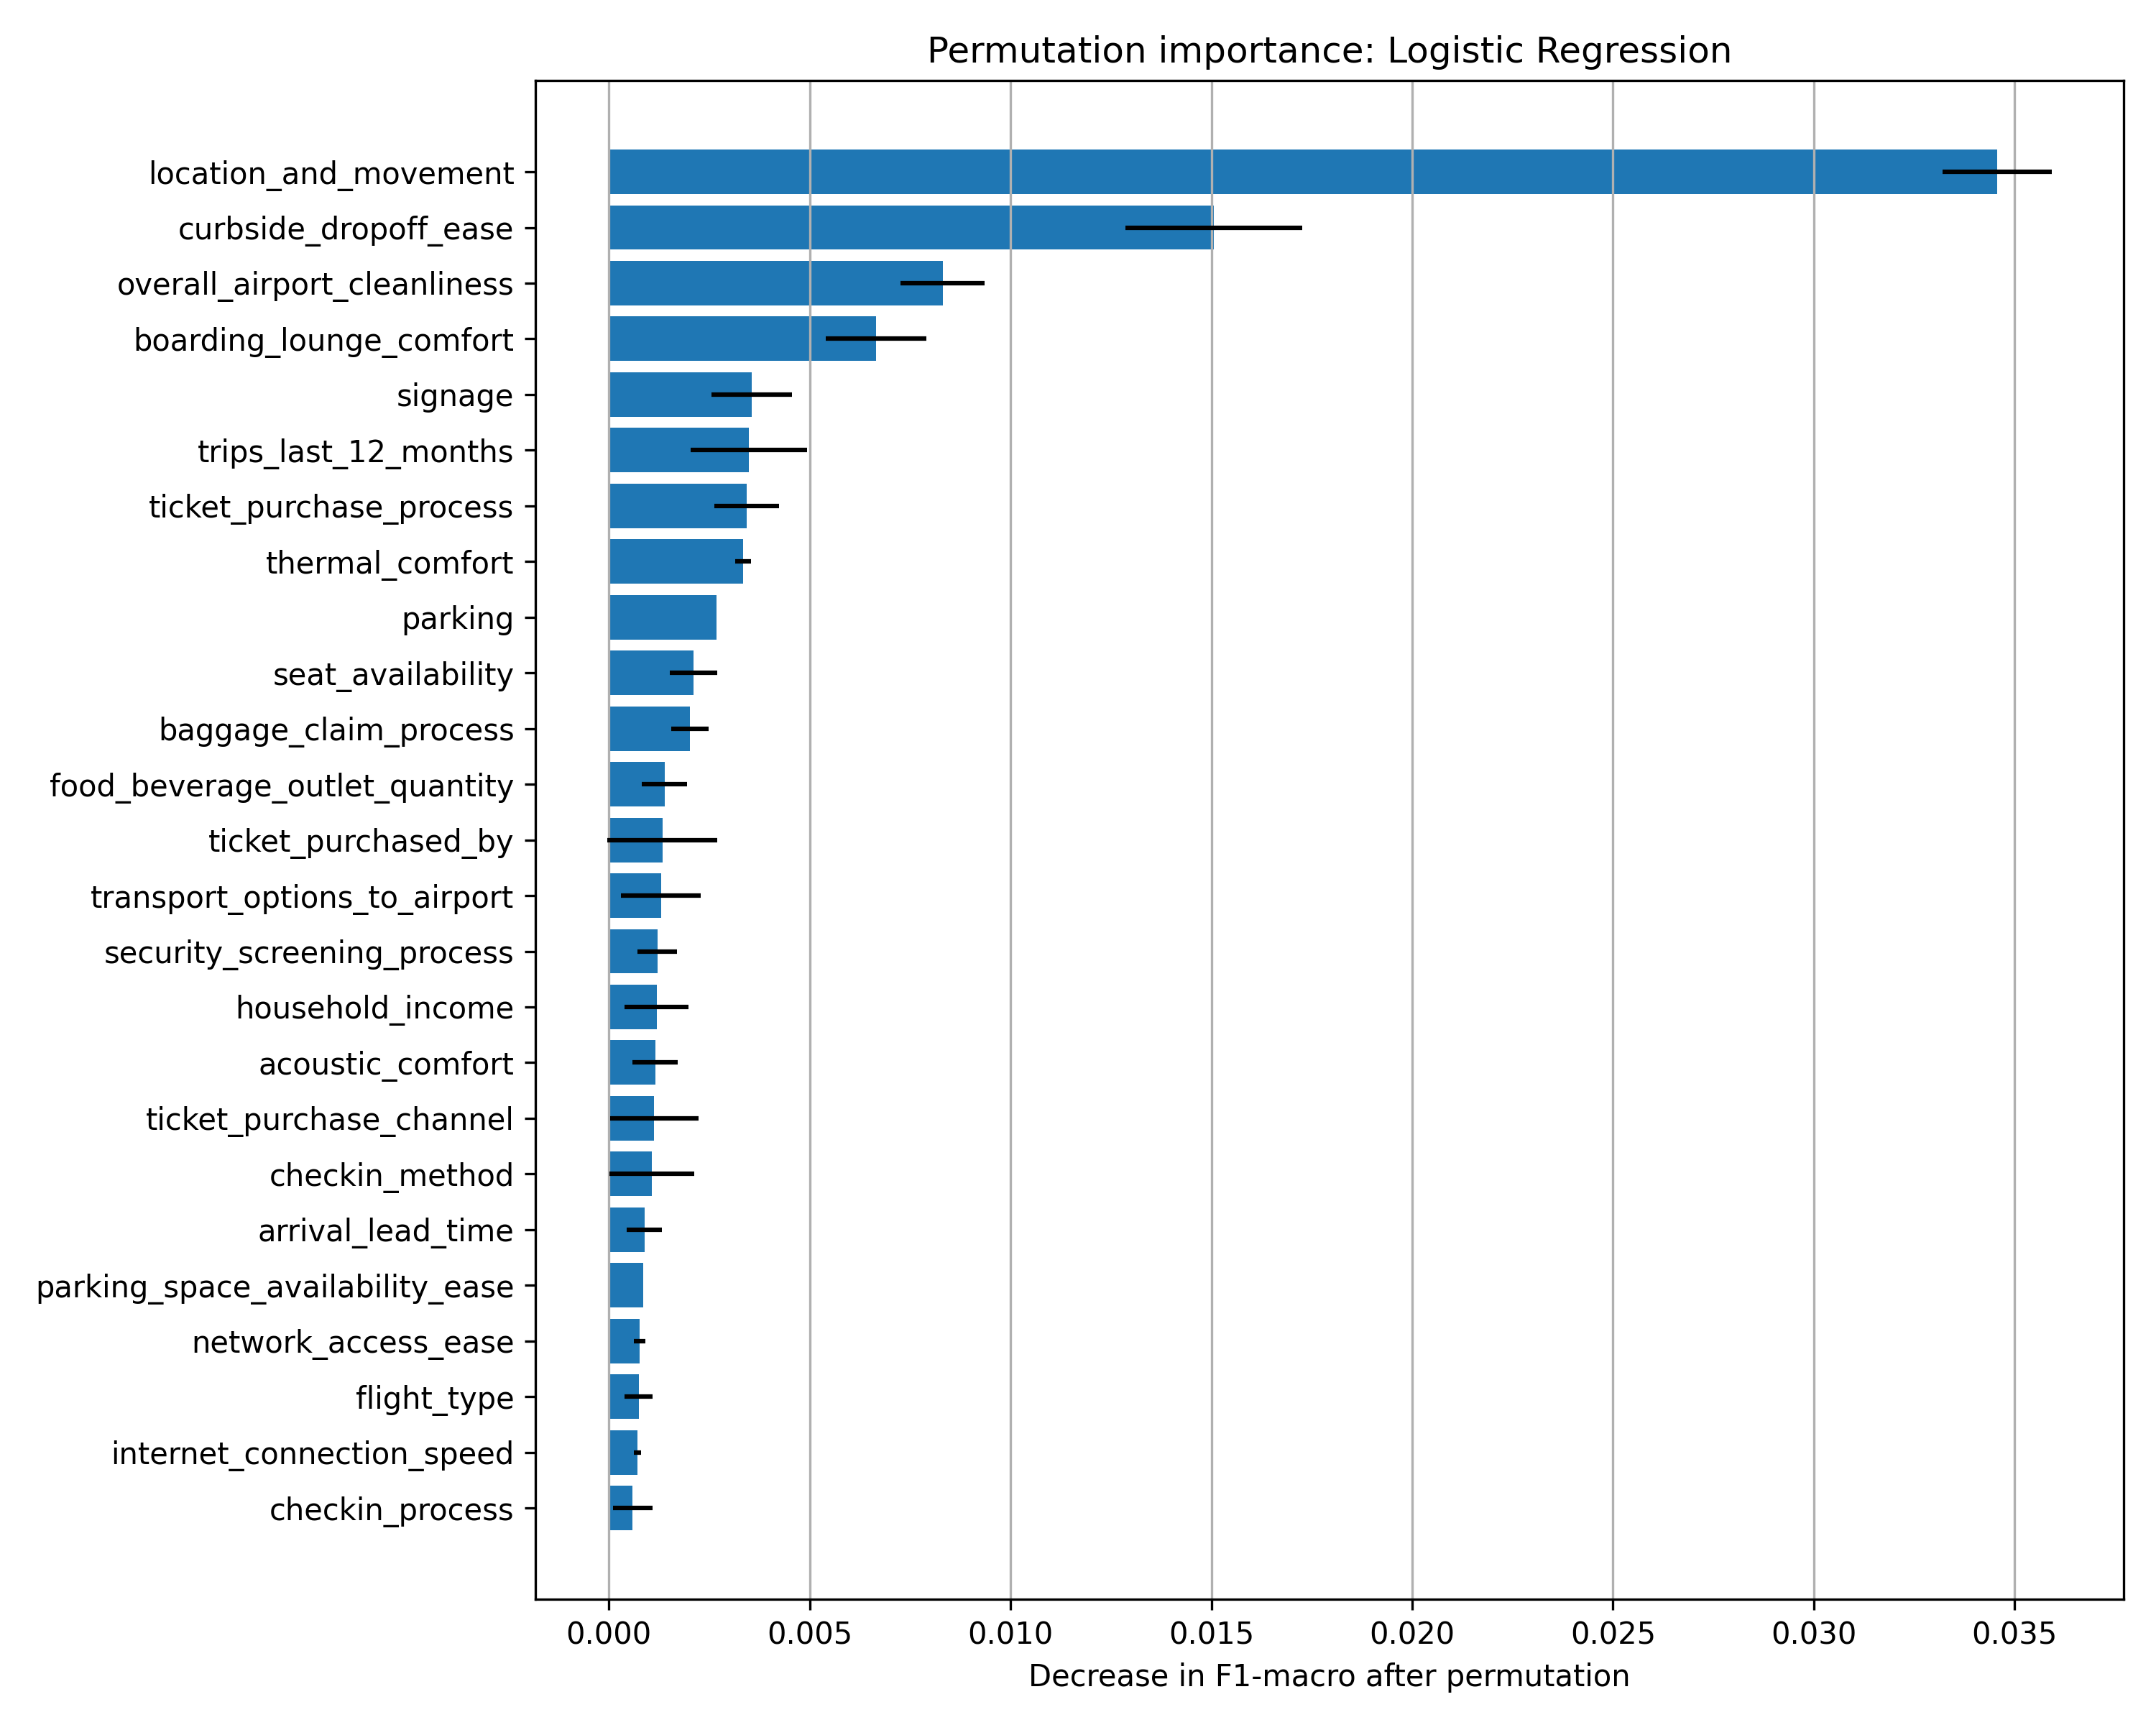
\includegraphics[width=0.82\textwidth]{logistic_regression_images/logistic_regression_permutation_importance.png}
\caption{Permutation importance: Logistic Regression}
\end{figure}
\begin{figure}[H]
\centering
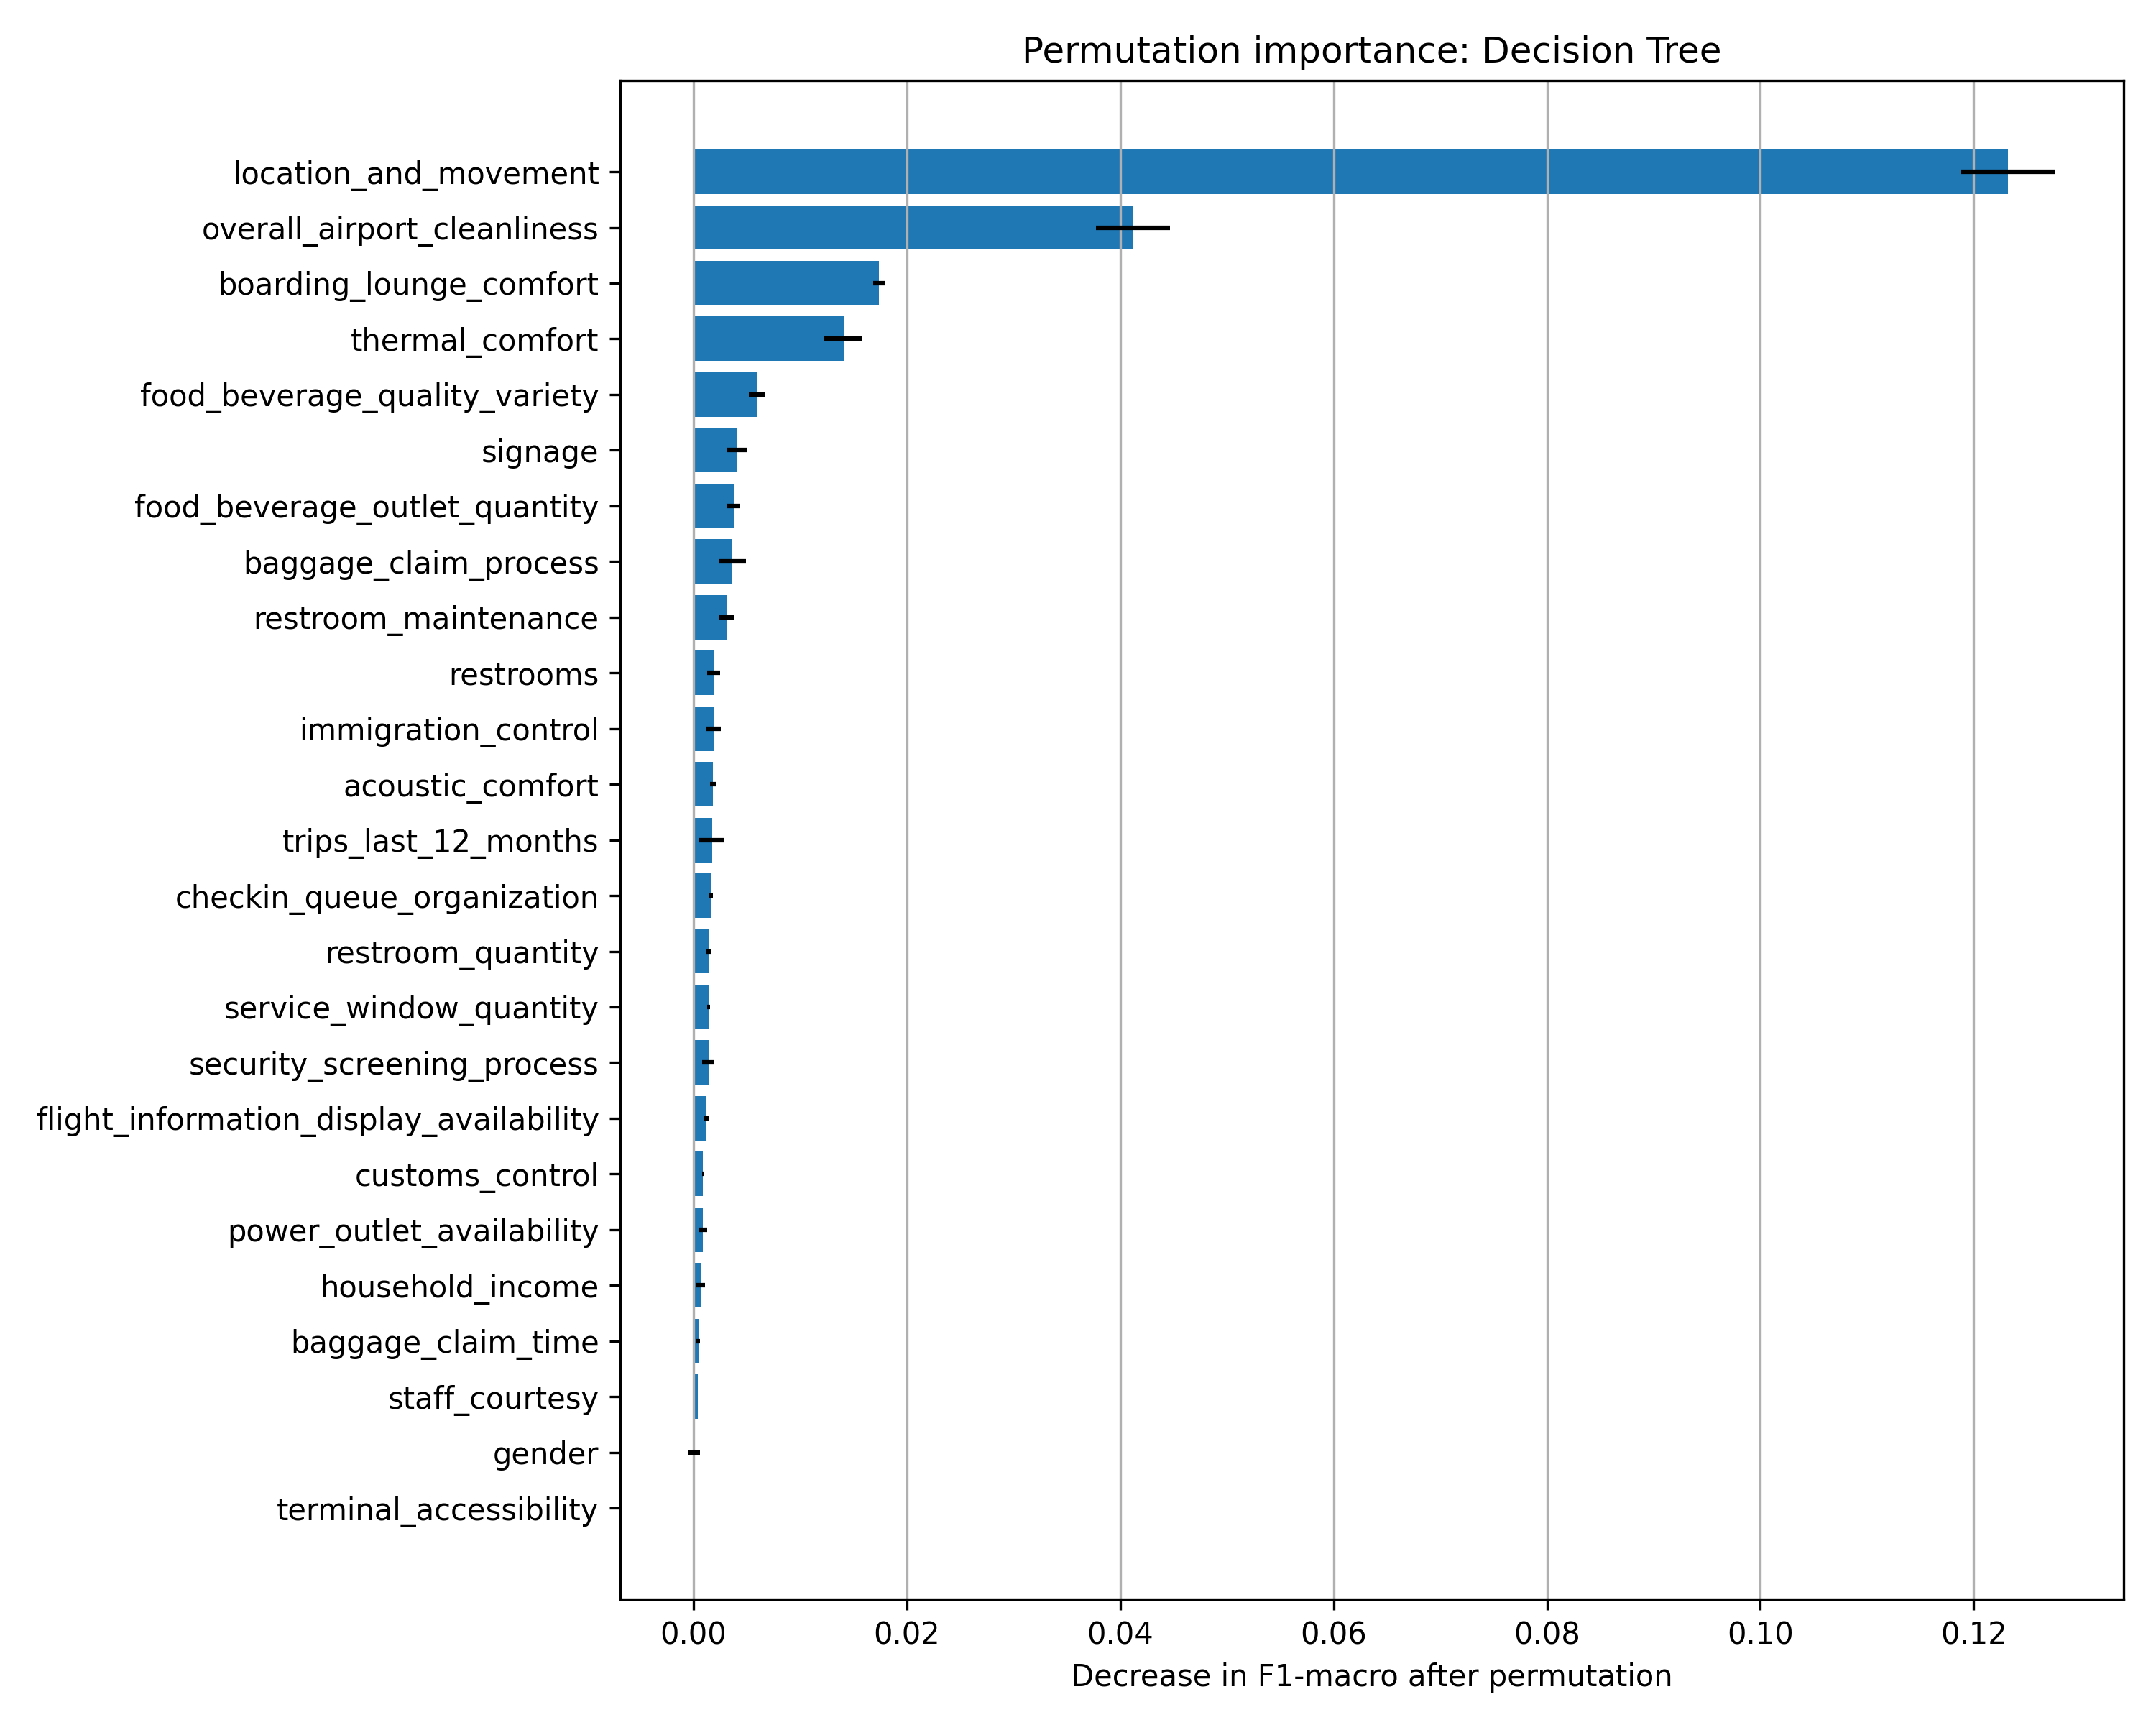
\includegraphics[width=0.82\textwidth]{decision_tree_images/decision_tree_permutation_importance.png}
\caption{Permutation importance: Decision Tree}
\end{figure}
\begin{figure}[H]
\centering
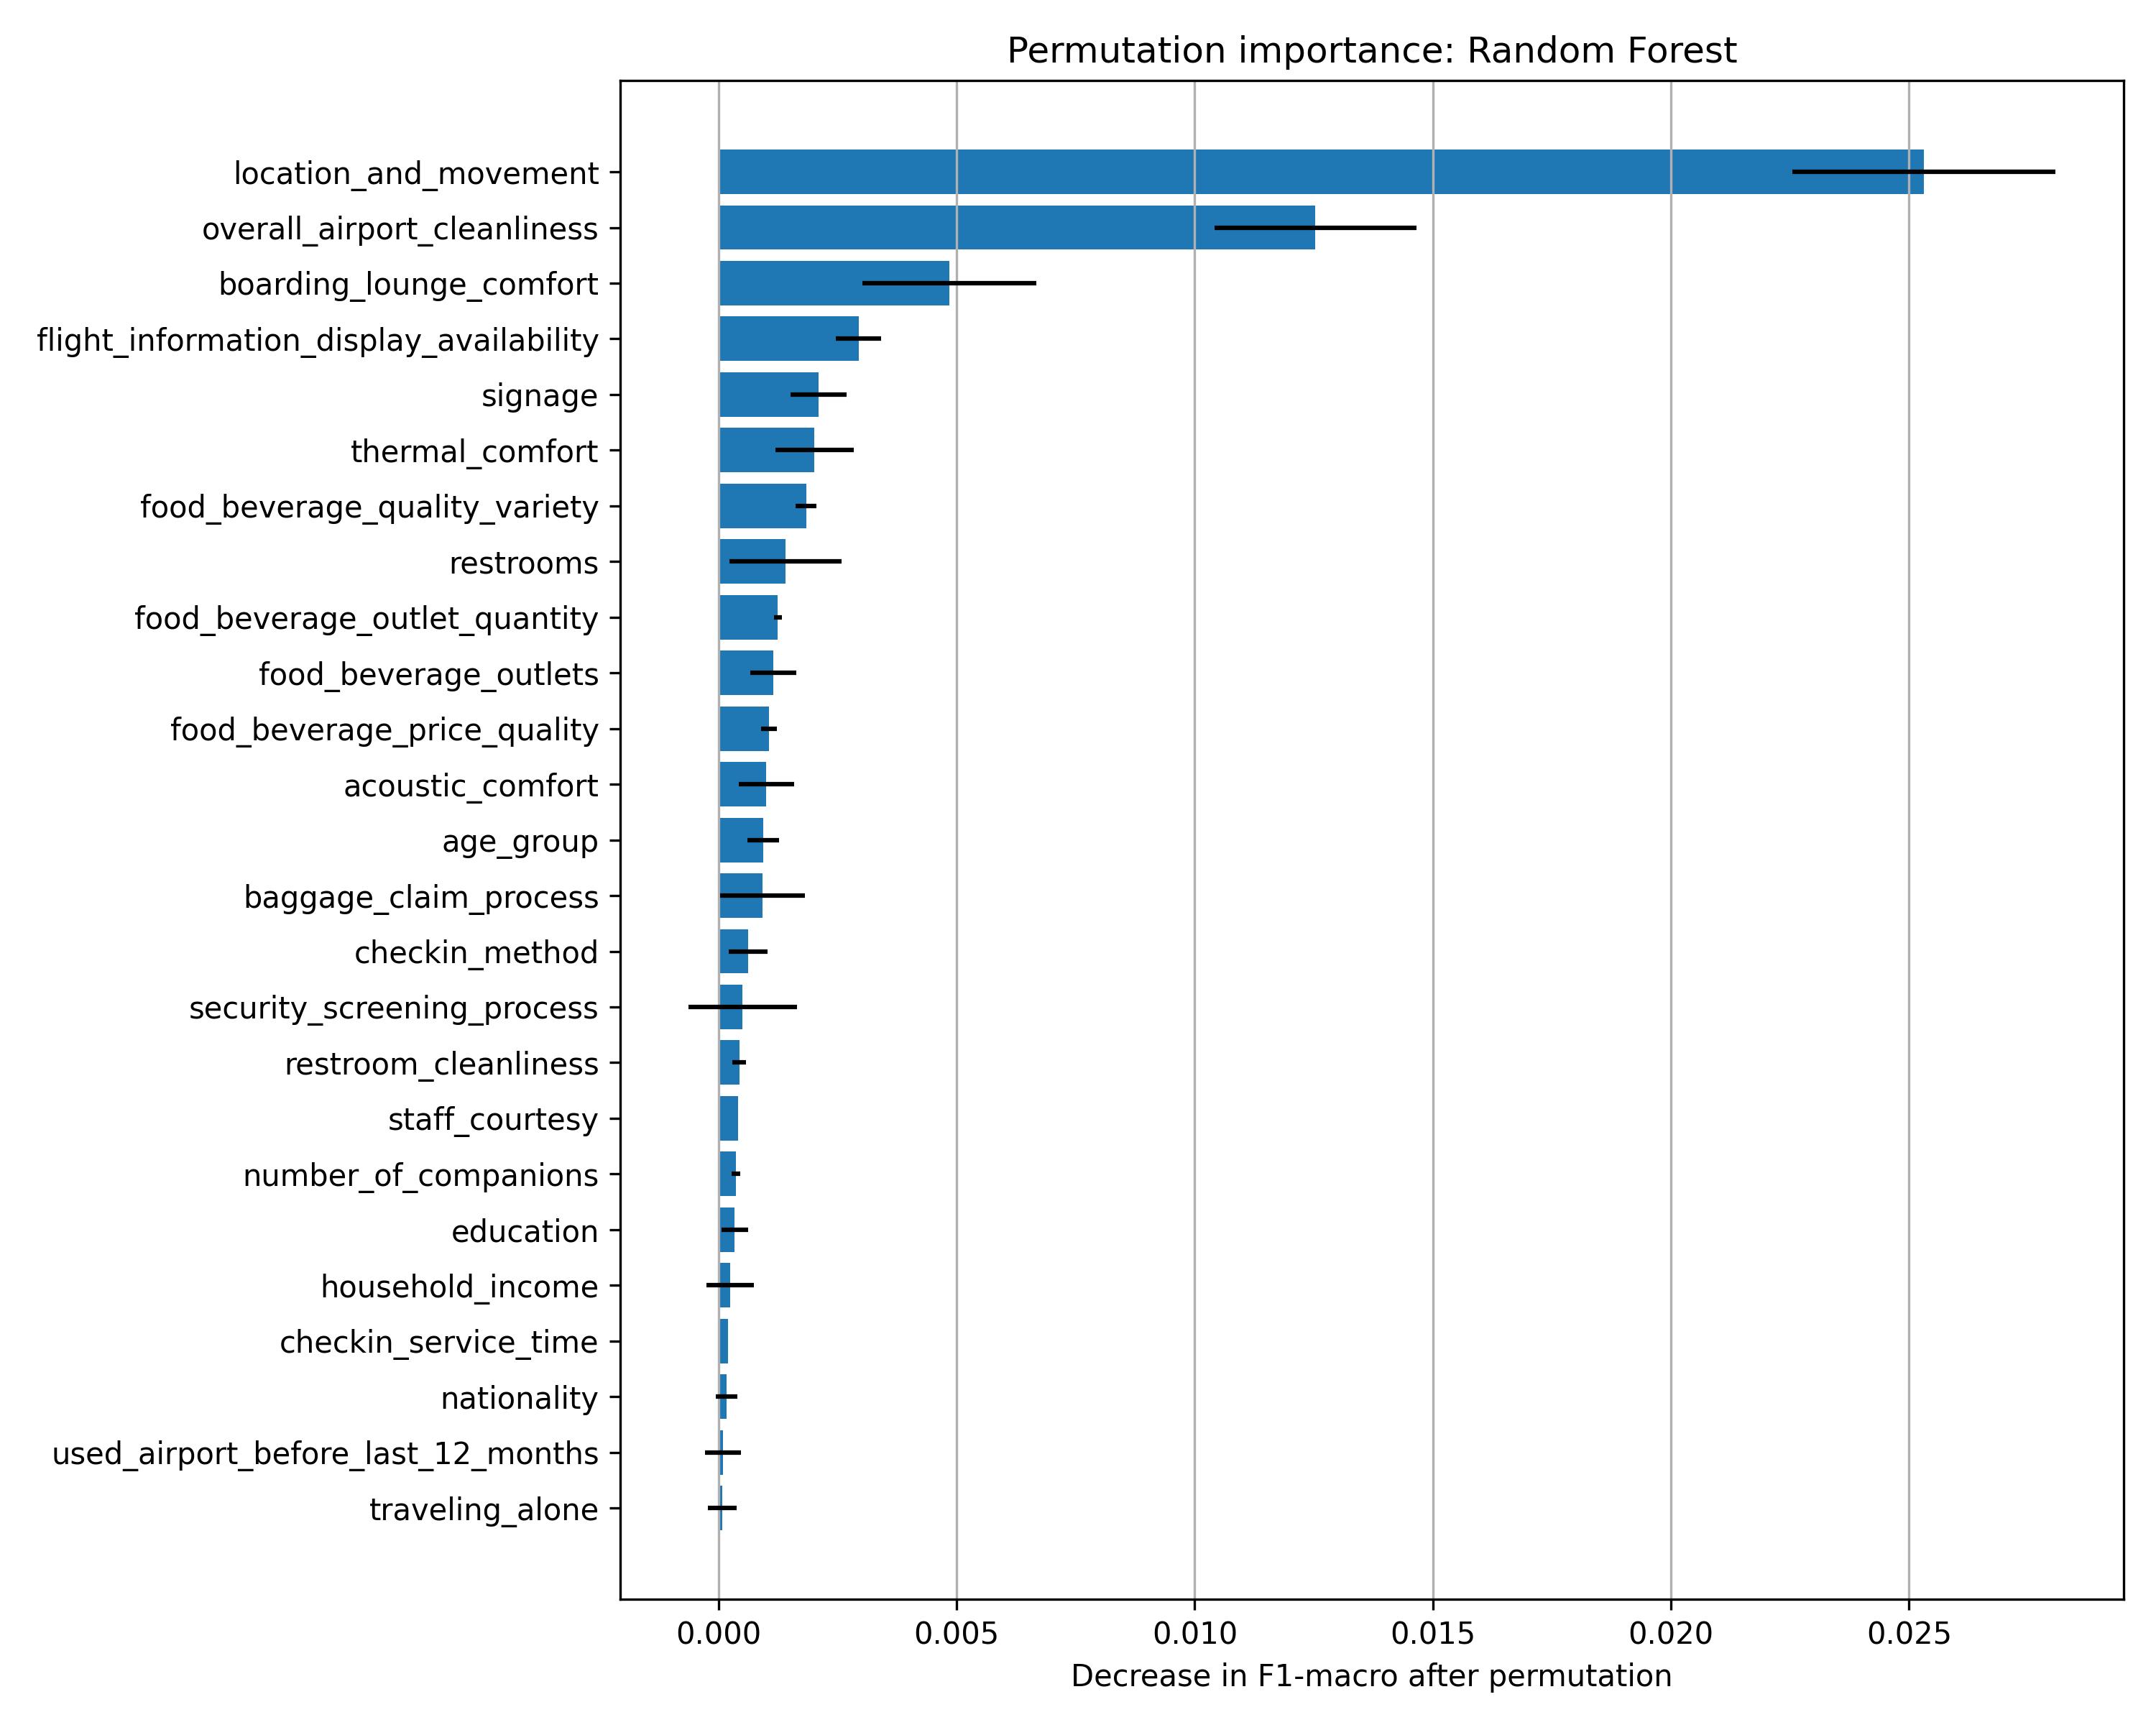
\includegraphics[width=0.82\textwidth]{random_forest_images/random_forest_permutation_importance.png}
\caption{Permutation importance: Random Forest}
\end{figure}
\begin{figure}[H]
\centering
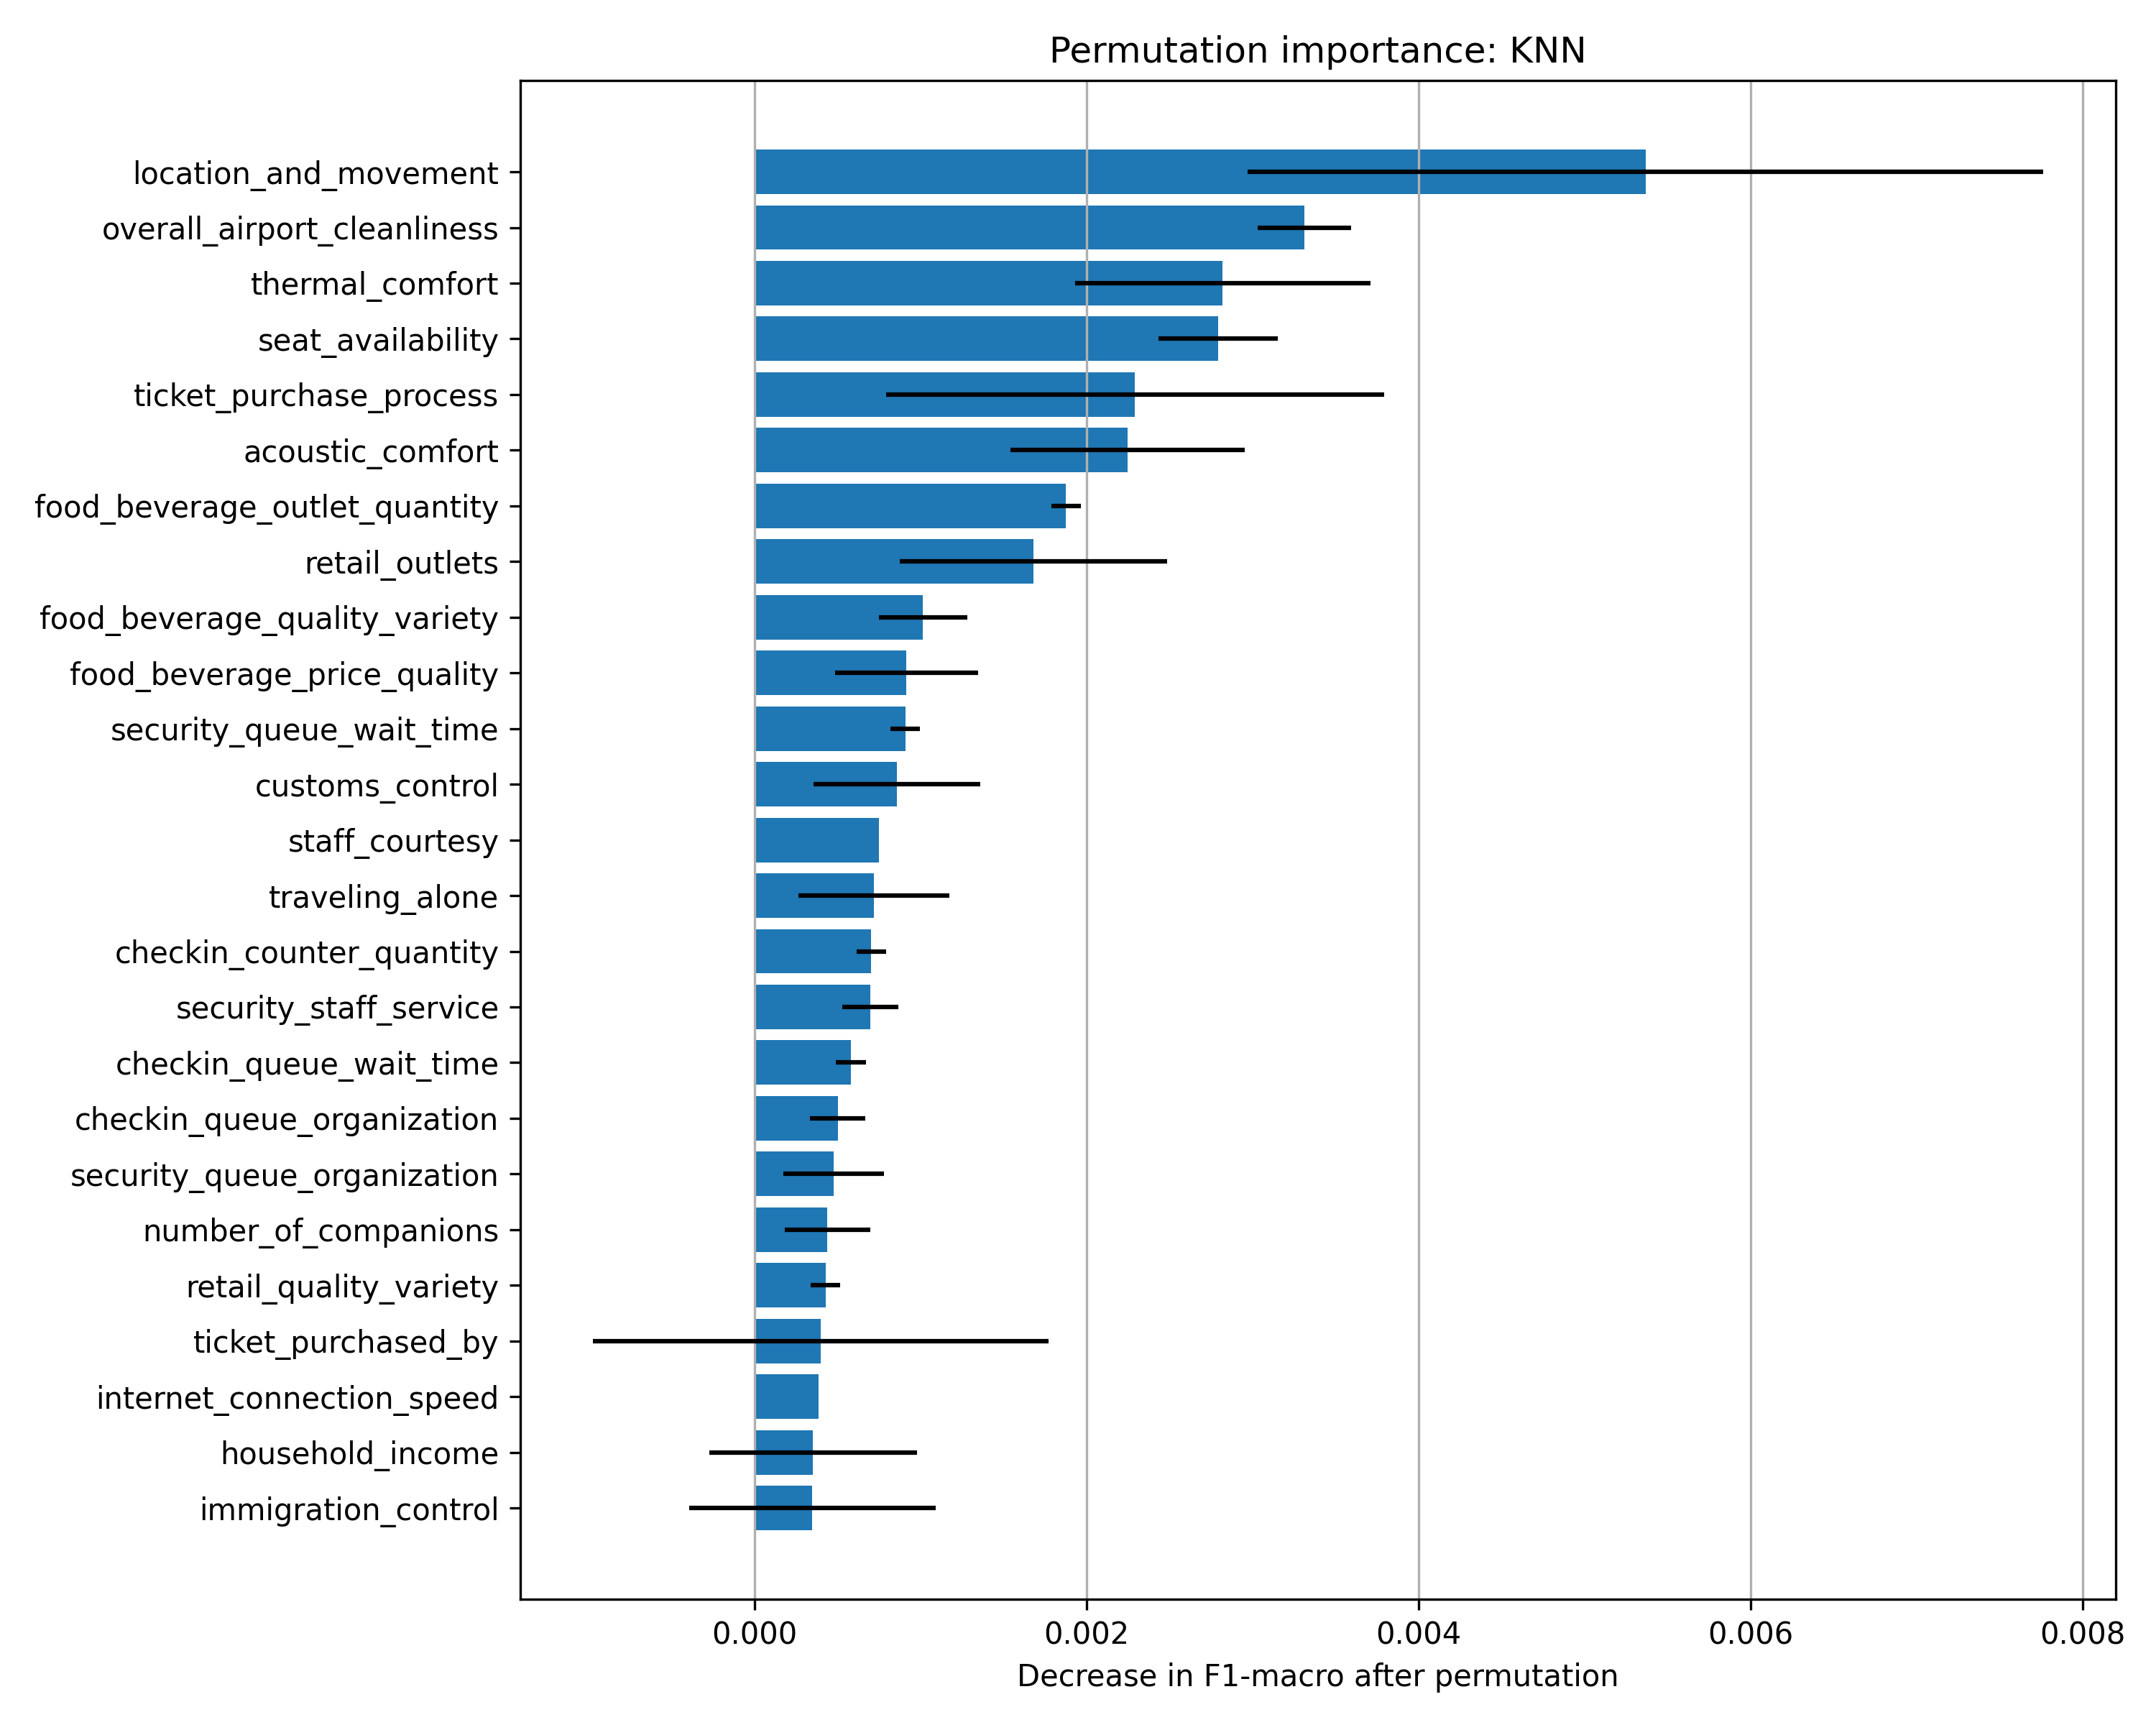
\includegraphics[width=0.82\textwidth]{knn_images/knn_permutation_importance.png}
\caption{Permutation importance: KNN}
\end{figure}
\begin{figure}[H]
\centering
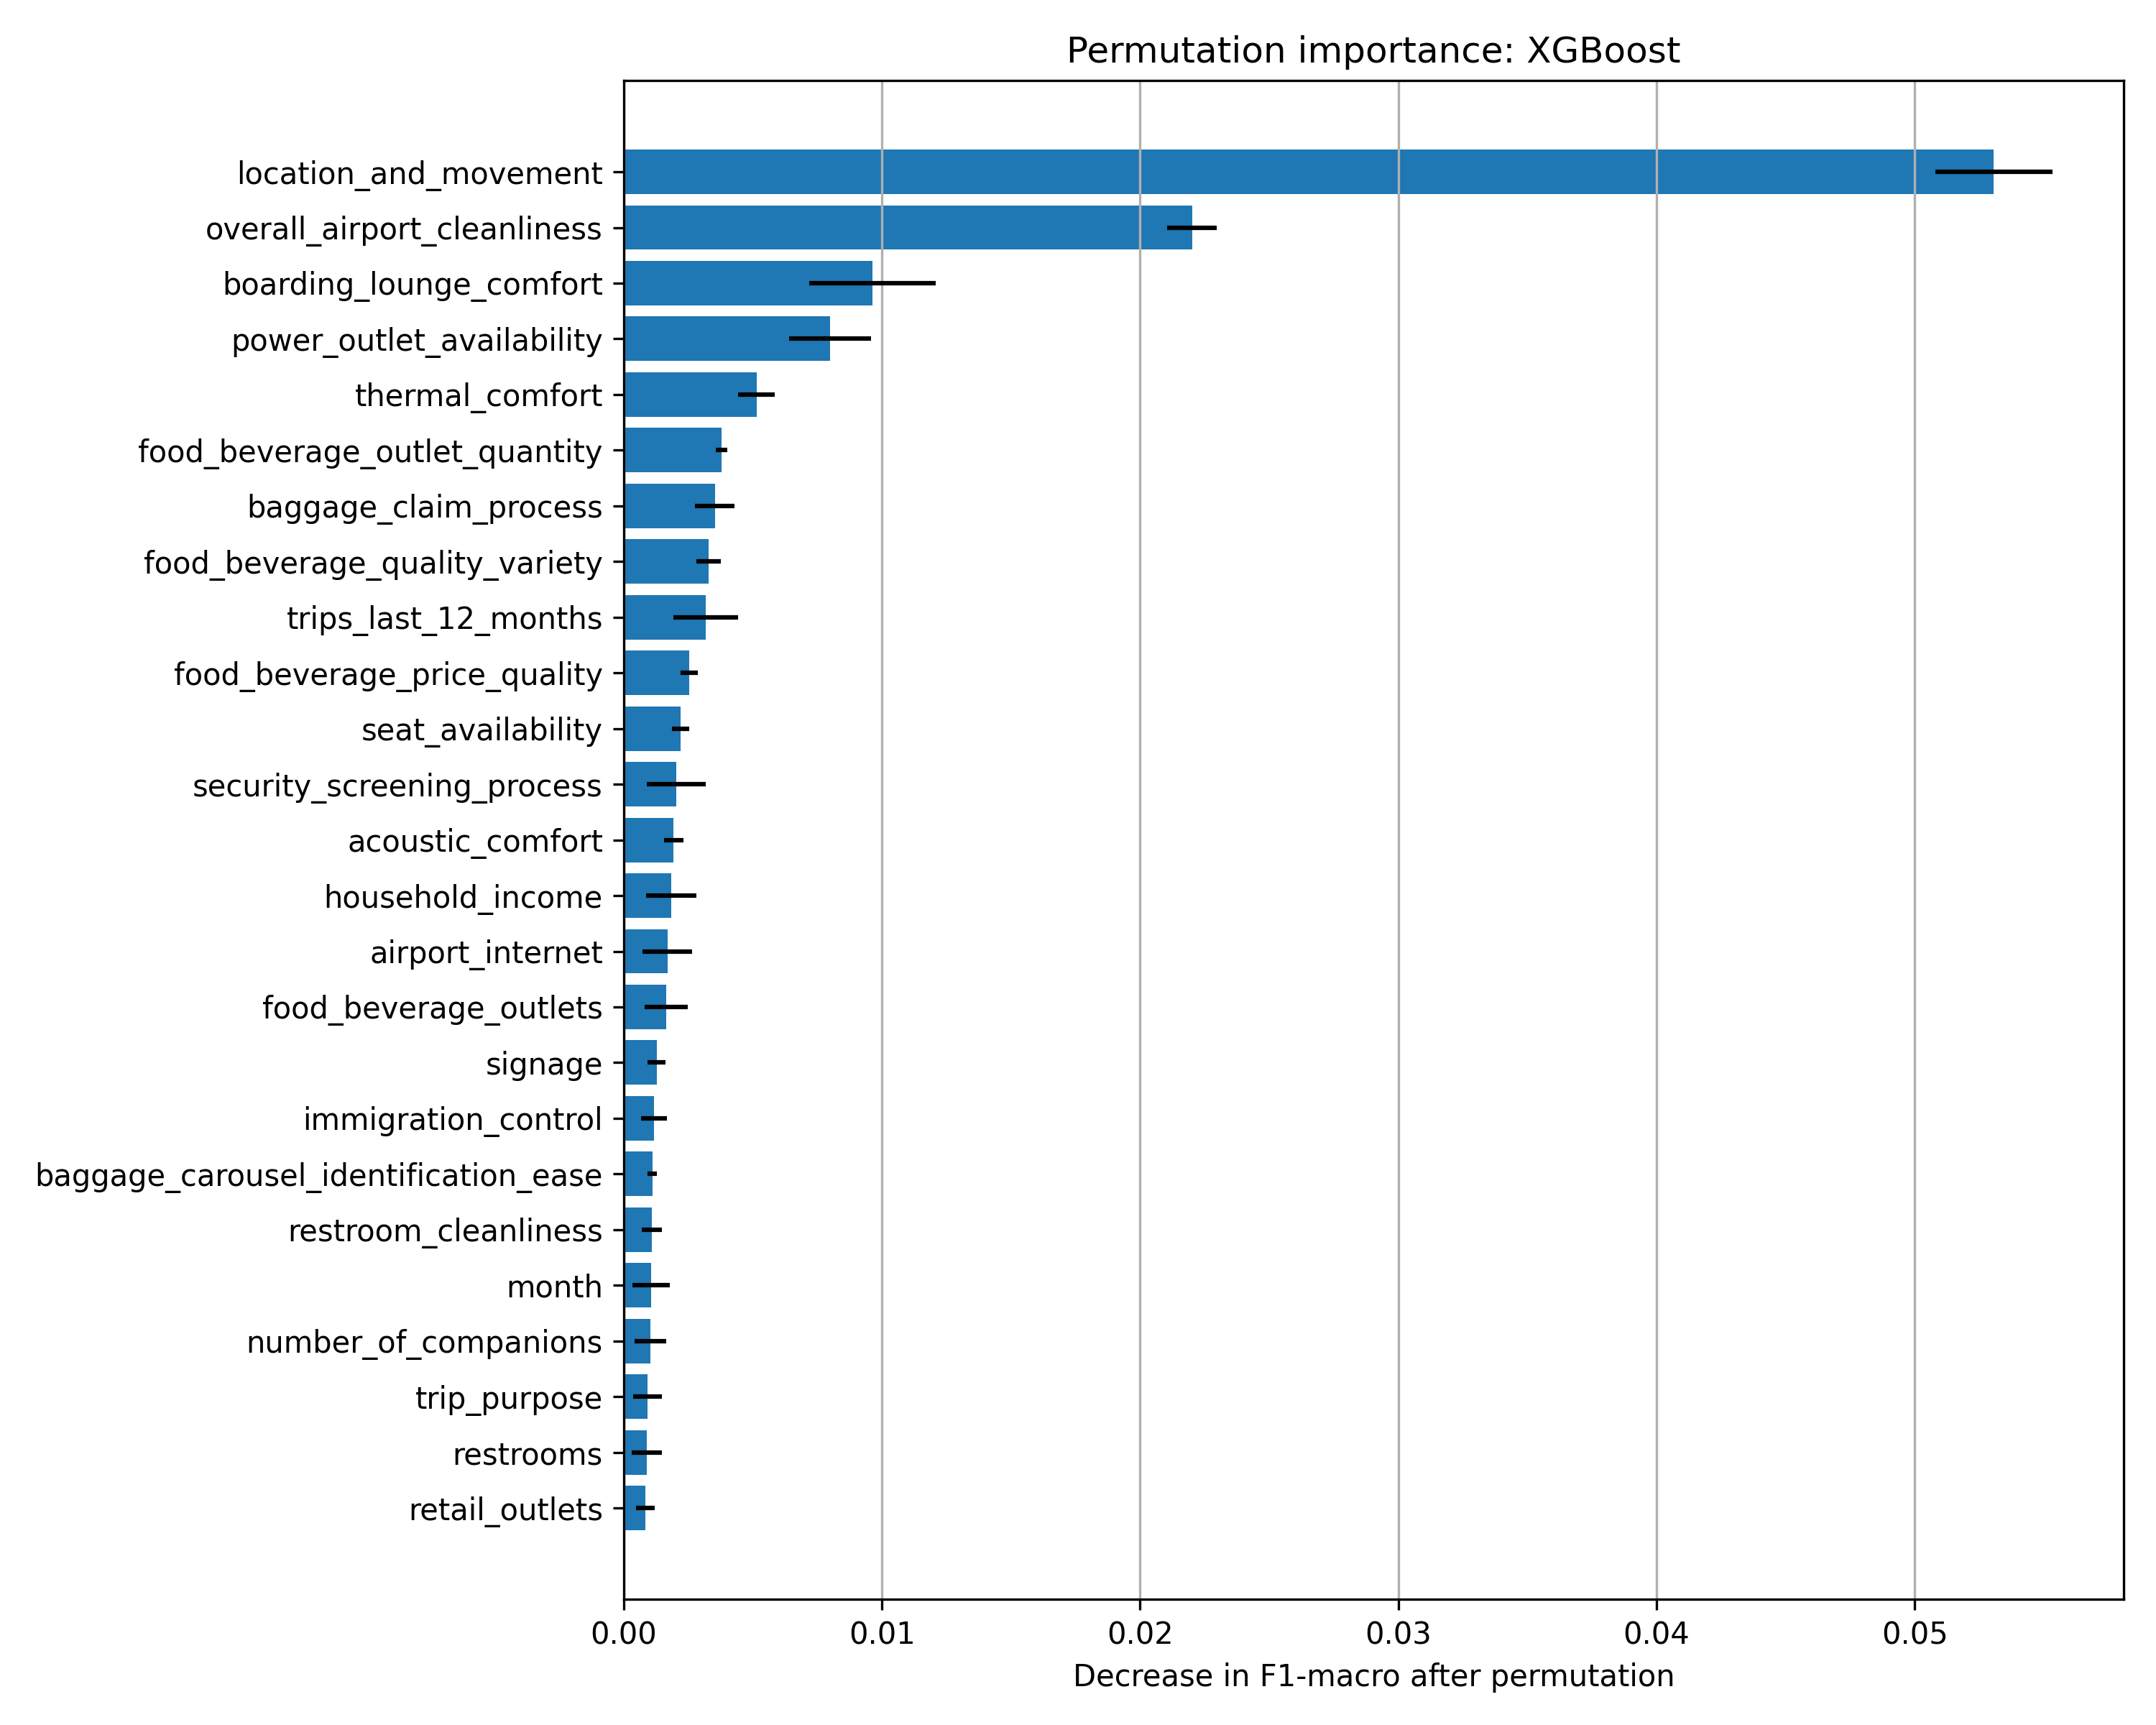
\includegraphics[width=0.82\textwidth]{xgboost_images/xgboost_permutation_importance.png}
\caption{Permutation importance: XGBoost}
\end{figure}
\begin{figure}[H]
\centering
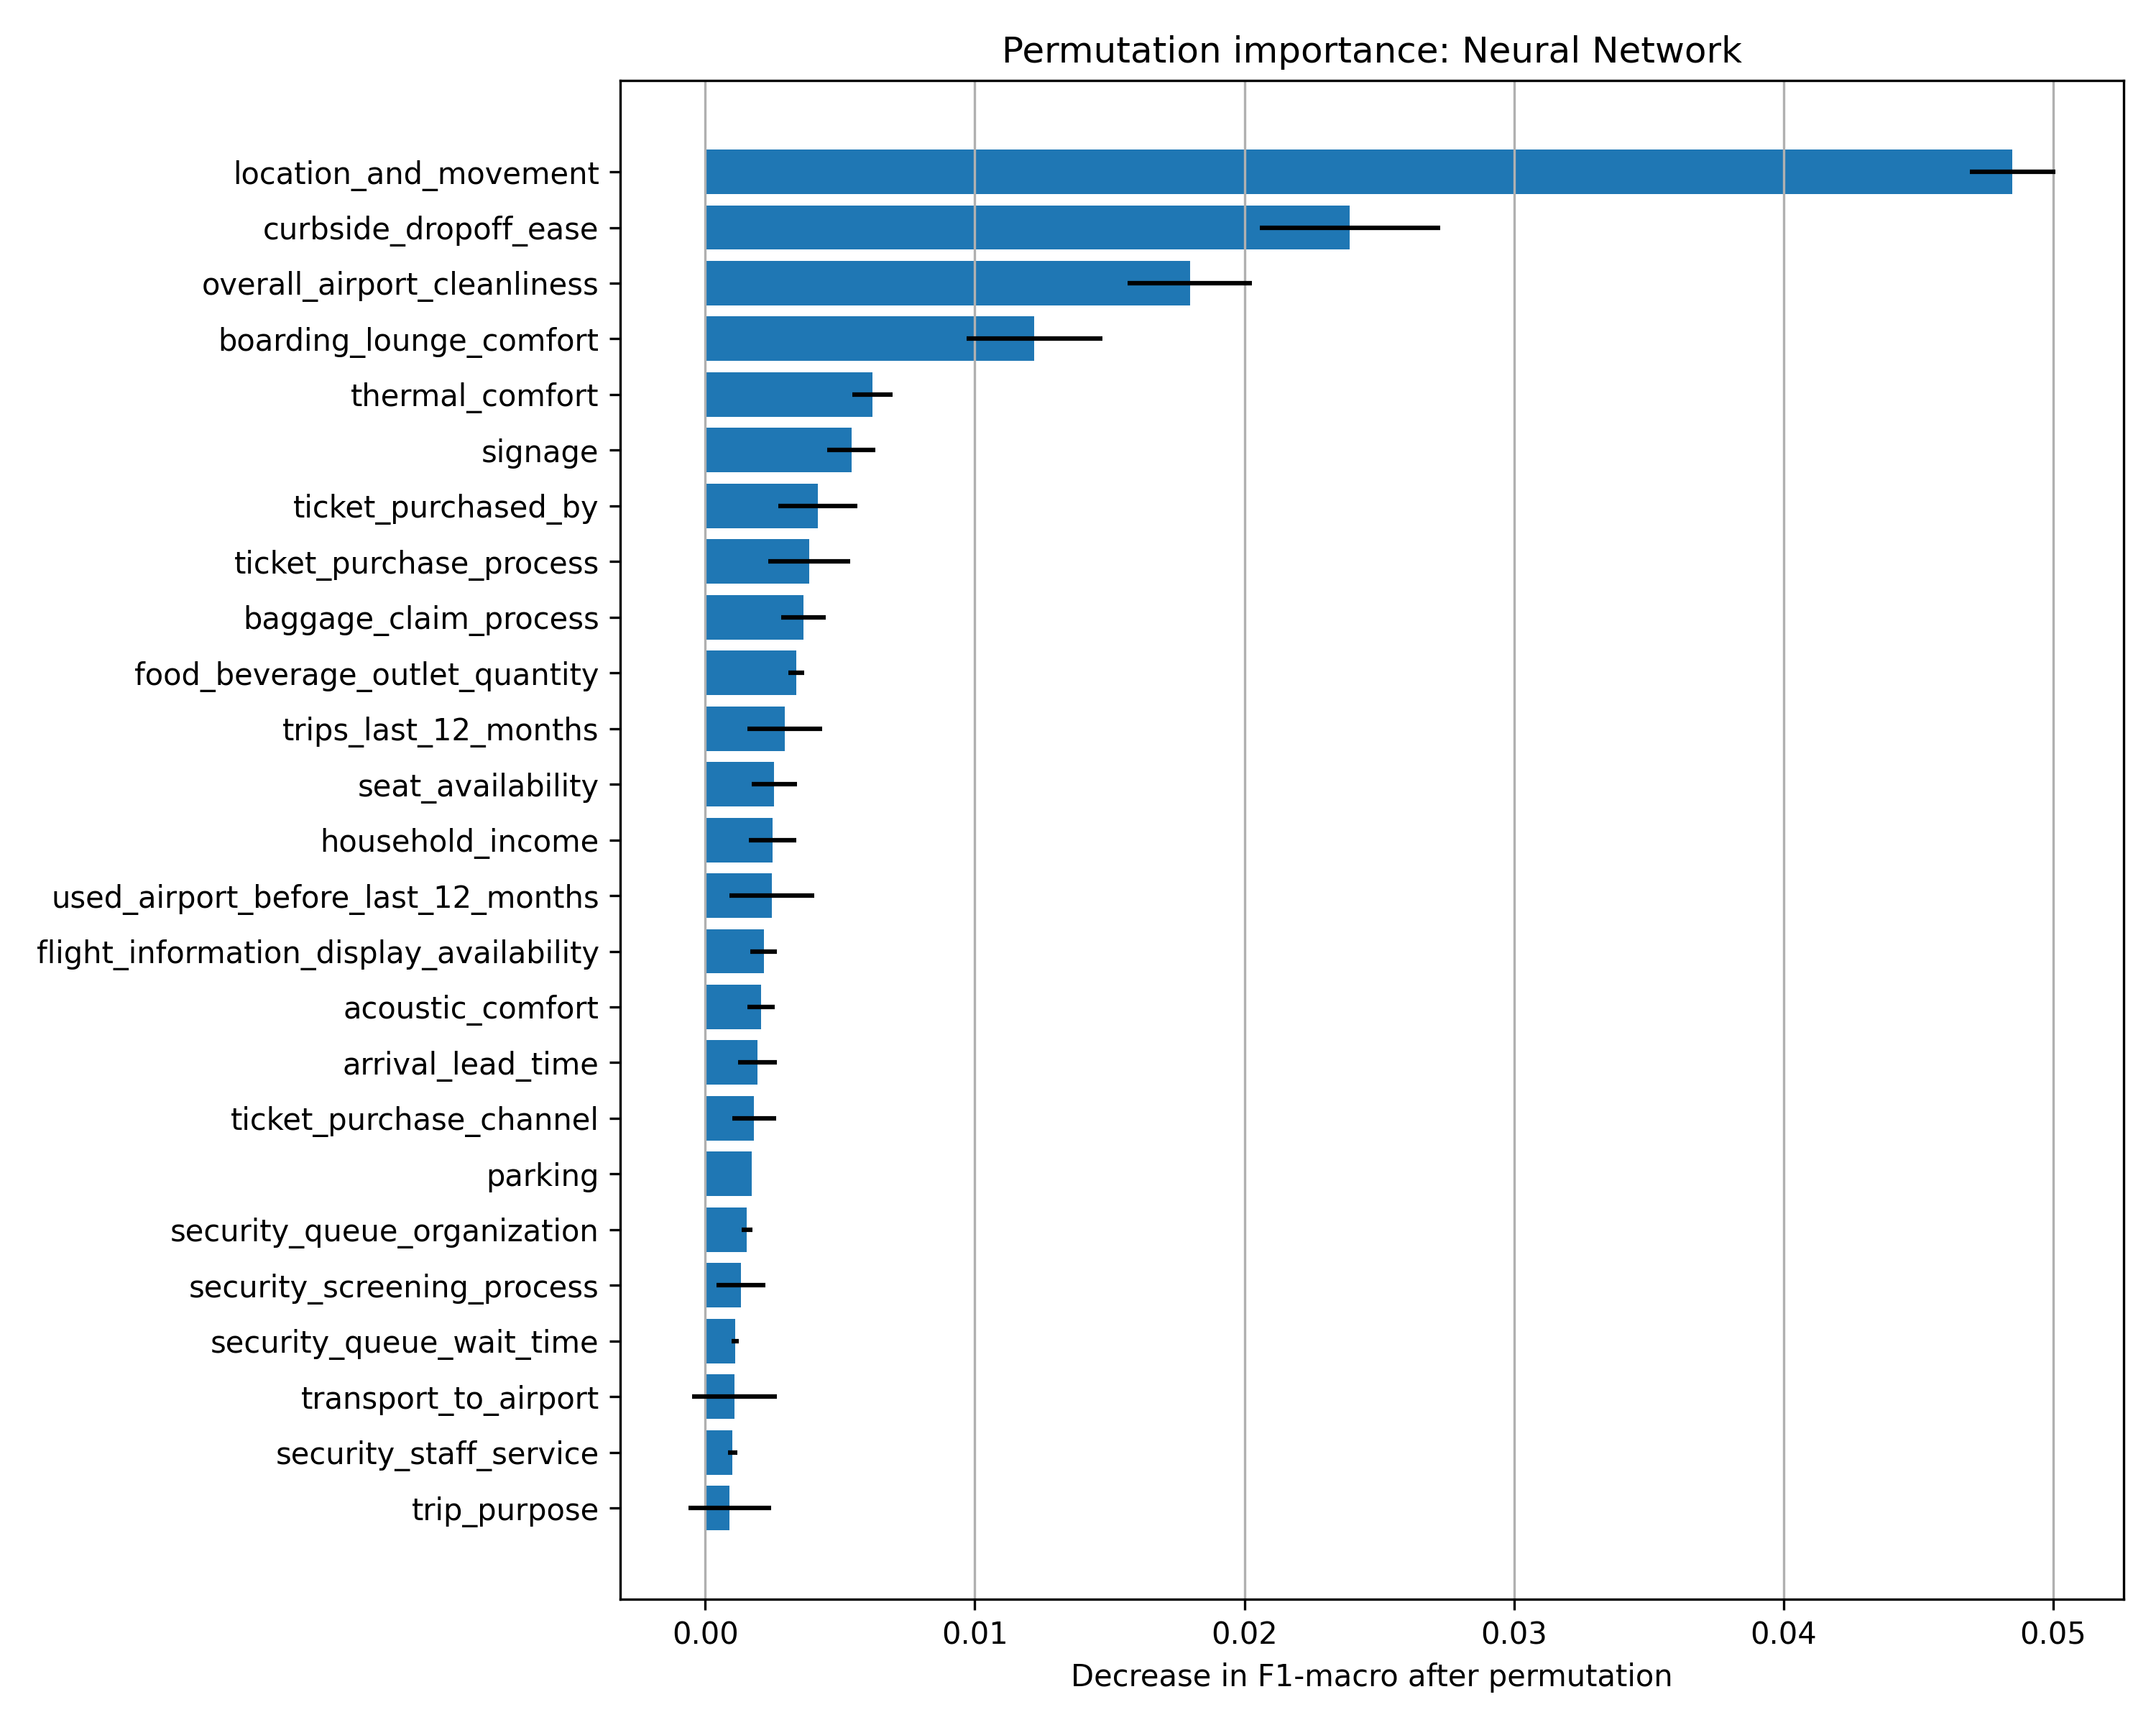
\includegraphics[width=0.82\textwidth]{neural_network_images/neural_network_permutation_importance.png}
\caption{Permutation importance: Neural Network}
\end{figure}

Во всех сильных моделях среди наиболее важных признаков встречаются оценки перемещения и навигации в аэропорту, чистоты аэропорта, удобства высадки и другие элементы пассажирского процесса. Наиболее стабильным признаком оказался \texttt{location\_and\_movement}: он занимает первое место во всех моделях. Это показывает, что итоговая удовлетворенность существенно связана не только с характеристиками рейса, но и с качеством аэропортовой инфраструктуры и отдельных процедур обслуживания. Практически такой результат означает, что улучшение навигации, чистоты, комфорта зоны ожидания и смежных сервисных процессов может быть более эффективным направлением работы, чем оптимизация только отдельных параметров перелета.


\chapter{Применение моделей машинного обучения на практике}
Результаты работы могут быть использованы в системе поддержки принятия решений авиакомпании или аэропорта. Модель прогнозирования удовлетворенности позволяет заранее выделять пассажиров с высоким риском неудовлетворенности и анализировать факторы, которые наиболее сильно влияют на итоговую оценку клиента.

Один из прикладных сценариев состоит в приоритизации улучшений сервиса. Если модель показывает, что определенные признаки, например навигация в аэропорту, чистота, время ожидания или качество процесса получения багажа, существенно влияют на вероятность удовлетворенности, то организация может направлять ресурсы именно на эти элементы обслуживания. Такой подход отличается от простого описательного анализа тем, что учитывает совместное влияние признаков и позволяет оценивать потенциальный эффект изменений.

\begin{figure}[H]
\centering
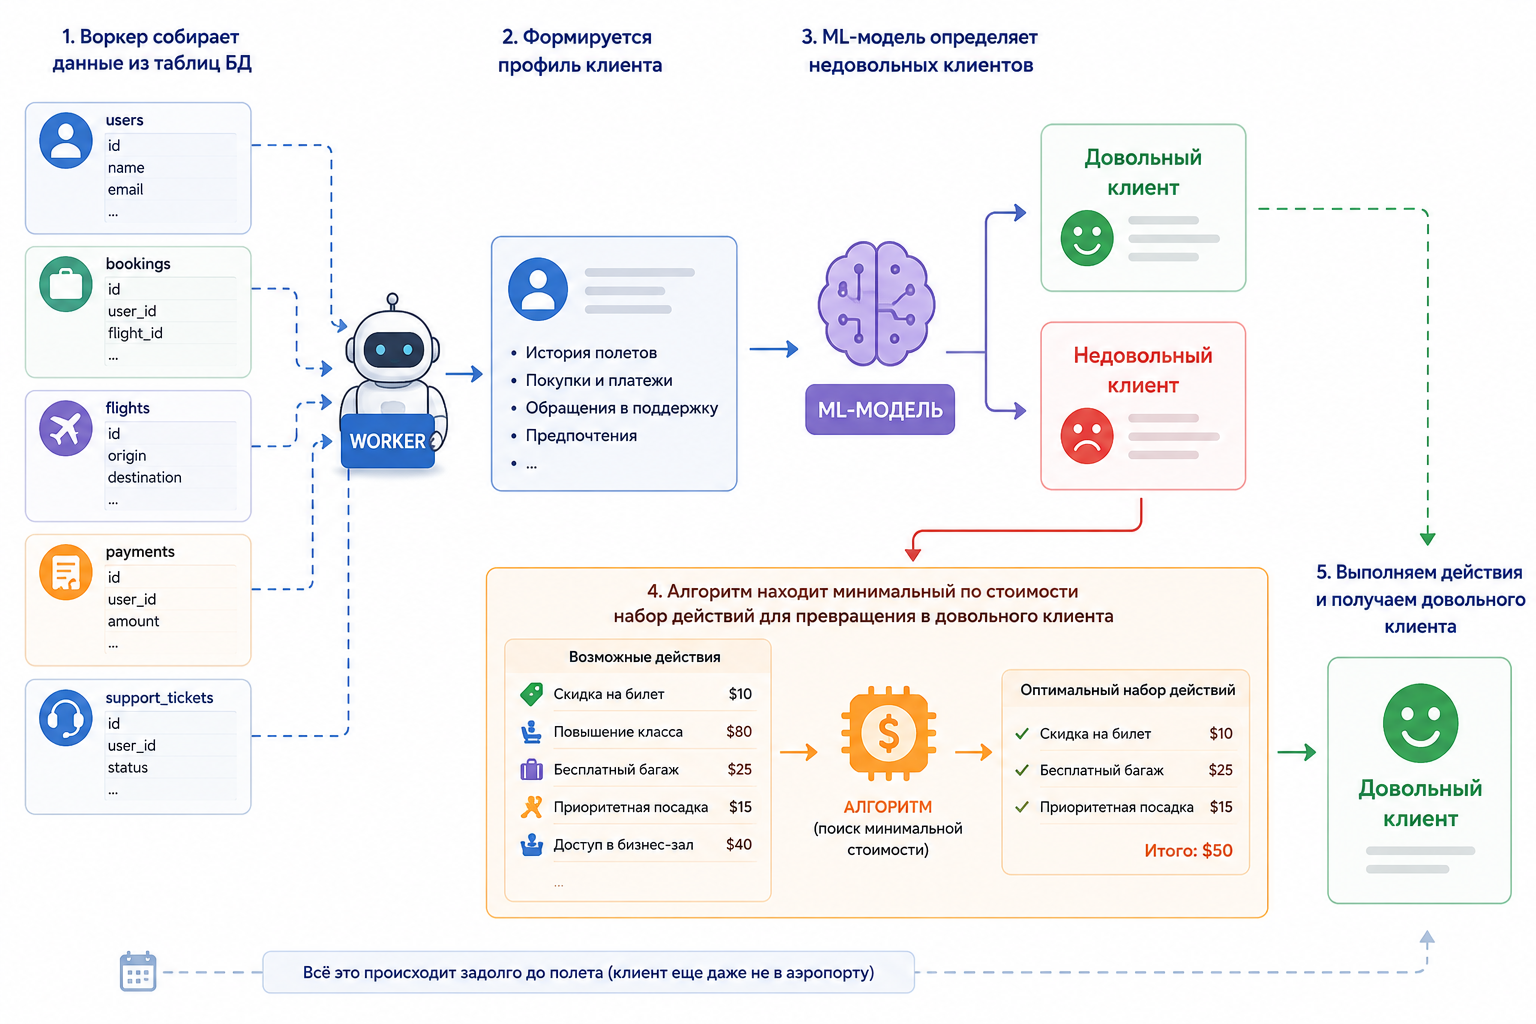
\includegraphics[width=0.95\textwidth]{research_docx_images/word/media/image3.png}
\caption{Сценарий раннего выявления недовольных клиентов на основе данных авиакомпании}
\end{figure}

В работе также реализована функция поиска минимально затратного набора изменений признаков, переводящего клиента в класс удовлетворенных пассажиров с точки зрения обученной модели. Формально эта задача рассматривается как поиск пути в графе состояний: вершинами являются возможные состояния клиента, а ребрами --- допустимые изменения отдельных признаков с заданной стоимостью. Алгоритм находит состояние, в котором модель прогнозирует положительный класс, с минимальной суммарной стоимостью переходов. Такой инструмент может использоваться как прототип рекомендательной логики для выбора наиболее эффективных управленческих действий.

\begin{figure}[H]
\centering
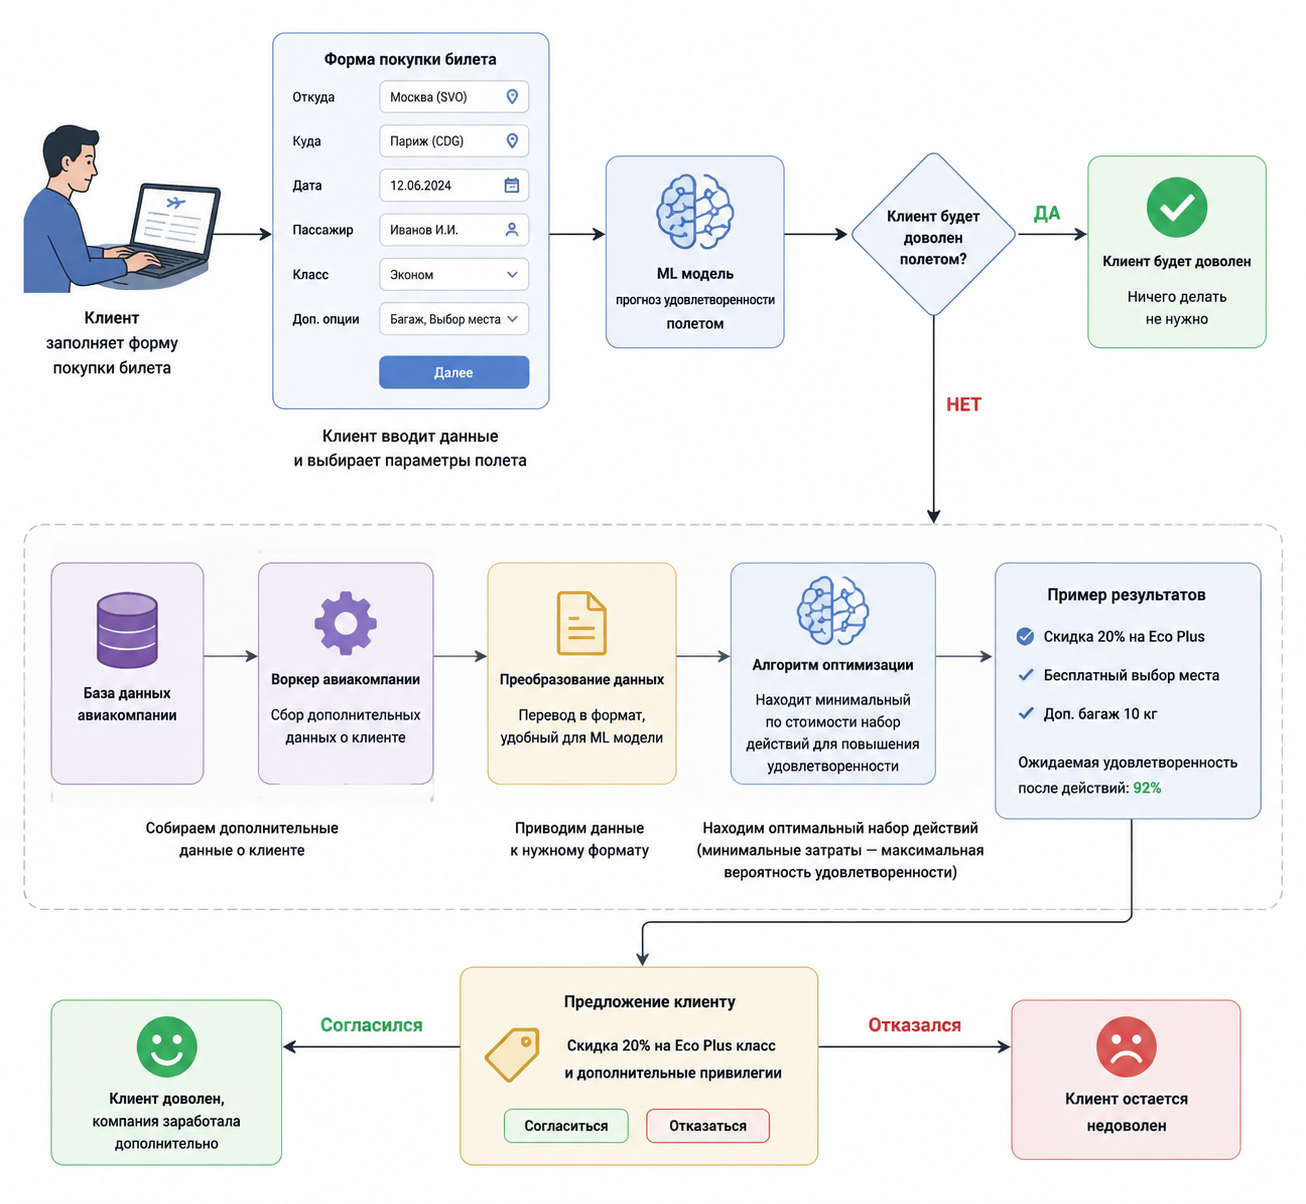
\includegraphics[width=0.95\textwidth]{research_docx_images/word/media/image1.png}
\caption{Пример использования модели и алгоритма оптимизации на этапе покупки билета}
\end{figure}

Важно подчеркнуть, что подобная функция не должна использоваться как автоматическая система принятия решений без экспертной проверки. Ее результаты зависят от качества модели, корректности заданных стоимостей изменений и полноты данных. Тем не менее она демонстрирует, как классификационная модель может быть связана с практической задачей оптимизации клиентского опыта.

Еще один практический сценарий связан с тестированием новых сервисных стратегий. В традиционном A/B-тестировании часть клиентов сталкивается с новой стратегией напрямую, и при неудачном решении компания может получить рост недовольства, снижение лояльности и финансовые потери. ML-модель позволяет предварительно смоделировать реакцию клиентов на исторических данных, оценить риск запуска стратегии и отобрать только те варианты, которые имеют высокую вероятность положительного эффекта.

\begin{figure}[H]
\centering
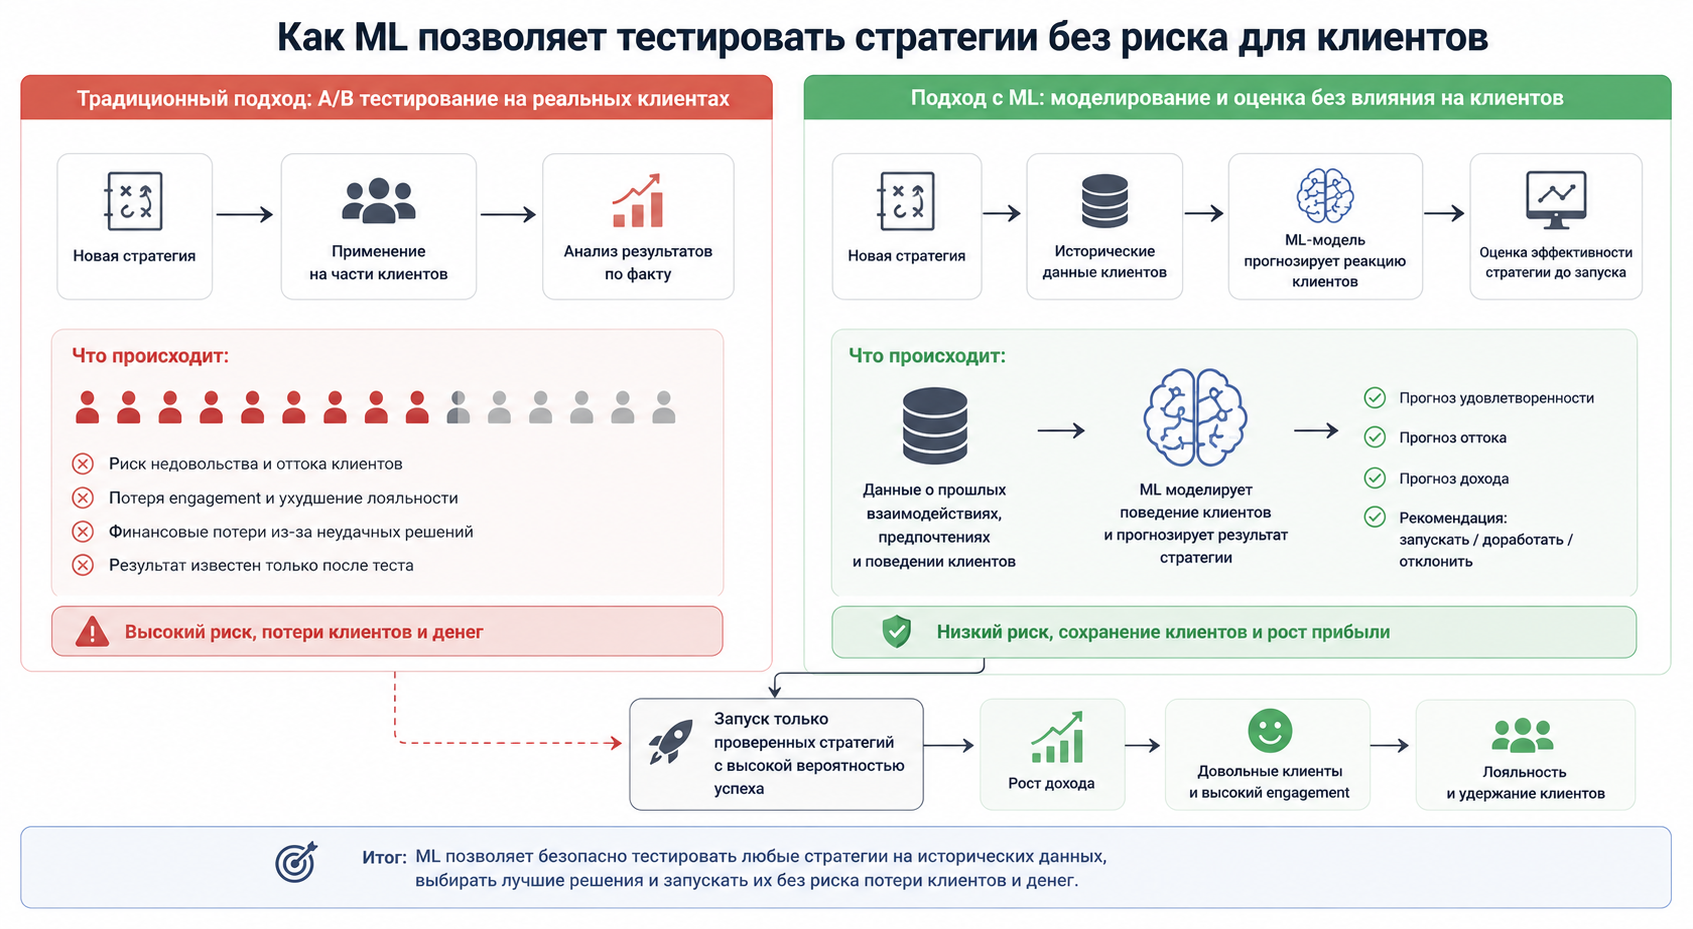
\includegraphics[width=0.95\textwidth]{research_docx_images/word/media/image2.png}
\caption{Использование ML-модели для безопасного предварительного тестирования сервисных стратегий}
\end{figure}

\chapter*{Заключение}
\addcontentsline{toc}{chapter}{Заключение}
В ходе работы была решена задача сравнительного исследования моделей машинного обучения для прогнозирования удовлетворенности пассажиров авиаперевозок. Был проведен анализ первичного Kaggle-датасета, по результатам которого было принято решение отказаться от него из-за подозрительно высоких метрик и недостаточной проверяемости источника. В качестве основного источника были использованы данные пассажирских опросов Министерства транспорта Бразилии.

Был разработан процесс формирования итогового сбалансированного датасета, включающий объединение файлов опросов, нормализацию структуры, обработку методологических пропусков, создание индикаторов применимости вопросов и балансировку классов. Итоговый датасет содержит 57514 наблюдений и используется для бинарной классификации удовлетворенности пассажиров.

Были обучены и сравнены шесть моделей: Logistic Regression, KNN, Decision Tree, Random Forest, XGBoost и Neural Network. Для всех моделей применялась единая схема preprocessing и кросс-валидации. Лучшие результаты показал XGBoost, что подтверждает эффективность градиентного бустинга для табличных данных со смешанными признаками. Нейронная сеть также показала конкурентоспособное качество, но не превзошла XGBoost. Более простые модели оказались полезны как базовые и интерпретируемые ориентиры.

Дополнительно были проведены анализ порога классификации, анализ ошибок, fairness analysis, robustness check, построение кривых обучения и оценка permutation importance. Это позволило оценить модели не только по среднему качеству классификации, но и по устойчивости, интерпретируемости и применимости в практическом сценарии. Полученные результаты могут быть использованы как основа для системы поддержки принятия решений, направленной на улучшение пассажирского опыта.

\begin{thebibliography}{99}
\bibitem{hastie} Hastie T., Tibshirani R., Friedman J. The Elements of Statistical Learning. Springer, 2009. URL: \url{https://hastie.su.domains/ElemStatLearn/download.html} (дата обращения: 16.05.2026).
\bibitem{bishop} Bishop C.M. Pattern Recognition and Machine Learning. Springer, 2006.
\bibitem{breiman-rf} Breiman L. Random Forests // Machine Learning. 2001. Vol. 45. P. 5--32.
\bibitem{cart} Breiman L., Friedman J.H., Olshen R.A., Stone C.J. Classification and Regression Trees. Wadsworth, 1984.
\bibitem{knn} Cover T., Hart P. Nearest Neighbor Pattern Classification // IEEE Transactions on Information Theory. 1967. Vol. 13, No. 1. P. 21--27.
\bibitem{xgboost} Chen T., Guestrin C. XGBoost: A Scalable Tree Boosting System // Proceedings of the 22nd ACM SIGKDD International Conference on Knowledge Discovery and Data Mining. 2016. P. 785--794. URL: \url{https://arxiv.org/abs/1603.02754} (дата обращения: 16.05.2026).
\bibitem{sklearn} Scikit-learn developers. Scikit-learn User Guide. URL: \url{https://scikit-learn.org/stable/user_guide.html} (дата обращения: 16.05.2026).
\bibitem{kaggle-old} Teejmahal20. Airline Passenger Satisfaction Dataset. URL: \url{https://www.kaggle.com/datasets/teejmahal20/airline-passenger-satisfaction} (дата обращения: 16.05.2026).
\bibitem{john-customer-satisfaction} John D. Passenger Satisfaction / Customer Satisfaction Dataset. URL: \url{https://www.kaggle.com/datasets/johndddddd/customer-satisfaction} (дата обращения: 16.05.2026).
\bibitem{kaggle-source-discussion} Kaggle. Discussion for Passenger Satisfaction Dataset: data source question. URL: \url{https://www.kaggle.com/datasets/johndddddd/customer-satisfaction/discussion/67167} (дата обращения: 16.05.2026).
\bibitem{coursera-google-da} Coursera. Google Data Analytics Professional Certificate. URL: \url{https://www.coursera.org/professional-certificates/google-data-analytics} (дата обращения: 16.05.2026).
\bibitem{iit-roorkee-project} Mittal N., Sagar A. Capstone Project: Airline Passenger Satisfaction. PG Certification in AI-ML and Data Science by IIT Roorkee. URL: \url{https://pt.scribd.com/presentation/738158403/Capstone-Project-Airline-Passenger-Satisfaction} (дата обращения: 16.05.2026).
\bibitem{brazil-data} Ministério dos Transportes do Brasil. Pesquisa de satisfação do passageiro em aeroportos. URL: \url{https://dados.transportes.gov.br/dataset/pesquisa-de-satisfacao-do-passageiro-em-aeroportos} (дата обращения: 16.05.2026).
\bibitem{icao-ai} ICAO. Global aviation leaders chart path for artificial intelligence integration. URL: \url{https://www.icao.int/news/global-aviation-leaders-chart-path-artificial-intelligence-integration-antalya-conference} (дата обращения: 16.05.2026).
\bibitem{iata-data} IATA. Recognizing the future importance of data. URL: \url{https://airlines.iata.org/2025/05/15/recognizing-future-importance-data} (дата обращения: 16.05.2026).
\bibitem{aci-digital} ACI World. The Acceleration of Digital Transformation in Airports. URL: \url{https://blog.aci.aero/the-acceleration-of-digital-transformation-in-airports/} (дата обращения: 16.05.2026).
\bibitem{aci-asq} ACI World. Airport Service Quality (ASQ). URL: \url{https://aci.aero/programs-and-services/asq/} (дата обращения: 16.05.2026).
\bibitem{easa-roadmap} EASA. Artificial Intelligence Roadmap 2.0. URL: \url{https://www.easa.europa.eu/it/document-library/general-publications/easa-artificial-intelligence-roadmap-20} (дата обращения: 16.05.2026).
\bibitem{easa-concept} EASA. Artificial Intelligence Concept Paper Issue 2. URL: \url{https://www.easa.europa.eu/nl/newsroom-and-events/news/easa-publishes-artificial-intelligence-concept-paper-issue-2-guidance} (дата обращения: 16.05.2026).
\bibitem{nist-rmf} NIST. AI Risk Management Framework. URL: \url{https://www.nist.gov/itl/ai-risk-management-framework} (дата обращения: 16.05.2026).
\bibitem{nist-characteristics} NIST. AI RMF: Characteristics of Trustworthy AI. URL: \url{https://airc.nist.gov/airmf-resources/airmf/3-sec-characteristics/} (дата обращения: 16.05.2026).
\end{thebibliography}

\appendix
\chapter{Электронные ресурсы проекта}
Полный исходный код, использованный для подготовки данных, обучения моделей, расчета метрик и построения визуализаций, размещен в GitHub-репозитории:\\
\url{https://github.com/rustam432184798213651/machine_learning_models_study}

Использованный итоговый датасет опубликован на Kaggle:\\
\url{https://www.kaggle.com/datasets/rustam32/real-airline-passenger-satisfaction-dataset/data}

\end{document}
